% Run LaTeX on this file several times to get Table of Contents,
%% cross-references, and citations.

\documentclass[11pt]{book}
\usepackage{gvv-book}
\usepackage{gvv}
\usepackage{vaman/uart/figs/circuit}        
%\usepackage{Wiley-AuthoringTemplate}
\usepackage[sectionbib,authoryear]{natbib}% for name-date citation comment the below line
%\usepackage[sectionbib,numbers]{natbib}% for numbered citation comment the above line

%%********************************************************************%%
%%       How many levels of section head would you like numbered?     %%
%% 0= no section numbers, 1= section, 2= subsection, 3= subsubsection %%
\setcounter{secnumdepth}{3}
%%********************************************************************%%
%%**********************************************************************%%
%%     How many levels of section head would you like to appear in the  %%
%%				Table of Contents?			%%
%% 0= chapter, 1= section, 2= subsection, 3= subsubsection titles.	%%
\setcounter{tocdepth}{2}
%%**********************************************************************%%

%\includeonly{ch01}
\makeindex

\begin{document}

\frontmatter
%%%%%%%%%%%%%%%%%%%%%%%%%%%%%%%%%%%%%%%%%%%%%%%%%%%%%%%%%%%%%%%%
%% Title Pages
%% Wiley will provide title and copyright page, but you can make
%% your own titlepages if you'd like anyway
%% Setting up title pages, type in the appropriate names here:

\booktitle{Digital Design}

\subtitle{Through Embedded Programming}

\AuAff{G. V. V. Sharma}


%% \\ will start a new line.
%% You may add \affil{} for affiliation, ie,
%\authors{Robert M. Groves\\
%\affil{Universitat de les Illes Balears}
%Floyd J. Fowler, Jr.\\
%\affil{University of New Mexico}
%}

%% Print Half Title and Title Page:
%\halftitlepage
\titlepage

%%%%%%%%%%%%%%%%%%%%%%%%%%%%%%%%%%%%%%%%%%%%%%%%%%%%%%%%%%%%%%%%
%% Copyright Page

\begin{copyrightpage}{2022}
%Title, etc
\end{copyrightpage}

% Note, you must use \ to start indented lines, ie,
% 
% \begin{copyrightpage}{2004}
% Survey Methodology / Robert M. Groves . . . [et al.].
% \       p. cm.---(Wiley series in survey methodology)
% \    ``Wiley-Interscience."
% \    Includes bibliographical references and index.
% \    ISBN 0-471-48348-6 (pbk.)
% \    1. Surveys---Methodology.  2. Social 
% \  sciences---Research---Statistical methods.  I. Groves, Robert M.  II. %
% Series.\\

% HA31.2.S873 2004
% 001.4'33---dc22                                             2004044064
% \end{copyrightpage}

%%%%%%%%%%%%%%%%%%%%%%%%%%%%%%%%%%%%%%%%%%%%%%%%%%%%%%%%%%%%%%%%
%% Only Dedication (optional) 

%\dedication{To my parents}

\tableofcontents

%\listoffigures %optional
%\listoftables  %optional

%% or Contributor Page for edited books
%% before \tableofcontents

%%%%%%%%%%%%%%%%%%%%%%%%%%%%%%%%%%%%%%%%%%%%%%%%%%%%%%%%%%%%%%%%
%  Contributors Page for Edited Book
%%%%%%%%%%%%%%%%%%%%%%%%%%%%%%%%%%%%%%%%%%%%%%%%%%%%%%%%%%%%%%%%

% If your book has chapters written by different authors,
% you'll need a Contributors page.

% Use \begin{contributors}...\end{contributors} and
% then enter each author with the \name{} command, followed
% by the affiliation information.

% \begin{contributors}
% \name{Masayki Abe,} Fujitsu Laboratories Ltd., Fujitsu Limited, Atsugi, Japan
%
% \name{L. A. Akers,} Center for Solid State Electronics Research, Arizona State University, Tempe, Arizona
%
% \name{G. H. Bernstein,} Department of Electrical and Computer Engineering, University of Notre Dame, Notre Dame, South Bend, Indiana; formerly of
% Center for Solid State Electronics Research, Arizona
% State University, Tempe, Arizona 
% \end{contributors}

%%%%%%%%%%%%%%%%%%%%%%%%%%%%%%%%%%%%%%%%%%%%%%%%%%%%%%%%%%%%%%%%
% Optional Foreword:

%\begin{foreword}
%\lipsum[1-2]
%\end{foreword}

%%%%%%%%%%%%%%%%%%%%%%%%%%%%%%%%%%%%%%%%%%%%%%%%%%%%%%%%%%%%%%%%
% Optional Preface:

%\begin{preface}
%\lipsum[1-1]
%\prefaceauthor{}
%\where{place\\
% date}
%\end{preface}

% ie,
% \begin{preface}
% This is an example preface.
% \prefaceauthor{R. K. Watts}
% \where{Durham, North Carolina\\
% September, 2004}

%%%%%%%%%%%%%%%%%%%%%%%%%%%%%%%%%%%%%%%%%%%%%%%%%%%%%%%%%%%%%%%%
% Optional Acknowledgments:

%\acknowledgments
%\lipsum[1-2]
%\authorinitials{I. R. S.}  

%%%%%%%%%%%%%%%%%%%%%%%%%%%%%%%%
%% Glossary Type of Environment:

% \begin{glossary}
% \term{<term>}{<description>}
% \end{glossary}

%%%%%%%%%%%%%%%%%%%%%%%%%%%%%%%%
%\begin{acronyms}
%\acro{ASTA}{Arrivals See Time Averages}
%\acro{BHCA}{Busy Hour Call Attempts}
%\acro{BR}{Bandwidth Reservation}
%\acro{b.u.}{bandwidth unit(s)}
%\acro{CAC}{Call / Connection Admission Control}
%\acro{CBP}{Call Blocking Probability(-ies)}
%\acro{CCS}{Centum Call Seconds}
%\acro{CDTM}{Connection Dependent Threshold Model}
%\acro{CS}{Complete Sharing}
%\acro{DiffServ}{Differentiated Services}
%\acro{EMLM}{Erlang Multirate Loss Model}
%\acro{erl}{The Erlang unit of traffic-load}
%\acro{FIFO}{First in - First out}
%\acro{GB}{Global balance}
%\acro{GoS}{Grade of Service}
%\acro{ICT}{Information and Communication Technology}
%\acro{IntServ}{Integrated Services}
%\acro{IP}{Internet Protocol}
%\acro{ITU-T}{International Telecommunication Unit -- Standardization sector}
%\acro{LB}{Local balance}
%\acro{LHS}{Left hand side}
%\acro{LIFO}{Last in - First out}
%\acro{MMPP}{Markov Modulated Poisson Process}
%\acro{MPLS}{Multiple Protocol Labeling Switching}
%\acro{MRM}{Multi-Retry Model}
%\acro{MTM}{Multi-Threshold Model}
%\acro{PASTA}{Poisson Arrivals See Time Averages}
%\acro{PDF}{Probability Distribution Function}
%\acro{pdf}{probability density function}
%\acro{PFS}{Product Form Solution}
%\acro{QoS}{Quality of Service}
%\acro{r.v.}{random variable(s)}
%\acro{RED}{random early detection}
%\acro{RHS}{Right hand side}
%\acro{RLA}{Reduced Load Approximation}
%\acro{SIRO}{service in random order}
%\acro{SRM}{Single-Retry Model}
%\acro{STM}{Single-Threshold Model}
%\acro{TCP}{Transport Control Protocol}
%\acro{TH}{Threshold(s)}
%\acro{UDP}{User Datagram Protocol}
%\end{acronyms}

\setcounter{page}{1}

\begin{introduction}
This book introduces digital design through using the arduino framework.
\end{introduction}

\mainmatter
\chapter{Installation}
\iffalse
\let\negmedspace\undefined
\let\negthickspace\undefined
\documentclass[journal,2pt,twocolumn]{IEEEtran}
%
\usepackage{setspace}
\usepackage{gensymb}
\usepackage{xcolor}
\usepackage{caption}
%\usepackage{subcaption}
%\doublespacing
\singlespacing

%\usepackage{graphicx}
%\usepackage{amssymb}
%\usepackage{relsize}
\usepackage[cmex0]{amsmath}
\usepackage{mathtools}
%\usepackage{amsthm}
%\interdisplaylinepenalty=2500
%\savesymbol{iint}
%\usepackage{txfonts}
%\restoresymbol{TXF}{iint}
%\usepackage{wasysym}
\usepackage{amsthm}
\usepackage{mathrsfs}
\usepackage{txfonts}
\usepackage{stfloats}
\usepackage{cite}
\usepackage{cases}
\usepackage{subfig}
%\usepackage{xtab}
\usepackage{longtable}
\usepackage{multirow}
%\usepackage{algorithm}
%\usepackage{algpseudocode}
\usepackage{enumerate}
\usepackage{mathtools}
%\usepackage{eenrc}
%\usepackage[framemethod=tikz]{mdframed}
	\usepackage{listings}
\usepackage{listings}
    \usepackage[latin]{inputenc}                                 %%
    \usepackage{color}                                            %%
    \usepackage{array}                                            %%
    \usepackage{longtable}                                        %%
    \usepackage{calc}                                             %%
    \usepackage{multirow}                                         %%
    \usepackage{hhline}                                           %%
    \usepackage{ifthen}                                           %%
  %optionally (for landscape tables embedded in another document): %%
    \usepackage{lscape}     
\usepackage{tikz}
\usepackage{circuitikz}
\usepackage{karnaugh-map}
\usepackage{pgf}




%\usepackage{stmaryrd}


%\usepackage{wasysym}
%\newcounter{MYtempeqncnt}
\DeclareMathOperator*{\Res}{Res}
%\renewcommand{\baselinestretch}{2}
\renewcommand\thesection{\arabic{section}}
\renewcommand\thesubsection{\thesection\arabic{subsection}}
\renewcommand\thesubsubsection{\thesubsection\arabic{subsubsection}}

\renewcommand\thesectiondis{\arabic{section}}
\renewcommand\thesubsectiondis{\thesectiondis\arabic{subsection}}
\renewcommand\thesubsubsectiondis{\thesubsectiondis\arabic{subsubsection}}

% correct bad hyphenation here
\hyphenation{op-tical net-works semi-conduc-tor}

%\lstset{
%language=C,
%frame=single, 
%breaklines=true
%}

%\lstset{
	%%basicstyle=\small\ttfamily\bfseries,
	%%numberstyle=\small\ttfamily,
	%language=Octave,
	%backgroundcolor=\color{white},
	%%frame=single,
	%%keywordstyle=\bfseries,
	%%breaklines=true,
	%%showstringspaces=false,
	%%xleftmargin=-0mm,
	%%aboveskip=-mm,
	%%belowskip=0mm
%}

%\surroundwithmdframed[width=\columnwidth]{lstlisting}
\def\inputGnumericTable{}                                 %%
\lstset{
%language=C,
frame=single, 
breaklines=true,
columns=fullflexible,
literate = {-}{-}
}
 

\begin{document}
%

\theoremstyle{definition}
\newtheorem{theorem}{Theorem}[section]
\newtheorem{problem}{Problem}
\newtheorem{proposition}{Proposition}[section]
\newtheorem{lemma}{Lemma}[section]
\newtheorem{corollary}[theorem]{Corollary}
\newtheorem{example}{Example}[section]
\newtheorem{definition}{Definition}[section]
%\newtheorem{algorithm}{Algorithm}[section]
%\newtheorem{cor}{Corollary}
\newcommand{\BEQA}{\begin{eqnarray}}
\newcommand{\EEQA}{\end{eqnarray}}
\newcommand{\define}{\stackrel{\triangle}{=}}

\bibliographystyle{IEEEtran}
%\bibliographystyle{ieeetr}

\providecommand{\nCr}[2]{\,^{#}C_{#2}} % nCr
\providecommand{\nPr}[2]{\,^{#}P_{#2}} % nPr
\providecommand{\mbf}{\mathbf}
\providecommand{\pr}{\ensuremath{\Pr\left(#\right)}}
\providecommand{\qfunc}{\ensuremath{Q\left(#\right)}}
\providecommand{\sbrak}{\ensuremath{{}\left[#\right]}}
\providecommand{\lsbrak}{\ensuremath{{}\left[#\right}}
\providecommand{\rsbrak}{\ensuremath{{}\left#\right]}}
\providecommand{\brak}{\ensuremath{\left(#\right)}}
\providecommand{\lbrak}{\ensuremath{\left(#\right}}
\providecommand{\rbrak}{\ensuremath{\left#\right)}}
\providecommand{\cbrak}{\ensuremath{\left\{#\right\}}}
\providecommand{\lcbrak}{\ensuremath{\left\{#\right}}
\providecommand{\rcbrak}{\ensuremath{\left#\right\}}}
\providecommand{\ceil}{\left \lceil # \right \rceil }
\theoremstyle{remark}
\newtheorem{rem}{Remark}
\newcommand{\sgn}{\mathop{\mathrm{sgn}}}
\providecommand{\abs}{\left\vert#\right\vert}
\providecommand{\res}{\Res\displaylimits_{#}} 
\providecommand{\norm}{\lVert#\rVert}
\providecommand{\mtx}{\mathbf{#}}
\providecommand{\mean}{E\left[ # \right]}
\providecommand{\fourier}{\overset{\mathcal{F}}{ \rightleftharpoons}}
%\providecommand{\hilbert}{\overset{\mathcal{H}}{ \rightleftharpoons}}
\providecommand{\system}{\overset{\mathcal{H}}{ \longleftrightarrow}}
	%\newcommand{\solution}[2]{\textbf{Solution:}{#}}
\newcommand{\solution}{\noindent \textbf{Solution: }}
\providecommand{\dec}[2]{\ensuremath{\overset{#}{\underset{#2}{\gtrless}}}}


%\numberwithin{equation}{subsection}
\numberwithin{equation}{problem}
%\numberwithin{problem}{subsection}
%\numberwithin{definition}{subsection}
\makeatletter
\@addtoreset{figure}{problem}
\makeatother

\let\StandardTheFigure\thefigure
%\renewcommand{\thefigure}{\theproblem\arabic{figure}}
\renewcommand{\thefigure}{\theproblem}


%\numberwithin{figure}{subsection}

%\numberwithin{equation}{subsection}
%\numberwithin{equation}{section}
%%\numberwithin{equation}{problem}
%%\numberwithin{problem}{subsection}
\numberwithin{problem}{section}
%%\numberwithin{definition}{subsection}
%\makeatletter
%\@addtoreset{figure}{problem}
%\makeatother
\makeatletter
\@addtoreset{table}{problem}
\makeatother

\let\StandardTheFigure\thefigure
\let\StandardTheTable\thetable
%%\renewcommand{\thefigure}{\theproblem\arabic{figure}}
%\renewcommand{\thefigure}{\theproblem}
\renewcommand{\thetable}{\theproblem}
%%\numberwithin{figure}{section}

%%\numberwithin{figure}{subsection}



\def\putbox##2#3{\makebox[0in][l]{\makebox[#][l]{}\raisebox{\baselineskip}[0in][0in]{\raisebox{#2}[0in][0in]{#3}}}}
     \def\rightbox#{\makebox[0in][r]{#}}
     \def\centbox#{\makebox[0in]{#}}
     \def\topbox#{\raisebox{-\baselineskip}[0in][0in]{#}}
     \def\midbox#{\raisebox{-05\baselineskip}[0in][0in]{#}}

\vspace{3cm}

\title{ 
%	\logo{
Platformio on Android-Termux
%	}
}



% paper title
% can use linebreaks \\ within to get better formatting as desired
%\title{Matrix Analysis through Octave}
%
%
% author names and IEEE memberships
% note positions of commas and nonbreaking spaces ( ~ ) LaTeX will not break
% a structure at a ~ so this keeps an author's name from being broken across
% two lines
% use \thanks{} to gain access to the first footnote area
% a separate \thanks must be used for each paragraph as LaTeX2e's \thanks
% was not built to handle multiple paragraphs
%

\author{G V V Sharma$^{*}$% <-this % stops a space
\thanks{*The author is with the Department
of Electrical Engineering, Indian Institute of Technology, Hyderabad
502285 India e-mail:  gadepall@iithacin All content in this manual is released under GNU GPL  Free and open source}% <-this % stops a space
%\thanks{J Doe and J Doe are with Anonymous University}% <-this % stops a space
%\thanks{Manuscript received April 9, 2005; revised January , 2007}}
}
% note the % following the last \IEEEmembership and also \thanks - 
% these prevent an unwanted space from occurring between the last author name
% and the end of the author line ie, if you had this:
% 
% \author{lastname \thanks{} \thanks{} }
%                     ^------------^------------^----Do not want these spaces!
%
% a space would be appended to the last name and could cause every name on that
% line to be shifted left slightly This is one of those "LaTeX things" For
% instance, "\textbf{A} \textbf{B}" will typeset as "A B" not "AB" To get
% "AB" then you have to do: "\textbf{A}\textbf{B}"
% \thanks is no different in this regard, so shield the last } of each \thanks
% that ends a line with a % and do not let a space in before the next \thanks
% Spaces after \IEEEmembership other than the last one are OK (and needed) as
% you are supposed to have spaces between the names For what it is worth,
% this is a minor point as most people would not even notice if the said evil
% space somehow managed to creep in



% The paper headers
%\markboth{Journal of \LaTeX\ Class Files,~Vol~6, No~, January~2007}%
%{Shell \MakeLowercase{\textit{et al}}: Bare Demo of IEEEtrancls for Journals}
% The only time the second header will appear is for the odd numbered pages
% after the title page when using the twoside option
% 
% *** Note that you probably will NOT want to include the author's ***
% *** name in the headers of peer review papers                   ***
% You can use \ifCLASSOPTIONpeerreview for conditional compilation here if
% you desire




% If you want to put a publisher's ID mark on the page you can do it like
% this:
%\IEEEpubid{0000--0000/00\$0000~\copyright~2007 IEEE}
% Remember, if you use this you must call \IEEEpubidadjcol in the second
% column for its text to clear the IEEEpubid mark



% make the title area
\maketitle

\tableofcontents

\bigskip

\begin{abstract}
%\boldmath
This manual is a guide to get started with the Arduino UNO on an Android Phone
\end{abstract}
% IEEEtrancls defaults to using nonbold math in the Abstract
% This preserves the distinction between vectors and scalars However,
% if the journal you are submitting to favors bold math in the abstract,
% then you can use LaTeX's standard command \boldmath at the very start
% of the abstract to achieve this Many IEEE journals frown on math
% in the abstract anyway

% Note that keywords are not normally used for peerreview papers
%\begin{IEEEkeywords}
%\end{IEEEkeywords}



% For peer review papers, you can put extra information on the cover
% page as needed:
% \ifCLASSOPTIONpeerreview
% \begin{center} \bfseries EDICS Category: 3-BBND \end{center}
% \fi
%
% For peerreview papers, this IEEEtran command inserts a page break and
% creates the second title It will be ignored for other modes
%\IEEEpeerreviewmaketitle
\fi

\section{Termux}
\begin{enumerate}
	\item On your android device, install 
fdroid apk from
%
\begin{lstlisting}
https://www.f-droid.org/
\end{lstlisting}
\item Install Termux from apkpure
\item Install basic packages on termux 
\begin{lstlisting}
#Give termux access to your  user directory in android
termux-setup-storage

#Upgrade packages
apt update && apt upgrade
apt install build-essential openssh

#Mandatory packages
apt install curl git wget subversion proot proot-distro python  nmap neovim ranger
#------------------End Install Termux----------------------------
\end{lstlisting}
\item Install Ubuntu on termux 
\begin{lstlisting}
proot-distro install ubuntu
proot-distro login ubuntu
\end{lstlisting}
\end{enumerate}
\section{Platformio }
\begin{enumerate}
	\item Install Packages
\begin{lstlisting}
apt update && apt upgrade
apt install apt-utils build-essential cmake neovim
apt install git  wget  subversion imagemagick  nano  
apt install avra avrdude gcc-avr avr-libc
#------------------End Installing ubuntu on termux----------------------------

#------------------ Installing python3 on termuxubuntu----------------------------
apt install python3-pip python3-numpy python3-scipy python3-matplotlib python3-mpmath python3-sympy python3-cvxopt
#------------------ End installing python3 on termuxubuntu----------------------------

#------------------ Installing platformio on termuxubuntu----------------------------
pip3 install platformio
#------------------ End installing python3 on termuxubuntu----------------------------
\end{lstlisting}
\item Execute the following on ubuntu
\begin{lstlisting}
cd ide/piosetup/codes
pio run
\end{lstlisting}
\item Connect your arduino to the  laptop/rpi and type
\begin{lstlisting}
pio run -t nobuild -t upload
\end{lstlisting}
\item The LED beside pin 13 will start
blinking

\end{enumerate}
\section{Arduino Droid}
\begin{enumerate}
\item Install ArduinoDroid from apkpure
\item Open ArduinoDroid and grant all permissions
\item Connect the Arduino to your phone via USB-OTG
\item For flashing the bin files, in ArduinoDroid,
\begin{lstlisting}
Actions->Upload->Upload Precompiled
\end{lstlisting}
then go to your working directory and select
\begin{lstlisting}
pio/build/uno/firmwarehex
\end{lstlisting}
for uploading hex file to the Arduino Uno
\item The LED beside pin 13 will start
blinking
\end{enumerate}


%\end{document}



\chapter{Seven Segment Display}
\iffalse
\documentclass[journal,12pt,twocolumn]{IEEEtran}
%
\usepackage{setspace}
\usepackage{gensymb}
%\doublespacing
\singlespacing

%\usepackage{graphicx}
%\usepackage{amssymb}
%\usepackage{relsize}
\usepackage[cmex10]{amsmath}
\usepackage{siunitx}
%\usepackage{amsthm}
%\interdisplaylinepenalty=2500
%\savesymbol{iint}
%\usepackage{txfonts}
%\restoresymbol{TXF}{iint}
%\usepackage{wasysym}
\usepackage{amsthm}
%\usepackage{iithtlc}
\usepackage{mathrsfs}
\usepackage{txfonts}
\usepackage{stfloats}
\usepackage{steinmetz}
\usepackage{supertabular}
%\usepackage{bm}
\usepackage{cite}
\usepackage{cases}
\usepackage{subfig}
%\usepackage{xtab}
\usepackage{longtable}
\usepackage{multirow}
%\usepackage{algorithm}
%\usepackage{algpseudocode}
\usepackage{enumitem}
\usepackage{mathtools}
\usepackage{tikz}
\usepackage{circuitikz}
\usepackage{verbatim}
\usepackage{tfrupee}
\usepackage[breaklinks=true]{hyperref}
%\usepackage{stmaryrd}
\usepackage{tkz-euclide} % loads  TikZ and tkz-base
%\usetkzobj{all}
\usetikzlibrary{calc,math}
\usetikzlibrary{fadings}
\usepackage{listings}
    \usepackage{color}                                            %%
    \usepackage{array}                                            %%
    \usepackage{longtable}                                        %%
    \usepackage{calc}                                             %%
    \usepackage{multirow}                                         %%
    \usepackage{hhline}                                           %%
    \usepackage{ifthen}                                           %%
  %optionally (for landscape tables embedded in another document): %%
    \usepackage{lscape}     
\usepackage{multicol}
\usepackage{chngcntr}
\usepackage{blkarray}
\usepackage{karnaugh-map}
\usepackage{fontspec}
\usepackage[intoc]{nomencl}
\makenomenclature

%\usetikzlibrary{arrows, shapes.gates.logic.US, calc}
\usetikzlibrary{arrows,shapes.gates.logic.US,shapes.gates.logic.IEC,calc}
\setmainfont{Sanskrit_2003.ttf}
%\setmainfont{Nakula.ttf}
%\setmainfont{Lohit-Devanagari.ttf}


%\usepackage{enumerate}

%\usepackage{wasysym}
%\newcounter{MYtempeqncnt}
\DeclareMathOperator*{\Res}{Res}
%\renewcommand{\baselinestretch}{2}
\renewcommand\thesection{\arabic{section}}
\renewcommand\thesubsection{\thesection.\arabic{subsection}}
\renewcommand\thesubsubsection{\thesubsection.\arabic{subsubsection}}

\renewcommand\thesectiondis{\arabic{section}}
\renewcommand\thesubsectiondis{\thesectiondis.\arabic{subsection}}
\renewcommand\thesubsubsectiondis{\thesubsectiondis.\arabic{subsubsection}}

% correct bad hyphenation here
\hyphenation{op-tical net-works semi-conduc-tor}
\def\inputGnumericTable{}                                 %%


\lstset{
%language=shell,
%language = Prolog,
frame=single, 
breaklines=true,
%showstringspaces=false,
columns=fullflexible
literate = {-}{-}1
}
%\lstset{
%language=tex,
%frame=single, 
%breaklines=true
%}

\begin{document}
%


\newtheorem{theorem}{Theorem}[section]
\newtheorem{problem}{Problem}
\newtheorem{proposition}{Proposition}[section]
\newtheorem{lemma}{Lemma}[section]
\newtheorem{corollary}[theorem]{Corollary}
\newtheorem{example}{Example}[section]
\newtheorem{definition}[problem]{Definition}
%\newtheorem{thm}{Theorem}[section] 
%\newtheorem{defn}[thm]{Definition}
%\newtheorem{algorithm}{Algorithm}[section]
%\newtheorem{cor}{Corollary}
\newcommand{\BEQA}{\begin{eqnarray}}
\newcommand{\EEQA}{\end{eqnarray}}
\newcommand{\define}{\stackrel{\triangle}{=}}

\bibliographystyle{IEEEtran}
%\bibliographystyle{ieeetr}


\providecommand{\mbf}{\mathbf}
\providecommand{\pr}[1]{\ensuremath{\Pr\left(#1\right)}}
\providecommand{\qfunc}[1]{\ensuremath{Q\left(#1\right)}}
\providecommand{\sbrak}[1]{\ensuremath{{}\left[#1\right]}}
\providecommand{\lsbrak}[1]{\ensuremath{{}\left[#1\right.}}
\providecommand{\rsbrak}[1]{\ensuremath{{}\left.#1\right]}}
\providecommand{\brak}[1]{\ensuremath{\left(#1\right)}}
\providecommand{\lbrak}[1]{\ensuremath{\left(#1\right.}}
\providecommand{\rbrak}[1]{\ensuremath{\left.#1\right)}}
\providecommand{\cbrak}[1]{\ensuremath{\left\{#1\right\}}}
\providecommand{\lcbrak}[1]{\ensuremath{\left\{#1\right.}}
\providecommand{\rcbrak}[1]{\ensuremath{\left.#1\right\}}}
\providecommand{\ceil}[1]{\left \lceil #1 \right \rceil }
\theoremstyle{remark}
\newtheorem{rem}{Remark}
\newcommand{\sgn}{\mathop{\mathrm{sgn}}}
\providecommand{\abs}[1]{\left\vert#1\right\vert}
\providecommand{\res}[1]{\Res\displaylimits_{#1}} 
\providecommand{\norm}[1]{\left\lVert#1\right\rVert}
%\providecommand{\norm}[1]{\lVert#1\rVert}
\providecommand{\mtx}[1]{\mathbf{#1}}
\providecommand{\mean}[1]{E\left[ #1 \right]}
\providecommand{\fourier}{\overset{\mathcal{F}}{ \rightleftharpoons}}
%\providecommand{\hilbert}{\overset{\mathcal{H}}{ \rightleftharpoons}}
\providecommand{\system}{\overset{\mathcal{H}}{ \longleftrightarrow}}
	%\newcommand{\solution}[2]{\textbf{Solution:}{#1}}
\newcommand{\solution}{\noindent \textbf{Solution: }}
\newcommand{\cosec}{\,\text{cosec}\,}
\providecommand{\dec}[2]{\ensuremath{\overset{#1}{\underset{#2}{\gtrless}}}}
\newcommand{\myvec}[1]{\ensuremath{\begin{pmatrix}#1\end{pmatrix}}}
\newcommand{\mydet}[1]{\ensuremath{\begin{vmatrix}#1\end{vmatrix}}}
%\numberwithin{equation}{section}
\numberwithin{equation}{subsection}
%\numberwithin{problem}{section}
%\numberwithin{definition}{section}
\makeatletter
\@addtoreset{figure}{problem}
\makeatother

\let\StandardTheFigure\thefigure
\let\vec\mathbf
%\renewcommand{\thefigure}{\theproblem.\arabic{figure}}
%\renewcommand{\thefigure}{\theproblem}
\renewcommand{\thefigure}{\thesection}
%\setlist[enumerate,1]{before=\renewcommand\theequation{\theenumi.\arabic{equation}}
%\counterwithin{equation}{enumi}


%\renewcommand{\theequation}{\arabic{subsection}.\arabic{equation}}

\def\putbox#1#2#3{\makebox[0in][l]{\makebox[#1][l]{}\raisebox{\baselineskip}[0in][0in]{\raisebox{#2}[0in][0in]{#3}}}}
     \def\rightbox#1{\makebox[0in][r]{#1}}
     \def\centbox#1{\makebox[0in]{#1}}
     \def\topbox#1{\raisebox{-\baselineskip}[0in][0in]{#1}}
     \def\midbox#1{\raisebox{-0.5\baselineskip}[0in][0in]{#1}}

\vspace{3cm}

\title{
%	\logo{
Digital Design through Vaman
%	}
}
\author{ G. V. V. Sharma $^{*}$% <-this % stops a space
	\thanks{*The author is with the Department of Electrical Engineering, IIT Hyderabad, 502285, India. email: gadepall@ee.iith.ac.in.  All material in this document is released under GNU GPL.  Free to use for anything.}
	
}	
%\title{
%	\logo{Matrix Analysis through Octave}{\begin{center}\includegraphics[scale=.24]{tlc}\end{center}}{}{HAMDSP}
%}


% paper title
% can use linebreaks \\ within to get better formatting as desired
%\title{Matrix Analysis through Octave}
%
%
% author names and IEEE memberships
% note positions of commas and nonbreaking spaces ( ~ ) LaTeX will not break
% a structure at a ~ so this keeps an author's name from being broken across
% two lines.
% use \thanks{} to gain access to the first footnote area
% a separate \thanks must be used for each paragraph as LaTeX2e's \thanks
% was not built to handle multiple paragraphs
%

%\author{<-this % stops a space
%\thanks{}}
%}
% note the % following the last \IEEEmembership and also \thanks - 
% these prevent an unwanted space from occurring between the last author name
% and the end of the author line. i.e., if you had this:
% 
% \author{....lastname \thanks{...} \thanks{...} }
%                     ^------------^------------^----Do not want these spaces!
%
% a space would be appended to the last name and could cause every name on that
% line to be shifted left slightly. This is one of those "LaTeX things". For
% instance, "\textbf{A} \textbf{B}" will typeset as "A B" not "AB". To get
% "AB" then you have to do: "\textbf{A}\textbf{B}"
% \thanks is no different in this regard, so shield the last } of each \thanks
% that ends a line with a % and do not let a space in before the next \thanks.
% Spaces after \IEEEmembership other than the last one are OK (and needed) as
% you are supposed to have spaces between the names. For what it is worth,
% this is a minor point as most people would not even notice if the said evil
% space somehow managed to creep in.



% The paper headers
%\markboth{Journal of \LaTeX\ Class Files,~Vol.~6, No.~1, January~2007}%
%{Shell \MakeLowercase{\textit{et al.}}: Bare Demo of IEEEtran.cls for Journals}
% The only time the second header will appear is for the odd numbered pages
% after the title page when using the twoside option.
% 
% *** Note that you probably will NOT want to include the author's ***
% *** name in the headers of peer review papers.                   ***
% You can use \ifCLASSOPTIONpeerreview for conditional compilation here if
% you desire.




% If you want to put a publisher's ID mark on the page you can do it like
% this:
%\IEEEpubid{0000--0000/00\$00.00~\copyright~2007 IEEE}
% Remember, if you use this you must call \IEEEpubidadjcol in the second
% column for its text to clear the IEEEpubid mark.



% make the title area
\maketitle

\newpage

\tableofcontents


\bigskip

\renewcommand{\thefigure}{\theenumi}
\renewcommand{\thetable}{\theenumi}
%\renewcommand{\abstractname}{सार}
%\renewcommand{\nomname}{नामकरण}
%\renewcommand{\solution}{हल: }
%\renewcommand{\figurename}{आकृति.}
%\renewcommand{\tablename}{सारणी.}
%\renewcommand{\theequation}{\theenumi}

%\begin{abstract}
%%\boldmath
%In this letter, an algorithm for evaluating the exact analytical bit error rate  (BER)  for the piecewise linear (PL) combiner for  multiple relays is presented. Previous results were available only for upto three relays. The algorithm is unique in the sense that  the actual mathematical expressions, that are prohibitively large, need not be explicitly obtained. The diversity gain due to multiple relays is shown through plots of the analytical BER, well supported by simulations. 
%
%\end{abstract}
% IEEEtran.cls defaults to using nonbold math in the Abstract.
% This preserves the distinction between vectors and scalars. However,
% if the journal you are submitting to favors bold math in the abstract,
% then you can use LaTeX's standard command \boldmath at the very start
% of the abstract to achieve this. Many IEEE journals frown on math
% in the abstract anyway.

% Note that keywords are not normally used for peerreview papers.
%\begin{IEEEkeywords}
%Cooperative diversity, decode and forward, piecewise linear
%\end{IEEEkeywords}



% For peer review papers, you can put extra information on the cover
% page as needed:
% \ifCLASSOPTIONpeerreview
% \begin{center} \bfseries EDICS Category: 3-BBND \end{center}
% \fi
%
% For peerreview papers, this IEEEtran command inserts a page break and
% creates the second title. It will be ignored for other modes.
%\IEEEpeerreviewmaketitle
\fi

\begin{abstract}
The objective of this manual is to introduce beginners to arm embedded programming by powering a seven segment display.
\end{abstract}
\subsection{Components}
\renewcommand{\theequation}{\theenumi}
\renewcommand{\thefigure}{\theenumi}
\begin{enumerate}[label=\thesubsection.\arabic*.,ref=\thesubsection.\theenumi]
\numberwithin{equation}{enumi}
\numberwithin{figure}{enumi}
\numberwithin{table}{enumi}
\item The necessary components for this manual are listed in Table \ref{tabel:stm32/sevenseg/components}.
\begin{table}[!ht]
\begin{center}
\input{./stm32/sevenseg/figs/components.tex}
\end{center}
\caption{Components}
\label{tabel:stm32/sevenseg/components}
\end{table}
\subsection{Hardware}

%\subsection{Seven Segment Display}
%The breadboard can be divided into 5 segments.  In each of the green segements, the pins are internally connected so as to have the same voltage.  Similarly, in the central segments, the pins in each column  are internally connected in the same fashion as the blue columns. 

%\begin{problem}
%	Plug the display to the breadboard in Fig. \ref{fig:breadboard}
%\end{problem}
%\begin{figure}[!h]
%\begin{center}
%\includegraphics[width=\columnwidth]{./figs/breadboard}
%\end{center}
%\caption{}
%\label{fig:breadboard}
%\end{figure}
\item The seven segment display in Fig. \ref{fig:sevenseg} has eight pins, $a, b, c, d, e, f, g$ and $dot$ that take an active LOW input, i.e.  the LED will glow only if the input is connected to ground.  Each of these pins is connected to an LED segment.  The $dot$ pin is  reserved for the $\cdot$ LED.  

%
%\begin{center}
	%\includegraphics[scale=1]{sevenseg}
%\end{center}


\item Connect one end of the 1K resistor to the COM pin of the display and the other end to an extreme pin of the breadboard.	
%
%
%
%\begin{figure}[!h]
%\begin{center}
%\resizebox {0.5\columnwidth} {!} {
%\input{./figs/sevenseg.tex}
%}
%\end{center}
%\caption{}
%\label{fig:sevenseg}
%\end{figure}

\item The STM32F103C8T6 micro-controller in Fig. \ref{fig:stm_blue} has two ground pins, few analog input pins and few digital pins that can be used for both input as well as output. It has one Vcc (3.3V) pin that can generate 3.3$V$.  In the following exercises, only the GND, 3.3$V$ and digital pins will be used.
%
%
\item Make the pin connections in Table \ref{table:stm_ssd} using Figs. \ref{fig:sevenseg} and \ref{fig:stm_blue}.
	
%
\begin{figure}[!h]
\begin{center}
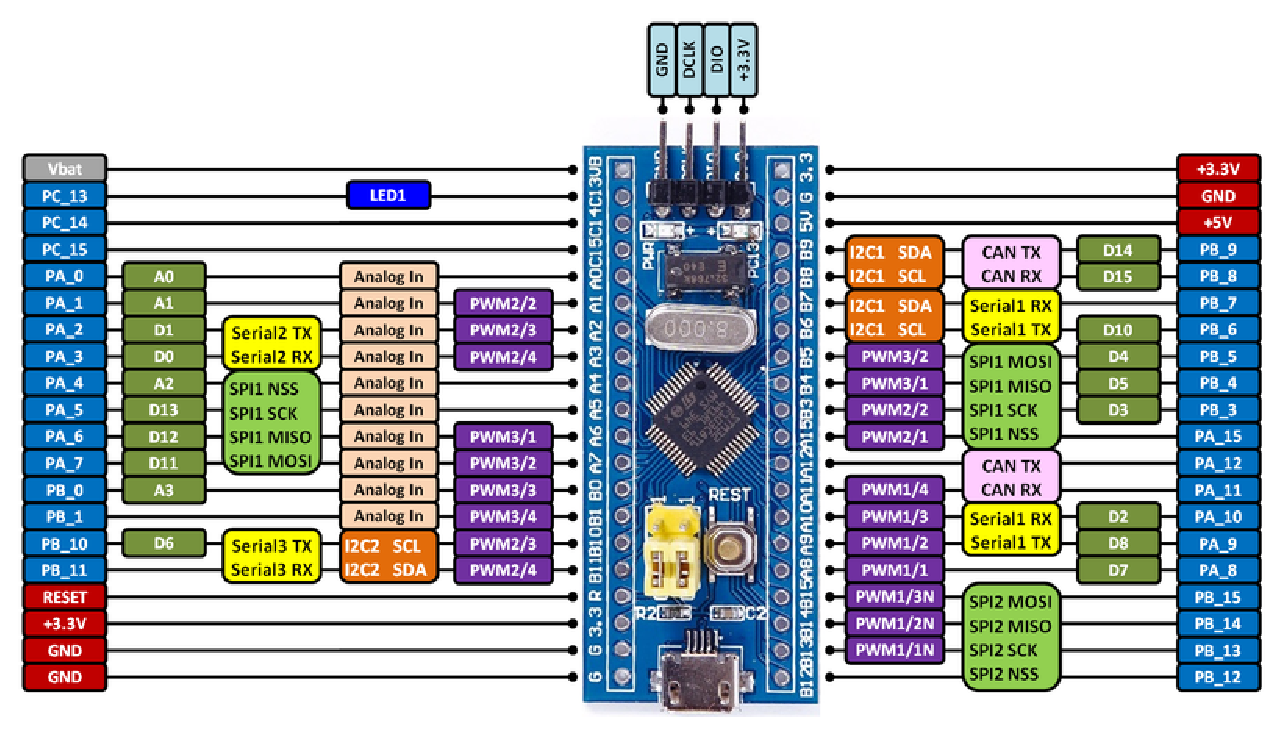
\includegraphics[width=\columnwidth]{./stm32/sevenseg/figs/stm_blue.eps}
\end{center}
\caption{Pin Connections of STM-32}
\label{fig:stm_blue}
\end{figure}
%
\begin{table}
\begin{center}
\input{./stm32/sevenseg/figs/stm_ssd}
\end{center}
\caption{STM-32 and Seven Segment Display Connections}
\label{table:stm_ssd}
\end{table}

\subsection{Software}
%
\item Before flashing code to STM32 set the STM32 board to Programming mode as shown in Fig. \ref{fig:programming_mode}, then change the mode to Operating mode as shown in Fig. \ref{fig:programming_mode} after flashing the code inorder to run your program from main memory.
\item Execute the following code 
\begin{lstlisting}
cd stm32/sevenseg/codes/sevenseg_example.c
\end{lstlisting}

%\begin{problem}
%	Connect the STM32 to the Raspberry Pi according to the \href{https://github.com/gadepall/EE4013/blob/master/setup/rpi/gvv_stm32_setup.pdf}{\url{instructions }} in
%\begin{lstlisting}
%https://github.com/gadepall/EE4013/blob/master/setup/rpi/gvv_stm32_setup.pdf
%\end{lstlisting}	
%\end{problem}
%\section{Display Control with STM32}
%
%\begin{problem}
%Follow the \href{https://github.com/gadepall/EE4013/blob/master/setup/tinker/gvv_stm32_tinker_setup.pdf}{\url{instructions }} in
%\begin{lstlisting}
%https://github.com/gadepall/EE4013/blob/master/setup/tinker/gvv_stm32_tinker_setup.pdf
%\end{lstlisting}
%to clone the \href{https://github.com/gadepall/EE4013/blob/master/setup/tinker/gvv_stm32_tinker_setup.pdf}{\url{repository }}
%\begin{lstlisting}[language=bash, frame=single, breaklines]
%https://github.com/gadepall/STM32F103C8T6
%\end{lstlisting}
%\end{problem}
%
%Fig. \ref{fig:sevenseg12} explains how to get decimal digits using the seven segment display. 
%\begin{problem}
%In the STM32F103C8T6 directory,
%\begin{lstlisting}
%cp sevenseg.c main.c
%\end{lstlisting}
%Generate the number 0 by executing \textbf{main.c} and flashing to the STM32. 
%\end{problem}	
%
%\begin{figure}[!h]
%\begin{center}
%\resizebox {0.8\columnwidth} {!} {
%\input{./figs/sevenseg12.tex}
%}
%\end{center}
%\caption{}
%\label{fig:sevenseg12}
%\end{figure}
%

\item Explain the process of generating the number 0 using the following instruction.
\begin{lstlisting}
GPIOB->ODR = 0xFC08;
\end{lstlisting}
\solution ODR is the Output Data Register, which is used to write outputs to the GPIO pins. The 16 bit number 0xFC08 on the RHS represents the pin configuration for the pins of port B of STM32F103C8T6, which are numbered PB15-PB0 in that order.  See Table \ref{table:stm_ssd}.
\\
\item Repeat the above exercise to generate the numbers 1-9 on the display.
\item The previous instructions set the bits in the unused ports PB15-PB10 and PB2-PB0. This may be undesirable in some cases. Generate 0 by not disturbing 
the unused pins.
\\
\solution The following instructions help accomplish this. The first instruction resets PB4-PB9.  The second instruction sets the PB3 pin. The other pins are
undisturbed.
\begin{lstlisting}
GPIOB->BRR = (1<<4)|(1<<5)|(1<<6)|(1<<7)|(1<<8)|(1<<9); // (Led ON)		
GPIOB->BSRR = (1<<3); // (Led OFF)					
\end{lstlisting}
%\section{Manual Display Control}
%\input{./chapters/chapter1}
%
\item Write a program to take a 4-bit BCD as input from hardware (GND or VDD) and show the next number on the seven segment display.
\\
\solution The following program takes 4 bits as input from pins PB12-PB15 and displays the output on a seven segment display. The next number
can be displayed by slightly modifying the code.
\begin{lstlisting}
cd codes/bin2dec_example.c
\end{lstlisting}
\end{enumerate}

\chapter{7447}
\iffalse
\documentclass[journal,12pt,twocolumn]{IEEEtran}
%
\usepackage{setspace}
\usepackage{gensymb}
%\doublespacing
\singlespacing

%\usepackage{graphicx}
%\usepackage{amssymb}
%\usepackage{relsize}
\usepackage[cmex10]{amsmath}
\usepackage{siunitx}
%\usepackage{amsthm}
%\interdisplaylinepenalty=2500
%\savesymbol{iint}
%\usepackage{txfonts}
%\restoresymbol{TXF}{iint}
%\usepackage{wasysym}
\usepackage{amsthm}
%\usepackage{iithtlc}
\usepackage{mathrsfs}
\usepackage{txfonts}
\usepackage{stfloats}
\usepackage{steinmetz}
\usepackage{supertabular}
%\usepackage{bm}
\usepackage{cite}
\usepackage{cases}
\usepackage{subfig}
%\usepackage{xtab}
\usepackage{longtable}
\usepackage{multirow}
%\usepackage{algorithm}
%\usepackage{algpseudocode}
\usepackage{enumitem}
\usepackage{mathtools}
\usepackage{tikz}
\usepackage{circuitikz}
\usepackage{verbatim}
\usepackage{tfrupee}
\usepackage[breaklinks=true]{hyperref}
%\usepackage{stmaryrd}
\usepackage{tkz-euclide} % loads  TikZ and tkz-base
%\usetkzobj{all}
\usetikzlibrary{calc,math}
\usetikzlibrary{fadings}
\usepackage{listings}
    \usepackage{color}                                            %%
    \usepackage{array}                                            %%
    \usepackage{longtable}                                        %%
    \usepackage{calc}                                             %%
    \usepackage{multirow}                                         %%
    \usepackage{hhline}                                           %%
    \usepackage{ifthen}                                           %%
  %optionally (for landscape tables embedded in another document): %%
    \usepackage{lscape}     
\usepackage{multicol}
\usepackage{chngcntr}
\usepackage{blkarray}
\usepackage{karnaugh-map}
\usepackage{fontspec}
\usepackage[intoc]{nomencl}
\makenomenclature

%\usetikzlibrary{arrows, shapes.gates.logic.US, calc}
\usetikzlibrary{arrows,shapes.gates.logic.US,shapes.gates.logic.IEC,calc}
\setmainfont{Sanskrit_2003.ttf}
%\setmainfont{Nakula.ttf}
%\setmainfont{Lohit-Devanagari.ttf}


%\usepackage{enumerate}

%\usepackage{wasysym}
%\newcounter{MYtempeqncnt}
\DeclareMathOperator*{\Res}{Res}
%\renewcommand{\baselinestretch}{2}
\renewcommand\thesection{\arabic{section}}
\renewcommand\thesubsection{\thesection.\arabic{subsection}}
\renewcommand\thesubsubsection{\thesubsection.\arabic{subsubsection}}

\renewcommand\thesectiondis{\arabic{section}}
\renewcommand\thesubsectiondis{\thesectiondis.\arabic{subsection}}
\renewcommand\thesubsubsectiondis{\thesubsectiondis.\arabic{subsubsection}}

% correct bad hyphenation here
\hyphenation{op-tical net-works semi-conduc-tor}
\def\inputGnumericTable{}                                 %%


\lstset{
%language=shell,
%language = Prolog,
frame=single, 
breaklines=true,
%showstringspaces=false,
columns=fullflexible
literate = {-}{-}1
}
%\lstset{
%language=tex,
%frame=single, 
%breaklines=true
%}

\begin{document}
%


\newtheorem{theorem}{Theorem}[section]
\newtheorem{problem}{Problem}
\newtheorem{proposition}{Proposition}[section]
\newtheorem{lemma}{Lemma}[section]
\newtheorem{corollary}[theorem]{Corollary}
\newtheorem{example}{Example}[section]
\newtheorem{definition}[problem]{Definition}
%\newtheorem{thm}{Theorem}[section] 
%\newtheorem{defn}[thm]{Definition}
%\newtheorem{algorithm}{Algorithm}[section]
%\newtheorem{cor}{Corollary}
\newcommand{\BEQA}{\begin{eqnarray}}
\newcommand{\EEQA}{\end{eqnarray}}
\newcommand{\define}{\stackrel{\triangle}{=}}

\bibliographystyle{IEEEtran}
%\bibliographystyle{ieeetr}


\providecommand{\mbf}{\mathbf}
\providecommand{\pr}[1]{\ensuremath{\Pr\left(#1\right)}}
\providecommand{\qfunc}[1]{\ensuremath{Q\left(#1\right)}}
\providecommand{\sbrak}[1]{\ensuremath{{}\left[#1\right]}}
\providecommand{\lsbrak}[1]{\ensuremath{{}\left[#1\right.}}
\providecommand{\rsbrak}[1]{\ensuremath{{}\left.#1\right]}}
\providecommand{\brak}[1]{\ensuremath{\left(#1\right)}}
\providecommand{\lbrak}[1]{\ensuremath{\left(#1\right.}}
\providecommand{\rbrak}[1]{\ensuremath{\left.#1\right)}}
\providecommand{\cbrak}[1]{\ensuremath{\left\{#1\right\}}}
\providecommand{\lcbrak}[1]{\ensuremath{\left\{#1\right.}}
\providecommand{\rcbrak}[1]{\ensuremath{\left.#1\right\}}}
\providecommand{\ceil}[1]{\left \lceil #1 \right \rceil }
\theoremstyle{remark}
\newtheorem{rem}{Remark}
\newcommand{\sgn}{\mathop{\mathrm{sgn}}}
\providecommand{\abs}[1]{\left\vert#1\right\vert}
\providecommand{\res}[1]{\Res\displaylimits_{#1}} 
\providecommand{\norm}[1]{\left\lVert#1\right\rVert}
%\providecommand{\norm}[1]{\lVert#1\rVert}
\providecommand{\mtx}[1]{\mathbf{#1}}
\providecommand{\mean}[1]{E\left[ #1 \right]}
\providecommand{\fourier}{\overset{\mathcal{F}}{ \rightleftharpoons}}
%\providecommand{\hilbert}{\overset{\mathcal{H}}{ \rightleftharpoons}}
\providecommand{\system}{\overset{\mathcal{H}}{ \longleftrightarrow}}
	%\newcommand{\solution}[2]{\textbf{Solution:}{#1}}
\newcommand{\solution}{\noindent \textbf{Solution: }}
\newcommand{\cosec}{\,\text{cosec}\,}
\providecommand{\dec}[2]{\ensuremath{\overset{#1}{\underset{#2}{\gtrless}}}}
\newcommand{\myvec}[1]{\ensuremath{\begin{pmatrix}#1\end{pmatrix}}}
\newcommand{\mydet}[1]{\ensuremath{\begin{vmatrix}#1\end{vmatrix}}}
%\numberwithin{equation}{section}
\numberwithin{equation}{subsection}
%\numberwithin{problem}{section}
%\numberwithin{definition}{section}
\makeatletter
\@addtoreset{figure}{problem}
\makeatother

\let\StandardTheFigure\thefigure
\let\vec\mathbf
%\renewcommand{\thefigure}{\theproblem.\arabic{figure}}
%\renewcommand{\thefigure}{\theproblem}
\renewcommand{\thefigure}{\thesection}
%\setlist[enumerate,1]{before=\renewcommand\theequation{\theenumi.\arabic{equation}}
%\counterwithin{equation}{enumi}


%\renewcommand{\theequation}{\arabic{subsection}.\arabic{equation}}

\def\putbox#1#2#3{\makebox[0in][l]{\makebox[#1][l]{}\raisebox{\baselineskip}[0in][0in]{\raisebox{#2}[0in][0in]{#3}}}}
     \def\rightbox#1{\makebox[0in][r]{#1}}
     \def\centbox#1{\makebox[0in]{#1}}
     \def\topbox#1{\raisebox{-\baselineskip}[0in][0in]{#1}}
     \def\midbox#1{\raisebox{-0.5\baselineskip}[0in][0in]{#1}}

\vspace{3cm}

\title{
%	\logo{
Digital Design through Vaman
%	}
}
\author{ G. V. V. Sharma $^{*}$% <-this % stops a space
	\thanks{*The author is with the Department of Electrical Engineering, IIT Hyderabad, 502285, India. email: gadepall@ee.iith.ac.in.  All material in this document is released under GNU GPL.  Free to use for anything.}
	
}	
%\title{
%	\logo{Matrix Analysis through Octave}{\begin{center}\includegraphics[scale=.24]{tlc}\end{center}}{}{HAMDSP}
%}


% paper title
% can use linebreaks \\ within to get better formatting as desired
%\title{Matrix Analysis through Octave}
%
%
% author names and IEEE memberships
% note positions of commas and nonbreaking spaces ( ~ ) LaTeX will not break
% a structure at a ~ so this keeps an author's name from being broken across
% two lines.
% use \thanks{} to gain access to the first footnote area
% a separate \thanks must be used for each paragraph as LaTeX2e's \thanks
% was not built to handle multiple paragraphs
%

%\author{<-this % stops a space
%\thanks{}}
%}
% note the % following the last \IEEEmembership and also \thanks - 
% these prevent an unwanted space from occurring between the last author name
% and the end of the author line. i.e., if you had this:
% 
% \author{....lastname \thanks{...} \thanks{...} }
%                     ^------------^------------^----Do not want these spaces!
%
% a space would be appended to the last name and could cause every name on that
% line to be shifted left slightly. This is one of those "LaTeX things". For
% instance, "\textbf{A} \textbf{B}" will typeset as "A B" not "AB". To get
% "AB" then you have to do: "\textbf{A}\textbf{B}"
% \thanks is no different in this regard, so shield the last } of each \thanks
% that ends a line with a % and do not let a space in before the next \thanks.
% Spaces after \IEEEmembership other than the last one are OK (and needed) as
% you are supposed to have spaces between the names. For what it is worth,
% this is a minor point as most people would not even notice if the said evil
% space somehow managed to creep in.



% The paper headers
%\markboth{Journal of \LaTeX\ Class Files,~Vol.~6, No.~1, January~2007}%
%{Shell \MakeLowercase{\textit{et al.}}: Bare Demo of IEEEtran.cls for Journals}
% The only time the second header will appear is for the odd numbered pages
% after the title page when using the twoside option.
% 
% *** Note that you probably will NOT want to include the author's ***
% *** name in the headers of peer review papers.                   ***
% You can use \ifCLASSOPTIONpeerreview for conditional compilation here if
% you desire.




% If you want to put a publisher's ID mark on the page you can do it like
% this:
%\IEEEpubid{0000--0000/00\$00.00~\copyright~2007 IEEE}
% Remember, if you use this you must call \IEEEpubidadjcol in the second
% column for its text to clear the IEEEpubid mark.



% make the title area
\maketitle

\newpage

\tableofcontents


\bigskip

\renewcommand{\thefigure}{\theenumi}
\renewcommand{\thetable}{\theenumi}
%\renewcommand{\abstractname}{सार}
%\renewcommand{\nomname}{नामकरण}
%\renewcommand{\solution}{हल: }
%\renewcommand{\figurename}{आकृति.}
%\renewcommand{\tablename}{सारणी.}
%\renewcommand{\theequation}{\theenumi}

%\begin{abstract}
%%\boldmath
%In this letter, an algorithm for evaluating the exact analytical bit error rate  (BER)  for the piecewise linear (PL) combiner for  multiple relays is presented. Previous results were available only for upto three relays. The algorithm is unique in the sense that  the actual mathematical expressions, that are prohibitively large, need not be explicitly obtained. The diversity gain due to multiple relays is shown through plots of the analytical BER, well supported by simulations. 
%
%\end{abstract}
% IEEEtran.cls defaults to using nonbold math in the Abstract.
% This preserves the distinction between vectors and scalars. However,
% if the journal you are submitting to favors bold math in the abstract,
% then you can use LaTeX's standard command \boldmath at the very start
% of the abstract to achieve this. Many IEEE journals frown on math
% in the abstract anyway.

% Note that keywords are not normally used for peerreview papers.
%\begin{IEEEkeywords}
%Cooperative diversity, decode and forward, piecewise linear
%\end{IEEEkeywords}



% For peer review papers, you can put extra information on the cover
% page as needed:
% \ifCLASSOPTIONpeerreview
% \begin{center} \bfseries EDICS Category: 3-BBND \end{center}
% \fi
%
% For peerreview papers, this IEEEtran command inserts a page break and
% creates the second title. It will be ignored for other modes.
%\IEEEpeerreviewmaketitle
\fi

\begin{abstract}
The objective of this manual is to introduce beginners to arm embedded programming by powering a seven segment display.
\end{abstract}
\subsection{Components}
\renewcommand{\theequation}{\theenumi}
\renewcommand{\thefigure}{\theenumi}
\begin{enumerate}[label=\thesubsection.\arabic*.,ref=\thesubsection.\theenumi]
\numberwithin{equation}{enumi}
\numberwithin{figure}{enumi}
\numberwithin{table}{enumi}
\item The necessary components for this manual are listed in Table \ref{tabel:stm32/sevenseg/components}.
\begin{table}[!ht]
\begin{center}
\input{./stm32/sevenseg/figs/components.tex}
\end{center}
\caption{Components}
\label{tabel:stm32/sevenseg/components}
\end{table}
\subsection{Hardware}

%\subsection{Seven Segment Display}
%The breadboard can be divided into 5 segments.  In each of the green segements, the pins are internally connected so as to have the same voltage.  Similarly, in the central segments, the pins in each column  are internally connected in the same fashion as the blue columns. 

%\begin{problem}
%	Plug the display to the breadboard in Fig. \ref{fig:breadboard}
%\end{problem}
%\begin{figure}[!h]
%\begin{center}
%\includegraphics[width=\columnwidth]{./figs/breadboard}
%\end{center}
%\caption{}
%\label{fig:breadboard}
%\end{figure}
\item The seven segment display in Fig. \ref{fig:sevenseg} has eight pins, $a, b, c, d, e, f, g$ and $dot$ that take an active LOW input, i.e.  the LED will glow only if the input is connected to ground.  Each of these pins is connected to an LED segment.  The $dot$ pin is  reserved for the $\cdot$ LED.  

%
%\begin{center}
	%\includegraphics[scale=1]{sevenseg}
%\end{center}


\item Connect one end of the 1K resistor to the COM pin of the display and the other end to an extreme pin of the breadboard.	
%
%
%
%\begin{figure}[!h]
%\begin{center}
%\resizebox {0.5\columnwidth} {!} {
%\input{./figs/sevenseg.tex}
%}
%\end{center}
%\caption{}
%\label{fig:sevenseg}
%\end{figure}

\item The STM32F103C8T6 micro-controller in Fig. \ref{fig:stm_blue} has two ground pins, few analog input pins and few digital pins that can be used for both input as well as output. It has one Vcc (3.3V) pin that can generate 3.3$V$.  In the following exercises, only the GND, 3.3$V$ and digital pins will be used.
%
%
\item Make the pin connections in Table \ref{table:stm_ssd} using Figs. \ref{fig:sevenseg} and \ref{fig:stm_blue}.
	
%
\begin{figure}[!h]
\begin{center}
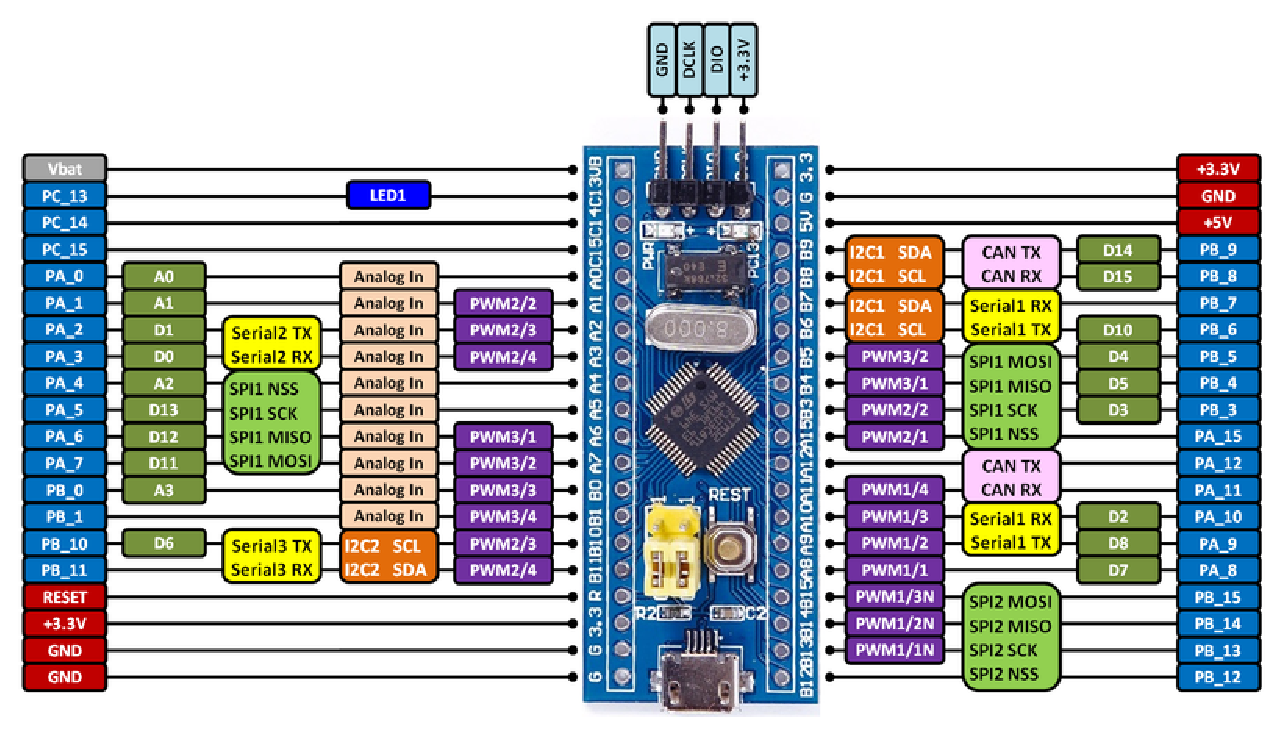
\includegraphics[width=\columnwidth]{./stm32/sevenseg/figs/stm_blue.eps}
\end{center}
\caption{Pin Connections of STM-32}
\label{fig:stm_blue}
\end{figure}
%
\begin{table}
\begin{center}
\input{./stm32/sevenseg/figs/stm_ssd}
\end{center}
\caption{STM-32 and Seven Segment Display Connections}
\label{table:stm_ssd}
\end{table}

\subsection{Software}
%
\item Before flashing code to STM32 set the STM32 board to Programming mode as shown in Fig. \ref{fig:programming_mode}, then change the mode to Operating mode as shown in Fig. \ref{fig:programming_mode} after flashing the code inorder to run your program from main memory.
\item Execute the following code 
\begin{lstlisting}
cd stm32/sevenseg/codes/sevenseg_example.c
\end{lstlisting}

%\begin{problem}
%	Connect the STM32 to the Raspberry Pi according to the \href{https://github.com/gadepall/EE4013/blob/master/setup/rpi/gvv_stm32_setup.pdf}{\url{instructions }} in
%\begin{lstlisting}
%https://github.com/gadepall/EE4013/blob/master/setup/rpi/gvv_stm32_setup.pdf
%\end{lstlisting}	
%\end{problem}
%\section{Display Control with STM32}
%
%\begin{problem}
%Follow the \href{https://github.com/gadepall/EE4013/blob/master/setup/tinker/gvv_stm32_tinker_setup.pdf}{\url{instructions }} in
%\begin{lstlisting}
%https://github.com/gadepall/EE4013/blob/master/setup/tinker/gvv_stm32_tinker_setup.pdf
%\end{lstlisting}
%to clone the \href{https://github.com/gadepall/EE4013/blob/master/setup/tinker/gvv_stm32_tinker_setup.pdf}{\url{repository }}
%\begin{lstlisting}[language=bash, frame=single, breaklines]
%https://github.com/gadepall/STM32F103C8T6
%\end{lstlisting}
%\end{problem}
%
%Fig. \ref{fig:sevenseg12} explains how to get decimal digits using the seven segment display. 
%\begin{problem}
%In the STM32F103C8T6 directory,
%\begin{lstlisting}
%cp sevenseg.c main.c
%\end{lstlisting}
%Generate the number 0 by executing \textbf{main.c} and flashing to the STM32. 
%\end{problem}	
%
%\begin{figure}[!h]
%\begin{center}
%\resizebox {0.8\columnwidth} {!} {
%\input{./figs/sevenseg12.tex}
%}
%\end{center}
%\caption{}
%\label{fig:sevenseg12}
%\end{figure}
%

\item Explain the process of generating the number 0 using the following instruction.
\begin{lstlisting}
GPIOB->ODR = 0xFC08;
\end{lstlisting}
\solution ODR is the Output Data Register, which is used to write outputs to the GPIO pins. The 16 bit number 0xFC08 on the RHS represents the pin configuration for the pins of port B of STM32F103C8T6, which are numbered PB15-PB0 in that order.  See Table \ref{table:stm_ssd}.
\\
\item Repeat the above exercise to generate the numbers 1-9 on the display.
\item The previous instructions set the bits in the unused ports PB15-PB10 and PB2-PB0. This may be undesirable in some cases. Generate 0 by not disturbing 
the unused pins.
\\
\solution The following instructions help accomplish this. The first instruction resets PB4-PB9.  The second instruction sets the PB3 pin. The other pins are
undisturbed.
\begin{lstlisting}
GPIOB->BRR = (1<<4)|(1<<5)|(1<<6)|(1<<7)|(1<<8)|(1<<9); // (Led ON)		
GPIOB->BSRR = (1<<3); // (Led OFF)					
\end{lstlisting}
%\section{Manual Display Control}
%\input{./chapters/chapter1}
%
\item Write a program to take a 4-bit BCD as input from hardware (GND or VDD) and show the next number on the seven segment display.
\\
\solution The following program takes 4 bits as input from pins PB12-PB15 and displays the output on a seven segment display. The next number
can be displayed by slightly modifying the code.
\begin{lstlisting}
cd codes/bin2dec_example.c
\end{lstlisting}
\end{enumerate}

\section{Problems}
\begin{enumerate}
\item Obtain the Boolean Expression for the Logic circuit shown below
\label{prob:2013/c/6/b}
\hfill (CBSE 2013)
	\usetikzlibrary{circuits.logic.IEC,calc}

	   \begin{circuitikz} \draw
(0,2) node[or port]  (myor1) {}
(0,0) node[and port] (myand) {}
(2,1) node[or port] (myor2) {}
(myor1.out) -- (myor2.in 1)
(myand.out) -- (myor2.in 2);

\node[left] at (myor1.in 1) {\(X\)};
\node[left] at (myor1.in 2) {\(Y\)};
\node[left] at (myor1.in 1)[ocirc] {};
\node[left] at (myand.in 2) [ocirc] {};
\node[left] at (myand.in 1) {\(Y\)};
\node[left] at (myand.in 2) {\(Z\)};
\node[right] at (myor1.out) {};
\node[right] at (myand.out) {};

\node[right] at (myor2.out) {F};
\end{circuitikz}
\item Verify the Boolean Expression 
\label{prob:2013/c/6/a}
\hfill (CBSE 2013)
		\begin{align}
\label{eq:2013/c/6/a}
	               A+C=A+A'C+BC
		\end{align}
\item Draw the Logic Circuit for the following Boolean Expression 
\label{prob:2015-1/c/6/b}
\hfill (CBSE 2015)
		\begin{align}
\label{eq:2015-1/c/6/b}
f(x,y,z,w) = (x'+y)z + w'
		\end{align}
\item Verify the following
\label{prob:2015-1/c/6/a}
\hfill (CBSE 2015)
		\begin{align}
\label{eq:2015-1/c/6/a}
U' + V = U'V' + U'V+UV
		\end{align}
\item Draw the Logic Circuit for the given Boolean Expression
\label{prob:2015/c/6/b}
\hfill (CBSE 2015)
		\begin{align}
\label{eq:2015/c/6/b}
(U + V')W' + Z
		\end{align}
\item 
Verify the following using Boolean Laws
\label{prob:2015/c/6/a}
\hfill (CBSE 2015)
		\begin{align}
\label{eq:2015/c/6/a}
X+Y' = XY+XY'+X'Y'
		\end{align}
\item 
\label{prob:2016/c/6/b}
Write the Boolean Expression for the result of the Logic Circuit as shown in Fig.  
\ref{fig:2016/c/6/b}
\hfill (CBSE 2016)
\begin{figure}
\centering
\includegraphics[width=\columnwidth]{figs/cbse-2016.jpg}
\caption{}
\label{fig:2016/c/6/b}
\end{figure}
\item Draw the logic circuit of the following Boolean Expression using only NAND Gates.
\hfill (CBSE 2017)
\label{prob:2017-1/c/6/b}
		\begin{align}
\label{eq:2017-1/c/6/b}
 XY + YZ
		\end{align}
\item Draw the Logic Circuit of the following Boolean Expression using only NOR Gates  
\hfill (CBSE 2017)
\label{prob:2017/c/6/b}
      \begin{align}
      (A+B)(C+D)
      \end{align}
\item Draw the Logic Circuit of the following Boolean Expression\hfill (CBSE 2018)
\begin{equation} 
(U'+V)(V'+W')
\end{equation}
\label{prob:2018/c/6/b}
\item Derive a Canonical POS expression for a Boolean function F, represented by 
Table \ref{tab:2019/c/6/c}\hfill (CBSE 2019)
\label{prob:2019/c/6/c}
\begin{table}[H]
\centering
\begin{tabular}{|l|l|l|c|}
	\hline
	X&Y&Z&F(X,Y,Z)\\
	\hline
	0&0&0&1\\
	0&0&1&0\\
	0&1&0&1\\
	0&1&1&0\\
	1&0&0&1\\
	1&0&1&1\\
	1&1&0&0\\
	1&1&1&0\\
	\hline
\end{tabular}
\caption{}
\label{tab:2019/c/6/c}
\end{table}
\item For the logic circuit shown in Fig.\ref{fig:2000/gate/ec/2/7}, find the simplified Boolean expression for the output. 
\label{prob:2000/gate/ec/2/7}
\hfill (GATE EC 2000)
\begin{figure}[H]
    \centering
    \includegraphics[width=\columnwidth]{figs/2000-gate-ec-2-7.jpg}
    \caption{}
\label{fig:2000/gate/ec/2/7}
\end{figure}
\item 
Obtain the Boolean Expression for the Logic circuit shown below
\label{prob:1993/gate/ec/4/8}
\hfill (GATE EC 1993)
	  	
	   \begin{circuitikz} \draw
(0,2) node[nand port] (mynand1) {}
(2,3) node[nand port] (mynand2) {}
(0,0) node[nand port] (mynand) {}
(2,-1) node[nand port] (mynand3) {}
(2,1) node[or port] (myor1) {}
(4,1) node[or port,number inputs =3] (myor2) {}
(mynand1.out) -- (myor1.in 1)
(mynand.out) -- (myor1.in 2)
(mynand2.out) -- (myor2.in 1)
(mynand3.out) -- (myor2.in 3)
(myor1.out) -- (myor2.in 2);
\node[left] at (mynand1.in 1) {\(A\)};
\node[left] at (mynand1.in 2) {\(B\)};
\node[left] at (mynand2.in 1) {\(A\)};
\node[left] at (mynand2.in 2) {\(A\)};
\node[left] at (mynand3.in 1) {\(C\)};
\node[left] at (mynand3.in 2) {\(C\)};
\node[left] at (mynand1.in 1)[ocirc] {};
\node[left] at (mynand.in 2) [ocirc] {};
\node[left] at (mynand.in 1) {\(B\)};
\node[left] at (mynand.in 2) {\(C\)};
\node[right] at (mynand1.out) {};
\node[right] at (mynand.out) {};
\node[right] at (mynand2.out) {};
\node[right] at (mynand3.out) {};
\node[right] at (myor2.out) {\(Y\)};
\end{circuitikz}
%
\item Implement Table
\ref{tab:1993/gate/ec/6/13}
using XNOR logic.
\label{prob:1993/gate/ec/6/13}
\hfill (GATE EC 1993)
\begin{table}[H]
	\centering
	\begin{tabular}{|c|c|c|}
		\hline
		\textbf{A}&\textbf{B}&\textbf{Y}\\
		\hline
		0&0&1\\
		\hline
		0&1&0\\
		\hline
		1&0&0\\
		\hline
		1&1&1\\   
		\hline 
	\end{tabular}
	\caption{}
\label{tab:1993/gate/ec/6/13}
\end{table}
\item 
\label{prob:1999-gate-ec-2-11}
For a binary half-sub-tractor having two inputs A and B, find the correct set of logical expressions for the outputs D (=A minus B) and X (=borrow).
\hfill (GATE EC 1999)
%
\item 
\label{prob:2007-gate-ec-43}
Find $X$ in the following circuit in Fig.
\ref{fig:2007-gate-ec-43}
\hfill (GATE EC 2007)
\begin{figure}[H]
\centering
	\includegraphics[width=1\columnwidth]{figs/2007-gate-ec-43.png}
\caption{}
\label{fig:2007-gate-ec-43}
\end{figure}
\item 
\label{prob:2007-gate-in-10}
      A logic circuit implements the boolean function F=X'.Y+X.Y'.Z'. It is found that the input combination X=Y=1 can never occur. Taking this into account, find a simplified expression for F. 
\hfill (GATE IN 2007)
\item 
\label{prob:2010-gate-ec-39}
Find the Boolean logic realised by the following circuit in Fig.
\ref{fig:2010-gate-ec-39}
\hfill (GATE EC 2010)
\begin{figure}[H]
\centering
	\includegraphics[width=1\columnwidth]{figs/2010-gate-ec-39.png}
\caption{}
\label{fig:2010-gate-ec-39}
\end{figure}
\item 
\label{prob:2011-gate-ec-20}
Find the logic function implemented by the circuit given below 
in Fig.
\ref{fig:2011-gate-ec-20}
\hfill (GATE EC 2011)
\begin{figure}[H]
\centering
	\includegraphics[width=\columnwidth]{figs/2011-gate-ec-20.png}
\caption{}
\label{fig:2011-gate-ec-20}
\end{figure}
\item
\label{prob:2016/gate/in/19}
Find F in the Digital Circuit given in the figure below
in Fig. \ref{fig:2016/gate/in/19}.
\hfill (GATE IN 2016)
\begin{figure}[H]
	\centering
\begin{tikzpicture}
 

 
% Logic ports
\node[nand port] (a) at (2,1){};
\node[nand port] (b) at (2,4){};
\node[nand port] (c) at (4,0){};
\node[nand port] (d) at (6,3){};

 
% Connection

 
\draw (a.in 2) -| (b.in 2);
\draw (b.out) -| (d.in 1);
 
\draw (a.out) -|  (c.in 1);
\draw (c.out) -| (d.in 2);
\draw (d.out) -- ++(1,0) node[near end,above]{F};
 
\draw (b.in 1) -- ++(-1.5,0)node[left](In1){X};
\draw (b.in 2) -- ++(-1.5,0)node[left](In3){Y};
\draw (c.in 2) -- ++(-1.5,0)node[left](In3){Z};
% Jump crossing element
1
\end{tikzpicture}
	\caption{}
\label{fig:2016/gate/in/19}
\end{figure}


\item 
\label{prob:2017-gate-ec-16}
Find the logic function implemented by the circuit given below 
in Fig.
\ref{fig:2017-gate-ec-16}
\hfill (GATE EC 2017)
\begin{figure}[H]
\centering
	\includegraphics[width=\columnwidth]{figs/2017-gate-ec-16.png}
\caption{}
\label{fig:2017-gate-ec-16}
\end{figure}
\item 
\label{prob:2018-gate-ec-31}
Find the logic function implemented by the circuit given below 
in Fig.
\ref{fig:2018-gate-ec-31}
\hfill (GATE EC 2018)
\begin{figure}[H]
\centering
	\includegraphics[width=\columnwidth]{figs/2018-gate-ec-31.png}
\caption{}
\label{fig:2018-gate-ec-31}
\end{figure}
\item 
\label{prob:2018-gate-ee-14}
Find the logic function implemented by the circuit given below 
in Fig.
\ref{fig:2018-gate-ee-14}
\hfill (GATE EE 2018)
\begin{figure}[H]
\centering
	\includegraphics[width=\columnwidth]{figs/2018-gate-ee-14.png}
\caption{}
\label{fig:2018-gate-ee-14}
\end{figure}
\item 
\label{prob:2019-gate-ee-36}
Find the logic function implemented by the circuit given below 
in Fig.
\ref{fig:2019-gate-ee-36}
\hfill (GATE EE 2019)
\begin{figure}[H]
\centering
	\includegraphics[width=\columnwidth]{figs/2019-gate-ee-36.png}
\caption{}
\label{fig:2019-gate-ee-36}
\end{figure}
\item 
\label{prob:2018-gate-CS-4}		
Let $\oplus$ and $\odot$ denote the Exclusive OR and Exclusive NOR operations, respectively.Which one of the following is NOT CORRECT ?
\ref{prob:2018-gate-CS-4}
\hfill (GATE CS 2018)
\begin{samepage}
\begin{enumerate}[label=(\Alph*)]
    \item $\overline{P\oplus Q}$ = $ P \odot Q $
    \item $\overline{P} \oplus Q$ = $ P \odot Q $
    \item $\overline{P} \oplus \overline{Q}$ = $ P \oplus Q $
    \item $(P \oplus \overline{P}) \oplus Q$ = $(P \odot \overline{P}) \odot \overline{Q}$
\end{enumerate}
\end{samepage}

\item A Boolean digital circuit is composed using two 4-input multiplexers $(M1 and M2)$ and one 2-input multiplexer $(M3)$ as shown in the figure. $X0$–$X7$ are the inputs of the multiplexers $M1$ and $M2$ and could be connected to either $0$ or $1$. The select lines of the multiplexers are connected to Boolean variables $A$, $B$ and $C$ as shown.\hfill(GATE CS2023,44)

\begin{figure}[H]
    \centering
        \includegraphics[width=\columnwidth]{figs/Multiplexer.png}
    \caption{Digital Circuit}
    \label{fig:Multiplexer}
\end{figure}

Which one of the following set of values of $(X0, X1, X2, X3, X4, X5, X6, X7)$ will realise the Boolean function 
$\overline{A} + \overline{A}.\overline{C}+A.\overline{B}.C $ ?
 \begin{enumerate}
     \item (1, 1, 0, 0, 1, 1, 1, 0)
     \item (1, 1, 0, 0, 1, 1, 0, 1)
     \item (1, 1, 0, 1, 1, 1, 0, 0)
     \item (0, 0, 1, 1, 0, 1, 1, 1)
 \end{enumerate}
\item For the given digital circuit, $A = B = 1$. Assume that AND, OR, and NOT gates have propagation delays of $10\mathrm{ns}$,$10\mathrm{ns}$, and $5\mathrm{ns}$ respectively. All lines have zero
propagation delay. Given that $C = 1$ when the circuit is turned on, the frequency of steady-state oscillation of the output $Y$  is  \rule{30pt}{1pt}.
\hfill (GATE IN 2023)
\begin{figure}[H]
        \centering  
        
        \includegraphics[width=\columnwidth]{figs/gate.png}
        \caption{Image}
	\label{fig:Image}
        
\end{figure}
    \begin{enumerate}
        \item $20 \mathrm{MHz}$
        \item $15 \mathrm{MHz}$
        \item $40 \mathrm{MHz}$
        \item $50 \mathrm{MHz}$
    \end{enumerate}
\item Select the Boolean function(s) equivalent to $x + yz$, where $x,y$, and $z$ are Boolean variables, and + denotes logical OR  operation.\hfill(GATE EC 2022)
	\begin{enumerate}[label=(\Alph*)]
		\item $x + z + {xy}$
		\item ${(x + y)}{(x + z)}$
		\item $x + {xy} + {yz}$
		\item $x + {xz} + {xy}$
	\end{enumerate}
 \item Which one of the following options is CORRECT for the given circuit ?\hfill(GATE PHYSICS 2023)
		\begin{figure}[H]
			\centering
			\includegraphics[width=\columnwidth]{figs/Q24.jpg}
			\caption{}
			\label{figure:xxxx}
		\end{figure}

		\begin{enumerate}[label=(\Alph*)]
		\item P = $1$, Q = $1$ ; X = $0$
		\item P = $1$, Q = $0$ ; X = $1$
		\item P = $0$, Q = $1$ ; X = $0$
		\item P = $0$, Q = $0$ ; X = $1$
	\end{enumerate}

\item In the circuit diagram shown below, the logic gates operate with a supply voltage of $1 V$. NAND and XNOR have $200$ps and $400$ps input-to-output delay, respectively.

At time $t=T.A(t)=0,B(t)=1 and Z(t)=0.$ When the inputs are changed to $A(t)=1,B(t)=0 \text{at} t=2T$, a 1 V pulse is observed at $Z$. the pulse width of the $1 V$ pulse is  ps.


\hfill{(GATE BM 2022)}

\begin{figure}[H]
\centering
\includegraphics[width=\columnwidth]{figs/bm2022.png}
\caption{}
\label{fig:GATE Digram}
\end{figure}

\begin{enumerate}
\item $100$
\item $200$
\item $400$
\item $600$
\end {enumerate}

\item 
Consider a Boolean gate (D) where the output (Y) is related to the inputs (A) and (B) as, $Y = A + B$, where + denotes logical OR operation. The Boolean inputs '0' and '1' are also available separately. Using instances of only D gates and inputs '0' and '1', (select the correct option(s)).\hfill{(GATE EC 2022)}

\begin{enumerate}
\item  NAND logic can be implemented
\item  OR logic cannot be implemented
\item  NOR logic can be implemented
\item  AND logic cannot be implemented.
\end{enumerate}

\item Let $R1$ and $R2$ be two $4$-bit registers that store numbers in $2$’s complement form.
For the operation $R1+R2$, which one of the following values of $R1$ and $R2$ gives an
arithmetic overflow?
\hfill{(GATE CS 2022)}

    \begin{enumerate}
        \item $R1 = 1011$ and $R2 = 1110$
        \item $R1 = 1100$ and $R2 = 1010$
        \item $R1 = 0011$ and $R2 = 0100$
        \item $R1 = 1001$ and $R2 = 1111$
    \end{enumerate}


\item The maximmunm clock frequeccy in MHz of a $4$-stage ripple counter, utilize flip-flops, with each flip-flop having a propagation delay of $20$ ns, is $\rule{2cm}{0.15mm}$.\\
(\textit{round off to one decimal place})
\hfill{(GATE EE 20222)}

\item The logic block shown has an output $F$ given by \rule{2cm}{0.15mm}
\hfill{(GATE IN 2021)}
\begin{figure}[H]
\centering
\includegraphics[width=\columnwidth]{figs/gatemage.jpg}
\end{figure}
\begin{enumerate}
	\item$A+B$
	\item$A.\bar{B}$
	\item$A+\bar{B}$
	\item$\bar{B}$
\end{enumerate}

\item Consider the following Boolean expression 
\begin{align*} F = (X+Y+Z)(\bar{X}+Y)(\bar{Y}+Z) \end{align*}
       
Which of the following Boolean expressions is/are equivalent to $\overline{F}$ (complement of 
 F)?
 
\hfill{(Gate CS 2021,42)}
\begin{enumerate}                                     
\item $(\bar{X}+\bar{Y}+\bar{Z})(X+\bar{Y})(Y+\bar{Z})$
\item $X\bar{Y}+\bar{Z}$
\item $(X+\bar{Z})(\bar{Y}+\bar{Z})$
\item $X\bar{Y}+Y\bar{Z}+\bar{X}\bar{Y}\bar{Z}$ 
\end{enumerate}

    \item The propagation delays of the XOR gate, AND gate and multiplexer \brak{MUX} in the circut shown in the figure are $4 ns$, $2 ns$ and $1 ns$, respectively.
    If all the inputs $P, Q, R, S$ and T are applied simultaneously and held constant, the maximum propagation delay of the circuit is
\hfill(GATE-EC2021,31)  

\begin{figure}[H]
\begin{circuitikz}
\draw (7,1)coordinate (E) -- (8,1)coordinate (F) -- (8,-1)coordinate (G) -- (7,-1)coordinate (H) -- (7,1)coordinate (E);
\draw (11,2)coordinate (I) -- (13,2)coordinate (J) -- (13,-1)coordinate (K) -- (11,-1)coordinate (L) -- (11,2)coordinate (I);
 \draw ($(J)!0.5!(K)$)--++(0:2)node[right]{$Y$};
 \draw ($(L)!0.5!(K)$)node[anchor=south]{$S0$}--++(90:-2)--++(1:-10)node[left]{$T$};
 \draw ($(H)!0.5!(G)$)node[anchor=south]{$S0$}--++(90:-2)--++(1:0)node[left]{};
\draw (4,2) node[and port] (myand1) {};
\draw (myand1.in 1) node (A1)     [anchor=east,xshift=-1cm]           {$P$}
(myand1.in 1) -- (A1);
\draw(4,-2) node[and port] (myand2) {}
(myand2.in 2) node (B2)     [anchor=east,xshift=-1cm]           {$S$};
\draw(myand2.in 2) -- (B2);
\draw (10,0) node[and port] (myand3) {};
\draw (4,0) node[xor port] (myxor) {};
\draw (myand1.in 2) node (B1)     [anchor=east,xshift=-1cm,yshift=-.7cm]  {$Q$};
\draw (B1) -- ++(1.25cm,0);
\draw (myxor.in 1) node (B1)     [anchor=east,xshift=-1cm,yshift=-1.3cm]  {$R$};
\draw (B1) -- ++(1.25cm,0);

\draw (myand1.in 2) |- (myxor.in 1);
\draw (myand2.in 1) |- (myxor.in 2);

\draw (myxor.out) |- ($(E)!0.2!(H)$)--++(0:0)node[right]{$0$};
\draw(myand1.out) |- ($(I)!0.2!(L)$)--++ (0:0)node[right]{$0$};
\draw (myand1.out) -| (myand3.in 1);
\draw(myand3.out) -| ($(I)!0.7!(L)$)--++(0:0)node[right]{$1$};
\draw ($(F)!0.6!(G)$)--++(0:0)node[right]{} -| (myand3.in 2) ;
\draw (myand2.out) |- ($(E)!0.7!(H)$)--++(0:0)node[right]{$1$};

\end{circuitikz}
~


\caption{circuit daigram} 
\label{fig:block_diagram}
\end{figure}
\begin{enumerate}

    \item $3 ns$
    \item $5 ns$
    \item $6 ns$
    \item $7 ns$
\end{enumerate}
\item  The above combination of logic gate represent the operation
 \hfill(GATE PH 2021)
	      \begin{figure}[H]
		      \centering
		                   \begin{circuitikz}
              
                  \draw (2,5) node[not port,scale=2] (not) {};
                  \draw (not.in) -- ++(-0.5,0);
                  \draw (not.out) -- ++(0.5,0) ;
                  
                
                
                \draw (7.5,3) node[or port,scale=2] (orgate) {};
                  \draw (orgate.in 1) -- ++(-0.5,0) ;
                  \draw (orgate.in 2) -- ++(-0.5,0);
                  \draw (orgate.out) -- ++(0.5,0) ;
                
                 \draw (2,1) node[not port,scale=2] (notgate) {};
                  \draw (notgate.in) -- ++(-0.5,0) ;
                  \draw (notgate.out) -- ++(0.5,0) ;
                
                \draw (notgate.out) -- ([xshift=0.5cm]notgate.out) |-(orgate.in 2);
                  
                \draw (not.out) -- ([xshift=0.5cm]not.out) |-(orgate.in 1);
                  
            \end{circuitikz}

	              \caption{combination circuit}
	      \end{figure}

	\begin{enumerate}
       \item OR
       \item NAND
       \item AND
       \item NOR
   \end{enumerate}
\item Consider the boolean Function $z\brak{a,b,c}$ from below .
		\begin{figure}[H]
			\centering
			\includegraphics[width=\columnwidth]{figs/203.png}
			\caption{circuit diagram}
		\end{figure}
		
	\hfill{(Gate CS-2020)}
	
		Which of the following minterm lists represent the circuit given above?
	\begin{enumerate}
		\item $z=\Sigma\brak{0,1,3,7}$
		\item $z=\Sigma\brak{1,4,5,6,7}$
		\item $z=\Sigma\brak{2,4,5,6,7}$
		\item $z=\Sigma\brak{2,3,5}$
	\end{enumerate}	   
\item In the latch circuit shown, the NAND gates have non-zero but unequal propagation delays. The present input condition is: $P=Q=\lq 0\rq$. If the input condition is changed simultaneously to $P=Q=\lq 1\rq$,the outputs $X$ and $Y$ are 
\begin{figure}[H]
\centering
\label{figure_1}
\begin{circuitikz}
    \draw (0,0) node[nand port] (nand1) {};
    \draw (0,-2) node[nand port] (nand2) {};
    \draw (nand1.in 1) -- ++(-0.5,0) node[left] {$P$};
    \draw (nand1.in 2) -- ++(-0.2,0) coordinate (in1);
    \draw (nand1.out) -- ++(0.1,0) coordinate (out1); 
    \draw (nand2.in 1) -- ++(-0.2,0) coordinate (in2);
    \draw (nand2.in 2) -- ++(-0.5,0) node[left] {$Q$};
    \draw (nand2.out) -- ++(0.1,0) coordinate (out2);
    \draw (out2)-- ++(0,0.5)-- ++(-2,1) |- (in1);
    \draw (out1)-- ++(0,-0.5)-- ++(-2,-1) |- (in2);
    \draw (out1) -- ++(1,0) node[above right] {X};
    \draw (out2) -- ++(1,0) node[above right] {Y};
\end{circuitikz}

\end{figure}
\begin{enumerate}
\item $X=\lq 1\rq,Y=\lq 1 \rq$
\item either $X=\lq 1\rq,Y=\lq 0\rq$ or $X=\lq 0\rq,Y=\lq 1\rq$
\item either $X=\lq 1\rq,Y=\lq 1\rq$ or $X=\lq 0\rq,Y=\lq 0\rq$
\item $X=\lq 0\rq,Y=\lq 0 \rq$
\end{enumerate}
\hfill(GATE EC 2017)

\item Consider three $4$-variable functions $f_1, f_2, $and $f_3,$ which are expressed in sum-of-minterms as \newline \quad $f_1 = \sum\brak{0,2,5,8,14}$, \quad $f_2=\sum\brak{2,3,6,8,14,15}$, \quad $f_3 = \sum\brak{2,7,11,14}$ \newline For the following circuit with one AND gate and one XOR gate, the output function $f$ can be expressed as:
	\hfill(GATE-CS2019,30)
	\begin{figure}[H]
		 \centering
			\begin{circuitikz}
    % Draw AND gate
    \draw (0,0) node[and port] (and) {AND};
    
    % Draw XOR gate
    \draw (4,-0.2) node[xor port] (xor) {XOR};
    
    % Connect AND output to XOR input
    \draw (and.out) -- (xor.in 1);
    
    % Draw input wires
    \draw (and.in 1) -- ++(-1,0) node[left] {$f_1$};
    \draw (and.in 2) -- ++(-1,0) node[left] {$f_2$};
    \draw (xor.in 2)--++(-90:2) --++(-5,0) node[left] {$f_3$};    % Draw XOR output
    \draw (xor.out) -- ++(1,0) node[right] {$f$};
\end{circuitikz}


                 \caption{Circuit Daigram}
	\end{figure}
		\begin{enumerate}
		\item $\sum\brak{7,8,11}$
		\item $\sum\brak{2,7,8,11,14}$
		\item $\sum\brak{2,14}$
		\item $\sum\brak{0,2,3,5,6,7,8,11,14,15}$
		\end{enumerate}

\item In the circuit shown, what are the values of $F$for $EN=0$ and $EN=1$,  respectively?
 \hfill(GATE-EC2019,14)  

\begin{figure}[H]
    \centering
    \begin{circuitikz}

\draw (0.5,1) node[nand port] (nand) {};
\draw (nand.in 1) -- ++(-1.7,0) node[left] {};
\draw (nand.in 2) -- ++(-2.2,0) node[left] {EN};
\draw (nand.out) -- ++(0.5,0) node[midway, above] {};
\draw (0.5,-3) node[nor port] (nor) {};
\draw (nor.in 1) node[left] {};
\draw (nor.in 2) --++(-2.2,0) node[left] {D};
\draw (nor.out) -- ++(0.5,0) node[midway, above] {};
\draw (-1.6,-1) node[rotate=270,not port] (not) {};
\draw (not.in) |-(nand.in 2);
\draw  (nor.in 1) -| (not.out);
\draw (2,1) node[pmos] (pmos) {};
\draw (2,-3) node[nmos] (nmos) {};
\draw (nand.out) -- (pmos.gate);
\draw (nor.out) -- (nmos.gate);
\draw(nand.in 1) -- ++(-1.7,0) |- (nor.in 2) -- ++(-1,0);
\draw (pmos.drain) -- (nmos.drain);
\draw (pmos.drain)--++(90:-1)--++(2:1)node[left, yshift=0.2cm]{$F$};
\draw (nmos.source) -- (nmos.source |- 0,-4) node[ground] {};
\draw(2,1.7) node[rground,yscale=-1] {};
\draw(2,2.3) node(right) {$V_{DD}$};

\end{circuitikz}


    \caption{Circuit Diagram}
\end{figure}
\begin{enumerate}
    \item $0$ and $D$
    \item $Hi-Z$ and $D$
    \item $0$ and $1$
    \item $Hi-Z$ and $\overline{D}$
\end{enumerate}
\item In the circuit shown, $A$ and $B$ are the inputs and $F$ is the output. What is the functionality of the circuit?
           \hfill(GATE-EC2019,15)
           
\begin{figure}[H]
\centering

\begin{circuitikz}
    % Draw PMOS transistors
     \draw (2,1) node [pmos] (pmos1) {};
    \draw (2,0) node [pmos,rotate=180] (pmos2) {};
    \draw (0,-2) node [nmos,rotate=180] (nmos1) {};
    \draw (4,-2) node [nmos] (nmos2) {};
    
    % connections
     \draw(pmos1.gate)  -- (nmos1.gate);
      \draw(pmos2.gate) -- (nmos2.gate);
     \draw (pmos1.drain) -- (pmos2.drain);
    \draw (nmos1.source) -- (nmos2.drain);
    \draw (nmos1.gate) --(nmos2.source);
    \draw (nmos2.gate) -- (nmos1.drain);
    \draw (pmos2.source) -- (2,-1.22);
    \draw (nmos2.drain) -- (4,-1.22) node[circ]{};
    \draw (nmos2.drain)node[anchor=east,xshift=0.45cm,yshift=-0cm] 
    {$F$};
    %%B
    \draw (nmos2.source) node[circ]{};
    \draw (nmos2.source)node[anchor=east,xshift=0.48cm,yshift=-0cm] {$B$};
    %%A
    \draw (nmos1.drain)node[circ]{};
     \draw (nmos1.drain)node[anchor=east,xshift=0cm,yshift=-0cm] {$A$};
     %%vdd
    \draw (2,1.75) node[rground,yscale=-1] {};
    \draw (2.5,1.8) node(right) {$V_{DD}$};
\end{circuitikz}


\caption{Circuit Diagram}

\end{figure}
\begin{enumerate}
\item Latch
\item XNOR
\item SRAM Cell
\item XOR
\end{enumerate}

\item In the circuit shown below, assume that the comparators are ideal and all components have zero propagation delay. In one period of the input signal $Vin=6\sin\brak{\omega t}$, the fraction of the time for which the output OUT is in logic HIGH is 
		                 \hfill(GATE-IN2019,34)
\begin{figure}[H]
\centering
    \begin{circuitikz}

\draw (0,0) node[op amp] (opamp1) {};
\draw (opamp1.-)  node[left]{};
\draw (opamp1.+) node[left]{};
\draw (opamp1.out) node[right]{} ;
\draw (0,5) node[op amp] (opamp2) {};
\draw (opamp2.-)  node[left]{};
\draw (opamp2.+)  node[left]{};
\draw (opamp2.out) node[right]{};
\draw (3.5,5) node[not port] (notgate1) {};
\draw (notgate1.in) node[left] {};
\draw (notgate1.out) node[right] {};
\draw (3.5,2) node[not port] (notgate2) {};
\draw (notgate2.in) node[left] {};
\draw (notgate2.out) node[right] {};
\draw (6.5,3.5) node[and port] (andgate1) {};
\draw (andgate1.in 1) node[left] {};
\draw (andgate1.in 2)  node[left] {};
\draw (andgate1.out) node[right] {};
\draw (6.5,0.5) node[and port] (andgate2) {};
\draw (andgate2.in 1) node[left] {};
\draw (andgate2.in 2)  node[left] {};
\draw (andgate2.out) node[right] {};
\draw (8,2) node[or port] (orgate) {};
\draw (orgate.in 1) node[left] {};
\draw (orgate.in 2)  node[left] {};
\draw (orgate.out) node[right] {$out$};
\draw (andgate1.out) -| (orgate.in 1);
\draw (andgate2.out) -| (orgate.in 2);
\draw (notgate1.out) -| (andgate1.in 1);
\draw (notgate2.out) -| (andgate1.in 2);
\draw (opamp2.out) -|(notgate1.in);
\draw (opamp1.out) -| (andgate2.in 2);
\draw(opamp2.out)--++(90:0)|-(andgate2.in 1);
\draw(notgate2.in)--++(50:0)|-(opamp1.out);
\draw(opamp1.-)--++(90:0)-|(-3,2)|-(opamp2.-);
\draw(opamp2.+)--++(0,-1) node[rground,rotate=180,yscale=-1]{};
\draw (-1.2,2.8)node(right) {$3V$};
\draw(opamp1.+)--++(0,-1) node[ground,rotate=180,yscale=-1]{};
\draw (-5,5.5) to[sV] (-5,0)node[ground,rotate=180,yscale=-1]{};
\draw (-5,5.5) -- (opamp2.-);
\draw (-6,3)node(right) {$6 \sin{\omega t}$};
\draw (0,5.5) -- (0,6.2)node(right) {};
\draw (0,6.5) node(right) {$HIGH$};
\draw (0,4.5) -- (0,3.8)node(right) {};
\draw(0,3.5) node(right) {LOW};
\draw (0,0.5) -- (0,1.2)node(right) {};
\draw (0,1.5) node(right) {$HIGH$};
\draw (0,-0.5) -- (0,-1.2)node(right) {};
\draw (0,-1.5) node(right) {$LOW$};

\end{circuitikz}


	    \caption{Circuit Daigram}
     \end{figure}
\begin{enumerate}
	\item $\dfrac{1}{12}$
	\item $\dfrac{1}{2}$
	\item $\dfrac{2}{3}$
	\item $\dfrac{5}{6}$
\end{enumerate}


\item The figure below shows the $ith$ full-adder block of a binary adder circuit. $C_i$ is the input carry and $C_{i+1}$is the output carry of the circuit. Assume that each logic gate has a delay of $2$ nanosecond, with no additional time delay due to the interconnecting wires. If the inputs $A_i$ , $B_i$; are available and stable throughout the carry propagation, the maximum time taken for an input $C_i$, to produce a steady-state output $C_{i+1}$ is $\underline{\hspace{18pt}}$ nanosecond.
	               \hfill(GATE-IN2019,22)
\begin{figure}[H] 
    \centering
	\begin{circuitikz}
    \draw (0,0) node[xor port] (xor1) {};
    \draw (xor1.out)  node[right] {};
    \draw (xor1.in 1) -- ++(-0.52,0) node[left] {$B_i$};
    \draw (xor1.in 2) -- ++(-1,0) node[left] {$A_i$};
    
    \draw (5,0) node[xor port] (xor2) {};
    \draw (xor2.out) node[right] {$S_i$};
    \draw (xor2.in 1)  node[left] {};
    \draw (xor2.in 2) |- (2,-2.29) node[below] {$C_i$};
    % First AND gate
    \draw (6,-2) node[and port] (and1) {};
    \draw (and1.out) node[right] {};
    \draw (and1.in 1) node[left] {};
    \draw (and1.in 2)  node[left] {};
    
    % Second AND gate
    \draw (0,-2) node[and port] (and2) {};
    \draw (and2.out)  node[right] {};
    \draw (and2.in 1)  node[left] {};
    \draw (and2.in 2)  node[left] {};
    \draw (9,-3) node[or port] (or) {};
    \draw (or.out) -- ++(0,0) node[right] {$C_{i+1}$};
    \draw (or.in 1) -- ++(-0.5,0) node[left] {};
    \draw (or.in 2) -- ++(-0.5,0) node[left] {};
   \draw (xor1.in 1) -- ++(-0.5,0) |- (and2.in 1);
   \draw (xor1.in 2) -- ++(-1,0) |- (and2.in 2);
    \draw(xor1.out)  --++(1,0)   |- (xor2.in 1);
    \draw(xor2.in 1)--++(-2,0)   |-(and1.in 1);
   % \draw(xor2.in 2)--++(-3,0)   |-(and1.in 2);
    \draw (and1.out)--++(0,-0.7) |-(or.in 1);
     \draw (and2.out)--++(0,-0.7) |-(or.in 2);
     \draw(xor2.in 2) |-(and1.in 2);
    \end{circuitikz}



	\caption{Full Adder}
\end{figure}
\item The Boolean operation performed by the following  circuit at the output $O$ is \underline{\hspace{2cm}}
    $\hfill\brak{GATE \enspace IN2020-12}$

\begin{figure}[H]
\begin{center}



    \begin{circuitikz}[circuit logic IEC]
        
        \node[and gate, inputs={nnnn}, and gate IEC symbol={}, text height=6cm, text width=3cm] (A) at  (0,0){}; 
        \draw (-2.55,0.62) -- ++(-3.2,0);
        \draw (-2.55,-0.62) -- ++(-3.2,0); 
        \draw (-2.55,-1.85) -- ++(-5.5,0); 
        \draw (-5.7,-0.65) -- ++(0,2.5); 
        \draw (-8,-1.9) -- ++(0,3.72); 
        \node at (0.6,2.5) [anchor=north east] {4:1};
        \node at (0.8,2) [anchor=north east] {Mux};
        \node[anchor=east] at ([xshift=0.6cm]A.input 1) {$I_0$};
        \node[anchor=east] at ([xshift=0.6cm]A.input 2) {$I_1$};
        \node[anchor=east] at ([xshift=0.6cm]A.input 3) {$I_2$};
        \node[anchor=east] at ([xshift=0.6cm]A.input 4) {$I_3$};
       \draw ([xshift=-0.6cm]A.output) node[right] {$O$};

        \draw (A.output) -- ++(0.2,0); 
        \foreach \i in {1,...,4}
            \draw (A.input \i) -- ++(-1,0);
        \draw (A.output) -- ++(1,0);
        \node[not port] (not_gate) at (-4.5,1.85) {};
        \draw (not_gate.out) -- ++(1.2,0);
        \draw (not_gate.in) -- ++(-1,0);
        \node[not port] (not_gate) at (-6.9,1.85) {};
        \draw (not_gate.in) -- ++(-1.9,0);
        \draw (-9.49,-1.67) -- ++(0,3.5); 
        \draw (-9.49,-1.67) node[ground] {};
        \path (A.south) -- ++(0,-0.5) coordinate (bottom_center);
    
        \draw (A.south) ++(-0.5,0) -- ++(0,-0.5) node[below] {$s_1$};
        \draw (A.south) ++(0.5,0) -- ++(0,-0.5) node[below] {$s_0$};
      
        \node[below] at ($(A.south) + (-0.7,-0.9)$) {MSB};
       
        \node[below] at ($(A.south) + (0.7,-0.9)$) {LSB};
    \end{circuitikz}
\end{center}
\caption{Circuit Diagram}
\label{fig:figure13}
\end{figure}

\begin{enumerate}

            \item  $O=S_1\oplus S_0$ 
            
            \item  $O=S_1\bullet\overline{\rm S_0}$
            
            \item  $O=S_1 + S_0$
            
            \item $O=S_0\bullet\overline{\rm S _1}$
 \end{enumerate}
\item  The chip select logic for a certain DRAM chip in a memory system design is shown below. Assume that the memory system has 16 address lines denoted by ${A_{15}}$ to ${A_0}$. What is the range of addresses (in hexadecimal) of the memory system that can get enabled by the chip select (CS) signal?
\hfill{\brak{GATE \enspace CS2019-2}}

\begin{figure}[H]
\begin{center}
\begin{circuitikz}
\draw ((5,5) node[ieeestd and port,number inputs=5,minimum height=5cm, minimum width=5cm, anchor=in 1] (B) {} (B.in 1) node[anchor=east] {$A_{15}$}(B.in 2) node[anchor=east] {$A_{14}$}(B.in 3) node[anchor=east] {$A_{13}$}(B.in 4) node[anchor=east] {$A_{12}$}(B.in 5) node[anchor=east] {$A_{11}$}(B.out) node[anchor=west] {$CS$};
\node at (B.bin 3) [ocirc, left]{} ;
\node at (B.bin 4) [ocirc, left]{};
\end{circuitikz}  
\end{center}
\caption{Logic Diagram}
\label{fig:figure14}
\end{figure}

\begin{enumerate}
\item ${C800}$ to ${CFFF}$
\item ${CA00}$ to ${CAFF}$
\item ${CA00}$ to ${C8FF}$
\item ${DA00}$ to ${DFFF}$
\end{enumerate}  


\item A $6{\frac{1}{2}}$ digit time counter is set in the time period mode of operation and range is set as 'ns'. For an input signalthe time-counter displays $1000000$. with the same input signal,The time countr is changed to 'frequency' mode of operation and the range is set as 'HZ'.The display will be show the number$\underline{\hspace{2cm}}$.
\hfill{\brak{GATE \enspace IN2020-43}}


\item  A $2\times2$ ROM array is built with the help of diodes as shown in the circuit below. Here $W0$ and $W1$ are signals that select the word lines and $B0$ and $B1$ are signals that are output of the sense amps based on the stored data corresponding to the bit lines during the read operation.

\begin{figure}[H]
        \centering
        \begin{circuitikz} 
\draw (2,0) node[nmos] {} (3,0)
(4,0) node[nmos] {} (5,0)
(4,-0.375) node[ground] {}
(2,-0.375) node[ground] {}
;
\ctikzset{diodes/scale=0.6} 
\draw  (1,3) to[empty diode] (2,2.25)
(3,1.5) to[empty diode ] (4,0.75)
;
\ctikzset{diodes/scale=1} 

\draw [very thick](1.75,3.75) -- (2,4.25) -- (2.25,3.75) -- cycle
(3.75,3.75) -- (4,4.25) -- (4.25,3.75) -- cycle
(0,0) -- (2,0) -- (5,0)
(0,1.5) node[anchor=east] {W1}--  (5,1.5)
(0,0) -- (0,0.625)
(-0.25,1.2) node[anchor=north] {VDD}
(2,4.25) -- (2,4.6) node[anchor=south] {B0}
(4,4.25) -- (4,4.6) node[anchor=south] {B1}
(-0.15,0.55) -- (0,0.625) --(0.15,0.7)
(0,3) node[anchor=east] {W0}  -- (5,3)
(2,0.25) --  (2,3.75)
(4,0.25) -- (4,3.75)
(8.125,1.75) -- (8,1.75) -- (8,3) --(8.125,3)
(9.625,1.75) -- (9.75,1.75) -- (9.75,3) --(9.625,3);
\node (mynode) at (3,4) {\scalebox{0.5}{Sense amps}};
 \filldraw[fill=black, draw=black] (1,3) circle [radius=0.1];
 \filldraw[fill=black, draw=black] (2,2.25) circle [radius=0.1];
 \filldraw[fill=black, draw=black] (3,1.5) circle [radius=0.1];
 \filldraw[fill=black, draw=black] (4,0.75) circle [radius=0.1];
 %matrix code
\node at (8.5,3.5) {$B_{0}$};
\node at (9.25,3.5) {$B_{1}$} ;
\node at (7.4,2.75) {$W_{0}$};
\node at (8.5,2.75) {$D_{00}$};
\node at (9.25,2.75) {$D_{01}$};
\node at (7.4,2) {$W_{1}$};
\node at (8.5,2) {$D_{10}$};
\node at (9.25,2) {$D_{11}$};
\node at (8.7,1) {Bits stored in the ROM Array};


\end{circuitikz}

        \caption{ 2×2 ROM array}
     
\end{figure}
	\hfill(GATE EC2018,32)

		During the read operation, the selected word line goes high and the other word line is in a high impedance state. As per the implementation shown in the circuit diagram above, what are the bits corresponding to $D_{ij}\brak{\text{where $i=0$ or $1$ and $j=0$ or $1$}}$ stored in the ROM?
\begin{enumerate}
    \item \myvec{1 & 0\\0 & 1}
    \item \myvec{0 & 1\\1 & 0}
    \item \myvec{1 & 0\\1 & 0}    
    \item \myvec{1 & 1\\0 & 0}
\end{enumerate}

\item The two inputs A and B are connected to to an R-S latch via two AND gates as shown in the figure. If $A=1$ and $B=0$, the output $Q\bar{Q}$ is
    \begin{figure}[H]
        \centering
        \begin{circuitikz}
    %input nodes
  \draw (0,0) node[circ] (A) {};
  \draw (0,-0.6) node[circ] (Qb) {};
  \draw (0,-1.6) node[circ] (Q) {};
  \draw (0,-2.2) node[circ] (B) {};
      \draw (A) ++(180:0.5) node {A};
      \draw (Qb) ++(240:0.5) node {$\bar{Q}$};
      \draw (Q) ++(210:0.5) node {Q};
      \draw (B) ++(200:0.5) node {B};    
  %and Gate
  \draw (2,-0.3) node[and port] (anda){};
  \draw (A) -- (anda.in 1);
  \draw (Qb) -- (anda.in 2);
  \draw (2,-1.9) node[and port] (andb){};
  \draw (Q) -- (andb.in 1);
  \draw (B) -- (andb.in 2);
  
  %latch
  \draw (4,-1.1) node[flipflop SR] (SR) {\tiny R-S Latch};
  \draw (anda.out) |- (SR.pin 1);
  \draw (andb.out) |- (SR.pin 3);
  
  \draw (Qb) to ++(-1,0) to[crossing] ++(0,-2) to ++(7,0) to[short,-*] ++(0,0.65) |- (SR.pin 4);
  \draw (0,-1.6) to ++(-1.5,0) to ++(0,+2) to ++(7.5,0) to[short,-*] ++(0,-0.65) |- (SR.pin 6);
  
   \end{circuitikz}
       \end{figure}
       \hfill(GATE IN2017,43)
    \begin{enumerate}
   		\item $00$ 
   		\item $10$ 
   		\item $01$ 
   		\item $11$ 
   
   \end{enumerate}
\item $A$ and $B$ are logical inputs and $X$ is the logical output shown in the figure. The output $X$ is related to $A$ and $B$ by \hfill{(GATE IN 2017)}
\begin{figure}[!ht]
\centering
\begin{circuitikz}
\tikzstyle{every node}=[font=\normalsize]
\draw (7.75,11.5) node[ieeestd not port, anchor=in](port){} (port.out) to[short] (10.5,11.5);
\draw (port.in) to[short] (6.5,11.5);
\draw (7.75,9.5) node[ieeestd not port, anchor=in](port){} (port.out) to[short] (10.25,9.5);
\draw (port.in) to[short] (6.75,9.5);
\draw (11.75,10.75) to[short] (12,10.75);
\draw (11.75,10.25) to[short] (12,10.25);
\draw (12,10.75) node[ieeestd and port, anchor=in 1, scale=0.89](port){} (port.out) to[short] (14,10.5);
\draw (8,7.5) to[short] (8.25,7.5);
\draw (8,7) to[short] (8.25,7);
\draw (8.25,7.5) node[ieeestd and port, anchor=in 1, scale=0.89](port){} (port.out) to[short] (10,7.25);
\draw (14,10.5) to[short] (14,10.5);
\draw (14,10) to[short] (14,10);
\draw (14,10.5) node[ieeestd or port, anchor=in 1, scale=0.89](port){} (port.out) to[short] (15.75,10.25);
\draw[] (6.75,9.5) to[short] (4.25,9.5);
\draw [](5.75,9.5) to[short] (5.75,7);
\draw[] (8,7) to[short] (5.75,7);
\draw[] (8,7.5) to[short] (6.5,7.5);
\draw [](6.5,8) to[short] (6.5,7.5);
\draw[] (11.75,10.75) to[short] (10.5,10.75);
\draw[] (11.75,10.25) to[short] (10.5,10.25);
\draw [](10.5,10.25) to[short] (10.5,9.5);
\draw[] (10.5,9.5) to[short] (10.25,9.5);
\draw [](14,10) to[short] (14,7.5);
\draw [](10,7.25) to[short] (14,7.25);
\draw [](14,7.25) to[short] (14,7.75);
\draw [](10.5,11.5) to[short] (10.5,10.75);
\draw[] (6.5,11.5) to[short] (4.25,11.5);
\draw [](6.5,8) to[short] (6.5,9.25);
\draw [](6.5,11.5) to[short] (6.5,9.75);
\draw [](6.5,10) to[short] (6.5,9.25);
\draw [](4.25,9.5) to[short, -o] (3.75,9.5);
\draw [](4.25,11.5) to[short, -o] (3.75,11.5);
\node [font=\normalsize] at (3.5,11.5) {A};
\draw [](15.75,10.25) to[short, -o] (16.25,10.25);
\node [font=\normalsize] at (3.5,9.5) {B};
\node [font=\normalsize] at (16.5,10.25) {X};
\draw (5.75,9.5) to[short, -*] (5.75,9.5);
\draw (6.5,11.5) to[short, -*] (6.5,11.5);
\end{circuitikz}

\label{fig:gate_in_2017_30}
\caption{Logic Gate Structure}
\end{figure}
\begin{enumerate}[label=\Alph*.]
\item $X = \overline{A}B + \overline{B}A$
\item $X = AB + \overline{B}A$
\item $X = AB + (\overline{B})(\overline{A})$
\item $X = (\overline{A})(\overline{B}) + \overline{B}A$
\end{enumerate}


\item The functionality implemented by the circuit below is \hfill{(GATE 2016 EC)}

\begin{figure}[!ht]
\centering

\begin{circuitikz}[scale=1.1]
\tikzstyle{every node}=[font=\large]
\draw  (5,10.75) rectangle (7.75,7);
\draw [](4.75,16) to[short] (11.75,16);
\draw [](4.75,14.75) to[short] (11.75,14.75);
\draw [](4.75,13.25) to[short] (11.75,13.25);
\draw [](4.75,17.5) to[short] (11.75,17.5);
\draw (11.5,17.5) node[ieeestd buffer port, anchor=in](port){} (port.out) to[short] (13.25,17.5);
\draw (port.in) to[short] (11.25,17.5);
\draw (11.5,16) node[ieeestd buffer port, anchor=in](port){} (port.out) to[short] (13.5,16);
\draw (port.in) to[short] (11,16);
\draw (11.5,14.75) node[ieeestd buffer port, anchor=in](port){} (port.out) to[short] (13,14.75);
\draw (port.in) to[short] (11.5,14.75);
\draw (11.5,13.25) node[ieeestd buffer port, anchor=in](port){} (port.out) to[short] (13.25,13.25);
\draw (port.in) to[short] (11.25,13.25);
\draw [](12.25,17.25) to[short] (12.25,16.75);
\draw[] (12.25,16.75) to[short] (9.25,16.75);
\draw [](9.25,16.75) to[short] (9.25,10.25);
\draw[] (9.25,10.25) to[short] (7.75,10.25);
\draw [](12.25,15.75) to[short] (12.25,15.5);
\draw[] (12.25,15.5) to[short] (10,15.5);
\draw [](10,15.5) to[short] (10,9.75);
\draw[] (10,9.75) to[short] (7.75,9.75);
\draw [](12.25,14.5) to[short] (12.25,14);
\draw[] (12.25,14) to[short] (10.75,14);
\draw [](10.75,14) to[short] (10.75,9.25);
\draw [](10.75,9.25) to[short] (10.75,8.75);
\draw[] (10.75,8.75) to[short] (7.75,8.75);
\draw [](12.25,13) to[short] (12.25,7.75);
\draw[] (12.25,7.75) to[short] (7.75,7.75);
\draw [](4,10) to[short] (5,10);
\draw [](4,8) to[short] (5,8);
\draw [](13.25,17.5) to[short] (13.75,17.5);
\draw [](13.75,17.5) to[short] (13.75,13.25);
\draw [](13.25,13.25) to[short] (13.75,13.25);
\draw [](13,14.75) to[short] (13.75,14.75);
\draw [](13.5,16) to[short] (13.75,16);
\draw [](13.75,15.5) to[short] (15.25,15.5);
\node [font=\LARGE] at (4.75,18) {P};
\node [font=\LARGE] at (4.75,16.75) {Q};
\node [font=\LARGE] at (4.75,15.25) {R};
\node [font=\LARGE] at (4.75,13.75) {S};
\node [font=\LARGE] at (3.75,10.5) {$C_1$};
\node [font=\LARGE] at (3.5,8.5) {$C_2$};
\node [font=\LARGE] at (15.25,15.75) {Y};
\node [font=\LARGE] at (8.75,10.75) {$O_0$};
\node [font=\LARGE] at (9,9.25) {$O_1$};
\node [font=\LARGE] at (9,8.25) {$O_2$};
\node [font=\LARGE] at (8.75,6.75) {$O_3$};
\draw [](6.25,7) to[short] (6.25,5.25);
\node [font=\large] at (4.5,6) {Enable=1};
\end{circuitikz}


\label{fig:gate_ec_2016_43}
\caption{Multiplexer}
\end{figure}

\begin{enumerate}[label=\Alph*.]
\item 2-to-1 multiplexer
\item 4-to-1 multiplexer
\item 7-to-1 multiplexer
\item 6-to-1 multiplexer
\end{enumerate}
\item A $2$-bit flash Analog to Digital Converter (ADC) is given in \figref{EE2016_37_fig1}. The input is $0 \leq V_{IN} \leq 3$ Volts. The expression of the LSB of the output $B_0$ as a boolean function of $X_2,X_1,$ and $X_0$ is \hfill(GATE EE2016 37)
\begin{figure}[ht]
\centering
\begin{circuitikz}[american voltages, american resistors]
    % Resistor network and voltage source
    \draw
    (0,9.5) -- (0,10) node[above] {$3V$}
    to[R, l=100$\Omega$] (0,7) % Resistor 100 Ohm
    to[R, l=200$\Omega$] (0,4) % Resistor 200 Ohm
    to[R, l=200$\Omega$] (0,1) % Resistor 200 Ohm
    to[R, l=100$\Omega$] (0,-2); % Resistor 100 Ohm
    
    % Nodes for the tap points
    \node at (0,7) [circle,fill,inner sep=2pt]{};
    \node at (0,4) [circle,fill,inner sep=2pt]{};
    \node at (0,1) [circle,fill,inner sep=2pt]{};

    % Op-amps with feedback loop as in the provided design
    % Op-amp 2
    \draw (6,6.5) node[op amp, noinv input up] (opamp2) {}
    (opamp2.+) to[short] ++(-1.25,0) to[short] ++(0,-4)
    (opamp2.-) to[short] ++(-3.25,0) to[short] ++(0,1) to[short] ++(-1.5,0);
    % Power supply connections
    \draw (opamp2.up) -- ++(0,0.4);
    \draw (opamp2.down) -- ++(0,-0.4)
    (opamp2.out) to[short] ++(0,0) node[above] {$X_2$} -- ($(opamp2.out)+(0.5,0)$);
    
    % Op-amp 1
    \draw (6,3.5) node[op amp, noinv input up] (opamp1) {}
    (opamp1.+) to[short] ++(-1.25,0) to[short] ++(0,-4)
    (opamp1.-) to[short] ++(-3.25,0) to[short] ++(0,1) to[short] ++(-1.5,0);
    % Power supply connections
    \draw (opamp1.up) -- ++(0,0.4);
    \draw (opamp1.down) -- ++(0,-0.4)
    (opamp1.out) to[short] ++(0,0) node[above] {$X_1$} -- ($(opamp1.out)+(0.5,0)$);
    
    % Op-amp 0
    \draw (6,0.5) node[op amp, noinv input up] (opamp0) {}
    (opamp0.+) to[short] ++(-1.25,0) to[short] ++(0,-2.5) node[ above right] {$V_{IN}$}
    (opamp0.-) to[short] ++(-3.25,0) to[short] ++(0,1) to[short] ++(-1.5,0);
    % Power supply connections
    \draw (opamp0.up) -- ++(0,0.4);
    \draw (opamp0.down) -- ++(0,-0.4)
    (opamp0.out) to[short] ++(0,0) node[above] {$X_0$} -- ($(opamp0.out)+(0.5,0)$);

    % Nodes for the tap points
    \node at (3.55,7) [circle,fill,inner sep=2pt]{};
    \node at (3.55,4) [circle,fill,inner sep=2pt]{};
    \node at (3.55,1) [circle,fill,inner sep=2pt]{};

    % Digital circuit block
    \draw[thick] ($(opamp2.out)+(0.5,0.5)$) rectangle ($(opamp0.out)+(2,-0.5)$);
    \node at (8.425,3.5) {Digital};
    \node at (8.425,3.2) {Circuit};

    % Outputs from the digital circuit
    \draw ($(opamp2.out)+(2,-2.5)$) -- ++(0.5,0) node[right] {$B_1$};
    \draw ($(opamp0.out)+(2,2.5)$) -- ++(0.5,0) node[right] {$B_0$};

\end{circuitikz}

\caption{}
\label{EE2016_37_fig1}
\end{figure}
\begin{enumerate}
\item $X_0 \left[ \overline {X_2 \oplus X_1} \right]$
\item $\overline {X_0} \left[ \overline {X_2 \oplus X_1} \right]$
\item $X_0 \left[ X_2 \oplus X_1 \right]$
\item $\overline{X_0} \left[ X_2 \oplus X_1 \right]$
\end{enumerate}
\end{enumerate}



\chapter{Karnaugh Map}
\section{Introduction}
\iffalse
\documentclass[journal,12pt,twocolumn]{IEEEtran}
%
\usepackage{setspace}
\usepackage{gensymb}
%\doublespacing
\singlespacing

%\usepackage{graphicx}
%\usepackage{amssymb}
%\usepackage{relsize}
\usepackage[cmex10]{amsmath}
\usepackage{siunitx}
%\usepackage{amsthm}
%\interdisplaylinepenalty=2500
%\savesymbol{iint}
%\usepackage{txfonts}
%\restoresymbol{TXF}{iint}
%\usepackage{wasysym}
\usepackage{amsthm}
%\usepackage{iithtlc}
\usepackage{mathrsfs}
\usepackage{txfonts}
\usepackage{stfloats}
\usepackage{steinmetz}
\usepackage{supertabular}
%\usepackage{bm}
\usepackage{cite}
\usepackage{cases}
\usepackage{subfig}
%\usepackage{xtab}
\usepackage{longtable}
\usepackage{multirow}
%\usepackage{algorithm}
%\usepackage{algpseudocode}
\usepackage{enumitem}
\usepackage{mathtools}
\usepackage{tikz}
\usepackage{circuitikz}
\usepackage{verbatim}
\usepackage{tfrupee}
\usepackage[breaklinks=true]{hyperref}
%\usepackage{stmaryrd}
\usepackage{tkz-euclide} % loads  TikZ and tkz-base
%\usetkzobj{all}
\usetikzlibrary{calc,math}
\usetikzlibrary{fadings}
\usepackage{listings}
    \usepackage{color}                                            %%
    \usepackage{array}                                            %%
    \usepackage{longtable}                                        %%
    \usepackage{calc}                                             %%
    \usepackage{multirow}                                         %%
    \usepackage{hhline}                                           %%
    \usepackage{ifthen}                                           %%
  %optionally (for landscape tables embedded in another document): %%
    \usepackage{lscape}     
\usepackage{multicol}
\usepackage{chngcntr}
\usepackage{blkarray}
\usepackage{karnaugh-map}
\usepackage{fontspec}
\usepackage[intoc]{nomencl}
\makenomenclature

%\usetikzlibrary{arrows, shapes.gates.logic.US, calc}
\usetikzlibrary{arrows,shapes.gates.logic.US,shapes.gates.logic.IEC,calc}
\setmainfont{Sanskrit_2003.ttf}
%\setmainfont{Nakula.ttf}
%\setmainfont{Lohit-Devanagari.ttf}


%\usepackage{enumerate}

%\usepackage{wasysym}
%\newcounter{MYtempeqncnt}
\DeclareMathOperator*{\Res}{Res}
%\renewcommand{\baselinestretch}{2}
\renewcommand\thesection{\arabic{section}}
\renewcommand\thesubsection{\thesection.\arabic{subsection}}
\renewcommand\thesubsubsection{\thesubsection.\arabic{subsubsection}}

\renewcommand\thesectiondis{\arabic{section}}
\renewcommand\thesubsectiondis{\thesectiondis.\arabic{subsection}}
\renewcommand\thesubsubsectiondis{\thesubsectiondis.\arabic{subsubsection}}

% correct bad hyphenation here
\hyphenation{op-tical net-works semi-conduc-tor}
\def\inputGnumericTable{}                                 %%


\lstset{
%language=shell,
%language = Prolog,
frame=single, 
breaklines=true,
%showstringspaces=false,
columns=fullflexible
literate = {-}{-}1
}
%\lstset{
%language=tex,
%frame=single, 
%breaklines=true
%}

\begin{document}
%


\newtheorem{theorem}{Theorem}[section]
\newtheorem{problem}{Problem}
\newtheorem{proposition}{Proposition}[section]
\newtheorem{lemma}{Lemma}[section]
\newtheorem{corollary}[theorem]{Corollary}
\newtheorem{example}{Example}[section]
\newtheorem{definition}[problem]{Definition}
%\newtheorem{thm}{Theorem}[section] 
%\newtheorem{defn}[thm]{Definition}
%\newtheorem{algorithm}{Algorithm}[section]
%\newtheorem{cor}{Corollary}
\newcommand{\BEQA}{\begin{eqnarray}}
\newcommand{\EEQA}{\end{eqnarray}}
\newcommand{\define}{\stackrel{\triangle}{=}}

\bibliographystyle{IEEEtran}
%\bibliographystyle{ieeetr}


\providecommand{\mbf}{\mathbf}
\providecommand{\pr}[1]{\ensuremath{\Pr\left(#1\right)}}
\providecommand{\qfunc}[1]{\ensuremath{Q\left(#1\right)}}
\providecommand{\sbrak}[1]{\ensuremath{{}\left[#1\right]}}
\providecommand{\lsbrak}[1]{\ensuremath{{}\left[#1\right.}}
\providecommand{\rsbrak}[1]{\ensuremath{{}\left.#1\right]}}
\providecommand{\brak}[1]{\ensuremath{\left(#1\right)}}
\providecommand{\lbrak}[1]{\ensuremath{\left(#1\right.}}
\providecommand{\rbrak}[1]{\ensuremath{\left.#1\right)}}
\providecommand{\cbrak}[1]{\ensuremath{\left\{#1\right\}}}
\providecommand{\lcbrak}[1]{\ensuremath{\left\{#1\right.}}
\providecommand{\rcbrak}[1]{\ensuremath{\left.#1\right\}}}
\providecommand{\ceil}[1]{\left \lceil #1 \right \rceil }
\theoremstyle{remark}
\newtheorem{rem}{Remark}
\newcommand{\sgn}{\mathop{\mathrm{sgn}}}
\providecommand{\abs}[1]{\left\vert#1\right\vert}
\providecommand{\res}[1]{\Res\displaylimits_{#1}} 
\providecommand{\norm}[1]{\left\lVert#1\right\rVert}
%\providecommand{\norm}[1]{\lVert#1\rVert}
\providecommand{\mtx}[1]{\mathbf{#1}}
\providecommand{\mean}[1]{E\left[ #1 \right]}
\providecommand{\fourier}{\overset{\mathcal{F}}{ \rightleftharpoons}}
%\providecommand{\hilbert}{\overset{\mathcal{H}}{ \rightleftharpoons}}
\providecommand{\system}{\overset{\mathcal{H}}{ \longleftrightarrow}}
	%\newcommand{\solution}[2]{\textbf{Solution:}{#1}}
\newcommand{\solution}{\noindent \textbf{Solution: }}
\newcommand{\cosec}{\,\text{cosec}\,}
\providecommand{\dec}[2]{\ensuremath{\overset{#1}{\underset{#2}{\gtrless}}}}
\newcommand{\myvec}[1]{\ensuremath{\begin{pmatrix}#1\end{pmatrix}}}
\newcommand{\mydet}[1]{\ensuremath{\begin{vmatrix}#1\end{vmatrix}}}
%\numberwithin{equation}{section}
\numberwithin{equation}{subsection}
%\numberwithin{problem}{section}
%\numberwithin{definition}{section}
\makeatletter
\@addtoreset{figure}{problem}
\makeatother

\let\StandardTheFigure\thefigure
\let\vec\mathbf
%\renewcommand{\thefigure}{\theproblem.\arabic{figure}}
%\renewcommand{\thefigure}{\theproblem}
\renewcommand{\thefigure}{\thesection}
%\setlist[enumerate,1]{before=\renewcommand\theequation{\theenumi.\arabic{equation}}
%\counterwithin{equation}{enumi}


%\renewcommand{\theequation}{\arabic{subsection}.\arabic{equation}}

\def\putbox#1#2#3{\makebox[0in][l]{\makebox[#1][l]{}\raisebox{\baselineskip}[0in][0in]{\raisebox{#2}[0in][0in]{#3}}}}
     \def\rightbox#1{\makebox[0in][r]{#1}}
     \def\centbox#1{\makebox[0in]{#1}}
     \def\topbox#1{\raisebox{-\baselineskip}[0in][0in]{#1}}
     \def\midbox#1{\raisebox{-0.5\baselineskip}[0in][0in]{#1}}

\vspace{3cm}

\title{
%	\logo{
Digital Design through Vaman
%	}
}
\author{ G. V. V. Sharma $^{*}$% <-this % stops a space
	\thanks{*The author is with the Department of Electrical Engineering, IIT Hyderabad, 502285, India. email: gadepall@ee.iith.ac.in.  All material in this document is released under GNU GPL.  Free to use for anything.}
	
}	
%\title{
%	\logo{Matrix Analysis through Octave}{\begin{center}\includegraphics[scale=.24]{tlc}\end{center}}{}{HAMDSP}
%}


% paper title
% can use linebreaks \\ within to get better formatting as desired
%\title{Matrix Analysis through Octave}
%
%
% author names and IEEE memberships
% note positions of commas and nonbreaking spaces ( ~ ) LaTeX will not break
% a structure at a ~ so this keeps an author's name from being broken across
% two lines.
% use \thanks{} to gain access to the first footnote area
% a separate \thanks must be used for each paragraph as LaTeX2e's \thanks
% was not built to handle multiple paragraphs
%

%\author{<-this % stops a space
%\thanks{}}
%}
% note the % following the last \IEEEmembership and also \thanks - 
% these prevent an unwanted space from occurring between the last author name
% and the end of the author line. i.e., if you had this:
% 
% \author{....lastname \thanks{...} \thanks{...} }
%                     ^------------^------------^----Do not want these spaces!
%
% a space would be appended to the last name and could cause every name on that
% line to be shifted left slightly. This is one of those "LaTeX things". For
% instance, "\textbf{A} \textbf{B}" will typeset as "A B" not "AB". To get
% "AB" then you have to do: "\textbf{A}\textbf{B}"
% \thanks is no different in this regard, so shield the last } of each \thanks
% that ends a line with a % and do not let a space in before the next \thanks.
% Spaces after \IEEEmembership other than the last one are OK (and needed) as
% you are supposed to have spaces between the names. For what it is worth,
% this is a minor point as most people would not even notice if the said evil
% space somehow managed to creep in.



% The paper headers
%\markboth{Journal of \LaTeX\ Class Files,~Vol.~6, No.~1, January~2007}%
%{Shell \MakeLowercase{\textit{et al.}}: Bare Demo of IEEEtran.cls for Journals}
% The only time the second header will appear is for the odd numbered pages
% after the title page when using the twoside option.
% 
% *** Note that you probably will NOT want to include the author's ***
% *** name in the headers of peer review papers.                   ***
% You can use \ifCLASSOPTIONpeerreview for conditional compilation here if
% you desire.




% If you want to put a publisher's ID mark on the page you can do it like
% this:
%\IEEEpubid{0000--0000/00\$00.00~\copyright~2007 IEEE}
% Remember, if you use this you must call \IEEEpubidadjcol in the second
% column for its text to clear the IEEEpubid mark.



% make the title area
\maketitle

\newpage

\tableofcontents


\bigskip

\renewcommand{\thefigure}{\theenumi}
\renewcommand{\thetable}{\theenumi}
%\renewcommand{\abstractname}{सार}
%\renewcommand{\nomname}{नामकरण}
%\renewcommand{\solution}{हल: }
%\renewcommand{\figurename}{आकृति.}
%\renewcommand{\tablename}{सारणी.}
%\renewcommand{\theequation}{\theenumi}

%\begin{abstract}
%%\boldmath
%In this letter, an algorithm for evaluating the exact analytical bit error rate  (BER)  for the piecewise linear (PL) combiner for  multiple relays is presented. Previous results were available only for upto three relays. The algorithm is unique in the sense that  the actual mathematical expressions, that are prohibitively large, need not be explicitly obtained. The diversity gain due to multiple relays is shown through plots of the analytical BER, well supported by simulations. 
%
%\end{abstract}
% IEEEtran.cls defaults to using nonbold math in the Abstract.
% This preserves the distinction between vectors and scalars. However,
% if the journal you are submitting to favors bold math in the abstract,
% then you can use LaTeX's standard command \boldmath at the very start
% of the abstract to achieve this. Many IEEE journals frown on math
% in the abstract anyway.

% Note that keywords are not normally used for peerreview papers.
%\begin{IEEEkeywords}
%Cooperative diversity, decode and forward, piecewise linear
%\end{IEEEkeywords}



% For peer review papers, you can put extra information on the cover
% page as needed:
% \ifCLASSOPTIONpeerreview
% \begin{center} \bfseries EDICS Category: 3-BBND \end{center}
% \fi
%
% For peerreview papers, this IEEEtran command inserts a page break and
% creates the second title. It will be ignored for other modes.
%\IEEEpeerreviewmaketitle
\fi

\begin{abstract}
The objective of this manual is to introduce beginners to arm embedded programming by powering a seven segment display.
\end{abstract}
\subsection{Components}
\renewcommand{\theequation}{\theenumi}
\renewcommand{\thefigure}{\theenumi}
\begin{enumerate}[label=\thesubsection.\arabic*.,ref=\thesubsection.\theenumi]
\numberwithin{equation}{enumi}
\numberwithin{figure}{enumi}
\numberwithin{table}{enumi}
\item The necessary components for this manual are listed in Table \ref{tabel:stm32/sevenseg/components}.
\begin{table}[!ht]
\begin{center}
\input{./stm32/sevenseg/figs/components.tex}
\end{center}
\caption{Components}
\label{tabel:stm32/sevenseg/components}
\end{table}
\subsection{Hardware}

%\subsection{Seven Segment Display}
%The breadboard can be divided into 5 segments.  In each of the green segements, the pins are internally connected so as to have the same voltage.  Similarly, in the central segments, the pins in each column  are internally connected in the same fashion as the blue columns. 

%\begin{problem}
%	Plug the display to the breadboard in Fig. \ref{fig:breadboard}
%\end{problem}
%\begin{figure}[!h]
%\begin{center}
%\includegraphics[width=\columnwidth]{./figs/breadboard}
%\end{center}
%\caption{}
%\label{fig:breadboard}
%\end{figure}
\item The seven segment display in Fig. \ref{fig:sevenseg} has eight pins, $a, b, c, d, e, f, g$ and $dot$ that take an active LOW input, i.e.  the LED will glow only if the input is connected to ground.  Each of these pins is connected to an LED segment.  The $dot$ pin is  reserved for the $\cdot$ LED.  

%
%\begin{center}
	%\includegraphics[scale=1]{sevenseg}
%\end{center}


\item Connect one end of the 1K resistor to the COM pin of the display and the other end to an extreme pin of the breadboard.	
%
%
%
%\begin{figure}[!h]
%\begin{center}
%\resizebox {0.5\columnwidth} {!} {
%\input{./figs/sevenseg.tex}
%}
%\end{center}
%\caption{}
%\label{fig:sevenseg}
%\end{figure}

\item The STM32F103C8T6 micro-controller in Fig. \ref{fig:stm_blue} has two ground pins, few analog input pins and few digital pins that can be used for both input as well as output. It has one Vcc (3.3V) pin that can generate 3.3$V$.  In the following exercises, only the GND, 3.3$V$ and digital pins will be used.
%
%
\item Make the pin connections in Table \ref{table:stm_ssd} using Figs. \ref{fig:sevenseg} and \ref{fig:stm_blue}.
	
%
\begin{figure}[!h]
\begin{center}
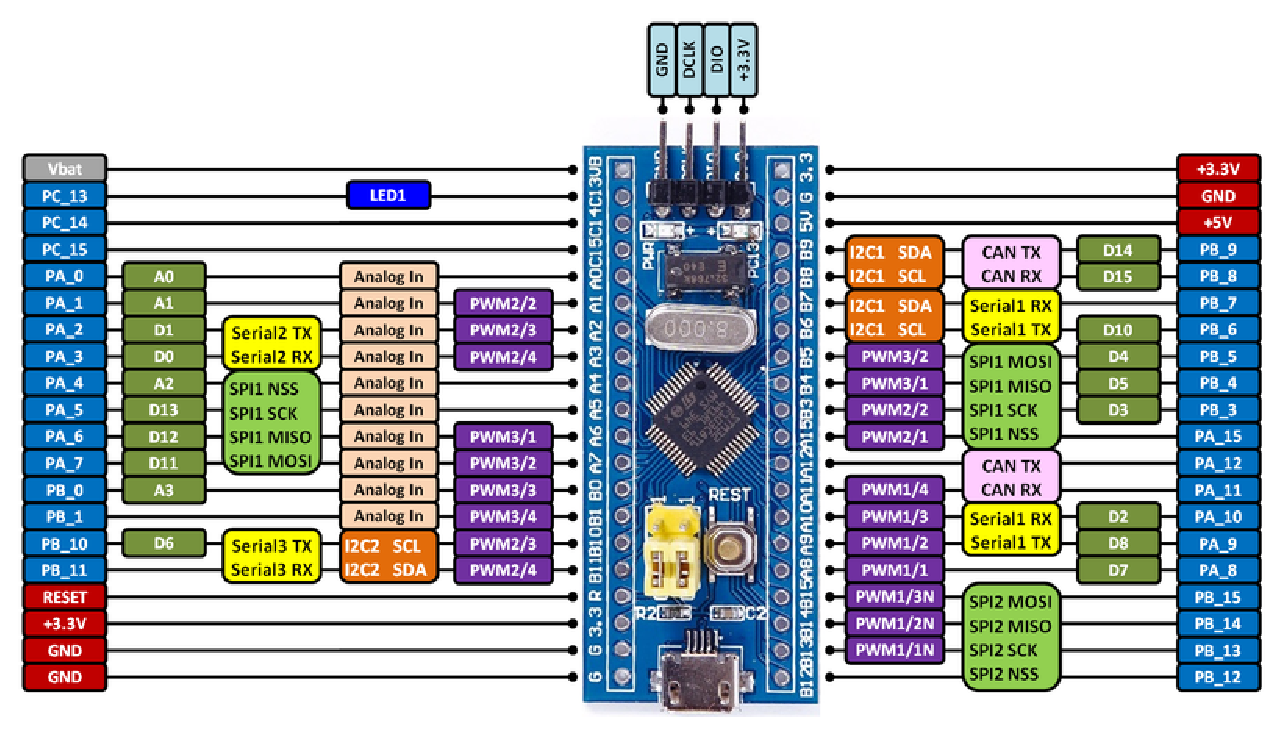
\includegraphics[width=\columnwidth]{./stm32/sevenseg/figs/stm_blue.eps}
\end{center}
\caption{Pin Connections of STM-32}
\label{fig:stm_blue}
\end{figure}
%
\begin{table}
\begin{center}
\input{./stm32/sevenseg/figs/stm_ssd}
\end{center}
\caption{STM-32 and Seven Segment Display Connections}
\label{table:stm_ssd}
\end{table}

\subsection{Software}
%
\item Before flashing code to STM32 set the STM32 board to Programming mode as shown in Fig. \ref{fig:programming_mode}, then change the mode to Operating mode as shown in Fig. \ref{fig:programming_mode} after flashing the code inorder to run your program from main memory.
\item Execute the following code 
\begin{lstlisting}
cd stm32/sevenseg/codes/sevenseg_example.c
\end{lstlisting}

%\begin{problem}
%	Connect the STM32 to the Raspberry Pi according to the \href{https://github.com/gadepall/EE4013/blob/master/setup/rpi/gvv_stm32_setup.pdf}{\url{instructions }} in
%\begin{lstlisting}
%https://github.com/gadepall/EE4013/blob/master/setup/rpi/gvv_stm32_setup.pdf
%\end{lstlisting}	
%\end{problem}
%\section{Display Control with STM32}
%
%\begin{problem}
%Follow the \href{https://github.com/gadepall/EE4013/blob/master/setup/tinker/gvv_stm32_tinker_setup.pdf}{\url{instructions }} in
%\begin{lstlisting}
%https://github.com/gadepall/EE4013/blob/master/setup/tinker/gvv_stm32_tinker_setup.pdf
%\end{lstlisting}
%to clone the \href{https://github.com/gadepall/EE4013/blob/master/setup/tinker/gvv_stm32_tinker_setup.pdf}{\url{repository }}
%\begin{lstlisting}[language=bash, frame=single, breaklines]
%https://github.com/gadepall/STM32F103C8T6
%\end{lstlisting}
%\end{problem}
%
%Fig. \ref{fig:sevenseg12} explains how to get decimal digits using the seven segment display. 
%\begin{problem}
%In the STM32F103C8T6 directory,
%\begin{lstlisting}
%cp sevenseg.c main.c
%\end{lstlisting}
%Generate the number 0 by executing \textbf{main.c} and flashing to the STM32. 
%\end{problem}	
%
%\begin{figure}[!h]
%\begin{center}
%\resizebox {0.8\columnwidth} {!} {
%\input{./figs/sevenseg12.tex}
%}
%\end{center}
%\caption{}
%\label{fig:sevenseg12}
%\end{figure}
%

\item Explain the process of generating the number 0 using the following instruction.
\begin{lstlisting}
GPIOB->ODR = 0xFC08;
\end{lstlisting}
\solution ODR is the Output Data Register, which is used to write outputs to the GPIO pins. The 16 bit number 0xFC08 on the RHS represents the pin configuration for the pins of port B of STM32F103C8T6, which are numbered PB15-PB0 in that order.  See Table \ref{table:stm_ssd}.
\\
\item Repeat the above exercise to generate the numbers 1-9 on the display.
\item The previous instructions set the bits in the unused ports PB15-PB10 and PB2-PB0. This may be undesirable in some cases. Generate 0 by not disturbing 
the unused pins.
\\
\solution The following instructions help accomplish this. The first instruction resets PB4-PB9.  The second instruction sets the PB3 pin. The other pins are
undisturbed.
\begin{lstlisting}
GPIOB->BRR = (1<<4)|(1<<5)|(1<<6)|(1<<7)|(1<<8)|(1<<9); // (Led ON)		
GPIOB->BSRR = (1<<3); // (Led OFF)					
\end{lstlisting}
%\section{Manual Display Control}
%\input{./chapters/chapter1}
%
\item Write a program to take a 4-bit BCD as input from hardware (GND or VDD) and show the next number on the seven segment display.
\\
\solution The following program takes 4 bits as input from pins PB12-PB15 and displays the output on a seven segment display. The next number
can be displayed by slightly modifying the code.
\begin{lstlisting}
cd codes/bin2dec_example.c
\end{lstlisting}
\end{enumerate}

\section{Dont Care}
\iffalse
\documentclass[journal,12pt,twocolumn]{IEEEtran}
%
\usepackage{setspace}
\usepackage{gensymb}
%\doublespacing
\singlespacing

%\usepackage{graphicx}
%\usepackage{amssymb}
%\usepackage{relsize}
\usepackage[cmex10]{amsmath}
\usepackage{siunitx}
%\usepackage{amsthm}
%\interdisplaylinepenalty=2500
%\savesymbol{iint}
%\usepackage{txfonts}
%\restoresymbol{TXF}{iint}
%\usepackage{wasysym}
\usepackage{amsthm}
%\usepackage{iithtlc}
\usepackage{mathrsfs}
\usepackage{txfonts}
\usepackage{stfloats}
\usepackage{steinmetz}
\usepackage{supertabular}
%\usepackage{bm}
\usepackage{cite}
\usepackage{cases}
\usepackage{subfig}
%\usepackage{xtab}
\usepackage{longtable}
\usepackage{multirow}
%\usepackage{algorithm}
%\usepackage{algpseudocode}
\usepackage{enumitem}
\usepackage{mathtools}
\usepackage{tikz}
\usepackage{circuitikz}
\usepackage{verbatim}
\usepackage{tfrupee}
\usepackage[breaklinks=true]{hyperref}
%\usepackage{stmaryrd}
\usepackage{tkz-euclide} % loads  TikZ and tkz-base
%\usetkzobj{all}
\usetikzlibrary{calc,math}
\usetikzlibrary{fadings}
\usepackage{listings}
    \usepackage{color}                                            %%
    \usepackage{array}                                            %%
    \usepackage{longtable}                                        %%
    \usepackage{calc}                                             %%
    \usepackage{multirow}                                         %%
    \usepackage{hhline}                                           %%
    \usepackage{ifthen}                                           %%
  %optionally (for landscape tables embedded in another document): %%
    \usepackage{lscape}     
\usepackage{multicol}
\usepackage{chngcntr}
\usepackage{blkarray}
\usepackage{karnaugh-map}
\usepackage{fontspec}
\usepackage[intoc]{nomencl}
\makenomenclature

%\usetikzlibrary{arrows, shapes.gates.logic.US, calc}
\usetikzlibrary{arrows,shapes.gates.logic.US,shapes.gates.logic.IEC,calc}
\setmainfont{Sanskrit_2003.ttf}
%\setmainfont{Nakula.ttf}
%\setmainfont{Lohit-Devanagari.ttf}


%\usepackage{enumerate}

%\usepackage{wasysym}
%\newcounter{MYtempeqncnt}
\DeclareMathOperator*{\Res}{Res}
%\renewcommand{\baselinestretch}{2}
\renewcommand\thesection{\arabic{section}}
\renewcommand\thesubsection{\thesection.\arabic{subsection}}
\renewcommand\thesubsubsection{\thesubsection.\arabic{subsubsection}}

\renewcommand\thesectiondis{\arabic{section}}
\renewcommand\thesubsectiondis{\thesectiondis.\arabic{subsection}}
\renewcommand\thesubsubsectiondis{\thesubsectiondis.\arabic{subsubsection}}

% correct bad hyphenation here
\hyphenation{op-tical net-works semi-conduc-tor}
\def\inputGnumericTable{}                                 %%


\lstset{
%language=shell,
%language = Prolog,
frame=single, 
breaklines=true,
%showstringspaces=false,
columns=fullflexible
literate = {-}{-}1
}
%\lstset{
%language=tex,
%frame=single, 
%breaklines=true
%}

\begin{document}
%


\newtheorem{theorem}{Theorem}[section]
\newtheorem{problem}{Problem}
\newtheorem{proposition}{Proposition}[section]
\newtheorem{lemma}{Lemma}[section]
\newtheorem{corollary}[theorem]{Corollary}
\newtheorem{example}{Example}[section]
\newtheorem{definition}[problem]{Definition}
%\newtheorem{thm}{Theorem}[section] 
%\newtheorem{defn}[thm]{Definition}
%\newtheorem{algorithm}{Algorithm}[section]
%\newtheorem{cor}{Corollary}
\newcommand{\BEQA}{\begin{eqnarray}}
\newcommand{\EEQA}{\end{eqnarray}}
\newcommand{\define}{\stackrel{\triangle}{=}}

\bibliographystyle{IEEEtran}
%\bibliographystyle{ieeetr}


\providecommand{\mbf}{\mathbf}
\providecommand{\pr}[1]{\ensuremath{\Pr\left(#1\right)}}
\providecommand{\qfunc}[1]{\ensuremath{Q\left(#1\right)}}
\providecommand{\sbrak}[1]{\ensuremath{{}\left[#1\right]}}
\providecommand{\lsbrak}[1]{\ensuremath{{}\left[#1\right.}}
\providecommand{\rsbrak}[1]{\ensuremath{{}\left.#1\right]}}
\providecommand{\brak}[1]{\ensuremath{\left(#1\right)}}
\providecommand{\lbrak}[1]{\ensuremath{\left(#1\right.}}
\providecommand{\rbrak}[1]{\ensuremath{\left.#1\right)}}
\providecommand{\cbrak}[1]{\ensuremath{\left\{#1\right\}}}
\providecommand{\lcbrak}[1]{\ensuremath{\left\{#1\right.}}
\providecommand{\rcbrak}[1]{\ensuremath{\left.#1\right\}}}
\providecommand{\ceil}[1]{\left \lceil #1 \right \rceil }
\theoremstyle{remark}
\newtheorem{rem}{Remark}
\newcommand{\sgn}{\mathop{\mathrm{sgn}}}
\providecommand{\abs}[1]{\left\vert#1\right\vert}
\providecommand{\res}[1]{\Res\displaylimits_{#1}} 
\providecommand{\norm}[1]{\left\lVert#1\right\rVert}
%\providecommand{\norm}[1]{\lVert#1\rVert}
\providecommand{\mtx}[1]{\mathbf{#1}}
\providecommand{\mean}[1]{E\left[ #1 \right]}
\providecommand{\fourier}{\overset{\mathcal{F}}{ \rightleftharpoons}}
%\providecommand{\hilbert}{\overset{\mathcal{H}}{ \rightleftharpoons}}
\providecommand{\system}{\overset{\mathcal{H}}{ \longleftrightarrow}}
	%\newcommand{\solution}[2]{\textbf{Solution:}{#1}}
\newcommand{\solution}{\noindent \textbf{Solution: }}
\newcommand{\cosec}{\,\text{cosec}\,}
\providecommand{\dec}[2]{\ensuremath{\overset{#1}{\underset{#2}{\gtrless}}}}
\newcommand{\myvec}[1]{\ensuremath{\begin{pmatrix}#1\end{pmatrix}}}
\newcommand{\mydet}[1]{\ensuremath{\begin{vmatrix}#1\end{vmatrix}}}
%\numberwithin{equation}{section}
\numberwithin{equation}{subsection}
%\numberwithin{problem}{section}
%\numberwithin{definition}{section}
\makeatletter
\@addtoreset{figure}{problem}
\makeatother

\let\StandardTheFigure\thefigure
\let\vec\mathbf
%\renewcommand{\thefigure}{\theproblem.\arabic{figure}}
%\renewcommand{\thefigure}{\theproblem}
\renewcommand{\thefigure}{\thesection}
%\setlist[enumerate,1]{before=\renewcommand\theequation{\theenumi.\arabic{equation}}
%\counterwithin{equation}{enumi}


%\renewcommand{\theequation}{\arabic{subsection}.\arabic{equation}}

\def\putbox#1#2#3{\makebox[0in][l]{\makebox[#1][l]{}\raisebox{\baselineskip}[0in][0in]{\raisebox{#2}[0in][0in]{#3}}}}
     \def\rightbox#1{\makebox[0in][r]{#1}}
     \def\centbox#1{\makebox[0in]{#1}}
     \def\topbox#1{\raisebox{-\baselineskip}[0in][0in]{#1}}
     \def\midbox#1{\raisebox{-0.5\baselineskip}[0in][0in]{#1}}

\vspace{3cm}

\title{
%	\logo{
Digital Design through Vaman
%	}
}
\author{ G. V. V. Sharma $^{*}$% <-this % stops a space
	\thanks{*The author is with the Department of Electrical Engineering, IIT Hyderabad, 502285, India. email: gadepall@ee.iith.ac.in.  All material in this document is released under GNU GPL.  Free to use for anything.}
	
}	
%\title{
%	\logo{Matrix Analysis through Octave}{\begin{center}\includegraphics[scale=.24]{tlc}\end{center}}{}{HAMDSP}
%}


% paper title
% can use linebreaks \\ within to get better formatting as desired
%\title{Matrix Analysis through Octave}
%
%
% author names and IEEE memberships
% note positions of commas and nonbreaking spaces ( ~ ) LaTeX will not break
% a structure at a ~ so this keeps an author's name from being broken across
% two lines.
% use \thanks{} to gain access to the first footnote area
% a separate \thanks must be used for each paragraph as LaTeX2e's \thanks
% was not built to handle multiple paragraphs
%

%\author{<-this % stops a space
%\thanks{}}
%}
% note the % following the last \IEEEmembership and also \thanks - 
% these prevent an unwanted space from occurring between the last author name
% and the end of the author line. i.e., if you had this:
% 
% \author{....lastname \thanks{...} \thanks{...} }
%                     ^------------^------------^----Do not want these spaces!
%
% a space would be appended to the last name and could cause every name on that
% line to be shifted left slightly. This is one of those "LaTeX things". For
% instance, "\textbf{A} \textbf{B}" will typeset as "A B" not "AB". To get
% "AB" then you have to do: "\textbf{A}\textbf{B}"
% \thanks is no different in this regard, so shield the last } of each \thanks
% that ends a line with a % and do not let a space in before the next \thanks.
% Spaces after \IEEEmembership other than the last one are OK (and needed) as
% you are supposed to have spaces between the names. For what it is worth,
% this is a minor point as most people would not even notice if the said evil
% space somehow managed to creep in.



% The paper headers
%\markboth{Journal of \LaTeX\ Class Files,~Vol.~6, No.~1, January~2007}%
%{Shell \MakeLowercase{\textit{et al.}}: Bare Demo of IEEEtran.cls for Journals}
% The only time the second header will appear is for the odd numbered pages
% after the title page when using the twoside option.
% 
% *** Note that you probably will NOT want to include the author's ***
% *** name in the headers of peer review papers.                   ***
% You can use \ifCLASSOPTIONpeerreview for conditional compilation here if
% you desire.




% If you want to put a publisher's ID mark on the page you can do it like
% this:
%\IEEEpubid{0000--0000/00\$00.00~\copyright~2007 IEEE}
% Remember, if you use this you must call \IEEEpubidadjcol in the second
% column for its text to clear the IEEEpubid mark.



% make the title area
\maketitle

\newpage

\tableofcontents


\bigskip

\renewcommand{\thefigure}{\theenumi}
\renewcommand{\thetable}{\theenumi}
%\renewcommand{\abstractname}{सार}
%\renewcommand{\nomname}{नामकरण}
%\renewcommand{\solution}{हल: }
%\renewcommand{\figurename}{आकृति.}
%\renewcommand{\tablename}{सारणी.}
%\renewcommand{\theequation}{\theenumi}

%\begin{abstract}
%%\boldmath
%In this letter, an algorithm for evaluating the exact analytical bit error rate  (BER)  for the piecewise linear (PL) combiner for  multiple relays is presented. Previous results were available only for upto three relays. The algorithm is unique in the sense that  the actual mathematical expressions, that are prohibitively large, need not be explicitly obtained. The diversity gain due to multiple relays is shown through plots of the analytical BER, well supported by simulations. 
%
%\end{abstract}
% IEEEtran.cls defaults to using nonbold math in the Abstract.
% This preserves the distinction between vectors and scalars. However,
% if the journal you are submitting to favors bold math in the abstract,
% then you can use LaTeX's standard command \boldmath at the very start
% of the abstract to achieve this. Many IEEE journals frown on math
% in the abstract anyway.

% Note that keywords are not normally used for peerreview papers.
%\begin{IEEEkeywords}
%Cooperative diversity, decode and forward, piecewise linear
%\end{IEEEkeywords}



% For peer review papers, you can put extra information on the cover
% page as needed:
% \ifCLASSOPTIONpeerreview
% \begin{center} \bfseries EDICS Category: 3-BBND \end{center}
% \fi
%
% For peerreview papers, this IEEEtran command inserts a page break and
% creates the second title. It will be ignored for other modes.
%\IEEEpeerreviewmaketitle
\fi

\begin{abstract}
The objective of this manual is to introduce beginners to arm embedded programming by powering a seven segment display.
\end{abstract}
\subsection{Components}
\renewcommand{\theequation}{\theenumi}
\renewcommand{\thefigure}{\theenumi}
\begin{enumerate}[label=\thesubsection.\arabic*.,ref=\thesubsection.\theenumi]
\numberwithin{equation}{enumi}
\numberwithin{figure}{enumi}
\numberwithin{table}{enumi}
\item The necessary components for this manual are listed in Table \ref{tabel:stm32/sevenseg/components}.
\begin{table}[!ht]
\begin{center}
\input{./stm32/sevenseg/figs/components.tex}
\end{center}
\caption{Components}
\label{tabel:stm32/sevenseg/components}
\end{table}
\subsection{Hardware}

%\subsection{Seven Segment Display}
%The breadboard can be divided into 5 segments.  In each of the green segements, the pins are internally connected so as to have the same voltage.  Similarly, in the central segments, the pins in each column  are internally connected in the same fashion as the blue columns. 

%\begin{problem}
%	Plug the display to the breadboard in Fig. \ref{fig:breadboard}
%\end{problem}
%\begin{figure}[!h]
%\begin{center}
%\includegraphics[width=\columnwidth]{./figs/breadboard}
%\end{center}
%\caption{}
%\label{fig:breadboard}
%\end{figure}
\item The seven segment display in Fig. \ref{fig:sevenseg} has eight pins, $a, b, c, d, e, f, g$ and $dot$ that take an active LOW input, i.e.  the LED will glow only if the input is connected to ground.  Each of these pins is connected to an LED segment.  The $dot$ pin is  reserved for the $\cdot$ LED.  

%
%\begin{center}
	%\includegraphics[scale=1]{sevenseg}
%\end{center}


\item Connect one end of the 1K resistor to the COM pin of the display and the other end to an extreme pin of the breadboard.	
%
%
%
%\begin{figure}[!h]
%\begin{center}
%\resizebox {0.5\columnwidth} {!} {
%\input{./figs/sevenseg.tex}
%}
%\end{center}
%\caption{}
%\label{fig:sevenseg}
%\end{figure}

\item The STM32F103C8T6 micro-controller in Fig. \ref{fig:stm_blue} has two ground pins, few analog input pins and few digital pins that can be used for both input as well as output. It has one Vcc (3.3V) pin that can generate 3.3$V$.  In the following exercises, only the GND, 3.3$V$ and digital pins will be used.
%
%
\item Make the pin connections in Table \ref{table:stm_ssd} using Figs. \ref{fig:sevenseg} and \ref{fig:stm_blue}.
	
%
\begin{figure}[!h]
\begin{center}
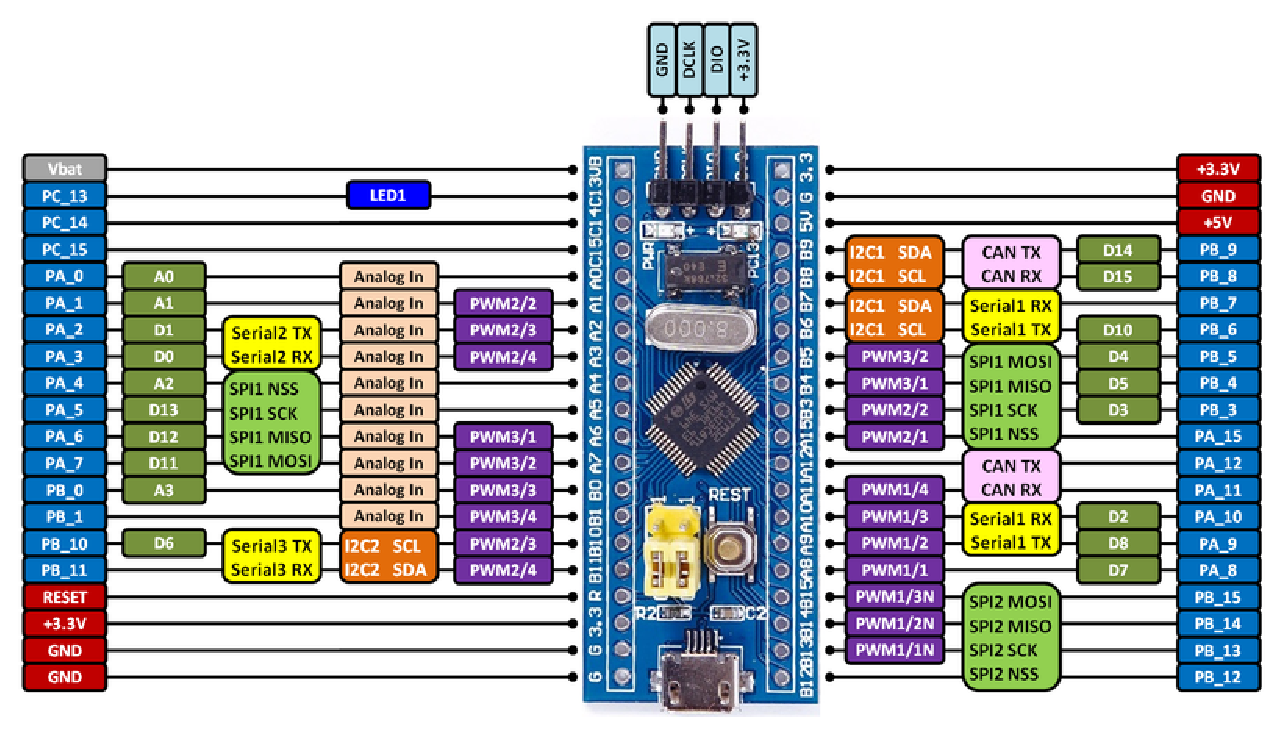
\includegraphics[width=\columnwidth]{./stm32/sevenseg/figs/stm_blue.eps}
\end{center}
\caption{Pin Connections of STM-32}
\label{fig:stm_blue}
\end{figure}
%
\begin{table}
\begin{center}
\input{./stm32/sevenseg/figs/stm_ssd}
\end{center}
\caption{STM-32 and Seven Segment Display Connections}
\label{table:stm_ssd}
\end{table}

\subsection{Software}
%
\item Before flashing code to STM32 set the STM32 board to Programming mode as shown in Fig. \ref{fig:programming_mode}, then change the mode to Operating mode as shown in Fig. \ref{fig:programming_mode} after flashing the code inorder to run your program from main memory.
\item Execute the following code 
\begin{lstlisting}
cd stm32/sevenseg/codes/sevenseg_example.c
\end{lstlisting}

%\begin{problem}
%	Connect the STM32 to the Raspberry Pi according to the \href{https://github.com/gadepall/EE4013/blob/master/setup/rpi/gvv_stm32_setup.pdf}{\url{instructions }} in
%\begin{lstlisting}
%https://github.com/gadepall/EE4013/blob/master/setup/rpi/gvv_stm32_setup.pdf
%\end{lstlisting}	
%\end{problem}
%\section{Display Control with STM32}
%
%\begin{problem}
%Follow the \href{https://github.com/gadepall/EE4013/blob/master/setup/tinker/gvv_stm32_tinker_setup.pdf}{\url{instructions }} in
%\begin{lstlisting}
%https://github.com/gadepall/EE4013/blob/master/setup/tinker/gvv_stm32_tinker_setup.pdf
%\end{lstlisting}
%to clone the \href{https://github.com/gadepall/EE4013/blob/master/setup/tinker/gvv_stm32_tinker_setup.pdf}{\url{repository }}
%\begin{lstlisting}[language=bash, frame=single, breaklines]
%https://github.com/gadepall/STM32F103C8T6
%\end{lstlisting}
%\end{problem}
%
%Fig. \ref{fig:sevenseg12} explains how to get decimal digits using the seven segment display. 
%\begin{problem}
%In the STM32F103C8T6 directory,
%\begin{lstlisting}
%cp sevenseg.c main.c
%\end{lstlisting}
%Generate the number 0 by executing \textbf{main.c} and flashing to the STM32. 
%\end{problem}	
%
%\begin{figure}[!h]
%\begin{center}
%\resizebox {0.8\columnwidth} {!} {
%\input{./figs/sevenseg12.tex}
%}
%\end{center}
%\caption{}
%\label{fig:sevenseg12}
%\end{figure}
%

\item Explain the process of generating the number 0 using the following instruction.
\begin{lstlisting}
GPIOB->ODR = 0xFC08;
\end{lstlisting}
\solution ODR is the Output Data Register, which is used to write outputs to the GPIO pins. The 16 bit number 0xFC08 on the RHS represents the pin configuration for the pins of port B of STM32F103C8T6, which are numbered PB15-PB0 in that order.  See Table \ref{table:stm_ssd}.
\\
\item Repeat the above exercise to generate the numbers 1-9 on the display.
\item The previous instructions set the bits in the unused ports PB15-PB10 and PB2-PB0. This may be undesirable in some cases. Generate 0 by not disturbing 
the unused pins.
\\
\solution The following instructions help accomplish this. The first instruction resets PB4-PB9.  The second instruction sets the PB3 pin. The other pins are
undisturbed.
\begin{lstlisting}
GPIOB->BRR = (1<<4)|(1<<5)|(1<<6)|(1<<7)|(1<<8)|(1<<9); // (Led ON)		
GPIOB->BSRR = (1<<3); // (Led OFF)					
\end{lstlisting}
%\section{Manual Display Control}
%\input{./chapters/chapter1}
%
\item Write a program to take a 4-bit BCD as input from hardware (GND or VDD) and show the next number on the seven segment display.
\\
\solution The following program takes 4 bits as input from pins PB12-PB15 and displays the output on a seven segment display. The next number
can be displayed by slightly modifying the code.
\begin{lstlisting}
cd codes/bin2dec_example.c
\end{lstlisting}
\end{enumerate}

\section{Problems}
\begin{enumerate}
	\item 		Obtain the Minimal Form for the Boolean Expression
\label{prob:2013/d/6/d}
\hfill (CBSE 2013)
		\begin{align}
\label{eq:2013/d/6/d}
H(P,Q,R,S)=\sum(0,1,2,3,5,7,8,9,10,14,15)
		\end{align}
	\item Write the POS form for the function G shown in Table
\ref{tab:2013/c/6/d}.
\label{prob:2013/c/6/d}
\hfill (CBSE 2013)

		\begin{table}[!ht]
			\centering
		\begin{tabular}{ |c |c |c |c |}
 \hline
 U  &  V  &  W  &  G\\
 \hline
 0  &  0  &  0  &  1\\
 \hline
 0  &  0  &  1  &  0\\
 \hline
 0  &  1  &  0  &  1\\
 \hline
 0  &  1  &  1  &  0\\
 \hline
 1  &  0  &  0  &  1\\
 \hline
 1  &  0  &  1  &  0\\
 \hline
 1  &  1  &  0  &  0\\
 \hline
 1  &  1  &  1  &  1\\
 \hline
 \end{tabular}
			\caption{}
\label{tab:2013/c/6/d}
 \end{table}
	\item Reduce the following Boolean Expression to its simplest form using K-Map 
\label{prob:2015-1/c/6/d}
\hfill (CBSE 2015)
		\begin{align}
\label{eq:2015-1/c/6/d}
			F(X,Y,Z,W)=(0,1,4,5,6,7,8,9,11,15)
		\end{align}
	\item 
		Derive a Canonical POS expression for a Boolean function F, represented by the following truth table 
\label{prob:2015-1/c/6/c}
\hfill (CBSE 2015)
		\begin{table}[!ht]
			\centering
		\begin{tabular}{|c|c|c|c|}
	\hline
X & Y & Z & F \\
\hline
0 & 0 & 0 & 1 \\  
\hline
0 & 0 & 1 & 0 \\ 
\hline
0 & 1 & 0 & 0 \\
\hline
0 & 1 & 1 & 1 \\
\hline
1 & 0 & 0 & 1 \\  
\hline
1 & 0 & 1 & 0 \\ 
\hline
1 & 1 & 0 & 0 \\
\hline
1 & 1 & 1 & 1 \\
\hline
\end{tabular}
		\caption{}
\label{tab:2015-1/c/6/c}
\end{table}
	\item 
\label{prob:2015/c/6/d}
\hfill (CBSE 2015)
		Reduce the following Boolean Expression to its simplest form using K-map
		\begin{align}
\label{eq:2015/c/6/d}
F(X,Y,Z,W)= \sum (0,1,6,8,9,10,11,12,15)
		\end{align}
	\item Reduce the following Boolean Expression to its simplest form using K-map.
\label{prob:2016/c/6/d}
\hfill (CBSE 2016)
		\begin{align}
\label{eq:2016/c/6/d}
			F(X,Y,Z,W)= \sum(2,6,7,8,9,10,11,13,14,15)
		\end{align}
	\item Derive a Canonical POS expression for a Boolean function  F, represented in Table
\ref{tab:2016/c/6/c}
\hfill (CBSE 2016)
\label{prob:2016/c/6/c}
		\begin{table}[!ht]
			\centering
			\begin{tabular}{|c|c|c|c|}
	\iffalse
	{0.8\textwidth} { 
  | >{\centering\arraybackslash}X 
  | >{\centering\arraybackslash}X 
  | >{\centering\arraybackslash}X | 
  | >{\centering\arraybackslash}X |
  }
  \fi
 \hline
 P & Q & R & F(P,  Q,  R) \\
 \hline
 0  & 0  & 0 & 0  \\
\hline
0  & 0  & 1 & 1  \\
\hline
0  & 1  & 0 & 1  \\
\hline
0  & 1  & 1 & 0  \\
\hline
1  & 0  & 0 & 0  \\
\hline
1  & 0  & 1 & 0  \\
\hline
1  & 1  & 0 & 1  \\
\hline
1  & 1  & 1 & 1  \\
\hline
\end{tabular}
			\caption{}
\label{tab:2016/c/6/c}
		\end{table}
	\item Verify the following 
\hfill (CBSE 2016)
\label{prob:2016/c/6/a}
		\begin{align}
\label{eq:2016/c/6/a}
A'+B'C = A'B'C' + A'BC' + A'BC + A'B'C + AB'C
		\end{align}


	\item Reduce the following boolean expression to it's simplest form using K-Map
\hfill (CBSE 2017)
\label{prob:2017-1/c/6/d}
		\begin{align}
F(X,Y,Z,W) = \sum(0,1,2,3,4,5,10,11,14)
\label{eq:2017-1/c/6/d}
		\end{align}
	\item
		Reduce the following Boolean Expression to its simplest form using K-Map.
\hfill (CBSE 2017)
\label{prob:2017/c/6/d}
		\begin{align}
E(U,V,Z,W)=   (2 , 3 , 6 , 8 , 9 , 10 , 11 , 12 , 13 )
\label{eq:2017/c/6/d}
		\end{align}
	\item Derive a canonical POS expression for a Boolean function $G$, represented by Table 
\ref{tab:2017/c/6/c}
\label{prob:2017/c/6/c}
\hfill (CBSE 2017)
		\begin{table}[htbp]
 \begin{center}
    \begin{tabular}{|l|c|c|c|c|c|c|c|c|} \hline 
  \textbf{X}& \textbf{Y} & \textbf{Z} &\textbf{G(X,Y,Z)} \\
 \hline
 0&0&0&0\\ \hline
0&0&1&0 \\ \hline
0&1&0&1\\ \hline
0&1&1&0  \\ \hline
1&0&0&1\\ \hline
1&0&1&1\\ \hline
1&1&0&0\\ \hline
1&1&1&1\\ \hline
\end{tabular}   
\end{center}
\caption{}
\label{tab:2017/c/6/c}
\end{table}
\item Derive a canonical POS expression for a Boolean function $FN$, represented by Table 
\ref{tab:2018/c/6/c}.
\label{prob:2018/c/6/c}
\hfill (CBSE 2018)
		\begin{table}[!ht]
			\centering
\begin{tabular}{|l|c|r|l|c|}
    \hline % <-- Alignments: 1st column left, 2nd middle and 3rd right, with vertical lines in between
      \textbf{X} & \textbf{Y} & \textbf{Z} & \textbf{FN(X,Y,Z)}\\
      \hline
      0 & 0 & 0 & 1\\
\hline
      0 & 0 & 1 & 1\\
\hline
      0 & 1 & 0 & 0\\
\hline
      0 & 1 & 1 & 0\\
\hline
      1 & 0 & 0 & 1\\
\hline
      1 & 0 & 1 & 0\\
\hline
      1 & 1 & 0 & 0\\
\hline
      1 & 1 & 1 & 1\\
      \hline      
   \end{tabular}
\caption{}
\label{tab:2018/c/6/c}
   \end{table}

\item 
	Reduce the following Boolean expression in the simplest form using K-Map.
		\begin{align}
F(P,Q,R,S) = \sum (0,1,2,3,5,6,7,10,14,15)
		\end{align}
\hfill (CBSE 2019)
\label{prob:2019/c/6/d}
%
\item Fig. \ref{fig:2020/gate/ec/10} below shows a muliplexer where S0 and S1 are the select lines, I0 to I3 are the input lines, EN is the enable line and F(P,Q,R) is the output. Find the boolean expression for output F as function of inputs P,Q,R using K-map. 
%
\label{prob:2020/gate/ec/10}
\hfill (GATE EC 2020)
\begin{figure}[ht]
\centering
	\includegraphics[width=1\columnwidth]{figs/2020-gate-ec-10.png}
\caption{}
\label{fig:2020/gate/ec/10}
\end{figure}
%
\item
	The four variable function $f$ is given in terms of min-terms as
		\begin{align}
	    f(A,B,C,D) = \sum m(2,3,8,10,11,12,14,15)
\label{eq:1991/gate/ec/9}
		\end{align}
	    Using the K-map minimize the function in the sum of products form. 
\label{prob:1991/gate/ec/9}
\hfill (GATE EC 1991)
\item Find the logic realized by the circuit in Fig. 
\ref{fig:1992/gate/ec/1/22}.
\label{prob:1992/gate/ec/1/22}
\hfill (GATE EC 1992)
\begin{figure}[ht]
\centering
	\includegraphics[width=1\columnwidth]{figs/1992-gate-ec-1-22.png}
\caption{}
\label{fig:1992/gate/ec/1/22}
\end{figure}
\item
	A combinational circuit has three inputs A, B and C and an output F. F is true only for the following input combinations. 
\hfill (GATE EC 1992)
\label{prob:1992/gate/ec/2/9}
	\begin{enumerate}
		\item A is false and B is true 
		\item A is false and C is true 
		\item A, B and C are all false 
		\item A, B and C are all true 
	\end{enumerate}
	\begin{enumerate}
\item Write the truth table for F. use the convention, true = 1 and false = 0. 
\item Write the simplified expression for F as a Sum of Products. 
\item Write the simplified expression for F as a product of Sums.
\end{enumerate}
\item Draw the logic circuit for Table 
\ref{tab:1993/gate/ec/5/7} using only NOR gates.
\label{prob:1993/gate/ec/5/7}
\hfill (GATE EC 1993)
	\begin{table}[!ht]
		\centering
		\begin{tabular}{|c|c|c|c|}
\hline
\textbf{C} &\textbf{B} & \textbf{A} & \textbf{Y} \\
\hline
0 & 0 & 0 & 1 \\  
\hline
0 & 0 & 1 & 1 \\ 
\hline
0 & 1 & 0 & 1 \\
\hline
0 & 1 & 1 & 0 \\
\hline
1 & 0 & 0 & 1 \\  
\hline
1 & 0 & 1 & 0 \\ 
\hline
1 & 1 & 0 & 0 \\
\hline
1 & 1 & 1& 0\\
\hline
\end{tabular}
\caption{}
\label{tab:1993/gate/ec/5/7}
\end{table}
\item
	Implement the following Boolean function in a 8x1 multiplexer.
\label{prob:1993/gate/ec/14}
\hfill (GATE EC 1993)
		\begin{align}
\label{eq:1993/gate/ec/14}
 Q = BC + ABD' + A'C'D  
		\end{align}
	\item Minimize the following Boolean function in 
\ref{eq:1999/gate/ec/2/10}.
\label{prob:1999/gate/ec/2/10}
		\begin{equation}
\label{eq:1999/gate/ec/2/10}
F= A'B'C'+A'BC'+A'BC+ABC'
\end{equation}
%
\item Find the Boolean expression for Table
\ref{tab:2005-gate-ec-54}.
\label{prob:2005-gate-ec-54}
\hfill (GATE EC 2005)
	\begin{table}[htbp]
		\centering
    \begin{tabular}{|l|c|c|c|c|c|c|c|c} \hline \textbf{A}
  & \textbf{B} & \textbf{C} & \textbf{X} \\
 \hline
        0&0&0&0 \\
        \hline
        0&0&1&0 \\
        \hline
        0&1&0&0 \\
        \hline
        0&1&1&1 \\
        \hline
        1&0&0&0 \\
        \hline
        1&0&1&0 \\
        \hline
        1&1&0&1 \\
        \hline
        1&1&1&0  \\
        \hline
\end{tabular}   
\caption{}
\label{tab:2005-gate-ec-54}
\end{table}
\item Minimize the logic function represented by the following Karnaugh map.
\label{prob:2010-gate-ee-52}
\hfill (CBSE 2021)
	\begin{karnaugh-map}[4][2][1][$YZ$][$X$]
		\manualterms{1,1,0,1,0,0,0,1}
	%	\implicant{0}{1}
	%	\implicant{3}{7}
	\end{karnaugh-map}	
\item Find the output for the Karnaugh map shown below
\label{tab:2019-gate-ec-34}
\hfill (GATE EE 2019)
	\begin{karnaugh-map}[4][4][1][$PQ$][$RS$]

		\minterms{1,3,4,5,7,6,12,13,15,14}
		\maxterms{0,2,8,9,10,11}

%		\implicant{4}{14}
%		\implicant{1}{7}
	\end{karnaugh-map}
\item The propogation delays of the XOR gate, AND gate and multiplexer (MUX) in the circuit shown in the Fig.
\ref{fig:2021-gate-ec-31}
	are 4 ns, 2 ns and 1 ns, respectively.
\label{prob:2021-gate-ec-31}
If all the inputs P, Q, R, S and T are applied simultaneously and held constant, the maximum propogation delay of the circuit is
\hfill (Gate EC-2021)
\begin{enumerate}
	\item 3 ns \item 5 ns \item 6 ns \item 7 ns
\end{enumerate}
\begin{figure}[!htb]
	\centering
\begin{tikzpicture}                                   
\ctikzset{                                            logic ports=ieee,                                     logic ports/scale=0.8                                 }                                            
\node[and port] (a) at (1,6){};                       
\node[xor port] (b) at (1,4){};                       
\node[and port] (c) at (1,2){};                       
\node[and port] (e) at (7,3){};                       
\draw(-1,6.23) node[above]{$P$} -- (0.25,6.23);       
\draw(-1,5.23) node[above]{$Q$} -- (0.17,5.23);       
\draw(-1,2.95) node[above]{$R$} -- (0.17,2.95);       
\draw(-1,1.77) node[above]{$S$} -- (0.25,1.77);       
\draw(a.in 2) -| (b.in 1);                            
\draw(b.in 2) -| (c.in 1);                            
\draw(b.out) -- ++(1.4,0) node{0};                   
\draw(c.out) -- ++(1.4,0) node{1};                    
\draw(e.out) -- ++(0.4,0) node{1};                    
\draw(a.out) -- ++(6.4,0) node{0};                    
\draw(6.15,3.25) -- (6.15,6);                         
\draw(4.95,2.78) -- (6.15,2.78);                              
\draw(0,0) node[above]{$T$} -- (10,0);                
\draw(10,0) -- (10,0.5) node[above]{$S0$};           
\draw(4,0) -- (4,1.25) node[above]{$S0$};             
\draw(11.87,4.5) -- (14,4.5) node[above]{$Y$};                                                            
\tikzstyle{mux} = [rectangle, draw, minimum     height = 10em, text width = 5em]                      
\node[mux] (d) at (4,3) {MUX};                                
\tikzstyle{mux}=[rectangle,draw,minimum height=20em,text width=10em]                                      
\node[mux] (f) at (10,4){MUX};
\end{tikzpicture}

	\caption{}
\label{fig:2021-gate-ec-31}
\end{figure}
\item 
\label{prob:2012-gate-ec-19}
Consider the 2-bit multiplexer(MUX) shown in the figure. For output to be the XOR of R and S, the values for $ W,X,Y$ and $Z$ are ? 
\hfill (GATE EC-2022)
\begin{figure}[h]

\begin{circuitikz}

\draw (7,2)coordinate (E) -- (9,2)coordinate (F) -- (9,-1)coordinate (G) -- (7,-1)coordinate (H) -- (7,2)coordinate (E);
\draw (11,2)coordinate (I) -- (13,2)coordinate (J) -- (13,-1)coordinate (K) -- (11,-1)coordinate (L) -- (11,2)coordinate (I);
% AND Gate
\draw (6,1.5) node[and port] (and) {};
\draw (and.in 1) node[left] {};
\draw (and.in 2) node[left] {};
\draw (and.out) |- ($(E)!0.2!(H)$)--++(0:0)node[right]{$D1$}; % and gate output is connected to d1.

%clock
\draw ($(L)!0.5!(K)$)node[anchor=south]{$clk$};
\draw ($(H)!0.5!(G)$)node[anchor=south]{$clk$};
\draw(6,-2) node[above]{$12 \textsl{KHz}$} |- (12,-2);
\draw ($(H)!0.5!(G)$)node[anchor=south,xshift=6]{}--++(90:-1)--++(0:0)node[left]{};
\draw ($(L)!0.5!(K)$)node[anchor=south,xshift=6]{}--++(90:-1)--++(0:0)node[left]{};

\draw($(F)!0.2!(G)$)node[left]{$Q1$} -- ($(I)!0.2!(L)$)node[right]{$D2$}; % q1 is connected to d2.
    
\draw($(F)!0.8!(G)$)node[left]{$\overline{Q1}$};
    
\draw($(J)!0.2!(K)$)node[left]{$Q2$};
    
\draw($(J)!0.8!(K)$)node[left]{$\overline{Q2}$};
    
    
\draw ($(J)!0.2!(K)$)--++(0:1)node[right]{};
    
\draw(and.in 1) --++(90:2)-|(9.5,1)|-($(F)!0.8!(G)$)(0:0)node[left]{}; % and gate input 1 is connected to q1 bar.
    
\draw(and.in 2) --++(-90:4)-|(13.5,-0.5)|- ($(J)!0.8!(K)$);  % and gate input 2 is connected to q2 bar.
    
\end{circuitikz}

\caption{}
\label{fig:2012-gate-ec-19}
\end{figure}
\begin{enumerate}
\item $W = 0, X = 0, Y = 1, Z = 1$
\item $W = 1, X = 0, Y = 1, Z = 0$
\item $W = 0, X = 1, Y = 1, Z = 0$
\item $W = 1, X = 1, Y = 0, Z = 0$
\end{enumerate}
\end{enumerate}

\chapter{7474}
\iffalse
\documentclass[journal,12pt,twocolumn]{IEEEtran}
%
\usepackage{setspace}
\usepackage{gensymb}
%\doublespacing
\singlespacing

%\usepackage{graphicx}
%\usepackage{amssymb}
%\usepackage{relsize}
\usepackage[cmex10]{amsmath}
\usepackage{siunitx}
%\usepackage{amsthm}
%\interdisplaylinepenalty=2500
%\savesymbol{iint}
%\usepackage{txfonts}
%\restoresymbol{TXF}{iint}
%\usepackage{wasysym}
\usepackage{amsthm}
%\usepackage{iithtlc}
\usepackage{mathrsfs}
\usepackage{txfonts}
\usepackage{stfloats}
\usepackage{steinmetz}
\usepackage{supertabular}
%\usepackage{bm}
\usepackage{cite}
\usepackage{cases}
\usepackage{subfig}
%\usepackage{xtab}
\usepackage{longtable}
\usepackage{multirow}
%\usepackage{algorithm}
%\usepackage{algpseudocode}
\usepackage{enumitem}
\usepackage{mathtools}
\usepackage{tikz}
\usepackage{circuitikz}
\usepackage{verbatim}
\usepackage{tfrupee}
\usepackage[breaklinks=true]{hyperref}
%\usepackage{stmaryrd}
\usepackage{tkz-euclide} % loads  TikZ and tkz-base
%\usetkzobj{all}
\usetikzlibrary{calc,math}
\usetikzlibrary{fadings}
\usepackage{listings}
    \usepackage{color}                                            %%
    \usepackage{array}                                            %%
    \usepackage{longtable}                                        %%
    \usepackage{calc}                                             %%
    \usepackage{multirow}                                         %%
    \usepackage{hhline}                                           %%
    \usepackage{ifthen}                                           %%
  %optionally (for landscape tables embedded in another document): %%
    \usepackage{lscape}     
\usepackage{multicol}
\usepackage{chngcntr}
\usepackage{blkarray}
\usepackage{karnaugh-map}
\usepackage{fontspec}
\usepackage[intoc]{nomencl}
\makenomenclature

%\usetikzlibrary{arrows, shapes.gates.logic.US, calc}
\usetikzlibrary{arrows,shapes.gates.logic.US,shapes.gates.logic.IEC,calc}
\setmainfont{Sanskrit_2003.ttf}
%\setmainfont{Nakula.ttf}
%\setmainfont{Lohit-Devanagari.ttf}


%\usepackage{enumerate}

%\usepackage{wasysym}
%\newcounter{MYtempeqncnt}
\DeclareMathOperator*{\Res}{Res}
%\renewcommand{\baselinestretch}{2}
\renewcommand\thesection{\arabic{section}}
\renewcommand\thesubsection{\thesection.\arabic{subsection}}
\renewcommand\thesubsubsection{\thesubsection.\arabic{subsubsection}}

\renewcommand\thesectiondis{\arabic{section}}
\renewcommand\thesubsectiondis{\thesectiondis.\arabic{subsection}}
\renewcommand\thesubsubsectiondis{\thesubsectiondis.\arabic{subsubsection}}

% correct bad hyphenation here
\hyphenation{op-tical net-works semi-conduc-tor}
\def\inputGnumericTable{}                                 %%


\lstset{
%language=shell,
%language = Prolog,
frame=single, 
breaklines=true,
%showstringspaces=false,
columns=fullflexible
literate = {-}{-}1
}
%\lstset{
%language=tex,
%frame=single, 
%breaklines=true
%}

\begin{document}
%


\newtheorem{theorem}{Theorem}[section]
\newtheorem{problem}{Problem}
\newtheorem{proposition}{Proposition}[section]
\newtheorem{lemma}{Lemma}[section]
\newtheorem{corollary}[theorem]{Corollary}
\newtheorem{example}{Example}[section]
\newtheorem{definition}[problem]{Definition}
%\newtheorem{thm}{Theorem}[section] 
%\newtheorem{defn}[thm]{Definition}
%\newtheorem{algorithm}{Algorithm}[section]
%\newtheorem{cor}{Corollary}
\newcommand{\BEQA}{\begin{eqnarray}}
\newcommand{\EEQA}{\end{eqnarray}}
\newcommand{\define}{\stackrel{\triangle}{=}}

\bibliographystyle{IEEEtran}
%\bibliographystyle{ieeetr}


\providecommand{\mbf}{\mathbf}
\providecommand{\pr}[1]{\ensuremath{\Pr\left(#1\right)}}
\providecommand{\qfunc}[1]{\ensuremath{Q\left(#1\right)}}
\providecommand{\sbrak}[1]{\ensuremath{{}\left[#1\right]}}
\providecommand{\lsbrak}[1]{\ensuremath{{}\left[#1\right.}}
\providecommand{\rsbrak}[1]{\ensuremath{{}\left.#1\right]}}
\providecommand{\brak}[1]{\ensuremath{\left(#1\right)}}
\providecommand{\lbrak}[1]{\ensuremath{\left(#1\right.}}
\providecommand{\rbrak}[1]{\ensuremath{\left.#1\right)}}
\providecommand{\cbrak}[1]{\ensuremath{\left\{#1\right\}}}
\providecommand{\lcbrak}[1]{\ensuremath{\left\{#1\right.}}
\providecommand{\rcbrak}[1]{\ensuremath{\left.#1\right\}}}
\providecommand{\ceil}[1]{\left \lceil #1 \right \rceil }
\theoremstyle{remark}
\newtheorem{rem}{Remark}
\newcommand{\sgn}{\mathop{\mathrm{sgn}}}
\providecommand{\abs}[1]{\left\vert#1\right\vert}
\providecommand{\res}[1]{\Res\displaylimits_{#1}} 
\providecommand{\norm}[1]{\left\lVert#1\right\rVert}
%\providecommand{\norm}[1]{\lVert#1\rVert}
\providecommand{\mtx}[1]{\mathbf{#1}}
\providecommand{\mean}[1]{E\left[ #1 \right]}
\providecommand{\fourier}{\overset{\mathcal{F}}{ \rightleftharpoons}}
%\providecommand{\hilbert}{\overset{\mathcal{H}}{ \rightleftharpoons}}
\providecommand{\system}{\overset{\mathcal{H}}{ \longleftrightarrow}}
	%\newcommand{\solution}[2]{\textbf{Solution:}{#1}}
\newcommand{\solution}{\noindent \textbf{Solution: }}
\newcommand{\cosec}{\,\text{cosec}\,}
\providecommand{\dec}[2]{\ensuremath{\overset{#1}{\underset{#2}{\gtrless}}}}
\newcommand{\myvec}[1]{\ensuremath{\begin{pmatrix}#1\end{pmatrix}}}
\newcommand{\mydet}[1]{\ensuremath{\begin{vmatrix}#1\end{vmatrix}}}
%\numberwithin{equation}{section}
\numberwithin{equation}{subsection}
%\numberwithin{problem}{section}
%\numberwithin{definition}{section}
\makeatletter
\@addtoreset{figure}{problem}
\makeatother

\let\StandardTheFigure\thefigure
\let\vec\mathbf
%\renewcommand{\thefigure}{\theproblem.\arabic{figure}}
%\renewcommand{\thefigure}{\theproblem}
\renewcommand{\thefigure}{\thesection}
%\setlist[enumerate,1]{before=\renewcommand\theequation{\theenumi.\arabic{equation}}
%\counterwithin{equation}{enumi}


%\renewcommand{\theequation}{\arabic{subsection}.\arabic{equation}}

\def\putbox#1#2#3{\makebox[0in][l]{\makebox[#1][l]{}\raisebox{\baselineskip}[0in][0in]{\raisebox{#2}[0in][0in]{#3}}}}
     \def\rightbox#1{\makebox[0in][r]{#1}}
     \def\centbox#1{\makebox[0in]{#1}}
     \def\topbox#1{\raisebox{-\baselineskip}[0in][0in]{#1}}
     \def\midbox#1{\raisebox{-0.5\baselineskip}[0in][0in]{#1}}

\vspace{3cm}

\title{
%	\logo{
Digital Design through Vaman
%	}
}
\author{ G. V. V. Sharma $^{*}$% <-this % stops a space
	\thanks{*The author is with the Department of Electrical Engineering, IIT Hyderabad, 502285, India. email: gadepall@ee.iith.ac.in.  All material in this document is released under GNU GPL.  Free to use for anything.}
	
}	
%\title{
%	\logo{Matrix Analysis through Octave}{\begin{center}\includegraphics[scale=.24]{tlc}\end{center}}{}{HAMDSP}
%}


% paper title
% can use linebreaks \\ within to get better formatting as desired
%\title{Matrix Analysis through Octave}
%
%
% author names and IEEE memberships
% note positions of commas and nonbreaking spaces ( ~ ) LaTeX will not break
% a structure at a ~ so this keeps an author's name from being broken across
% two lines.
% use \thanks{} to gain access to the first footnote area
% a separate \thanks must be used for each paragraph as LaTeX2e's \thanks
% was not built to handle multiple paragraphs
%

%\author{<-this % stops a space
%\thanks{}}
%}
% note the % following the last \IEEEmembership and also \thanks - 
% these prevent an unwanted space from occurring between the last author name
% and the end of the author line. i.e., if you had this:
% 
% \author{....lastname \thanks{...} \thanks{...} }
%                     ^------------^------------^----Do not want these spaces!
%
% a space would be appended to the last name and could cause every name on that
% line to be shifted left slightly. This is one of those "LaTeX things". For
% instance, "\textbf{A} \textbf{B}" will typeset as "A B" not "AB". To get
% "AB" then you have to do: "\textbf{A}\textbf{B}"
% \thanks is no different in this regard, so shield the last } of each \thanks
% that ends a line with a % and do not let a space in before the next \thanks.
% Spaces after \IEEEmembership other than the last one are OK (and needed) as
% you are supposed to have spaces between the names. For what it is worth,
% this is a minor point as most people would not even notice if the said evil
% space somehow managed to creep in.



% The paper headers
%\markboth{Journal of \LaTeX\ Class Files,~Vol.~6, No.~1, January~2007}%
%{Shell \MakeLowercase{\textit{et al.}}: Bare Demo of IEEEtran.cls for Journals}
% The only time the second header will appear is for the odd numbered pages
% after the title page when using the twoside option.
% 
% *** Note that you probably will NOT want to include the author's ***
% *** name in the headers of peer review papers.                   ***
% You can use \ifCLASSOPTIONpeerreview for conditional compilation here if
% you desire.




% If you want to put a publisher's ID mark on the page you can do it like
% this:
%\IEEEpubid{0000--0000/00\$00.00~\copyright~2007 IEEE}
% Remember, if you use this you must call \IEEEpubidadjcol in the second
% column for its text to clear the IEEEpubid mark.



% make the title area
\maketitle

\newpage

\tableofcontents


\bigskip

\renewcommand{\thefigure}{\theenumi}
\renewcommand{\thetable}{\theenumi}
%\renewcommand{\abstractname}{सार}
%\renewcommand{\nomname}{नामकरण}
%\renewcommand{\solution}{हल: }
%\renewcommand{\figurename}{आकृति.}
%\renewcommand{\tablename}{सारणी.}
%\renewcommand{\theequation}{\theenumi}

%\begin{abstract}
%%\boldmath
%In this letter, an algorithm for evaluating the exact analytical bit error rate  (BER)  for the piecewise linear (PL) combiner for  multiple relays is presented. Previous results were available only for upto three relays. The algorithm is unique in the sense that  the actual mathematical expressions, that are prohibitively large, need not be explicitly obtained. The diversity gain due to multiple relays is shown through plots of the analytical BER, well supported by simulations. 
%
%\end{abstract}
% IEEEtran.cls defaults to using nonbold math in the Abstract.
% This preserves the distinction between vectors and scalars. However,
% if the journal you are submitting to favors bold math in the abstract,
% then you can use LaTeX's standard command \boldmath at the very start
% of the abstract to achieve this. Many IEEE journals frown on math
% in the abstract anyway.

% Note that keywords are not normally used for peerreview papers.
%\begin{IEEEkeywords}
%Cooperative diversity, decode and forward, piecewise linear
%\end{IEEEkeywords}



% For peer review papers, you can put extra information on the cover
% page as needed:
% \ifCLASSOPTIONpeerreview
% \begin{center} \bfseries EDICS Category: 3-BBND \end{center}
% \fi
%
% For peerreview papers, this IEEEtran command inserts a page break and
% creates the second title. It will be ignored for other modes.
%\IEEEpeerreviewmaketitle
\fi

\begin{abstract}
The objective of this manual is to introduce beginners to arm embedded programming by powering a seven segment display.
\end{abstract}
\subsection{Components}
\renewcommand{\theequation}{\theenumi}
\renewcommand{\thefigure}{\theenumi}
\begin{enumerate}[label=\thesubsection.\arabic*.,ref=\thesubsection.\theenumi]
\numberwithin{equation}{enumi}
\numberwithin{figure}{enumi}
\numberwithin{table}{enumi}
\item The necessary components for this manual are listed in Table \ref{tabel:stm32/sevenseg/components}.
\begin{table}[!ht]
\begin{center}
\input{./stm32/sevenseg/figs/components.tex}
\end{center}
\caption{Components}
\label{tabel:stm32/sevenseg/components}
\end{table}
\subsection{Hardware}

%\subsection{Seven Segment Display}
%The breadboard can be divided into 5 segments.  In each of the green segements, the pins are internally connected so as to have the same voltage.  Similarly, in the central segments, the pins in each column  are internally connected in the same fashion as the blue columns. 

%\begin{problem}
%	Plug the display to the breadboard in Fig. \ref{fig:breadboard}
%\end{problem}
%\begin{figure}[!h]
%\begin{center}
%\includegraphics[width=\columnwidth]{./figs/breadboard}
%\end{center}
%\caption{}
%\label{fig:breadboard}
%\end{figure}
\item The seven segment display in Fig. \ref{fig:sevenseg} has eight pins, $a, b, c, d, e, f, g$ and $dot$ that take an active LOW input, i.e.  the LED will glow only if the input is connected to ground.  Each of these pins is connected to an LED segment.  The $dot$ pin is  reserved for the $\cdot$ LED.  

%
%\begin{center}
	%\includegraphics[scale=1]{sevenseg}
%\end{center}


\item Connect one end of the 1K resistor to the COM pin of the display and the other end to an extreme pin of the breadboard.	
%
%
%
%\begin{figure}[!h]
%\begin{center}
%\resizebox {0.5\columnwidth} {!} {
%\input{./figs/sevenseg.tex}
%}
%\end{center}
%\caption{}
%\label{fig:sevenseg}
%\end{figure}

\item The STM32F103C8T6 micro-controller in Fig. \ref{fig:stm_blue} has two ground pins, few analog input pins and few digital pins that can be used for both input as well as output. It has one Vcc (3.3V) pin that can generate 3.3$V$.  In the following exercises, only the GND, 3.3$V$ and digital pins will be used.
%
%
\item Make the pin connections in Table \ref{table:stm_ssd} using Figs. \ref{fig:sevenseg} and \ref{fig:stm_blue}.
	
%
\begin{figure}[!h]
\begin{center}
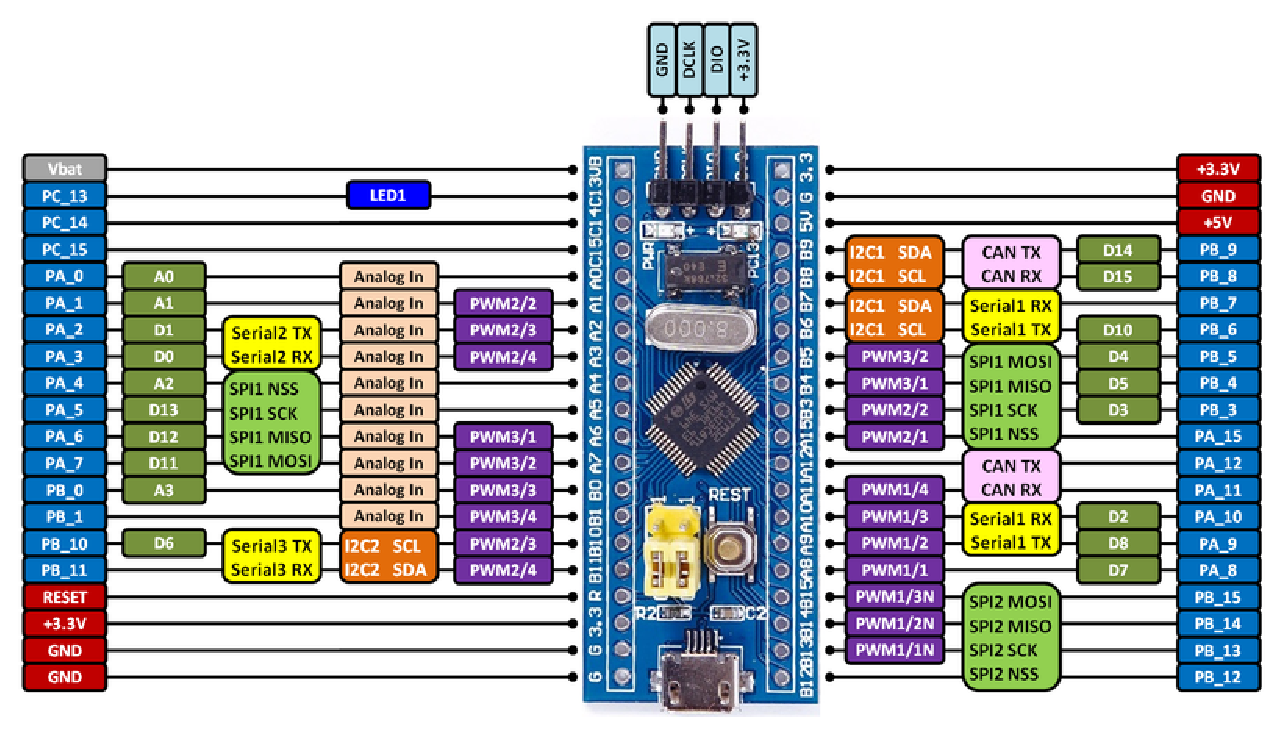
\includegraphics[width=\columnwidth]{./stm32/sevenseg/figs/stm_blue.eps}
\end{center}
\caption{Pin Connections of STM-32}
\label{fig:stm_blue}
\end{figure}
%
\begin{table}
\begin{center}
\input{./stm32/sevenseg/figs/stm_ssd}
\end{center}
\caption{STM-32 and Seven Segment Display Connections}
\label{table:stm_ssd}
\end{table}

\subsection{Software}
%
\item Before flashing code to STM32 set the STM32 board to Programming mode as shown in Fig. \ref{fig:programming_mode}, then change the mode to Operating mode as shown in Fig. \ref{fig:programming_mode} after flashing the code inorder to run your program from main memory.
\item Execute the following code 
\begin{lstlisting}
cd stm32/sevenseg/codes/sevenseg_example.c
\end{lstlisting}

%\begin{problem}
%	Connect the STM32 to the Raspberry Pi according to the \href{https://github.com/gadepall/EE4013/blob/master/setup/rpi/gvv_stm32_setup.pdf}{\url{instructions }} in
%\begin{lstlisting}
%https://github.com/gadepall/EE4013/blob/master/setup/rpi/gvv_stm32_setup.pdf
%\end{lstlisting}	
%\end{problem}
%\section{Display Control with STM32}
%
%\begin{problem}
%Follow the \href{https://github.com/gadepall/EE4013/blob/master/setup/tinker/gvv_stm32_tinker_setup.pdf}{\url{instructions }} in
%\begin{lstlisting}
%https://github.com/gadepall/EE4013/blob/master/setup/tinker/gvv_stm32_tinker_setup.pdf
%\end{lstlisting}
%to clone the \href{https://github.com/gadepall/EE4013/blob/master/setup/tinker/gvv_stm32_tinker_setup.pdf}{\url{repository }}
%\begin{lstlisting}[language=bash, frame=single, breaklines]
%https://github.com/gadepall/STM32F103C8T6
%\end{lstlisting}
%\end{problem}
%
%Fig. \ref{fig:sevenseg12} explains how to get decimal digits using the seven segment display. 
%\begin{problem}
%In the STM32F103C8T6 directory,
%\begin{lstlisting}
%cp sevenseg.c main.c
%\end{lstlisting}
%Generate the number 0 by executing \textbf{main.c} and flashing to the STM32. 
%\end{problem}	
%
%\begin{figure}[!h]
%\begin{center}
%\resizebox {0.8\columnwidth} {!} {
%\input{./figs/sevenseg12.tex}
%}
%\end{center}
%\caption{}
%\label{fig:sevenseg12}
%\end{figure}
%

\item Explain the process of generating the number 0 using the following instruction.
\begin{lstlisting}
GPIOB->ODR = 0xFC08;
\end{lstlisting}
\solution ODR is the Output Data Register, which is used to write outputs to the GPIO pins. The 16 bit number 0xFC08 on the RHS represents the pin configuration for the pins of port B of STM32F103C8T6, which are numbered PB15-PB0 in that order.  See Table \ref{table:stm_ssd}.
\\
\item Repeat the above exercise to generate the numbers 1-9 on the display.
\item The previous instructions set the bits in the unused ports PB15-PB10 and PB2-PB0. This may be undesirable in some cases. Generate 0 by not disturbing 
the unused pins.
\\
\solution The following instructions help accomplish this. The first instruction resets PB4-PB9.  The second instruction sets the PB3 pin. The other pins are
undisturbed.
\begin{lstlisting}
GPIOB->BRR = (1<<4)|(1<<5)|(1<<6)|(1<<7)|(1<<8)|(1<<9); // (Led ON)		
GPIOB->BSRR = (1<<3); // (Led OFF)					
\end{lstlisting}
%\section{Manual Display Control}
%\input{./chapters/chapter1}
%
\item Write a program to take a 4-bit BCD as input from hardware (GND or VDD) and show the next number on the seven segment display.
\\
\solution The following program takes 4 bits as input from pins PB12-PB15 and displays the output on a seven segment display. The next number
can be displayed by slightly modifying the code.
\begin{lstlisting}
cd codes/bin2dec_example.c
\end{lstlisting}
\end{enumerate}

\chapter{Finite State Machine}
\iffalse
\documentclass[journal,2pt,twocolumn]{IEEEtran}
%
\usepackage{setspace}
\usepackage{gensymb}
\usepackage{xcolor}
\usepackage{caption}
\usepackage[hyphens,spaces,obeyspaces]{url}
%\usepackage{subcaption}
%\doublespacing
\singlespacing

%\usepackage{graphicx}
%\usepackage{amssymb}
%\usepackage{relsize}
\usepackage[cmex0]{amsmath}
\usepackage{mathtools}
%\usepackage{amsthm}
%\interdisplaylinepenalty=2500
%\savesymbol{iint}
%\usepackage{txfonts}
%\restoresymbol{TXF}{iint}
%\usepackage{wasysym}
\usepackage{amsthm}
\usepackage{mathrsfs}
\usepackage{txfonts}
\usepackage{stfloats}
\usepackage{cite}
\usepackage{cases}
\usepackage{subfig}
%\usepackage{xtab}
\usepackage{longtable}
\usepackage{multirow}
%\usepackage{algorithm}
%\usepackage{algpseudocode}
\usepackage{enumerate}
\usepackage{mathtools}
\usepackage{eenrc}
%\usepackage[framemethod=tikz]{mdframed}
\usepackage[breaklinks]{hyperref}
%\usepackage{breakcites}
\usepackage{listings}
    \usepackage[latin]{inputenc}                                 %%
    \usepackage{color}                                            %%
    \usepackage{array}                                            %%
    \usepackage{longtable}                                        %%
    \usepackage{calc}                                             %%
    \usepackage{multirow}                                         %%
    \usepackage{hhline}                                           %%
    \usepackage{ifthen}                                           %%
  %optionally (for landscape tables embedded in another document): %%
    \usepackage{lscape}     

\usepackage{tikz}
\usepackage{circuitikz}
\usepackage{karnaugh-map}
\usepackage{pgf}
\usepackage[hyphenbreaks]{breakurl}

%\usepackage{url}
%\def\UrlBreaks{\do\/\do-}





%\usepackage{stmaryrd}


%\usepackage{wasysym}
%\newcounter{MYtempeqncnt}
\DeclareMathOperator*{\Res}{Res}
%\renewcommand{\baselinestretch}{2}
\renewcommand\thesection{\arabic{section}}
\renewcommand\thesubsection{\thesection\arabic{subsection}}
\renewcommand\thesubsubsection{\thesubsection\arabic{subsubsection}}

\renewcommand\thesectiondis{\arabic{section}}
\renewcommand\thesubsectiondis{\thesectiondis\arabic{subsection}}
\renewcommand\thesubsubsectiondis{\thesubsectiondis\arabic{subsubsection}}

% correct bad hyphenation here
\hyphenation{op-tical net-works semi-conduc-tor}

%\lstset{
%language=C,
%frame=single, 
%breaklines=true
%}

%\lstset{
	%%basicstyle=\small\ttfamily\bfseries,
	%%numberstyle=\small\ttfamily,
	%language=Octave,
	%backgroundcolor=\color{white},
	%%frame=single,
	%%keywordstyle=\bfseries,
	%%breaklines=true,
	%%showstringspaces=false,
	%%xleftmargin=-0mm,
	%%aboveskip=-mm,
	%%belowskip=0mm
%}

%\surroundwithmdframed[width=\columnwidth]{lstlisting}
\def\inputGnumericTable{}                                 %%
\lstset{
%language=C,
frame=single, 
breaklines=true,
columns=fullflexible
}
 

\begin{document}
%

\theoremstyle{definition}
\newtheorem{theorem}{Theorem}[section]
\newtheorem{problem}{Problem}
\newtheorem{proposition}{Proposition}[section]
\newtheorem{lemma}{Lemma}[section]
\newtheorem{corollary}[theorem]{Corollary}
\newtheorem{example}{Example}[section]
\newtheorem{definition}{Definition}[section]
%\newtheorem{algorithm}{Algorithm}[section]
%\newtheorem{cor}{Corollary}
\newcommand{\BEQA}{\begin{eqnarray}}
\newcommand{\EEQA}{\end{eqnarray}}
\newcommand{\define}{\stackrel{\triangle}{=}}

\bibliographystyle{IEEEtran}
%\bibliographystyle{ieeetr}

\providecommand{\nCr}[2]{\,^{#}C_{#2}} % nCr
\providecommand{\nPr}[2]{\,^{#}P_{#2}} % nPr
\providecommand{\mbf}{\mathbf}
\providecommand{\pr}{\ensuremath{\Pr\left(#\right)}}
\providecommand{\qfunc}{\ensuremath{Q\left(#\right)}}
\providecommand{\sbrak}{\ensuremath{{}\left[#\right]}}
\providecommand{\lsbrak}{\ensuremath{{}\left[#\right}}
\providecommand{\rsbrak}{\ensuremath{{}\left#\right]}}
\providecommand{\brak}{\ensuremath{\left(#\right)}}
\providecommand{\lbrak}{\ensuremath{\left(#\right}}
\providecommand{\rbrak}{\ensuremath{\left#\right)}}
\providecommand{\cbrak}{\ensuremath{\left\{#\right\}}}
\providecommand{\lcbrak}{\ensuremath{\left\{#\right}}
\providecommand{\rcbrak}{\ensuremath{\left#\right\}}}
\providecommand{\ceil}{\left \lceil # \right \rceil }
\theoremstyle{remark}
\newtheorem{rem}{Remark}
\newcommand{\sgn}{\mathop{\mathrm{sgn}}}
\providecommand{\abs}{\left\vert#\right\vert}
\providecommand{\res}{\Res\displaylimits_{#}} 
\providecommand{\norm}{\lVert#\rVert}
\providecommand{\mtx}{\mathbf{#}}
\providecommand{\mean}{E\left[ # \right]}
\providecommand{\fourier}{\overset{\mathcal{F}}{ \rightleftharpoons}}
%\providecommand{\hilbert}{\overset{\mathcal{H}}{ \rightleftharpoons}}
\providecommand{\system}{\overset{\mathcal{H}}{ \longleftrightarrow}}
	%\newcommand{\solution}[2]{\textbf{Solution:}{#}}
\newcommand{\solution}{\noindent \textbf{Solution: }}
\providecommand{\dec}[2]{\ensuremath{\overset{#}{\underset{#2}{\gtrless}}}}
%\numberwithin{equation}{subsection}
\numberwithin{equation}{section}
%\numberwithin{problem}{subsection}
%\numberwithin{definition}{subsection}
\makeatletter
\@addtoreset{figure}{problem}
\makeatother

\let\StandardTheFigure\thefigure
%\renewcommand{\thefigure}{\theproblem\arabic{figure}}
\renewcommand{\thefigure}{\theproblem}


%\numberwithin{figure}{subsection}

%\numberwithin{equation}{subsection}
%\numberwithin{equation}{section}
%%\numberwithin{equation}{problem}
%%\numberwithin{problem}{subsection}
\numberwithin{problem}{section}
%%\numberwithin{definition}{subsection}
%\makeatletter
%\@addtoreset{figure}{problem}
%\makeatother
\makeatletter
\@addtoreset{table}{problem}
\makeatother

\let\StandardTheFigure\thefigure
\let\StandardTheTable\thetable
%%\renewcommand{\thefigure}{\theproblem\arabic{figure}}
%\renewcommand{\thefigure}{\theproblem}
\renewcommand{\thetable}{\theproblem}
%%\numberwithin{figure}{section}

%%\numberwithin{figure}{subsection}

\vspace{3cm}

\title{ 
	\logo{
Finite State Machine
	}
}



% paper title
% can use linebreaks \\ within to get better formatting as desired
%\title{Matrix Analysis through Octave}
%
%
% author names and IEEE memberships
% note positions of commas and nonbreaking spaces ( ~ ) LaTeX will not break
% a structure at a ~ so this keeps an author's name from being broken across
% two lines
% use \thanks{} to gain access to the first footnote area
% a separate \thanks must be used for each paragraph as LaTeX2e's \thanks
% was not built to handle multiple paragraphs
%

\author{G V V Sharma$^{*}$% <-this % stops a space
\thanks{*The author is with the Department
of Electrical Engineering, Indian Institute of Technology, Hyderabad
502285 India e-mail:  gadepall@iithacin All content in this manual is released under GNU GPL  Free and open source}% <-this % stops a space
%\thanks{J Doe and J Doe are with Anonymous University}% <-this % stops a space
%\thanks{Manuscript received April 9, 2005; revised January , 2007}}
}
% note the % following the last \IEEEmembership and also \thanks - 
% these prevent an unwanted space from occurring between the last author name
% and the end of the author line ie, if you had this:
% 
% \author{lastname \thanks{} \thanks{} }
%                     ^------------^------------^----Do not want these spaces!
%
% a space would be appended to the last name and could cause every name on that
% line to be shifted left slightly This is one of those "LaTeX things" For
% instance, "\textbf{A} \textbf{B}" will typeset as "A B" not "AB" To get
% "AB" then you have to do: "\textbf{A}\textbf{B}"
% \thanks is no different in this regard, so shield the last } of each \thanks
% that ends a line with a % and do not let a space in before the next \thanks
% Spaces after \IEEEmembership other than the last one are OK (and needed) as
% you are supposed to have spaces between the names For what it is worth,
% this is a minor point as most people would not even notice if the said evil
% space somehow managed to creep in



% The paper headers
%\markboth{Journal of \LaTeX\ Class Files,~Vol~6, No~, January~2007}%
%{Shell \MakeLowercase{\textit{et al}}: Bare Demo of IEEEtrancls for Journals}
% The only time the second header will appear is for the odd numbered pages
% after the title page when using the twoside option
% 
% *** Note that you probably will NOT want to include the author's ***
% *** name in the headers of peer review papers                   ***
% You can use \ifCLASSOPTIONpeerreview for conditional compilation here if
% you desire




% If you want to put a publisher's ID mark on the page you can do it like
% this:
%\IEEEpubid{0000--0000/00\$0000~\copyright~2007 IEEE}
% Remember, if you use this you must call \IEEEpubidadjcol in the second
% column for its text to clear the IEEEpubid mark



% make the title area
\maketitle

\tableofcontents

\bigskip

\renewcommand{\thefigure}{\theenumi}
\renewcommand{\thetable}{\theenumi}


\begin{abstract}
%\boldmath
	\fi
We explain  a state machine by deconstructing the decade counter

\section{The Decade Counter}
The block diagram of a decade counter (repeatedly counts up from 0 to 9)
is available in Fig \ref{fig:decade_counter}  The {\em incrementing } decoder
and {\em display} decoder are part of {\em combinational} logic, while
the {\em delay} is part of {\em sequential} logic
\iffalse
\begin{figure}[!h]
\resizebox {\columnwidth} {!} {
\input{ide/fsm/figs/decade_counter}
}
\caption{The decade counter}
\label{fig:decade_counter}
\end{figure}
\fi
%
\section{Finite State Machine}
%
\begin{enumerate}

\item Fig \ref{fig:fsm_counter} shows a {\em finite state machine} (FSM) diagram for the decade counter in Fig \ref{fig:decade_counter}  $s_0$ is the state when the input to the incrementing decoder is 0  The {\em state transition table} for the FSM is Table \ref{tab:ide/7447/counter_decoder},
%	0 in \cite{gvv_kmap}
		where the present state is denoted by the variables $W,X,Y,Z$ and the next state by $A,B,C,D$.  
\begin{figure}[!h]
\centering
%\resizebox {\columnwidth} {!} {
\input{ide/fsm/figs/fsm_counter}
%}
\caption{FSM for the decade counter}
\label{fig:fsm_counter}
\end{figure}
\item The FSM implementation is available in Fig \ref{fig:dff}  The {\em flip-flops} hold the input for the time that is given by the {\em clock}  This is nothing but the implementation of the {\em Delay} block in Fig \ref{fig:decade_counter}
%
\begin{figure}[!h]
\resizebox {\columnwidth} {!} {
\input{ide/fsm/figs/dff}
}
\caption{Decade counter FSM implementation using D-Flip Flops}
\label{fig:dff}
\end{figure}
%
\item The hardware cost of the system is given by
\begin{equation}
\text{No of D Flip-Flops} = \myceil{\log_{2}\brak{\text{No of States}}}
\end{equation}
For the FSM in Fig \ref{fig:fsm_counter}, the number of states is 9, hence the number flipflops required = 4  
\item Draw the state transition diagram for 
a decade down counter (counts from 9 to 0 repeatedly) using an FSM  
\item Write the state transition table for the down counter
\item Obtain the state transition equations with and without don't cares
\item Verify your design using an arduino
%\item Repeat the above exercises by designing a circuit that can detect 3 consecutive s in a bitstream 
\end{enumerate}



\section{Problems}
\begin{enumerate}
	\item The digital circuit shown in Fig. \ref{fig:2004-gate-ee-68} generates a modified clockpulse at the output. Sketch the output waveform.
\label{prob:2004-gate-ee-68}
\hfill (GATE EE 2004)


\begin{figure}[h]
	\centering
	\includegraphics[width=\columnwidth]{figs/2004-gate-ee-68.jpg}
	\caption{}
\label{fig:2004-gate-ee-68}
\end{figure}
\item The circuit shown in the figure below uses ideal positive edge-triggered synchronous J-K flip flops with outputs X and Y. If the initial state of the output is X=0 and Y=0, just before the arrival of the first clock pulse, the state of the output just before the arrival of the second clock pulse is
\label{prob:2019-gate-in-12}
\hfill (GATE IN 2019)
\begin{figure}[!h]
	\begin{center} 
	    \includegraphics[width=\columnwidth]{figs/2019-gate-in-12.png}
	\end{center}
\caption{}
\label{fig:2019-gate-in-12}
\end{figure}
\item 	The state diagram of a sequence detector is shown in
  \figref{fig:gate/ec/2020/39/1}		
		. State $S_0$ is the initial state of the sequence detector. If the output is 1, then
\hfill (GATE EC 2020)
 \begin{figure}[h]
	 \centering
  \begin{tikzpicture}                                   
\ctikzset{                                            logic ports=ieee,                                     logic ports/scale=0.8                                 }                                            
\node[and port] (a) at (1,6){};                       
\node[xor port] (b) at (1,4){};                       
\node[and port] (c) at (1,2){};                       
\node[and port] (e) at (7,3){};                       
\draw(-1,6.23) node[above]{$P$} -- (0.25,6.23);       
\draw(-1,5.23) node[above]{$Q$} -- (0.17,5.23);       
\draw(-1,2.95) node[above]{$R$} -- (0.17,2.95);       
\draw(-1,1.77) node[above]{$S$} -- (0.25,1.77);       
\draw(a.in 2) -| (b.in 1);                            
\draw(b.in 2) -| (c.in 1);                            
\draw(b.out) -- ++(1.4,0) node{0};                   
\draw(c.out) -- ++(1.4,0) node{1};                    
\draw(e.out) -- ++(0.4,0) node{1};                    
\draw(a.out) -- ++(6.4,0) node{0};                    
\draw(6.15,3.25) -- (6.15,6);                         
\draw(4.95,2.78) -- (6.15,2.78);                              
\draw(0,0) node[above]{$T$} -- (10,0);                
\draw(10,0) -- (10,0.5) node[above]{$S0$};           
\draw(4,0) -- (4,1.25) node[above]{$S0$};             
\draw(11.87,4.5) -- (14,4.5) node[above]{$Y$};                                                            
\tikzstyle{mux} = [rectangle, draw, minimum     height = 10em, text width = 5em]                      
\node[mux] (d) at (4,3) {MUX};                                
\tikzstyle{mux}=[rectangle,draw,minimum height=20em,text width=10em]                                      
\node[mux] (f) at (10,4){MUX};
\end{tikzpicture}

  \caption{State diagram}
  \label{fig:gate/ec/2020/39/1}		
  \end{figure}	 
\begin{enumerate}
 \item the sequence 01010 is detected
 \item the sequence 01011 is detected
 \item the sequence 01110 is detected
 \item the sequence 01001 is detected	 
\end{enumerate}	
	\item 		
		A counter is constructed with three D flip-flops. The input-output pairs are named (D0, Q0), (D1, Q1), and (D2, Q2), where the subscript 0 denotes the least significant bit. The output sequence is desired to be the Gray-code sequence 000, 001, 011, 010, 110, 111, 101, and 100, repeating periodically. Note that the bits are listed in the Q2 Q1 Q0 format. Find the combinational logic expression for D1.
\label{prob:2021-gate-ee-37}
\hfill (GATE EE 2021)
\iffalse
\item The propogation delay of the exclusive-OR(XOR) gate in the circuit in Fig.
\label{prob:2021-gate-ec-46}
\ref{fig:2021-gate-ec-46}
is 3ns. The propogation delay of all the flip-flops is assumed to be zero. The clock(Clk) frequency provided to the circuit is 500MHz.
\begin{figure}[!h]
\begin{center}
\resizebox{0.5\columnwidth}{!}{
\begin{tikzpicture}
\ctikzset{                                   
logic ports=ieee,                   
logic ports/scale=0.5               
}                                    
\draw(-1.3,0)node[xor port,anchor=out](x) {};         
\tikzstyle{dff}=[rectangle,draw,minimum height=7em,text width=7em,inner sep=3em]                                       
\node[dff] (dff2) {D2};                             
\node[dff, right=2cm of dff2] (dff1) {D1};           
\node[dff, right=2cm of dff1] (dff0) {D0};        
%Connecting flip-flops together                    
\draw (dff2.out) -- ++(2,0) node[above]{};        
\draw (dff1.out) -- ++(2,0) node[above] {};         
\draw (dff0.out) -- ++(2,0) node[above]{};          
\draw(dff2.out) -| (2.3,1.5) node[above]{$Q2$};        
\draw(dff1.out) -|(6.8,1.2) node[above]{$Q1$};         
\draw(dff0.out) -|(12.4,2) node[above]{$Q0$};          
\draw(x.in 2) -|(-3,2)to[short] (12.4,2);              
\draw(x.in 1)-|(-2.5,1.5)to[short](2.3,1.5);          
\draw(-2,-2) node[above]{$Clk$} --(6,-2);            
\draw(6,-2) node[above]{} --(9.1,-2);                 
\draw(9.1,-2)--(9.1,-1.2) node[above]{};                 
\draw(8.9,-1.23)--(9.1,-1)--(9.3,-1.23);               
\draw(4.5,-2)--(4.5,-1.2) node[above]{};               
\draw(4.3,-1.23)--(4.5,-1)--(4.7,-1.23);            
\draw(0,-2)--(0,-1.2) node[above]{};               
\draw(-0.2,-1.23)--(0,-1)--(0.2,-1.23);
\end{tikzpicture}

}
\end{center}
	\caption{Circuit}
\label{fig:2021-gate-ec-46}
\end{figure}
%
Starting from the initial value of the flip-flop outputs $Q2Q1Q0 =111$ with $D2=1$,the minimum number of triggering clock edges after which the flip-flop outputs $Q2Q1Q0$ becomes 1 0 0\emph{(in integer)} is \line(1,0){12.5}
\hfill (GATE EC 2021)
\fi
\item 
\label{prob:2022-gate-ec-43}
	 For the circuit shown in Fig. 
\ref{fig:2022-gate-ec-43},
		the clock frequency is $f_0$ and the duty cycle is $25 \%$. For the signal at the $Q$ output of the Flip-Flop,
\begin{enumerate}
	\item frequency of $\frac{f_0}{4}$ and duty cycle is 50$\%$
	\item frequency of $\frac{f_0}{4}$ and duty cycle is 25$\%$
	\item frequency of $\frac{f_0}{2}$ and duty cycle is 50$\%$
	\item frequency of $f_0$ and duty cycle is 25$\%$ \\
\end{enumerate}
\begin{figure}[h]
	\centering
\begin{tikzpicture}
    \draw (2,2) rectangle (5,5);
    \draw (3.5,5) node[above]{$2$ $Bit$ $binary$ $counter$};
    \draw (3.3,2) -- (3.5,2.2) -- (3.7,2);
    \draw (7,2) rectangle (10,5);
    \draw (8.5,5) node[above]{$Flip-Flop$};
    \draw (8.3,2) -- (8.5,2.2) -- (8.7,2);
    \draw (5,3) -- (5.5,3) node[above]{$MSB$} -- (6,3);
    \draw (7.25,3) node{$K$};
    \draw (5,4) -- (5.5,4) node[above]{$LSB$} -- (7,4);
    \draw (7.25,4) node{$J$};
    \draw (6.75,4) -- (6.75,3) -- (7,3);
    \draw (0,0) node[above]{$clock$} -- (8.5,0);
    \draw (3.5,0) -- (3.5,2);
    \draw (8.5,0) -- (8.5,2);
    \draw (10,3) -- (11,3);
    \draw (9.75,4) node{$Q$} (10,4) -- (11,4);
\end{tikzpicture}

	\caption{}
\label{fig:2022-gate-ec-43}
\end{figure}
\hfill 	(GATE EC-2022)

\item A sequence detector is designed to detect precisely 3 digital inputs, with overlapping sequences detectable. For the sequence $(1,0,1)$ and input data $(1,1,0,1,0,0,1,1,0,1,0,1,1,0)$, what is the output of this detector?
		\begin{enumerate}
			\item 1,1,0,0,0,0,1,1,0,1,0,0
			\item 0,1,0,0,0,0,0,1,0,1,0,0
			\item 0,1,0,0,0,0,0,1,0,1,1,0
			\item 0,1,0,0,0,0,0,0,1,0,0,0
		\end{enumerate}
		\hfill (GATE EE 2020)
\item 
 Two T-flip flops are interconnected as shown in \figref{fig:tff1}. The present state of the flip flops are: $A = 1, B = 1$. The input x is given as $1, 0, 1$ in the next three clock cycles. The decimal equivalent of $(ABy)_{2}$ with A being the MSB and y being the LSB, after the 3\textsuperscript{rd} clock cycle is \rule{12mm}{0.4pt}

		\vspace{1cm}
	\begin{figure}[ht]
		\centering
		\begin{tikzpicture}
  \draw (0,0) rectangle (2,3);

  \draw (-4,2.25) -- (0,2.25);
  \draw (-0.5,0.75) -- (0,0.75);
  \node[left] at (0.75,2.25) {$T_B$};
  \node[left] at (1.1,0.75) {$clk$};

  \draw (2,2.25) -- (4,2.25);
  \node[left] at (2,2.25) {$B$};
  

  \draw (0,0.4) -- (0.4,0.75) -- (0,1.1);

  \draw (0,4) rectangle (2,7);
  
  \draw (-0.5,6.25) -- (0,6.25);
  \draw (-0.5,4.75) -- (0,4.75);
  \node[left] at (0.75,6.25) {$T_A$};
  \node[left] at (1.1,4.75) {$clk$};

  \draw (-1.5,6.25) node[nand port] (nand) {};
  \draw (-4.5,6.525) -- (nand.in 1);
  \node[left] at (-4.5,6.525) {$x$};
  \draw (-2.9,3.5) -- (nand.in 2) ;
  \draw (nand.out) -- (-0.5,6.25) ;
  \draw (-4,2.25) -- (-4,6.525) ;
  \draw (-2.9,3.5) -- (3.5,3.5) ;
  \draw (3.5,3.5) -- (3.5,2.25) ;
  \filldraw (3.5,2.25) circle (2pt) ;
  \filldraw (-4,6.525) circle (2pt) ;
  \filldraw (-0.5,0.75) circle (2pt);

  \draw (5.5,5.965) node[or port] (or) {};
  \draw (4,6.25) -- (or.in 1) ;
  \draw (4,2.25) -- (4,5.685) ;
  \draw (4,5.685) -- (or.in 2) ;
  \node[right] at (or.out) {$y$} ;
  \draw (-0.5,4.75) -- (-0.5,-1.) ;
  \node[below] at (-0.5,-1.) {$clk$};
  
  \draw (2,6.25) -- (4,6.25);
  \node[left] at (2,6.25) {$A$};

  \draw (0,4.4) -- (0.4,4.75) -- (0,5.1);
  
\end{tikzpicture}
		\caption{}
		\label{fig:tff1}
		\hfill (GATE IN 2020)
	\end{figure}


\item In the circuit shown below,\ref{fig:image} a positive edge-triggered D flip-flop is used for sampling input data
 using clock CK.The XOR gate outputs 3.3 volts for logic HIGH and 0 volts for logic LOW levels.
The data bit and clock periods are equal and the value of $ \Delta T / T_{ck} $ = 0.15,where
the parameters $ \Delta T $ and $ T_ck$ are shown in the figure.Assume  that the Flip and
the XOR gate are ideal.  
\begin{figure}[!ht] 
    \includegraphics[scale=0.4]{figs/image.png} 
    \caption{image}
    \label{fig:image}
 \end{figure}
\label{fig:2018-gate-ec-46}
\hfill(GATE EC 2018)
\item A 2-bit synchronous counter using two J-K flip flops is shown. The expressions for the inputs to the J-K flip flops are also shown in the figure. The output sequence of the counter starting from $Q_1Q_2 = 00$ is 
\begin{figure}[!ht]
	\centering
	\includegraphics[width=\columnwidth]{figs/question44.png}
	\caption{$2$-bit synchronous counter}
	\label{fig:enter-label}
\end{figure}
\begin{enumerate}
	\item $00\rightarrow11\rightarrow10\rightarrow01\rightarrow00...$ 
        \item $00\rightarrow01\rightarrow10\rightarrow11\rightarrow00...$
        \item $00\rightarrow01\rightarrow11\rightarrow10\rightarrow00...$
        \item $00\rightarrow10\rightarrow11\rightarrow01\rightarrow00...$
\end{enumerate}
\hfill{GATE IN 2018}
        \item Let $p$ and $q$ be two propositions. Consider the following two formulae in propositional logic.
			\begin{align}
				 S_1 : ( \rightharpoondown p \vee (p \wedge q))\rightarrow q \\
				 S_2 : q\rightarrow(\rightharpoondown p \vee (p \wedge q))
			\end{align}
        Which one of the following choices is correct?
		                                          \hfill(GATE-CS2021)
		\begin{enumerate}[label=(\Alph*)]
			\item Both $S_1$ and $S_2$ are tautologies.
			\item $S_1$ is a tautology but $S_2$ is not a tautology.
			\item $S_1$ is not a tautology but $S_2$ is a tautology.
			\item Neither $S_1$ nor $S_2$ is a tautology.
		\end{enumerate}
\item Consider a $3$-bit counter, designed using T flip-flops, as shown below:
     \begin{figure}[H]
\centering
\includegraphics[width=\columnwidth]{ide/fsm/figs/3bitcounter.jpg}
\caption{}
\label{fig:3bitcounter.jpg}
\end{figure}
Assuming the initial state of the counter given by $PQR$ as $000$,what are the next three states?
                 \hfill(GATE-CS2021)
\begin{enumerate}[label=(\Alph*)]
\item $011, 101, 000$
\item $010, 101, 000$
\item $010, 101, 000$
\item $010, 101, 000$
\end{enumerate}

\item The state diagram of a sequence detector is shown below. state S0 is the initial state of the sequence detector. If the output is 1,then
                                        \hfill(GATE-EC2020,39)
\begin{figure}[H]
    \centering
    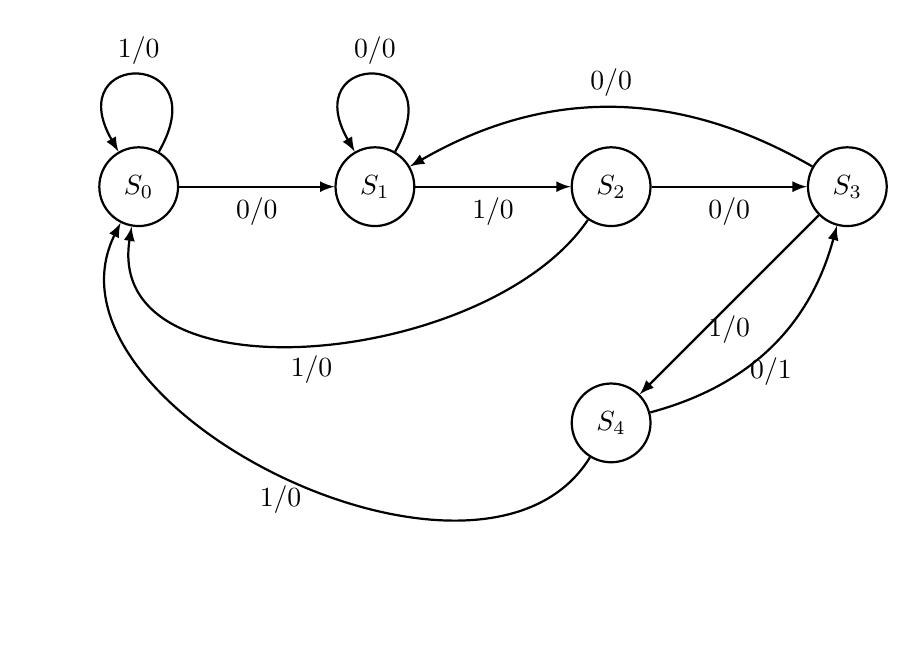
\begin{tikzpicture}[-latex ,node distance=3cm and 1cm,thick,state/.style={circle ,draw, minimum width =1cm}]
  \node[state] (S0) {$S_0$};
  \node[state] (S1) [right of=S0] {$S_1$};
  \node[state] (S2) [right of=S1] {$S_2$};
  \node[state] (S3) [right of=S2] {$S_3$};
  \node[state] (S4) [below of=S2] {$S_4$};

\path (S0) edge [loop above ,out=60, in=120, distance=1.5cm] node {1/0} (S0)
      (S2) edge [bend left , out=55, in=80] node [below=0.15] {1/0} (S0)
      (S1) edge [loop above ,out=60, in=120, distance=1.5cm] node {0/0} (S1)
      (S0)  edge node [below=0.15] {0/0} (S1)
      (S1) edge node [below=0.15] {1/0} (S2)
      (S2) edge  node [below=0.15] {0/0} (S3)
        (S3) edge [bend right] node[above=0.15] {0/0} (S1)
        (S4) edge [bend right] node [below=0.25] {0/1} (S3)
        (S4) edge [bend left=-40 , out=85, in=90] node [below=0.15] {1/0} (S0)
           (S3) edge node [below=0.15] {1/0} (S4);
\end{tikzpicture}


    \caption{State diagram of a sequence detector}
    	
\end{figure}
\begin{enumerate}
\item   the sequence $01010$ is detected.
\item   the sequence $01011$ is detected.
\item   the sequence $01110$ is detected.
\item   the sequence $01001$ is detected.
\end{enumerate}


\item The state transition diagram for the circuit shown is
                         \hfill(GATE-IN2019,39)
\begin{figure}[H]
\centering
\begin{circuitikz}
            \draw (2,2)coordinate(w)--(5,2)coordinate(x)--(5,6)coordinate(x)--(2,6)coordinate(z)--(2,2)coordinate(w);
            \draw (0.85,5.5)--(2,5.5);
            \draw (2,5.5)node[right]{$D$};
            \draw (1,0)--(1,2.5)--(2,2.5);
            \draw (1,-0.5)node[]{$CLK$};
            \draw (2,2.25)--(2.3,2.5)--(2,2.75);
            \draw (5,5.5)node[left]{$Q$}--(8,5.5)node[right]{$1$};
            \draw (5,2.5)node[left]{$\overline{Q}$}--(8,2.5)node[right]{$0$};
              % Reversed NAND gate (horizontally flipped)
    \draw (5,8) node[nand port,scale=-1] (nand) {};
    %\draw (nand.in 1) node[left] {};
%\draw (nand.in 2) node[left] {};
    
    % Output
    
    \draw (nand.out) -- ++(-4,0) -- ++(0,-2.5) node[above]{};
    % Inputs
    \draw (nand.in 1) -- ++(0,-2.2) node[below]{};
    \draw (nand.in 2) -- ++(4,0)--++(0,-4.2)--++(-0.86,0) node[below]{};
    \draw (8,2)--(8,6)--(9.5,5)--(9.5,3)--(8,2);
    \draw [->](9,0)node[right]{$A$}--(9,2.7);
    
\end{circuitikz}

\caption{Circuit~Diagram}
\end{figure}

\begin{enumerate}
%% options1
\item 
\begin{figure}[H]
\centering
\begin{circuitikz}
[-latex ,node distance=4cm and 2cm,thick,state/.style={circle,draw, minimum width =1cm}] 

\node[state] (Q0) {$Q=0$};
\node[state] (Q1) [right of=Q0]{$Q=1$};
\path (Q0) edge [bend left] node [above=0.15] {A = 1} (Q1);
\path (Q0) edge [loop above ,out=100 ,in=150,distance=2cm] node {A = 0} (Q0);
\path  (Q1) edge [bend left] node [below=0.15] {A = 1} (Q0);
\path (Q1) edge [loop above ,in=60,out=120,distance=2cm] node {A=0} (Q1);
        
\end{circuitikz}


\end{figure}
%% options2
\item \begin{figure}[H]
\centering
\input{ide/fsm/figs/opt2.tex}
\end{figure}
%% options3
\item 
\begin{figure}[H]
\centering
\input{ide/fsm/figs/opt3.tex}
\end{figure}
%% options4
\item 
\begin{figure}[H]
\centering
\input{ide/fsm/figs/opt4.tex}
\end{figure}

\end{enumerate}
\item An $8085$ microprocessor accesses two memory locations $\brak{2001H}$ and $\brak{2002H}$, that contain $8$-bit numbers $98$H and $B1$H, respectively.The following program is executed:
\begin{verbatim}LXI H,2001H
MVI A,21H
INX H
ADD M
INX H
MOV M,A
HLT
\end{verbatim}
At the end of this program, the memory location $2003$H contains the number in decimal $\brak{base 10}$ form $\underline{\hspace{2cm}}$.

$\hfill\brak{GATE\enspace EE2020-54}$

\item A sequence detector is designed to detect precisely $3$ digital inputs, with overlapping sequences detectable. For the sequence $\brak{1,0,1}$ and input data $\brak{1,1,0,1,0,0,1,1,0,1,0,1,1,0}$.
$\hfill\brak{GATE\enspace EE2020-15}$
   \begin{enumerate}
  \item  $\brak{1,1,0,0,0,0,1,1,0,1,0,0}$
  \item $\brak{0,1,0,0,0,0,0,1,0,1,0,0}$
  \item $\brak{0,1,0,0,0,0,0,1,0,1,1,0}$
  \item $\brak{0,1,0,0,0,0,0,0,1,0,0,0}$

\end{enumerate}
\item A $16$-bit synchronous binary up-counter is clocked with the frequency $\vec{f}_{\text{CLK}}$. The two most significant bits are $\vec{OR}$-ed together to form an output $Y$. Measurements show that $Y$ is periodic, and the duration for which $Y$ remains high in each period is $24$ ms. The clock frequency\underline{\hspace{2cm}}MHz.\\ {(Round off to $2$ decimal places.)}
\hfill{\brak{GATE \enspace EE2021-22}}


\item  which of the following is the correct binary equivalent of the hexadecimal F6C?
$\hfill\brak{GATE\enspace PH2020,6}$

\begin{enumerate}
  \item  $0110 1111 1100$
  \item $1111 0110 1100$
  \item $1100 0110 1111$
  \item $0110 1100 0111$

\end{enumerate}

\item P, Q, and R arethe decimal integers corresponding to the  $4$-bit binary number  $1100$ consider in single magnitude, $1$'s complement, and $2$'s complement representations, respectively. The $6$-bit $2$'s complement representation of $\brak{P + Q + R}$ is

   \hfill(GATE EC-2020,38)
\begin{enumerate}
  \item $110101$
  \item $110010$
  \item $111101$
  \item $111001$
\end{enumerate}

\item A finite state machine (FSM) is implemented using the D flip-flops $A$ and $B$, and logic gates, as shown in the figure below. The four possible states of the FSM are $Q_AQ_B = 00, 01, 10$ and	 $11$.  

	\begin{figure}[!ht]
\centering
\resizebox{1\textwidth}{!}{%
\begin{circuitikz}
\tikzstyle{every node}=[font=\Large]

\draw [, line width=0.9pt](4,6) to[short] (17,6);
\draw (4,6) to[short] (17,6);
\draw [, line width=0.9pt ] (5,7) rectangle (9,11);
\draw [, line width=0.9pt ] (15,7) rectangle (19,11);
\draw (11,10) to[short] (11.5,10);
\draw (11,9.5) to[short] (11.5,9.5);
\draw (11.5,10) node[ieeestd nand port, anchor=in 1, scale=0.89](port){} (port.out) to[short] (13.5,9.75);
\draw [, line width=0.9pt](11,9.5) to[short] (11,8.75);
\draw [, line width=0.9pt](9,10) to[short] (11,10);
\draw [, line width=0.9pt](13.5,9.75) to[short] (14,9.75);
\draw [, line width=0.9pt](14,9.75) to[short] (14,10);
\draw [, line width=0.9pt](14,10) to[short] (15,10);
\draw [, line width=0.9pt](19,10) to[short] (20.5,10);
\draw [, line width=0.9pt](20,10) to[short] (20,12);
\draw [, line width=0.9pt](20,12) to[short] (20,13);
\draw[, line width=0.9pt] (20,13) to[short] (10,13);
\draw [, line width=0.9pt](10,10) to[short] (10,12);
\draw (9,13) to[short] (8.75,13);
\draw (9,12.5) to[short] (8.75,12.5);
\draw (8.75,13) node[ieeestd xor port, anchor=in 2, scale=0.89, rotate=180](port){} (port.out) to[short] (6.75,12.75);
\draw[, line width=0.9pt] (10,13) to[short] (8.75,13);
\draw [, line width=0.9pt](10,12) to[short] (10,12.5);
\draw[, line width=0.9pt] (10,12.5) to[short] (9,12.5);
\draw[, line width=0.9pt] (6.75,12.75) to[short] (4,12.75);
\draw [, line width=0.9pt](4,12.75) to[short] (4,10);
\draw [, line width=0.9pt](4,10) to[short] (5,10);
\node [font=\Large] at (7,9) {A};
\node [font=\Large] at (17,9) {B};
\node [font=\Large] at (5.25,10) {D};
\node [font=\Large] at (15.25,10) {D};
\node [font=\Large] at (18.5,10) {Q};
\node [font=\Large] at (8.5,10) {Q};
\node [font=\Large] at (8.5,8) {$\bar Q$};
\node [font=\Large] at (18.5,8) {$\bar Q$};
\node [font=\Large] at (6,7.75) {CK};
\node [font=\Large] at (16,8) {CK};
\node [font=\Large] at (3.25,6) {CLK};
\node [font=\Large] at (11,8.5) {Xin};
\draw [, line width=0.9pt](6.75,6) to[short] (6.75,7);
\draw [, line width=0.9pt](17,6) to[short] (17,7);
\draw [line width=0.9pt, short] (6.25,7) -- (6.75,7.75);
\draw [line width=0.9pt, short] (6.75,7.75) -- (7.25,7);
\draw [line width=0.9pt, short] (16.5,7) -- (17,7.75);
\draw [line width=0.9pt, short] (17,7.75) -- (17.5,7);
\node [font=\Large] at (11.5,10.5) {$Q_A$};
\node [font=\Large] at (20.25,9.5) {$Q_B$};
\end{circuitikz}
}%

\label{fig:ide/fsm/figs/circuit}
\end{figure}

Assume that $X_{IN}$ is held at a constant logic level throughout the operation of the FSM. When the FSM is initialized to the state $Q_AQ_B = 00$ and clocked, after a few clock cycles, it starts cycling through
\begin{enumerate}
\item all of the four possible states if $X_{IN} = 1$
\item three of the four possible states if $X_{IN} = 0$
\item only two of the four possible states if $X_{IN} = 1$
\item only two of the four possible states if $X_{IN} = 0$
\end{enumerate}
\hfill{(GATE EC 2017)}

\end{enumerate}
\item Three particles are to be distributed in four non-degenerate energy levels.The possible number of ways of distribution: (i) For distinguishable particles, and (ii) For identical Bosons,respectively,is\\



\textbf{(A)} (i) 24,(ii) 4 \hfill
\textbf{(B)} (i) 24,(ii) 20 \hfill
\textbf{(C)} (i) 64,(ii) 20 \hfill
\textbf{(D)} (i) 64,(ii) 16
\\

\hfill
\begin{minipage}{0.3\textwidth}
  \raggedleft % 
  \text{(GATE-PH2018)}
\end{minipage}
\end{enumerate}


\chapter{Assembly Programming}
\iffalse
\documentclass[journal,12pt,twocolumn]{IEEEtran}
%
\usepackage{setspace}
\usepackage{gensymb}
%\doublespacing
\singlespacing

%\usepackage{graphicx}
%\usepackage{amssymb}
%\usepackage{relsize}
\usepackage[cmex10]{amsmath}
\usepackage{siunitx}
%\usepackage{amsthm}
%\interdisplaylinepenalty=2500
%\savesymbol{iint}
%\usepackage{txfonts}
%\restoresymbol{TXF}{iint}
%\usepackage{wasysym}
\usepackage{amsthm}
%\usepackage{iithtlc}
\usepackage{mathrsfs}
\usepackage{txfonts}
\usepackage{stfloats}
\usepackage{steinmetz}
\usepackage{supertabular}
%\usepackage{bm}
\usepackage{cite}
\usepackage{cases}
\usepackage{subfig}
%\usepackage{xtab}
\usepackage{longtable}
\usepackage{multirow}
%\usepackage{algorithm}
%\usepackage{algpseudocode}
\usepackage{enumitem}
\usepackage{mathtools}
\usepackage{tikz}
\usepackage{circuitikz}
\usepackage{verbatim}
\usepackage{tfrupee}
\usepackage[breaklinks=true]{hyperref}
%\usepackage{stmaryrd}
\usepackage{tkz-euclide} % loads  TikZ and tkz-base
%\usetkzobj{all}
\usetikzlibrary{calc,math}
\usetikzlibrary{fadings}
\usepackage{listings}
    \usepackage{color}                                            %%
    \usepackage{array}                                            %%
    \usepackage{longtable}                                        %%
    \usepackage{calc}                                             %%
    \usepackage{multirow}                                         %%
    \usepackage{hhline}                                           %%
    \usepackage{ifthen}                                           %%
  %optionally (for landscape tables embedded in another document): %%
    \usepackage{lscape}     
\usepackage{multicol}
\usepackage{chngcntr}
\usepackage{blkarray}
\usepackage{karnaugh-map}
\usepackage{fontspec}
\usepackage[intoc]{nomencl}
\makenomenclature

%\usetikzlibrary{arrows, shapes.gates.logic.US, calc}
\usetikzlibrary{arrows,shapes.gates.logic.US,shapes.gates.logic.IEC,calc}
\setmainfont{Sanskrit_2003.ttf}
%\setmainfont{Nakula.ttf}
%\setmainfont{Lohit-Devanagari.ttf}


%\usepackage{enumerate}

%\usepackage{wasysym}
%\newcounter{MYtempeqncnt}
\DeclareMathOperator*{\Res}{Res}
%\renewcommand{\baselinestretch}{2}
\renewcommand\thesection{\arabic{section}}
\renewcommand\thesubsection{\thesection.\arabic{subsection}}
\renewcommand\thesubsubsection{\thesubsection.\arabic{subsubsection}}

\renewcommand\thesectiondis{\arabic{section}}
\renewcommand\thesubsectiondis{\thesectiondis.\arabic{subsection}}
\renewcommand\thesubsubsectiondis{\thesubsectiondis.\arabic{subsubsection}}

% correct bad hyphenation here
\hyphenation{op-tical net-works semi-conduc-tor}
\def\inputGnumericTable{}                                 %%


\lstset{
%language=shell,
%language = Prolog,
frame=single, 
breaklines=true,
%showstringspaces=false,
columns=fullflexible
literate = {-}{-}1
}
%\lstset{
%language=tex,
%frame=single, 
%breaklines=true
%}

\begin{document}
%


\newtheorem{theorem}{Theorem}[section]
\newtheorem{problem}{Problem}
\newtheorem{proposition}{Proposition}[section]
\newtheorem{lemma}{Lemma}[section]
\newtheorem{corollary}[theorem]{Corollary}
\newtheorem{example}{Example}[section]
\newtheorem{definition}[problem]{Definition}
%\newtheorem{thm}{Theorem}[section] 
%\newtheorem{defn}[thm]{Definition}
%\newtheorem{algorithm}{Algorithm}[section]
%\newtheorem{cor}{Corollary}
\newcommand{\BEQA}{\begin{eqnarray}}
\newcommand{\EEQA}{\end{eqnarray}}
\newcommand{\define}{\stackrel{\triangle}{=}}

\bibliographystyle{IEEEtran}
%\bibliographystyle{ieeetr}


\providecommand{\mbf}{\mathbf}
\providecommand{\pr}[1]{\ensuremath{\Pr\left(#1\right)}}
\providecommand{\qfunc}[1]{\ensuremath{Q\left(#1\right)}}
\providecommand{\sbrak}[1]{\ensuremath{{}\left[#1\right]}}
\providecommand{\lsbrak}[1]{\ensuremath{{}\left[#1\right.}}
\providecommand{\rsbrak}[1]{\ensuremath{{}\left.#1\right]}}
\providecommand{\brak}[1]{\ensuremath{\left(#1\right)}}
\providecommand{\lbrak}[1]{\ensuremath{\left(#1\right.}}
\providecommand{\rbrak}[1]{\ensuremath{\left.#1\right)}}
\providecommand{\cbrak}[1]{\ensuremath{\left\{#1\right\}}}
\providecommand{\lcbrak}[1]{\ensuremath{\left\{#1\right.}}
\providecommand{\rcbrak}[1]{\ensuremath{\left.#1\right\}}}
\providecommand{\ceil}[1]{\left \lceil #1 \right \rceil }
\theoremstyle{remark}
\newtheorem{rem}{Remark}
\newcommand{\sgn}{\mathop{\mathrm{sgn}}}
\providecommand{\abs}[1]{\left\vert#1\right\vert}
\providecommand{\res}[1]{\Res\displaylimits_{#1}} 
\providecommand{\norm}[1]{\left\lVert#1\right\rVert}
%\providecommand{\norm}[1]{\lVert#1\rVert}
\providecommand{\mtx}[1]{\mathbf{#1}}
\providecommand{\mean}[1]{E\left[ #1 \right]}
\providecommand{\fourier}{\overset{\mathcal{F}}{ \rightleftharpoons}}
%\providecommand{\hilbert}{\overset{\mathcal{H}}{ \rightleftharpoons}}
\providecommand{\system}{\overset{\mathcal{H}}{ \longleftrightarrow}}
	%\newcommand{\solution}[2]{\textbf{Solution:}{#1}}
\newcommand{\solution}{\noindent \textbf{Solution: }}
\newcommand{\cosec}{\,\text{cosec}\,}
\providecommand{\dec}[2]{\ensuremath{\overset{#1}{\underset{#2}{\gtrless}}}}
\newcommand{\myvec}[1]{\ensuremath{\begin{pmatrix}#1\end{pmatrix}}}
\newcommand{\mydet}[1]{\ensuremath{\begin{vmatrix}#1\end{vmatrix}}}
%\numberwithin{equation}{section}
\numberwithin{equation}{subsection}
%\numberwithin{problem}{section}
%\numberwithin{definition}{section}
\makeatletter
\@addtoreset{figure}{problem}
\makeatother

\let\StandardTheFigure\thefigure
\let\vec\mathbf
%\renewcommand{\thefigure}{\theproblem.\arabic{figure}}
%\renewcommand{\thefigure}{\theproblem}
\renewcommand{\thefigure}{\thesection}
%\setlist[enumerate,1]{before=\renewcommand\theequation{\theenumi.\arabic{equation}}
%\counterwithin{equation}{enumi}


%\renewcommand{\theequation}{\arabic{subsection}.\arabic{equation}}

\def\putbox#1#2#3{\makebox[0in][l]{\makebox[#1][l]{}\raisebox{\baselineskip}[0in][0in]{\raisebox{#2}[0in][0in]{#3}}}}
     \def\rightbox#1{\makebox[0in][r]{#1}}
     \def\centbox#1{\makebox[0in]{#1}}
     \def\topbox#1{\raisebox{-\baselineskip}[0in][0in]{#1}}
     \def\midbox#1{\raisebox{-0.5\baselineskip}[0in][0in]{#1}}

\vspace{3cm}

\title{
%	\logo{
Digital Design through Vaman
%	}
}
\author{ G. V. V. Sharma $^{*}$% <-this % stops a space
	\thanks{*The author is with the Department of Electrical Engineering, IIT Hyderabad, 502285, India. email: gadepall@ee.iith.ac.in.  All material in this document is released under GNU GPL.  Free to use for anything.}
	
}	
%\title{
%	\logo{Matrix Analysis through Octave}{\begin{center}\includegraphics[scale=.24]{tlc}\end{center}}{}{HAMDSP}
%}


% paper title
% can use linebreaks \\ within to get better formatting as desired
%\title{Matrix Analysis through Octave}
%
%
% author names and IEEE memberships
% note positions of commas and nonbreaking spaces ( ~ ) LaTeX will not break
% a structure at a ~ so this keeps an author's name from being broken across
% two lines.
% use \thanks{} to gain access to the first footnote area
% a separate \thanks must be used for each paragraph as LaTeX2e's \thanks
% was not built to handle multiple paragraphs
%

%\author{<-this % stops a space
%\thanks{}}
%}
% note the % following the last \IEEEmembership and also \thanks - 
% these prevent an unwanted space from occurring between the last author name
% and the end of the author line. i.e., if you had this:
% 
% \author{....lastname \thanks{...} \thanks{...} }
%                     ^------------^------------^----Do not want these spaces!
%
% a space would be appended to the last name and could cause every name on that
% line to be shifted left slightly. This is one of those "LaTeX things". For
% instance, "\textbf{A} \textbf{B}" will typeset as "A B" not "AB". To get
% "AB" then you have to do: "\textbf{A}\textbf{B}"
% \thanks is no different in this regard, so shield the last } of each \thanks
% that ends a line with a % and do not let a space in before the next \thanks.
% Spaces after \IEEEmembership other than the last one are OK (and needed) as
% you are supposed to have spaces between the names. For what it is worth,
% this is a minor point as most people would not even notice if the said evil
% space somehow managed to creep in.



% The paper headers
%\markboth{Journal of \LaTeX\ Class Files,~Vol.~6, No.~1, January~2007}%
%{Shell \MakeLowercase{\textit{et al.}}: Bare Demo of IEEEtran.cls for Journals}
% The only time the second header will appear is for the odd numbered pages
% after the title page when using the twoside option.
% 
% *** Note that you probably will NOT want to include the author's ***
% *** name in the headers of peer review papers.                   ***
% You can use \ifCLASSOPTIONpeerreview for conditional compilation here if
% you desire.




% If you want to put a publisher's ID mark on the page you can do it like
% this:
%\IEEEpubid{0000--0000/00\$00.00~\copyright~2007 IEEE}
% Remember, if you use this you must call \IEEEpubidadjcol in the second
% column for its text to clear the IEEEpubid mark.



% make the title area
\maketitle

\newpage

\tableofcontents


\bigskip

\renewcommand{\thefigure}{\theenumi}
\renewcommand{\thetable}{\theenumi}
%\renewcommand{\abstractname}{सार}
%\renewcommand{\nomname}{नामकरण}
%\renewcommand{\solution}{हल: }
%\renewcommand{\figurename}{आकृति.}
%\renewcommand{\tablename}{सारणी.}
%\renewcommand{\theequation}{\theenumi}

%\begin{abstract}
%%\boldmath
%In this letter, an algorithm for evaluating the exact analytical bit error rate  (BER)  for the piecewise linear (PL) combiner for  multiple relays is presented. Previous results were available only for upto three relays. The algorithm is unique in the sense that  the actual mathematical expressions, that are prohibitively large, need not be explicitly obtained. The diversity gain due to multiple relays is shown through plots of the analytical BER, well supported by simulations. 
%
%\end{abstract}
% IEEEtran.cls defaults to using nonbold math in the Abstract.
% This preserves the distinction between vectors and scalars. However,
% if the journal you are submitting to favors bold math in the abstract,
% then you can use LaTeX's standard command \boldmath at the very start
% of the abstract to achieve this. Many IEEE journals frown on math
% in the abstract anyway.

% Note that keywords are not normally used for peerreview papers.
%\begin{IEEEkeywords}
%Cooperative diversity, decode and forward, piecewise linear
%\end{IEEEkeywords}



% For peer review papers, you can put extra information on the cover
% page as needed:
% \ifCLASSOPTIONpeerreview
% \begin{center} \bfseries EDICS Category: 3-BBND \end{center}
% \fi
%
% For peerreview papers, this IEEEtran command inserts a page break and
% creates the second title. It will be ignored for other modes.
%\IEEEpeerreviewmaketitle
\fi

\begin{abstract}
The objective of this manual is to introduce beginners to arm embedded programming by powering a seven segment display.
\end{abstract}
\subsection{Components}
\renewcommand{\theequation}{\theenumi}
\renewcommand{\thefigure}{\theenumi}
\begin{enumerate}[label=\thesubsection.\arabic*.,ref=\thesubsection.\theenumi]
\numberwithin{equation}{enumi}
\numberwithin{figure}{enumi}
\numberwithin{table}{enumi}
\item The necessary components for this manual are listed in Table \ref{tabel:stm32/sevenseg/components}.
\begin{table}[!ht]
\begin{center}
\input{./stm32/sevenseg/figs/components.tex}
\end{center}
\caption{Components}
\label{tabel:stm32/sevenseg/components}
\end{table}
\subsection{Hardware}

%\subsection{Seven Segment Display}
%The breadboard can be divided into 5 segments.  In each of the green segements, the pins are internally connected so as to have the same voltage.  Similarly, in the central segments, the pins in each column  are internally connected in the same fashion as the blue columns. 

%\begin{problem}
%	Plug the display to the breadboard in Fig. \ref{fig:breadboard}
%\end{problem}
%\begin{figure}[!h]
%\begin{center}
%\includegraphics[width=\columnwidth]{./figs/breadboard}
%\end{center}
%\caption{}
%\label{fig:breadboard}
%\end{figure}
\item The seven segment display in Fig. \ref{fig:sevenseg} has eight pins, $a, b, c, d, e, f, g$ and $dot$ that take an active LOW input, i.e.  the LED will glow only if the input is connected to ground.  Each of these pins is connected to an LED segment.  The $dot$ pin is  reserved for the $\cdot$ LED.  

%
%\begin{center}
	%\includegraphics[scale=1]{sevenseg}
%\end{center}


\item Connect one end of the 1K resistor to the COM pin of the display and the other end to an extreme pin of the breadboard.	
%
%
%
%\begin{figure}[!h]
%\begin{center}
%\resizebox {0.5\columnwidth} {!} {
%\input{./figs/sevenseg.tex}
%}
%\end{center}
%\caption{}
%\label{fig:sevenseg}
%\end{figure}

\item The STM32F103C8T6 micro-controller in Fig. \ref{fig:stm_blue} has two ground pins, few analog input pins and few digital pins that can be used for both input as well as output. It has one Vcc (3.3V) pin that can generate 3.3$V$.  In the following exercises, only the GND, 3.3$V$ and digital pins will be used.
%
%
\item Make the pin connections in Table \ref{table:stm_ssd} using Figs. \ref{fig:sevenseg} and \ref{fig:stm_blue}.
	
%
\begin{figure}[!h]
\begin{center}
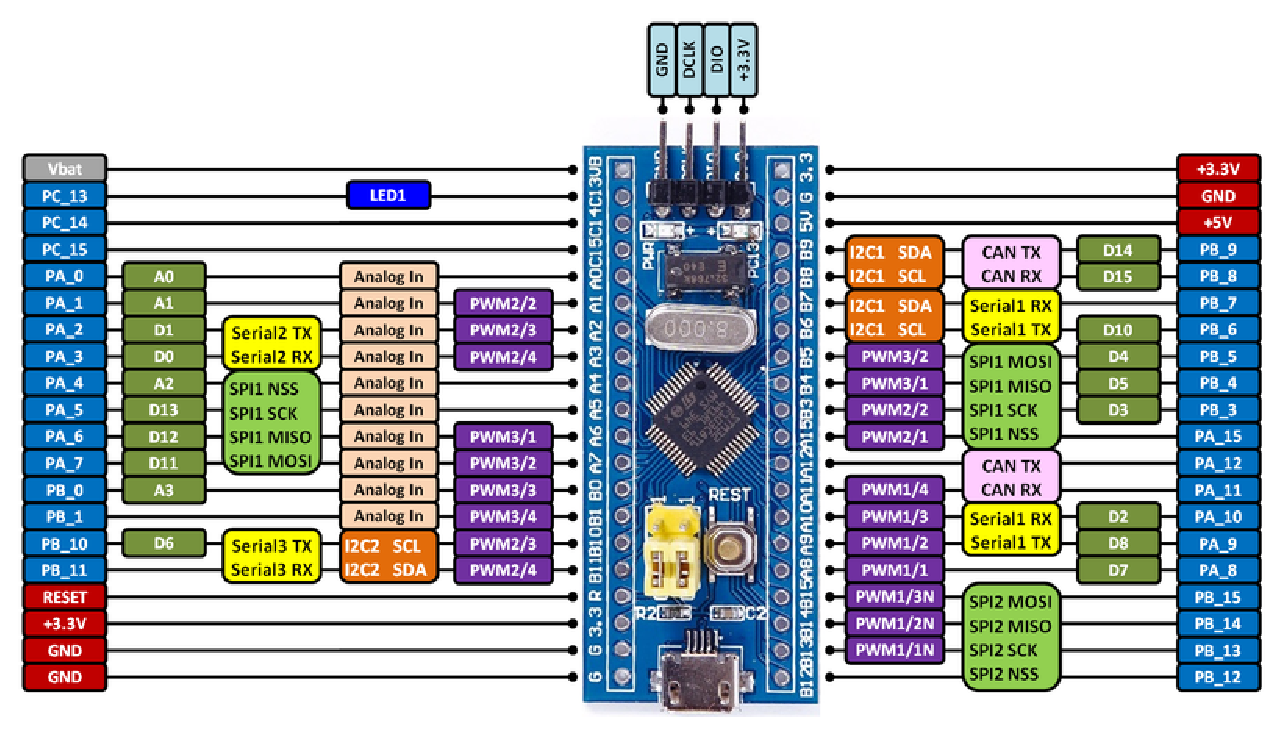
\includegraphics[width=\columnwidth]{./stm32/sevenseg/figs/stm_blue.eps}
\end{center}
\caption{Pin Connections of STM-32}
\label{fig:stm_blue}
\end{figure}
%
\begin{table}
\begin{center}
\input{./stm32/sevenseg/figs/stm_ssd}
\end{center}
\caption{STM-32 and Seven Segment Display Connections}
\label{table:stm_ssd}
\end{table}

\subsection{Software}
%
\item Before flashing code to STM32 set the STM32 board to Programming mode as shown in Fig. \ref{fig:programming_mode}, then change the mode to Operating mode as shown in Fig. \ref{fig:programming_mode} after flashing the code inorder to run your program from main memory.
\item Execute the following code 
\begin{lstlisting}
cd stm32/sevenseg/codes/sevenseg_example.c
\end{lstlisting}

%\begin{problem}
%	Connect the STM32 to the Raspberry Pi according to the \href{https://github.com/gadepall/EE4013/blob/master/setup/rpi/gvv_stm32_setup.pdf}{\url{instructions }} in
%\begin{lstlisting}
%https://github.com/gadepall/EE4013/blob/master/setup/rpi/gvv_stm32_setup.pdf
%\end{lstlisting}	
%\end{problem}
%\section{Display Control with STM32}
%
%\begin{problem}
%Follow the \href{https://github.com/gadepall/EE4013/blob/master/setup/tinker/gvv_stm32_tinker_setup.pdf}{\url{instructions }} in
%\begin{lstlisting}
%https://github.com/gadepall/EE4013/blob/master/setup/tinker/gvv_stm32_tinker_setup.pdf
%\end{lstlisting}
%to clone the \href{https://github.com/gadepall/EE4013/blob/master/setup/tinker/gvv_stm32_tinker_setup.pdf}{\url{repository }}
%\begin{lstlisting}[language=bash, frame=single, breaklines]
%https://github.com/gadepall/STM32F103C8T6
%\end{lstlisting}
%\end{problem}
%
%Fig. \ref{fig:sevenseg12} explains how to get decimal digits using the seven segment display. 
%\begin{problem}
%In the STM32F103C8T6 directory,
%\begin{lstlisting}
%cp sevenseg.c main.c
%\end{lstlisting}
%Generate the number 0 by executing \textbf{main.c} and flashing to the STM32. 
%\end{problem}	
%
%\begin{figure}[!h]
%\begin{center}
%\resizebox {0.8\columnwidth} {!} {
%\input{./figs/sevenseg12.tex}
%}
%\end{center}
%\caption{}
%\label{fig:sevenseg12}
%\end{figure}
%

\item Explain the process of generating the number 0 using the following instruction.
\begin{lstlisting}
GPIOB->ODR = 0xFC08;
\end{lstlisting}
\solution ODR is the Output Data Register, which is used to write outputs to the GPIO pins. The 16 bit number 0xFC08 on the RHS represents the pin configuration for the pins of port B of STM32F103C8T6, which are numbered PB15-PB0 in that order.  See Table \ref{table:stm_ssd}.
\\
\item Repeat the above exercise to generate the numbers 1-9 on the display.
\item The previous instructions set the bits in the unused ports PB15-PB10 and PB2-PB0. This may be undesirable in some cases. Generate 0 by not disturbing 
the unused pins.
\\
\solution The following instructions help accomplish this. The first instruction resets PB4-PB9.  The second instruction sets the PB3 pin. The other pins are
undisturbed.
\begin{lstlisting}
GPIOB->BRR = (1<<4)|(1<<5)|(1<<6)|(1<<7)|(1<<8)|(1<<9); // (Led ON)		
GPIOB->BSRR = (1<<3); // (Led OFF)					
\end{lstlisting}
%\section{Manual Display Control}
%\input{./chapters/chapter1}
%
\item Write a program to take a 4-bit BCD as input from hardware (GND or VDD) and show the next number on the seven segment display.
\\
\solution The following program takes 4 bits as input from pins PB12-PB15 and displays the output on a seven segment display. The next number
can be displayed by slightly modifying the code.
\begin{lstlisting}
cd codes/bin2dec_example.c
\end{lstlisting}
\end{enumerate}

\iffalse
\documentclass[journal,12pt,twocolumn]{IEEEtran}
%
\usepackage{setspace}
\usepackage{gensymb}
%\doublespacing
\singlespacing

%\usepackage{graphicx}
%\usepackage{amssymb}
%\usepackage{relsize}
\usepackage[cmex10]{amsmath}
\usepackage{siunitx}
%\usepackage{amsthm}
%\interdisplaylinepenalty=2500
%\savesymbol{iint}
%\usepackage{txfonts}
%\restoresymbol{TXF}{iint}
%\usepackage{wasysym}
\usepackage{amsthm}
%\usepackage{iithtlc}
\usepackage{mathrsfs}
\usepackage{txfonts}
\usepackage{stfloats}
\usepackage{steinmetz}
\usepackage{supertabular}
%\usepackage{bm}
\usepackage{cite}
\usepackage{cases}
\usepackage{subfig}
%\usepackage{xtab}
\usepackage{longtable}
\usepackage{multirow}
%\usepackage{algorithm}
%\usepackage{algpseudocode}
\usepackage{enumitem}
\usepackage{mathtools}
\usepackage{tikz}
\usepackage{circuitikz}
\usepackage{verbatim}
\usepackage{tfrupee}
\usepackage[breaklinks=true]{hyperref}
%\usepackage{stmaryrd}
\usepackage{tkz-euclide} % loads  TikZ and tkz-base
%\usetkzobj{all}
\usetikzlibrary{calc,math}
\usetikzlibrary{fadings}
\usepackage{listings}
    \usepackage{color}                                            %%
    \usepackage{array}                                            %%
    \usepackage{longtable}                                        %%
    \usepackage{calc}                                             %%
    \usepackage{multirow}                                         %%
    \usepackage{hhline}                                           %%
    \usepackage{ifthen}                                           %%
  %optionally (for landscape tables embedded in another document): %%
    \usepackage{lscape}     
\usepackage{multicol}
\usepackage{chngcntr}
\usepackage{blkarray}
\usepackage{karnaugh-map}
\usepackage{fontspec}
\usepackage[intoc]{nomencl}
\makenomenclature

%\usetikzlibrary{arrows, shapes.gates.logic.US, calc}
\usetikzlibrary{arrows,shapes.gates.logic.US,shapes.gates.logic.IEC,calc}
\setmainfont{Sanskrit_2003.ttf}
%\setmainfont{Nakula.ttf}
%\setmainfont{Lohit-Devanagari.ttf}


%\usepackage{enumerate}

%\usepackage{wasysym}
%\newcounter{MYtempeqncnt}
\DeclareMathOperator*{\Res}{Res}
%\renewcommand{\baselinestretch}{2}
\renewcommand\thesection{\arabic{section}}
\renewcommand\thesubsection{\thesection.\arabic{subsection}}
\renewcommand\thesubsubsection{\thesubsection.\arabic{subsubsection}}

\renewcommand\thesectiondis{\arabic{section}}
\renewcommand\thesubsectiondis{\thesectiondis.\arabic{subsection}}
\renewcommand\thesubsubsectiondis{\thesubsectiondis.\arabic{subsubsection}}

% correct bad hyphenation here
\hyphenation{op-tical net-works semi-conduc-tor}
\def\inputGnumericTable{}                                 %%


\lstset{
%language=shell,
%language = Prolog,
frame=single, 
breaklines=true,
%showstringspaces=false,
columns=fullflexible
literate = {-}{-}1
}
%\lstset{
%language=tex,
%frame=single, 
%breaklines=true
%}

\begin{document}
%


\newtheorem{theorem}{Theorem}[section]
\newtheorem{problem}{Problem}
\newtheorem{proposition}{Proposition}[section]
\newtheorem{lemma}{Lemma}[section]
\newtheorem{corollary}[theorem]{Corollary}
\newtheorem{example}{Example}[section]
\newtheorem{definition}[problem]{Definition}
%\newtheorem{thm}{Theorem}[section] 
%\newtheorem{defn}[thm]{Definition}
%\newtheorem{algorithm}{Algorithm}[section]
%\newtheorem{cor}{Corollary}
\newcommand{\BEQA}{\begin{eqnarray}}
\newcommand{\EEQA}{\end{eqnarray}}
\newcommand{\define}{\stackrel{\triangle}{=}}

\bibliographystyle{IEEEtran}
%\bibliographystyle{ieeetr}


\providecommand{\mbf}{\mathbf}
\providecommand{\pr}[1]{\ensuremath{\Pr\left(#1\right)}}
\providecommand{\qfunc}[1]{\ensuremath{Q\left(#1\right)}}
\providecommand{\sbrak}[1]{\ensuremath{{}\left[#1\right]}}
\providecommand{\lsbrak}[1]{\ensuremath{{}\left[#1\right.}}
\providecommand{\rsbrak}[1]{\ensuremath{{}\left.#1\right]}}
\providecommand{\brak}[1]{\ensuremath{\left(#1\right)}}
\providecommand{\lbrak}[1]{\ensuremath{\left(#1\right.}}
\providecommand{\rbrak}[1]{\ensuremath{\left.#1\right)}}
\providecommand{\cbrak}[1]{\ensuremath{\left\{#1\right\}}}
\providecommand{\lcbrak}[1]{\ensuremath{\left\{#1\right.}}
\providecommand{\rcbrak}[1]{\ensuremath{\left.#1\right\}}}
\providecommand{\ceil}[1]{\left \lceil #1 \right \rceil }
\theoremstyle{remark}
\newtheorem{rem}{Remark}
\newcommand{\sgn}{\mathop{\mathrm{sgn}}}
\providecommand{\abs}[1]{\left\vert#1\right\vert}
\providecommand{\res}[1]{\Res\displaylimits_{#1}} 
\providecommand{\norm}[1]{\left\lVert#1\right\rVert}
%\providecommand{\norm}[1]{\lVert#1\rVert}
\providecommand{\mtx}[1]{\mathbf{#1}}
\providecommand{\mean}[1]{E\left[ #1 \right]}
\providecommand{\fourier}{\overset{\mathcal{F}}{ \rightleftharpoons}}
%\providecommand{\hilbert}{\overset{\mathcal{H}}{ \rightleftharpoons}}
\providecommand{\system}{\overset{\mathcal{H}}{ \longleftrightarrow}}
	%\newcommand{\solution}[2]{\textbf{Solution:}{#1}}
\newcommand{\solution}{\noindent \textbf{Solution: }}
\newcommand{\cosec}{\,\text{cosec}\,}
\providecommand{\dec}[2]{\ensuremath{\overset{#1}{\underset{#2}{\gtrless}}}}
\newcommand{\myvec}[1]{\ensuremath{\begin{pmatrix}#1\end{pmatrix}}}
\newcommand{\mydet}[1]{\ensuremath{\begin{vmatrix}#1\end{vmatrix}}}
%\numberwithin{equation}{section}
\numberwithin{equation}{subsection}
%\numberwithin{problem}{section}
%\numberwithin{definition}{section}
\makeatletter
\@addtoreset{figure}{problem}
\makeatother

\let\StandardTheFigure\thefigure
\let\vec\mathbf
%\renewcommand{\thefigure}{\theproblem.\arabic{figure}}
%\renewcommand{\thefigure}{\theproblem}
\renewcommand{\thefigure}{\thesection}
%\setlist[enumerate,1]{before=\renewcommand\theequation{\theenumi.\arabic{equation}}
%\counterwithin{equation}{enumi}


%\renewcommand{\theequation}{\arabic{subsection}.\arabic{equation}}

\def\putbox#1#2#3{\makebox[0in][l]{\makebox[#1][l]{}\raisebox{\baselineskip}[0in][0in]{\raisebox{#2}[0in][0in]{#3}}}}
     \def\rightbox#1{\makebox[0in][r]{#1}}
     \def\centbox#1{\makebox[0in]{#1}}
     \def\topbox#1{\raisebox{-\baselineskip}[0in][0in]{#1}}
     \def\midbox#1{\raisebox{-0.5\baselineskip}[0in][0in]{#1}}

\vspace{3cm}

\title{
%	\logo{
Digital Design through Vaman
%	}
}
\author{ G. V. V. Sharma $^{*}$% <-this % stops a space
	\thanks{*The author is with the Department of Electrical Engineering, IIT Hyderabad, 502285, India. email: gadepall@ee.iith.ac.in.  All material in this document is released under GNU GPL.  Free to use for anything.}
	
}	
%\title{
%	\logo{Matrix Analysis through Octave}{\begin{center}\includegraphics[scale=.24]{tlc}\end{center}}{}{HAMDSP}
%}


% paper title
% can use linebreaks \\ within to get better formatting as desired
%\title{Matrix Analysis through Octave}
%
%
% author names and IEEE memberships
% note positions of commas and nonbreaking spaces ( ~ ) LaTeX will not break
% a structure at a ~ so this keeps an author's name from being broken across
% two lines.
% use \thanks{} to gain access to the first footnote area
% a separate \thanks must be used for each paragraph as LaTeX2e's \thanks
% was not built to handle multiple paragraphs
%

%\author{<-this % stops a space
%\thanks{}}
%}
% note the % following the last \IEEEmembership and also \thanks - 
% these prevent an unwanted space from occurring between the last author name
% and the end of the author line. i.e., if you had this:
% 
% \author{....lastname \thanks{...} \thanks{...} }
%                     ^------------^------------^----Do not want these spaces!
%
% a space would be appended to the last name and could cause every name on that
% line to be shifted left slightly. This is one of those "LaTeX things". For
% instance, "\textbf{A} \textbf{B}" will typeset as "A B" not "AB". To get
% "AB" then you have to do: "\textbf{A}\textbf{B}"
% \thanks is no different in this regard, so shield the last } of each \thanks
% that ends a line with a % and do not let a space in before the next \thanks.
% Spaces after \IEEEmembership other than the last one are OK (and needed) as
% you are supposed to have spaces between the names. For what it is worth,
% this is a minor point as most people would not even notice if the said evil
% space somehow managed to creep in.



% The paper headers
%\markboth{Journal of \LaTeX\ Class Files,~Vol.~6, No.~1, January~2007}%
%{Shell \MakeLowercase{\textit{et al.}}: Bare Demo of IEEEtran.cls for Journals}
% The only time the second header will appear is for the odd numbered pages
% after the title page when using the twoside option.
% 
% *** Note that you probably will NOT want to include the author's ***
% *** name in the headers of peer review papers.                   ***
% You can use \ifCLASSOPTIONpeerreview for conditional compilation here if
% you desire.




% If you want to put a publisher's ID mark on the page you can do it like
% this:
%\IEEEpubid{0000--0000/00\$00.00~\copyright~2007 IEEE}
% Remember, if you use this you must call \IEEEpubidadjcol in the second
% column for its text to clear the IEEEpubid mark.



% make the title area
\maketitle

\newpage

\tableofcontents


\bigskip

\renewcommand{\thefigure}{\theenumi}
\renewcommand{\thetable}{\theenumi}
%\renewcommand{\abstractname}{सार}
%\renewcommand{\nomname}{नामकरण}
%\renewcommand{\solution}{हल: }
%\renewcommand{\figurename}{आकृति.}
%\renewcommand{\tablename}{सारणी.}
%\renewcommand{\theequation}{\theenumi}

%\begin{abstract}
%%\boldmath
%In this letter, an algorithm for evaluating the exact analytical bit error rate  (BER)  for the piecewise linear (PL) combiner for  multiple relays is presented. Previous results were available only for upto three relays. The algorithm is unique in the sense that  the actual mathematical expressions, that are prohibitively large, need not be explicitly obtained. The diversity gain due to multiple relays is shown through plots of the analytical BER, well supported by simulations. 
%
%\end{abstract}
% IEEEtran.cls defaults to using nonbold math in the Abstract.
% This preserves the distinction between vectors and scalars. However,
% if the journal you are submitting to favors bold math in the abstract,
% then you can use LaTeX's standard command \boldmath at the very start
% of the abstract to achieve this. Many IEEE journals frown on math
% in the abstract anyway.

% Note that keywords are not normally used for peerreview papers.
%\begin{IEEEkeywords}
%Cooperative diversity, decode and forward, piecewise linear
%\end{IEEEkeywords}



% For peer review papers, you can put extra information on the cover
% page as needed:
% \ifCLASSOPTIONpeerreview
% \begin{center} \bfseries EDICS Category: 3-BBND \end{center}
% \fi
%
% For peerreview papers, this IEEEtran command inserts a page break and
% creates the second title. It will be ignored for other modes.
%\IEEEpeerreviewmaketitle
\fi

\begin{abstract}
The objective of this manual is to introduce beginners to arm embedded programming by powering a seven segment display.
\end{abstract}
\subsection{Components}
\renewcommand{\theequation}{\theenumi}
\renewcommand{\thefigure}{\theenumi}
\begin{enumerate}[label=\thesubsection.\arabic*.,ref=\thesubsection.\theenumi]
\numberwithin{equation}{enumi}
\numberwithin{figure}{enumi}
\numberwithin{table}{enumi}
\item The necessary components for this manual are listed in Table \ref{tabel:stm32/sevenseg/components}.
\begin{table}[!ht]
\begin{center}
\input{./stm32/sevenseg/figs/components.tex}
\end{center}
\caption{Components}
\label{tabel:stm32/sevenseg/components}
\end{table}
\subsection{Hardware}

%\subsection{Seven Segment Display}
%The breadboard can be divided into 5 segments.  In each of the green segements, the pins are internally connected so as to have the same voltage.  Similarly, in the central segments, the pins in each column  are internally connected in the same fashion as the blue columns. 

%\begin{problem}
%	Plug the display to the breadboard in Fig. \ref{fig:breadboard}
%\end{problem}
%\begin{figure}[!h]
%\begin{center}
%\includegraphics[width=\columnwidth]{./figs/breadboard}
%\end{center}
%\caption{}
%\label{fig:breadboard}
%\end{figure}
\item The seven segment display in Fig. \ref{fig:sevenseg} has eight pins, $a, b, c, d, e, f, g$ and $dot$ that take an active LOW input, i.e.  the LED will glow only if the input is connected to ground.  Each of these pins is connected to an LED segment.  The $dot$ pin is  reserved for the $\cdot$ LED.  

%
%\begin{center}
	%\includegraphics[scale=1]{sevenseg}
%\end{center}


\item Connect one end of the 1K resistor to the COM pin of the display and the other end to an extreme pin of the breadboard.	
%
%
%
%\begin{figure}[!h]
%\begin{center}
%\resizebox {0.5\columnwidth} {!} {
%\input{./figs/sevenseg.tex}
%}
%\end{center}
%\caption{}
%\label{fig:sevenseg}
%\end{figure}

\item The STM32F103C8T6 micro-controller in Fig. \ref{fig:stm_blue} has two ground pins, few analog input pins and few digital pins that can be used for both input as well as output. It has one Vcc (3.3V) pin that can generate 3.3$V$.  In the following exercises, only the GND, 3.3$V$ and digital pins will be used.
%
%
\item Make the pin connections in Table \ref{table:stm_ssd} using Figs. \ref{fig:sevenseg} and \ref{fig:stm_blue}.
	
%
\begin{figure}[!h]
\begin{center}
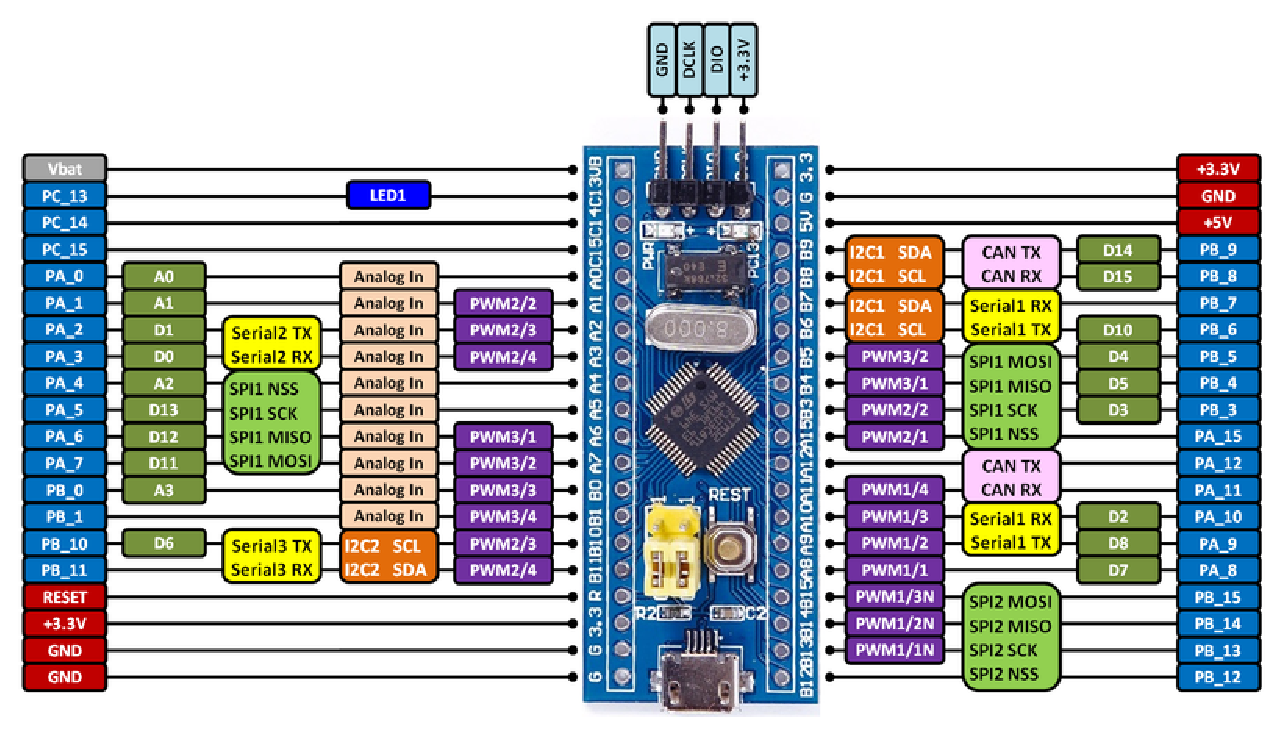
\includegraphics[width=\columnwidth]{./stm32/sevenseg/figs/stm_blue.eps}
\end{center}
\caption{Pin Connections of STM-32}
\label{fig:stm_blue}
\end{figure}
%
\begin{table}
\begin{center}
\input{./stm32/sevenseg/figs/stm_ssd}
\end{center}
\caption{STM-32 and Seven Segment Display Connections}
\label{table:stm_ssd}
\end{table}

\subsection{Software}
%
\item Before flashing code to STM32 set the STM32 board to Programming mode as shown in Fig. \ref{fig:programming_mode}, then change the mode to Operating mode as shown in Fig. \ref{fig:programming_mode} after flashing the code inorder to run your program from main memory.
\item Execute the following code 
\begin{lstlisting}
cd stm32/sevenseg/codes/sevenseg_example.c
\end{lstlisting}

%\begin{problem}
%	Connect the STM32 to the Raspberry Pi according to the \href{https://github.com/gadepall/EE4013/blob/master/setup/rpi/gvv_stm32_setup.pdf}{\url{instructions }} in
%\begin{lstlisting}
%https://github.com/gadepall/EE4013/blob/master/setup/rpi/gvv_stm32_setup.pdf
%\end{lstlisting}	
%\end{problem}
%\section{Display Control with STM32}
%
%\begin{problem}
%Follow the \href{https://github.com/gadepall/EE4013/blob/master/setup/tinker/gvv_stm32_tinker_setup.pdf}{\url{instructions }} in
%\begin{lstlisting}
%https://github.com/gadepall/EE4013/blob/master/setup/tinker/gvv_stm32_tinker_setup.pdf
%\end{lstlisting}
%to clone the \href{https://github.com/gadepall/EE4013/blob/master/setup/tinker/gvv_stm32_tinker_setup.pdf}{\url{repository }}
%\begin{lstlisting}[language=bash, frame=single, breaklines]
%https://github.com/gadepall/STM32F103C8T6
%\end{lstlisting}
%\end{problem}
%
%Fig. \ref{fig:sevenseg12} explains how to get decimal digits using the seven segment display. 
%\begin{problem}
%In the STM32F103C8T6 directory,
%\begin{lstlisting}
%cp sevenseg.c main.c
%\end{lstlisting}
%Generate the number 0 by executing \textbf{main.c} and flashing to the STM32. 
%\end{problem}	
%
%\begin{figure}[!h]
%\begin{center}
%\resizebox {0.8\columnwidth} {!} {
%\input{./figs/sevenseg12.tex}
%}
%\end{center}
%\caption{}
%\label{fig:sevenseg12}
%\end{figure}
%

\item Explain the process of generating the number 0 using the following instruction.
\begin{lstlisting}
GPIOB->ODR = 0xFC08;
\end{lstlisting}
\solution ODR is the Output Data Register, which is used to write outputs to the GPIO pins. The 16 bit number 0xFC08 on the RHS represents the pin configuration for the pins of port B of STM32F103C8T6, which are numbered PB15-PB0 in that order.  See Table \ref{table:stm_ssd}.
\\
\item Repeat the above exercise to generate the numbers 1-9 on the display.
\item The previous instructions set the bits in the unused ports PB15-PB10 and PB2-PB0. This may be undesirable in some cases. Generate 0 by not disturbing 
the unused pins.
\\
\solution The following instructions help accomplish this. The first instruction resets PB4-PB9.  The second instruction sets the PB3 pin. The other pins are
undisturbed.
\begin{lstlisting}
GPIOB->BRR = (1<<4)|(1<<5)|(1<<6)|(1<<7)|(1<<8)|(1<<9); // (Led ON)		
GPIOB->BSRR = (1<<3); // (Led OFF)					
\end{lstlisting}
%\section{Manual Display Control}
%\input{./chapters/chapter1}
%
\item Write a program to take a 4-bit BCD as input from hardware (GND or VDD) and show the next number on the seven segment display.
\\
\solution The following program takes 4 bits as input from pins PB12-PB15 and displays the output on a seven segment display. The next number
can be displayed by slightly modifying the code.
\begin{lstlisting}
cd codes/bin2dec_example.c
\end{lstlisting}
\end{enumerate}

\iffalse
\documentclass[journal,12pt,twocolumn]{IEEEtran}
%
\usepackage{setspace}
\usepackage{gensymb}
%\doublespacing
\singlespacing

%\usepackage{graphicx}
%\usepackage{amssymb}
%\usepackage{relsize}
\usepackage[cmex10]{amsmath}
\usepackage{siunitx}
%\usepackage{amsthm}
%\interdisplaylinepenalty=2500
%\savesymbol{iint}
%\usepackage{txfonts}
%\restoresymbol{TXF}{iint}
%\usepackage{wasysym}
\usepackage{amsthm}
%\usepackage{iithtlc}
\usepackage{mathrsfs}
\usepackage{txfonts}
\usepackage{stfloats}
\usepackage{steinmetz}
\usepackage{supertabular}
%\usepackage{bm}
\usepackage{cite}
\usepackage{cases}
\usepackage{subfig}
%\usepackage{xtab}
\usepackage{longtable}
\usepackage{multirow}
%\usepackage{algorithm}
%\usepackage{algpseudocode}
\usepackage{enumitem}
\usepackage{mathtools}
\usepackage{tikz}
\usepackage{circuitikz}
\usepackage{verbatim}
\usepackage{tfrupee}
\usepackage[breaklinks=true]{hyperref}
%\usepackage{stmaryrd}
\usepackage{tkz-euclide} % loads  TikZ and tkz-base
%\usetkzobj{all}
\usetikzlibrary{calc,math}
\usetikzlibrary{fadings}
\usepackage{listings}
    \usepackage{color}                                            %%
    \usepackage{array}                                            %%
    \usepackage{longtable}                                        %%
    \usepackage{calc}                                             %%
    \usepackage{multirow}                                         %%
    \usepackage{hhline}                                           %%
    \usepackage{ifthen}                                           %%
  %optionally (for landscape tables embedded in another document): %%
    \usepackage{lscape}     
\usepackage{multicol}
\usepackage{chngcntr}
\usepackage{blkarray}
\usepackage{karnaugh-map}
\usepackage{fontspec}
\usepackage[intoc]{nomencl}
\makenomenclature

%\usetikzlibrary{arrows, shapes.gates.logic.US, calc}
\usetikzlibrary{arrows,shapes.gates.logic.US,shapes.gates.logic.IEC,calc}
\setmainfont{Sanskrit_2003.ttf}
%\setmainfont{Nakula.ttf}
%\setmainfont{Lohit-Devanagari.ttf}


%\usepackage{enumerate}

%\usepackage{wasysym}
%\newcounter{MYtempeqncnt}
\DeclareMathOperator*{\Res}{Res}
%\renewcommand{\baselinestretch}{2}
\renewcommand\thesection{\arabic{section}}
\renewcommand\thesubsection{\thesection.\arabic{subsection}}
\renewcommand\thesubsubsection{\thesubsection.\arabic{subsubsection}}

\renewcommand\thesectiondis{\arabic{section}}
\renewcommand\thesubsectiondis{\thesectiondis.\arabic{subsection}}
\renewcommand\thesubsubsectiondis{\thesubsectiondis.\arabic{subsubsection}}

% correct bad hyphenation here
\hyphenation{op-tical net-works semi-conduc-tor}
\def\inputGnumericTable{}                                 %%


\lstset{
%language=shell,
%language = Prolog,
frame=single, 
breaklines=true,
%showstringspaces=false,
columns=fullflexible
literate = {-}{-}1
}
%\lstset{
%language=tex,
%frame=single, 
%breaklines=true
%}

\begin{document}
%


\newtheorem{theorem}{Theorem}[section]
\newtheorem{problem}{Problem}
\newtheorem{proposition}{Proposition}[section]
\newtheorem{lemma}{Lemma}[section]
\newtheorem{corollary}[theorem]{Corollary}
\newtheorem{example}{Example}[section]
\newtheorem{definition}[problem]{Definition}
%\newtheorem{thm}{Theorem}[section] 
%\newtheorem{defn}[thm]{Definition}
%\newtheorem{algorithm}{Algorithm}[section]
%\newtheorem{cor}{Corollary}
\newcommand{\BEQA}{\begin{eqnarray}}
\newcommand{\EEQA}{\end{eqnarray}}
\newcommand{\define}{\stackrel{\triangle}{=}}

\bibliographystyle{IEEEtran}
%\bibliographystyle{ieeetr}


\providecommand{\mbf}{\mathbf}
\providecommand{\pr}[1]{\ensuremath{\Pr\left(#1\right)}}
\providecommand{\qfunc}[1]{\ensuremath{Q\left(#1\right)}}
\providecommand{\sbrak}[1]{\ensuremath{{}\left[#1\right]}}
\providecommand{\lsbrak}[1]{\ensuremath{{}\left[#1\right.}}
\providecommand{\rsbrak}[1]{\ensuremath{{}\left.#1\right]}}
\providecommand{\brak}[1]{\ensuremath{\left(#1\right)}}
\providecommand{\lbrak}[1]{\ensuremath{\left(#1\right.}}
\providecommand{\rbrak}[1]{\ensuremath{\left.#1\right)}}
\providecommand{\cbrak}[1]{\ensuremath{\left\{#1\right\}}}
\providecommand{\lcbrak}[1]{\ensuremath{\left\{#1\right.}}
\providecommand{\rcbrak}[1]{\ensuremath{\left.#1\right\}}}
\providecommand{\ceil}[1]{\left \lceil #1 \right \rceil }
\theoremstyle{remark}
\newtheorem{rem}{Remark}
\newcommand{\sgn}{\mathop{\mathrm{sgn}}}
\providecommand{\abs}[1]{\left\vert#1\right\vert}
\providecommand{\res}[1]{\Res\displaylimits_{#1}} 
\providecommand{\norm}[1]{\left\lVert#1\right\rVert}
%\providecommand{\norm}[1]{\lVert#1\rVert}
\providecommand{\mtx}[1]{\mathbf{#1}}
\providecommand{\mean}[1]{E\left[ #1 \right]}
\providecommand{\fourier}{\overset{\mathcal{F}}{ \rightleftharpoons}}
%\providecommand{\hilbert}{\overset{\mathcal{H}}{ \rightleftharpoons}}
\providecommand{\system}{\overset{\mathcal{H}}{ \longleftrightarrow}}
	%\newcommand{\solution}[2]{\textbf{Solution:}{#1}}
\newcommand{\solution}{\noindent \textbf{Solution: }}
\newcommand{\cosec}{\,\text{cosec}\,}
\providecommand{\dec}[2]{\ensuremath{\overset{#1}{\underset{#2}{\gtrless}}}}
\newcommand{\myvec}[1]{\ensuremath{\begin{pmatrix}#1\end{pmatrix}}}
\newcommand{\mydet}[1]{\ensuremath{\begin{vmatrix}#1\end{vmatrix}}}
%\numberwithin{equation}{section}
\numberwithin{equation}{subsection}
%\numberwithin{problem}{section}
%\numberwithin{definition}{section}
\makeatletter
\@addtoreset{figure}{problem}
\makeatother

\let\StandardTheFigure\thefigure
\let\vec\mathbf
%\renewcommand{\thefigure}{\theproblem.\arabic{figure}}
%\renewcommand{\thefigure}{\theproblem}
\renewcommand{\thefigure}{\thesection}
%\setlist[enumerate,1]{before=\renewcommand\theequation{\theenumi.\arabic{equation}}
%\counterwithin{equation}{enumi}


%\renewcommand{\theequation}{\arabic{subsection}.\arabic{equation}}

\def\putbox#1#2#3{\makebox[0in][l]{\makebox[#1][l]{}\raisebox{\baselineskip}[0in][0in]{\raisebox{#2}[0in][0in]{#3}}}}
     \def\rightbox#1{\makebox[0in][r]{#1}}
     \def\centbox#1{\makebox[0in]{#1}}
     \def\topbox#1{\raisebox{-\baselineskip}[0in][0in]{#1}}
     \def\midbox#1{\raisebox{-0.5\baselineskip}[0in][0in]{#1}}

\vspace{3cm}

\title{
%	\logo{
Digital Design through Vaman
%	}
}
\author{ G. V. V. Sharma $^{*}$% <-this % stops a space
	\thanks{*The author is with the Department of Electrical Engineering, IIT Hyderabad, 502285, India. email: gadepall@ee.iith.ac.in.  All material in this document is released under GNU GPL.  Free to use for anything.}
	
}	
%\title{
%	\logo{Matrix Analysis through Octave}{\begin{center}\includegraphics[scale=.24]{tlc}\end{center}}{}{HAMDSP}
%}


% paper title
% can use linebreaks \\ within to get better formatting as desired
%\title{Matrix Analysis through Octave}
%
%
% author names and IEEE memberships
% note positions of commas and nonbreaking spaces ( ~ ) LaTeX will not break
% a structure at a ~ so this keeps an author's name from being broken across
% two lines.
% use \thanks{} to gain access to the first footnote area
% a separate \thanks must be used for each paragraph as LaTeX2e's \thanks
% was not built to handle multiple paragraphs
%

%\author{<-this % stops a space
%\thanks{}}
%}
% note the % following the last \IEEEmembership and also \thanks - 
% these prevent an unwanted space from occurring between the last author name
% and the end of the author line. i.e., if you had this:
% 
% \author{....lastname \thanks{...} \thanks{...} }
%                     ^------------^------------^----Do not want these spaces!
%
% a space would be appended to the last name and could cause every name on that
% line to be shifted left slightly. This is one of those "LaTeX things". For
% instance, "\textbf{A} \textbf{B}" will typeset as "A B" not "AB". To get
% "AB" then you have to do: "\textbf{A}\textbf{B}"
% \thanks is no different in this regard, so shield the last } of each \thanks
% that ends a line with a % and do not let a space in before the next \thanks.
% Spaces after \IEEEmembership other than the last one are OK (and needed) as
% you are supposed to have spaces between the names. For what it is worth,
% this is a minor point as most people would not even notice if the said evil
% space somehow managed to creep in.



% The paper headers
%\markboth{Journal of \LaTeX\ Class Files,~Vol.~6, No.~1, January~2007}%
%{Shell \MakeLowercase{\textit{et al.}}: Bare Demo of IEEEtran.cls for Journals}
% The only time the second header will appear is for the odd numbered pages
% after the title page when using the twoside option.
% 
% *** Note that you probably will NOT want to include the author's ***
% *** name in the headers of peer review papers.                   ***
% You can use \ifCLASSOPTIONpeerreview for conditional compilation here if
% you desire.




% If you want to put a publisher's ID mark on the page you can do it like
% this:
%\IEEEpubid{0000--0000/00\$00.00~\copyright~2007 IEEE}
% Remember, if you use this you must call \IEEEpubidadjcol in the second
% column for its text to clear the IEEEpubid mark.



% make the title area
\maketitle

\newpage

\tableofcontents


\bigskip

\renewcommand{\thefigure}{\theenumi}
\renewcommand{\thetable}{\theenumi}
%\renewcommand{\abstractname}{सार}
%\renewcommand{\nomname}{नामकरण}
%\renewcommand{\solution}{हल: }
%\renewcommand{\figurename}{आकृति.}
%\renewcommand{\tablename}{सारणी.}
%\renewcommand{\theequation}{\theenumi}

%\begin{abstract}
%%\boldmath
%In this letter, an algorithm for evaluating the exact analytical bit error rate  (BER)  for the piecewise linear (PL) combiner for  multiple relays is presented. Previous results were available only for upto three relays. The algorithm is unique in the sense that  the actual mathematical expressions, that are prohibitively large, need not be explicitly obtained. The diversity gain due to multiple relays is shown through plots of the analytical BER, well supported by simulations. 
%
%\end{abstract}
% IEEEtran.cls defaults to using nonbold math in the Abstract.
% This preserves the distinction between vectors and scalars. However,
% if the journal you are submitting to favors bold math in the abstract,
% then you can use LaTeX's standard command \boldmath at the very start
% of the abstract to achieve this. Many IEEE journals frown on math
% in the abstract anyway.

% Note that keywords are not normally used for peerreview papers.
%\begin{IEEEkeywords}
%Cooperative diversity, decode and forward, piecewise linear
%\end{IEEEkeywords}



% For peer review papers, you can put extra information on the cover
% page as needed:
% \ifCLASSOPTIONpeerreview
% \begin{center} \bfseries EDICS Category: 3-BBND \end{center}
% \fi
%
% For peerreview papers, this IEEEtran command inserts a page break and
% creates the second title. It will be ignored for other modes.
%\IEEEpeerreviewmaketitle
\fi

\begin{abstract}
The objective of this manual is to introduce beginners to arm embedded programming by powering a seven segment display.
\end{abstract}
\subsection{Components}
\renewcommand{\theequation}{\theenumi}
\renewcommand{\thefigure}{\theenumi}
\begin{enumerate}[label=\thesubsection.\arabic*.,ref=\thesubsection.\theenumi]
\numberwithin{equation}{enumi}
\numberwithin{figure}{enumi}
\numberwithin{table}{enumi}
\item The necessary components for this manual are listed in Table \ref{tabel:stm32/sevenseg/components}.
\begin{table}[!ht]
\begin{center}
\input{./stm32/sevenseg/figs/components.tex}
\end{center}
\caption{Components}
\label{tabel:stm32/sevenseg/components}
\end{table}
\subsection{Hardware}

%\subsection{Seven Segment Display}
%The breadboard can be divided into 5 segments.  In each of the green segements, the pins are internally connected so as to have the same voltage.  Similarly, in the central segments, the pins in each column  are internally connected in the same fashion as the blue columns. 

%\begin{problem}
%	Plug the display to the breadboard in Fig. \ref{fig:breadboard}
%\end{problem}
%\begin{figure}[!h]
%\begin{center}
%\includegraphics[width=\columnwidth]{./figs/breadboard}
%\end{center}
%\caption{}
%\label{fig:breadboard}
%\end{figure}
\item The seven segment display in Fig. \ref{fig:sevenseg} has eight pins, $a, b, c, d, e, f, g$ and $dot$ that take an active LOW input, i.e.  the LED will glow only if the input is connected to ground.  Each of these pins is connected to an LED segment.  The $dot$ pin is  reserved for the $\cdot$ LED.  

%
%\begin{center}
	%\includegraphics[scale=1]{sevenseg}
%\end{center}


\item Connect one end of the 1K resistor to the COM pin of the display and the other end to an extreme pin of the breadboard.	
%
%
%
%\begin{figure}[!h]
%\begin{center}
%\resizebox {0.5\columnwidth} {!} {
%\input{./figs/sevenseg.tex}
%}
%\end{center}
%\caption{}
%\label{fig:sevenseg}
%\end{figure}

\item The STM32F103C8T6 micro-controller in Fig. \ref{fig:stm_blue} has two ground pins, few analog input pins and few digital pins that can be used for both input as well as output. It has one Vcc (3.3V) pin that can generate 3.3$V$.  In the following exercises, only the GND, 3.3$V$ and digital pins will be used.
%
%
\item Make the pin connections in Table \ref{table:stm_ssd} using Figs. \ref{fig:sevenseg} and \ref{fig:stm_blue}.
	
%
\begin{figure}[!h]
\begin{center}
\includegraphics[width=\columnwidth]{./stm32/sevenseg/figs/stm_blue.eps}
\end{center}
\caption{Pin Connections of STM-32}
\label{fig:stm_blue}
\end{figure}
%
\begin{table}
\begin{center}
\input{./stm32/sevenseg/figs/stm_ssd}
\end{center}
\caption{STM-32 and Seven Segment Display Connections}
\label{table:stm_ssd}
\end{table}

\subsection{Software}
%
\item Before flashing code to STM32 set the STM32 board to Programming mode as shown in Fig. \ref{fig:programming_mode}, then change the mode to Operating mode as shown in Fig. \ref{fig:programming_mode} after flashing the code inorder to run your program from main memory.
\item Execute the following code 
\begin{lstlisting}
cd stm32/sevenseg/codes/sevenseg_example.c
\end{lstlisting}

%\begin{problem}
%	Connect the STM32 to the Raspberry Pi according to the \href{https://github.com/gadepall/EE4013/blob/master/setup/rpi/gvv_stm32_setup.pdf}{\url{instructions }} in
%\begin{lstlisting}
%https://github.com/gadepall/EE4013/blob/master/setup/rpi/gvv_stm32_setup.pdf
%\end{lstlisting}	
%\end{problem}
%\section{Display Control with STM32}
%
%\begin{problem}
%Follow the \href{https://github.com/gadepall/EE4013/blob/master/setup/tinker/gvv_stm32_tinker_setup.pdf}{\url{instructions }} in
%\begin{lstlisting}
%https://github.com/gadepall/EE4013/blob/master/setup/tinker/gvv_stm32_tinker_setup.pdf
%\end{lstlisting}
%to clone the \href{https://github.com/gadepall/EE4013/blob/master/setup/tinker/gvv_stm32_tinker_setup.pdf}{\url{repository }}
%\begin{lstlisting}[language=bash, frame=single, breaklines]
%https://github.com/gadepall/STM32F103C8T6
%\end{lstlisting}
%\end{problem}
%
%Fig. \ref{fig:sevenseg12} explains how to get decimal digits using the seven segment display. 
%\begin{problem}
%In the STM32F103C8T6 directory,
%\begin{lstlisting}
%cp sevenseg.c main.c
%\end{lstlisting}
%Generate the number 0 by executing \textbf{main.c} and flashing to the STM32. 
%\end{problem}	
%
%\begin{figure}[!h]
%\begin{center}
%\resizebox {0.8\columnwidth} {!} {
%\input{./figs/sevenseg12.tex}
%}
%\end{center}
%\caption{}
%\label{fig:sevenseg12}
%\end{figure}
%

\item Explain the process of generating the number 0 using the following instruction.
\begin{lstlisting}
GPIOB->ODR = 0xFC08;
\end{lstlisting}
\solution ODR is the Output Data Register, which is used to write outputs to the GPIO pins. The 16 bit number 0xFC08 on the RHS represents the pin configuration for the pins of port B of STM32F103C8T6, which are numbered PB15-PB0 in that order.  See Table \ref{table:stm_ssd}.
\\
\item Repeat the above exercise to generate the numbers 1-9 on the display.
\item The previous instructions set the bits in the unused ports PB15-PB10 and PB2-PB0. This may be undesirable in some cases. Generate 0 by not disturbing 
the unused pins.
\\
\solution The following instructions help accomplish this. The first instruction resets PB4-PB9.  The second instruction sets the PB3 pin. The other pins are
undisturbed.
\begin{lstlisting}
GPIOB->BRR = (1<<4)|(1<<5)|(1<<6)|(1<<7)|(1<<8)|(1<<9); // (Led ON)		
GPIOB->BSRR = (1<<3); // (Led OFF)					
\end{lstlisting}
%\section{Manual Display Control}
%\input{./chapters/chapter1}
%
\item Write a program to take a 4-bit BCD as input from hardware (GND or VDD) and show the next number on the seven segment display.
\\
\solution The following program takes 4 bits as input from pins PB12-PB15 and displays the output on a seven segment display. The next number
can be displayed by slightly modifying the code.
\begin{lstlisting}
cd codes/bin2dec_example.c
\end{lstlisting}
\end{enumerate}

\iffalse
\documentclass[journal,12pt,twocolumn]{IEEEtran}
%
\usepackage{setspace}
\usepackage{gensymb}
%\doublespacing
\singlespacing

%\usepackage{graphicx}
%\usepackage{amssymb}
%\usepackage{relsize}
\usepackage[cmex10]{amsmath}
\usepackage{siunitx}
%\usepackage{amsthm}
%\interdisplaylinepenalty=2500
%\savesymbol{iint}
%\usepackage{txfonts}
%\restoresymbol{TXF}{iint}
%\usepackage{wasysym}
\usepackage{amsthm}
%\usepackage{iithtlc}
\usepackage{mathrsfs}
\usepackage{txfonts}
\usepackage{stfloats}
\usepackage{steinmetz}
\usepackage{supertabular}
%\usepackage{bm}
\usepackage{cite}
\usepackage{cases}
\usepackage{subfig}
%\usepackage{xtab}
\usepackage{longtable}
\usepackage{multirow}
%\usepackage{algorithm}
%\usepackage{algpseudocode}
\usepackage{enumitem}
\usepackage{mathtools}
\usepackage{tikz}
\usepackage{circuitikz}
\usepackage{verbatim}
\usepackage{tfrupee}
\usepackage[breaklinks=true]{hyperref}
%\usepackage{stmaryrd}
\usepackage{tkz-euclide} % loads  TikZ and tkz-base
%\usetkzobj{all}
\usetikzlibrary{calc,math}
\usetikzlibrary{fadings}
\usepackage{listings}
    \usepackage{color}                                            %%
    \usepackage{array}                                            %%
    \usepackage{longtable}                                        %%
    \usepackage{calc}                                             %%
    \usepackage{multirow}                                         %%
    \usepackage{hhline}                                           %%
    \usepackage{ifthen}                                           %%
  %optionally (for landscape tables embedded in another document): %%
    \usepackage{lscape}     
\usepackage{multicol}
\usepackage{chngcntr}
\usepackage{blkarray}
\usepackage{karnaugh-map}
\usepackage{fontspec}
\usepackage[intoc]{nomencl}
\makenomenclature

%\usetikzlibrary{arrows, shapes.gates.logic.US, calc}
\usetikzlibrary{arrows,shapes.gates.logic.US,shapes.gates.logic.IEC,calc}
\setmainfont{Sanskrit_2003.ttf}
%\setmainfont{Nakula.ttf}
%\setmainfont{Lohit-Devanagari.ttf}


%\usepackage{enumerate}

%\usepackage{wasysym}
%\newcounter{MYtempeqncnt}
\DeclareMathOperator*{\Res}{Res}
%\renewcommand{\baselinestretch}{2}
\renewcommand\thesection{\arabic{section}}
\renewcommand\thesubsection{\thesection.\arabic{subsection}}
\renewcommand\thesubsubsection{\thesubsection.\arabic{subsubsection}}

\renewcommand\thesectiondis{\arabic{section}}
\renewcommand\thesubsectiondis{\thesectiondis.\arabic{subsection}}
\renewcommand\thesubsubsectiondis{\thesubsectiondis.\arabic{subsubsection}}

% correct bad hyphenation here
\hyphenation{op-tical net-works semi-conduc-tor}
\def\inputGnumericTable{}                                 %%


\lstset{
%language=shell,
%language = Prolog,
frame=single, 
breaklines=true,
%showstringspaces=false,
columns=fullflexible
literate = {-}{-}1
}
%\lstset{
%language=tex,
%frame=single, 
%breaklines=true
%}

\begin{document}
%


\newtheorem{theorem}{Theorem}[section]
\newtheorem{problem}{Problem}
\newtheorem{proposition}{Proposition}[section]
\newtheorem{lemma}{Lemma}[section]
\newtheorem{corollary}[theorem]{Corollary}
\newtheorem{example}{Example}[section]
\newtheorem{definition}[problem]{Definition}
%\newtheorem{thm}{Theorem}[section] 
%\newtheorem{defn}[thm]{Definition}
%\newtheorem{algorithm}{Algorithm}[section]
%\newtheorem{cor}{Corollary}
\newcommand{\BEQA}{\begin{eqnarray}}
\newcommand{\EEQA}{\end{eqnarray}}
\newcommand{\define}{\stackrel{\triangle}{=}}

\bibliographystyle{IEEEtran}
%\bibliographystyle{ieeetr}


\providecommand{\mbf}{\mathbf}
\providecommand{\pr}[1]{\ensuremath{\Pr\left(#1\right)}}
\providecommand{\qfunc}[1]{\ensuremath{Q\left(#1\right)}}
\providecommand{\sbrak}[1]{\ensuremath{{}\left[#1\right]}}
\providecommand{\lsbrak}[1]{\ensuremath{{}\left[#1\right.}}
\providecommand{\rsbrak}[1]{\ensuremath{{}\left.#1\right]}}
\providecommand{\brak}[1]{\ensuremath{\left(#1\right)}}
\providecommand{\lbrak}[1]{\ensuremath{\left(#1\right.}}
\providecommand{\rbrak}[1]{\ensuremath{\left.#1\right)}}
\providecommand{\cbrak}[1]{\ensuremath{\left\{#1\right\}}}
\providecommand{\lcbrak}[1]{\ensuremath{\left\{#1\right.}}
\providecommand{\rcbrak}[1]{\ensuremath{\left.#1\right\}}}
\providecommand{\ceil}[1]{\left \lceil #1 \right \rceil }
\theoremstyle{remark}
\newtheorem{rem}{Remark}
\newcommand{\sgn}{\mathop{\mathrm{sgn}}}
\providecommand{\abs}[1]{\left\vert#1\right\vert}
\providecommand{\res}[1]{\Res\displaylimits_{#1}} 
\providecommand{\norm}[1]{\left\lVert#1\right\rVert}
%\providecommand{\norm}[1]{\lVert#1\rVert}
\providecommand{\mtx}[1]{\mathbf{#1}}
\providecommand{\mean}[1]{E\left[ #1 \right]}
\providecommand{\fourier}{\overset{\mathcal{F}}{ \rightleftharpoons}}
%\providecommand{\hilbert}{\overset{\mathcal{H}}{ \rightleftharpoons}}
\providecommand{\system}{\overset{\mathcal{H}}{ \longleftrightarrow}}
	%\newcommand{\solution}[2]{\textbf{Solution:}{#1}}
\newcommand{\solution}{\noindent \textbf{Solution: }}
\newcommand{\cosec}{\,\text{cosec}\,}
\providecommand{\dec}[2]{\ensuremath{\overset{#1}{\underset{#2}{\gtrless}}}}
\newcommand{\myvec}[1]{\ensuremath{\begin{pmatrix}#1\end{pmatrix}}}
\newcommand{\mydet}[1]{\ensuremath{\begin{vmatrix}#1\end{vmatrix}}}
%\numberwithin{equation}{section}
\numberwithin{equation}{subsection}
%\numberwithin{problem}{section}
%\numberwithin{definition}{section}
\makeatletter
\@addtoreset{figure}{problem}
\makeatother

\let\StandardTheFigure\thefigure
\let\vec\mathbf
%\renewcommand{\thefigure}{\theproblem.\arabic{figure}}
%\renewcommand{\thefigure}{\theproblem}
\renewcommand{\thefigure}{\thesection}
%\setlist[enumerate,1]{before=\renewcommand\theequation{\theenumi.\arabic{equation}}
%\counterwithin{equation}{enumi}


%\renewcommand{\theequation}{\arabic{subsection}.\arabic{equation}}

\def\putbox#1#2#3{\makebox[0in][l]{\makebox[#1][l]{}\raisebox{\baselineskip}[0in][0in]{\raisebox{#2}[0in][0in]{#3}}}}
     \def\rightbox#1{\makebox[0in][r]{#1}}
     \def\centbox#1{\makebox[0in]{#1}}
     \def\topbox#1{\raisebox{-\baselineskip}[0in][0in]{#1}}
     \def\midbox#1{\raisebox{-0.5\baselineskip}[0in][0in]{#1}}

\vspace{3cm}

\title{
%	\logo{
Digital Design through Vaman
%	}
}
\author{ G. V. V. Sharma $^{*}$% <-this % stops a space
	\thanks{*The author is with the Department of Electrical Engineering, IIT Hyderabad, 502285, India. email: gadepall@ee.iith.ac.in.  All material in this document is released under GNU GPL.  Free to use for anything.}
	
}	
%\title{
%	\logo{Matrix Analysis through Octave}{\begin{center}\includegraphics[scale=.24]{tlc}\end{center}}{}{HAMDSP}
%}


% paper title
% can use linebreaks \\ within to get better formatting as desired
%\title{Matrix Analysis through Octave}
%
%
% author names and IEEE memberships
% note positions of commas and nonbreaking spaces ( ~ ) LaTeX will not break
% a structure at a ~ so this keeps an author's name from being broken across
% two lines.
% use \thanks{} to gain access to the first footnote area
% a separate \thanks must be used for each paragraph as LaTeX2e's \thanks
% was not built to handle multiple paragraphs
%

%\author{<-this % stops a space
%\thanks{}}
%}
% note the % following the last \IEEEmembership and also \thanks - 
% these prevent an unwanted space from occurring between the last author name
% and the end of the author line. i.e., if you had this:
% 
% \author{....lastname \thanks{...} \thanks{...} }
%                     ^------------^------------^----Do not want these spaces!
%
% a space would be appended to the last name and could cause every name on that
% line to be shifted left slightly. This is one of those "LaTeX things". For
% instance, "\textbf{A} \textbf{B}" will typeset as "A B" not "AB". To get
% "AB" then you have to do: "\textbf{A}\textbf{B}"
% \thanks is no different in this regard, so shield the last } of each \thanks
% that ends a line with a % and do not let a space in before the next \thanks.
% Spaces after \IEEEmembership other than the last one are OK (and needed) as
% you are supposed to have spaces between the names. For what it is worth,
% this is a minor point as most people would not even notice if the said evil
% space somehow managed to creep in.



% The paper headers
%\markboth{Journal of \LaTeX\ Class Files,~Vol.~6, No.~1, January~2007}%
%{Shell \MakeLowercase{\textit{et al.}}: Bare Demo of IEEEtran.cls for Journals}
% The only time the second header will appear is for the odd numbered pages
% after the title page when using the twoside option.
% 
% *** Note that you probably will NOT want to include the author's ***
% *** name in the headers of peer review papers.                   ***
% You can use \ifCLASSOPTIONpeerreview for conditional compilation here if
% you desire.




% If you want to put a publisher's ID mark on the page you can do it like
% this:
%\IEEEpubid{0000--0000/00\$00.00~\copyright~2007 IEEE}
% Remember, if you use this you must call \IEEEpubidadjcol in the second
% column for its text to clear the IEEEpubid mark.



% make the title area
\maketitle

\newpage

\tableofcontents


\bigskip

\renewcommand{\thefigure}{\theenumi}
\renewcommand{\thetable}{\theenumi}
%\renewcommand{\abstractname}{सार}
%\renewcommand{\nomname}{नामकरण}
%\renewcommand{\solution}{हल: }
%\renewcommand{\figurename}{आकृति.}
%\renewcommand{\tablename}{सारणी.}
%\renewcommand{\theequation}{\theenumi}

%\begin{abstract}
%%\boldmath
%In this letter, an algorithm for evaluating the exact analytical bit error rate  (BER)  for the piecewise linear (PL) combiner for  multiple relays is presented. Previous results were available only for upto three relays. The algorithm is unique in the sense that  the actual mathematical expressions, that are prohibitively large, need not be explicitly obtained. The diversity gain due to multiple relays is shown through plots of the analytical BER, well supported by simulations. 
%
%\end{abstract}
% IEEEtran.cls defaults to using nonbold math in the Abstract.
% This preserves the distinction between vectors and scalars. However,
% if the journal you are submitting to favors bold math in the abstract,
% then you can use LaTeX's standard command \boldmath at the very start
% of the abstract to achieve this. Many IEEE journals frown on math
% in the abstract anyway.

% Note that keywords are not normally used for peerreview papers.
%\begin{IEEEkeywords}
%Cooperative diversity, decode and forward, piecewise linear
%\end{IEEEkeywords}



% For peer review papers, you can put extra information on the cover
% page as needed:
% \ifCLASSOPTIONpeerreview
% \begin{center} \bfseries EDICS Category: 3-BBND \end{center}
% \fi
%
% For peerreview papers, this IEEEtran command inserts a page break and
% creates the second title. It will be ignored for other modes.
%\IEEEpeerreviewmaketitle
\fi

\begin{abstract}
The objective of this manual is to introduce beginners to arm embedded programming by powering a seven segment display.
\end{abstract}
\subsection{Components}
\renewcommand{\theequation}{\theenumi}
\renewcommand{\thefigure}{\theenumi}
\begin{enumerate}[label=\thesubsection.\arabic*.,ref=\thesubsection.\theenumi]
\numberwithin{equation}{enumi}
\numberwithin{figure}{enumi}
\numberwithin{table}{enumi}
\item The necessary components for this manual are listed in Table \ref{tabel:stm32/sevenseg/components}.
\begin{table}[!ht]
\begin{center}
\input{./stm32/sevenseg/figs/components.tex}
\end{center}
\caption{Components}
\label{tabel:stm32/sevenseg/components}
\end{table}
\subsection{Hardware}

%\subsection{Seven Segment Display}
%The breadboard can be divided into 5 segments.  In each of the green segements, the pins are internally connected so as to have the same voltage.  Similarly, in the central segments, the pins in each column  are internally connected in the same fashion as the blue columns. 

%\begin{problem}
%	Plug the display to the breadboard in Fig. \ref{fig:breadboard}
%\end{problem}
%\begin{figure}[!h]
%\begin{center}
%\includegraphics[width=\columnwidth]{./figs/breadboard}
%\end{center}
%\caption{}
%\label{fig:breadboard}
%\end{figure}
\item The seven segment display in Fig. \ref{fig:sevenseg} has eight pins, $a, b, c, d, e, f, g$ and $dot$ that take an active LOW input, i.e.  the LED will glow only if the input is connected to ground.  Each of these pins is connected to an LED segment.  The $dot$ pin is  reserved for the $\cdot$ LED.  

%
%\begin{center}
	%\includegraphics[scale=1]{sevenseg}
%\end{center}


\item Connect one end of the 1K resistor to the COM pin of the display and the other end to an extreme pin of the breadboard.	
%
%
%
%\begin{figure}[!h]
%\begin{center}
%\resizebox {0.5\columnwidth} {!} {
%\input{./figs/sevenseg.tex}
%}
%\end{center}
%\caption{}
%\label{fig:sevenseg}
%\end{figure}

\item The STM32F103C8T6 micro-controller in Fig. \ref{fig:stm_blue} has two ground pins, few analog input pins and few digital pins that can be used for both input as well as output. It has one Vcc (3.3V) pin that can generate 3.3$V$.  In the following exercises, only the GND, 3.3$V$ and digital pins will be used.
%
%
\item Make the pin connections in Table \ref{table:stm_ssd} using Figs. \ref{fig:sevenseg} and \ref{fig:stm_blue}.
	
%
\begin{figure}[!h]
\begin{center}
\includegraphics[width=\columnwidth]{./stm32/sevenseg/figs/stm_blue.eps}
\end{center}
\caption{Pin Connections of STM-32}
\label{fig:stm_blue}
\end{figure}
%
\begin{table}
\begin{center}
\input{./stm32/sevenseg/figs/stm_ssd}
\end{center}
\caption{STM-32 and Seven Segment Display Connections}
\label{table:stm_ssd}
\end{table}

\subsection{Software}
%
\item Before flashing code to STM32 set the STM32 board to Programming mode as shown in Fig. \ref{fig:programming_mode}, then change the mode to Operating mode as shown in Fig. \ref{fig:programming_mode} after flashing the code inorder to run your program from main memory.
\item Execute the following code 
\begin{lstlisting}
cd stm32/sevenseg/codes/sevenseg_example.c
\end{lstlisting}

%\begin{problem}
%	Connect the STM32 to the Raspberry Pi according to the \href{https://github.com/gadepall/EE4013/blob/master/setup/rpi/gvv_stm32_setup.pdf}{\url{instructions }} in
%\begin{lstlisting}
%https://github.com/gadepall/EE4013/blob/master/setup/rpi/gvv_stm32_setup.pdf
%\end{lstlisting}	
%\end{problem}
%\section{Display Control with STM32}
%
%\begin{problem}
%Follow the \href{https://github.com/gadepall/EE4013/blob/master/setup/tinker/gvv_stm32_tinker_setup.pdf}{\url{instructions }} in
%\begin{lstlisting}
%https://github.com/gadepall/EE4013/blob/master/setup/tinker/gvv_stm32_tinker_setup.pdf
%\end{lstlisting}
%to clone the \href{https://github.com/gadepall/EE4013/blob/master/setup/tinker/gvv_stm32_tinker_setup.pdf}{\url{repository }}
%\begin{lstlisting}[language=bash, frame=single, breaklines]
%https://github.com/gadepall/STM32F103C8T6
%\end{lstlisting}
%\end{problem}
%
%Fig. \ref{fig:sevenseg12} explains how to get decimal digits using the seven segment display. 
%\begin{problem}
%In the STM32F103C8T6 directory,
%\begin{lstlisting}
%cp sevenseg.c main.c
%\end{lstlisting}
%Generate the number 0 by executing \textbf{main.c} and flashing to the STM32. 
%\end{problem}	
%
%\begin{figure}[!h]
%\begin{center}
%\resizebox {0.8\columnwidth} {!} {
%\input{./figs/sevenseg12.tex}
%}
%\end{center}
%\caption{}
%\label{fig:sevenseg12}
%\end{figure}
%

\item Explain the process of generating the number 0 using the following instruction.
\begin{lstlisting}
GPIOB->ODR = 0xFC08;
\end{lstlisting}
\solution ODR is the Output Data Register, which is used to write outputs to the GPIO pins. The 16 bit number 0xFC08 on the RHS represents the pin configuration for the pins of port B of STM32F103C8T6, which are numbered PB15-PB0 in that order.  See Table \ref{table:stm_ssd}.
\\
\item Repeat the above exercise to generate the numbers 1-9 on the display.
\item The previous instructions set the bits in the unused ports PB15-PB10 and PB2-PB0. This may be undesirable in some cases. Generate 0 by not disturbing 
the unused pins.
\\
\solution The following instructions help accomplish this. The first instruction resets PB4-PB9.  The second instruction sets the PB3 pin. The other pins are
undisturbed.
\begin{lstlisting}
GPIOB->BRR = (1<<4)|(1<<5)|(1<<6)|(1<<7)|(1<<8)|(1<<9); // (Led ON)		
GPIOB->BSRR = (1<<3); // (Led OFF)					
\end{lstlisting}
%\section{Manual Display Control}
%\input{./chapters/chapter1}
%
\item Write a program to take a 4-bit BCD as input from hardware (GND or VDD) and show the next number on the seven segment display.
\\
\solution The following program takes 4 bits as input from pins PB12-PB15 and displays the output on a seven segment display. The next number
can be displayed by slightly modifying the code.
\begin{lstlisting}
cd codes/bin2dec_example.c
\end{lstlisting}
\end{enumerate}

\section{Timer}
\iffalse
\documentclass[journal,12pt,twocolumn]{IEEEtran}
%
\usepackage{setspace}
\usepackage{gensymb}
%\doublespacing
\singlespacing

%\usepackage{graphicx}
%\usepackage{amssymb}
%\usepackage{relsize}
\usepackage[cmex10]{amsmath}
\usepackage{siunitx}
%\usepackage{amsthm}
%\interdisplaylinepenalty=2500
%\savesymbol{iint}
%\usepackage{txfonts}
%\restoresymbol{TXF}{iint}
%\usepackage{wasysym}
\usepackage{amsthm}
%\usepackage{iithtlc}
\usepackage{mathrsfs}
\usepackage{txfonts}
\usepackage{stfloats}
\usepackage{steinmetz}
\usepackage{supertabular}
%\usepackage{bm}
\usepackage{cite}
\usepackage{cases}
\usepackage{subfig}
%\usepackage{xtab}
\usepackage{longtable}
\usepackage{multirow}
%\usepackage{algorithm}
%\usepackage{algpseudocode}
\usepackage{enumitem}
\usepackage{mathtools}
\usepackage{tikz}
\usepackage{circuitikz}
\usepackage{verbatim}
\usepackage{tfrupee}
\usepackage[breaklinks=true]{hyperref}
%\usepackage{stmaryrd}
\usepackage{tkz-euclide} % loads  TikZ and tkz-base
%\usetkzobj{all}
\usetikzlibrary{calc,math}
\usetikzlibrary{fadings}
\usepackage{listings}
    \usepackage{color}                                            %%
    \usepackage{array}                                            %%
    \usepackage{longtable}                                        %%
    \usepackage{calc}                                             %%
    \usepackage{multirow}                                         %%
    \usepackage{hhline}                                           %%
    \usepackage{ifthen}                                           %%
  %optionally (for landscape tables embedded in another document): %%
    \usepackage{lscape}     
\usepackage{multicol}
\usepackage{chngcntr}
\usepackage{blkarray}
\usepackage{karnaugh-map}
\usepackage{fontspec}
\usepackage[intoc]{nomencl}
\makenomenclature

%\usetikzlibrary{arrows, shapes.gates.logic.US, calc}
\usetikzlibrary{arrows,shapes.gates.logic.US,shapes.gates.logic.IEC,calc}
\setmainfont{Sanskrit_2003.ttf}
%\setmainfont{Nakula.ttf}
%\setmainfont{Lohit-Devanagari.ttf}


%\usepackage{enumerate}

%\usepackage{wasysym}
%\newcounter{MYtempeqncnt}
\DeclareMathOperator*{\Res}{Res}
%\renewcommand{\baselinestretch}{2}
\renewcommand\thesection{\arabic{section}}
\renewcommand\thesubsection{\thesection.\arabic{subsection}}
\renewcommand\thesubsubsection{\thesubsection.\arabic{subsubsection}}

\renewcommand\thesectiondis{\arabic{section}}
\renewcommand\thesubsectiondis{\thesectiondis.\arabic{subsection}}
\renewcommand\thesubsubsectiondis{\thesubsectiondis.\arabic{subsubsection}}

% correct bad hyphenation here
\hyphenation{op-tical net-works semi-conduc-tor}
\def\inputGnumericTable{}                                 %%


\lstset{
%language=shell,
%language = Prolog,
frame=single, 
breaklines=true,
%showstringspaces=false,
columns=fullflexible
literate = {-}{-}1
}
%\lstset{
%language=tex,
%frame=single, 
%breaklines=true
%}

\begin{document}
%


\newtheorem{theorem}{Theorem}[section]
\newtheorem{problem}{Problem}
\newtheorem{proposition}{Proposition}[section]
\newtheorem{lemma}{Lemma}[section]
\newtheorem{corollary}[theorem]{Corollary}
\newtheorem{example}{Example}[section]
\newtheorem{definition}[problem]{Definition}
%\newtheorem{thm}{Theorem}[section] 
%\newtheorem{defn}[thm]{Definition}
%\newtheorem{algorithm}{Algorithm}[section]
%\newtheorem{cor}{Corollary}
\newcommand{\BEQA}{\begin{eqnarray}}
\newcommand{\EEQA}{\end{eqnarray}}
\newcommand{\define}{\stackrel{\triangle}{=}}

\bibliographystyle{IEEEtran}
%\bibliographystyle{ieeetr}


\providecommand{\mbf}{\mathbf}
\providecommand{\pr}[1]{\ensuremath{\Pr\left(#1\right)}}
\providecommand{\qfunc}[1]{\ensuremath{Q\left(#1\right)}}
\providecommand{\sbrak}[1]{\ensuremath{{}\left[#1\right]}}
\providecommand{\lsbrak}[1]{\ensuremath{{}\left[#1\right.}}
\providecommand{\rsbrak}[1]{\ensuremath{{}\left.#1\right]}}
\providecommand{\brak}[1]{\ensuremath{\left(#1\right)}}
\providecommand{\lbrak}[1]{\ensuremath{\left(#1\right.}}
\providecommand{\rbrak}[1]{\ensuremath{\left.#1\right)}}
\providecommand{\cbrak}[1]{\ensuremath{\left\{#1\right\}}}
\providecommand{\lcbrak}[1]{\ensuremath{\left\{#1\right.}}
\providecommand{\rcbrak}[1]{\ensuremath{\left.#1\right\}}}
\providecommand{\ceil}[1]{\left \lceil #1 \right \rceil }
\theoremstyle{remark}
\newtheorem{rem}{Remark}
\newcommand{\sgn}{\mathop{\mathrm{sgn}}}
\providecommand{\abs}[1]{\left\vert#1\right\vert}
\providecommand{\res}[1]{\Res\displaylimits_{#1}} 
\providecommand{\norm}[1]{\left\lVert#1\right\rVert}
%\providecommand{\norm}[1]{\lVert#1\rVert}
\providecommand{\mtx}[1]{\mathbf{#1}}
\providecommand{\mean}[1]{E\left[ #1 \right]}
\providecommand{\fourier}{\overset{\mathcal{F}}{ \rightleftharpoons}}
%\providecommand{\hilbert}{\overset{\mathcal{H}}{ \rightleftharpoons}}
\providecommand{\system}{\overset{\mathcal{H}}{ \longleftrightarrow}}
	%\newcommand{\solution}[2]{\textbf{Solution:}{#1}}
\newcommand{\solution}{\noindent \textbf{Solution: }}
\newcommand{\cosec}{\,\text{cosec}\,}
\providecommand{\dec}[2]{\ensuremath{\overset{#1}{\underset{#2}{\gtrless}}}}
\newcommand{\myvec}[1]{\ensuremath{\begin{pmatrix}#1\end{pmatrix}}}
\newcommand{\mydet}[1]{\ensuremath{\begin{vmatrix}#1\end{vmatrix}}}
%\numberwithin{equation}{section}
\numberwithin{equation}{subsection}
%\numberwithin{problem}{section}
%\numberwithin{definition}{section}
\makeatletter
\@addtoreset{figure}{problem}
\makeatother

\let\StandardTheFigure\thefigure
\let\vec\mathbf
%\renewcommand{\thefigure}{\theproblem.\arabic{figure}}
%\renewcommand{\thefigure}{\theproblem}
\renewcommand{\thefigure}{\thesection}
%\setlist[enumerate,1]{before=\renewcommand\theequation{\theenumi.\arabic{equation}}
%\counterwithin{equation}{enumi}


%\renewcommand{\theequation}{\arabic{subsection}.\arabic{equation}}

\def\putbox#1#2#3{\makebox[0in][l]{\makebox[#1][l]{}\raisebox{\baselineskip}[0in][0in]{\raisebox{#2}[0in][0in]{#3}}}}
     \def\rightbox#1{\makebox[0in][r]{#1}}
     \def\centbox#1{\makebox[0in]{#1}}
     \def\topbox#1{\raisebox{-\baselineskip}[0in][0in]{#1}}
     \def\midbox#1{\raisebox{-0.5\baselineskip}[0in][0in]{#1}}

\vspace{3cm}

\title{
%	\logo{
Digital Design through Vaman
%	}
}
\author{ G. V. V. Sharma $^{*}$% <-this % stops a space
	\thanks{*The author is with the Department of Electrical Engineering, IIT Hyderabad, 502285, India. email: gadepall@ee.iith.ac.in.  All material in this document is released under GNU GPL.  Free to use for anything.}
	
}	
%\title{
%	\logo{Matrix Analysis through Octave}{\begin{center}\includegraphics[scale=.24]{tlc}\end{center}}{}{HAMDSP}
%}


% paper title
% can use linebreaks \\ within to get better formatting as desired
%\title{Matrix Analysis through Octave}
%
%
% author names and IEEE memberships
% note positions of commas and nonbreaking spaces ( ~ ) LaTeX will not break
% a structure at a ~ so this keeps an author's name from being broken across
% two lines.
% use \thanks{} to gain access to the first footnote area
% a separate \thanks must be used for each paragraph as LaTeX2e's \thanks
% was not built to handle multiple paragraphs
%

%\author{<-this % stops a space
%\thanks{}}
%}
% note the % following the last \IEEEmembership and also \thanks - 
% these prevent an unwanted space from occurring between the last author name
% and the end of the author line. i.e., if you had this:
% 
% \author{....lastname \thanks{...} \thanks{...} }
%                     ^------------^------------^----Do not want these spaces!
%
% a space would be appended to the last name and could cause every name on that
% line to be shifted left slightly. This is one of those "LaTeX things". For
% instance, "\textbf{A} \textbf{B}" will typeset as "A B" not "AB". To get
% "AB" then you have to do: "\textbf{A}\textbf{B}"
% \thanks is no different in this regard, so shield the last } of each \thanks
% that ends a line with a % and do not let a space in before the next \thanks.
% Spaces after \IEEEmembership other than the last one are OK (and needed) as
% you are supposed to have spaces between the names. For what it is worth,
% this is a minor point as most people would not even notice if the said evil
% space somehow managed to creep in.



% The paper headers
%\markboth{Journal of \LaTeX\ Class Files,~Vol.~6, No.~1, January~2007}%
%{Shell \MakeLowercase{\textit{et al.}}: Bare Demo of IEEEtran.cls for Journals}
% The only time the second header will appear is for the odd numbered pages
% after the title page when using the twoside option.
% 
% *** Note that you probably will NOT want to include the author's ***
% *** name in the headers of peer review papers.                   ***
% You can use \ifCLASSOPTIONpeerreview for conditional compilation here if
% you desire.




% If you want to put a publisher's ID mark on the page you can do it like
% this:
%\IEEEpubid{0000--0000/00\$00.00~\copyright~2007 IEEE}
% Remember, if you use this you must call \IEEEpubidadjcol in the second
% column for its text to clear the IEEEpubid mark.



% make the title area
\maketitle

\newpage

\tableofcontents


\bigskip

\renewcommand{\thefigure}{\theenumi}
\renewcommand{\thetable}{\theenumi}
%\renewcommand{\abstractname}{सार}
%\renewcommand{\nomname}{नामकरण}
%\renewcommand{\solution}{हल: }
%\renewcommand{\figurename}{आकृति.}
%\renewcommand{\tablename}{सारणी.}
%\renewcommand{\theequation}{\theenumi}

%\begin{abstract}
%%\boldmath
%In this letter, an algorithm for evaluating the exact analytical bit error rate  (BER)  for the piecewise linear (PL) combiner for  multiple relays is presented. Previous results were available only for upto three relays. The algorithm is unique in the sense that  the actual mathematical expressions, that are prohibitively large, need not be explicitly obtained. The diversity gain due to multiple relays is shown through plots of the analytical BER, well supported by simulations. 
%
%\end{abstract}
% IEEEtran.cls defaults to using nonbold math in the Abstract.
% This preserves the distinction between vectors and scalars. However,
% if the journal you are submitting to favors bold math in the abstract,
% then you can use LaTeX's standard command \boldmath at the very start
% of the abstract to achieve this. Many IEEE journals frown on math
% in the abstract anyway.

% Note that keywords are not normally used for peerreview papers.
%\begin{IEEEkeywords}
%Cooperative diversity, decode and forward, piecewise linear
%\end{IEEEkeywords}



% For peer review papers, you can put extra information on the cover
% page as needed:
% \ifCLASSOPTIONpeerreview
% \begin{center} \bfseries EDICS Category: 3-BBND \end{center}
% \fi
%
% For peerreview papers, this IEEEtran command inserts a page break and
% creates the second title. It will be ignored for other modes.
%\IEEEpeerreviewmaketitle
\fi

\begin{abstract}
The objective of this manual is to introduce beginners to arm embedded programming by powering a seven segment display.
\end{abstract}
\subsection{Components}
\renewcommand{\theequation}{\theenumi}
\renewcommand{\thefigure}{\theenumi}
\begin{enumerate}[label=\thesubsection.\arabic*.,ref=\thesubsection.\theenumi]
\numberwithin{equation}{enumi}
\numberwithin{figure}{enumi}
\numberwithin{table}{enumi}
\item The necessary components for this manual are listed in Table \ref{tabel:stm32/sevenseg/components}.
\begin{table}[!ht]
\begin{center}
\input{./stm32/sevenseg/figs/components.tex}
\end{center}
\caption{Components}
\label{tabel:stm32/sevenseg/components}
\end{table}
\subsection{Hardware}

%\subsection{Seven Segment Display}
%The breadboard can be divided into 5 segments.  In each of the green segements, the pins are internally connected so as to have the same voltage.  Similarly, in the central segments, the pins in each column  are internally connected in the same fashion as the blue columns. 

%\begin{problem}
%	Plug the display to the breadboard in Fig. \ref{fig:breadboard}
%\end{problem}
%\begin{figure}[!h]
%\begin{center}
%\includegraphics[width=\columnwidth]{./figs/breadboard}
%\end{center}
%\caption{}
%\label{fig:breadboard}
%\end{figure}
\item The seven segment display in Fig. \ref{fig:sevenseg} has eight pins, $a, b, c, d, e, f, g$ and $dot$ that take an active LOW input, i.e.  the LED will glow only if the input is connected to ground.  Each of these pins is connected to an LED segment.  The $dot$ pin is  reserved for the $\cdot$ LED.  

%
%\begin{center}
	%\includegraphics[scale=1]{sevenseg}
%\end{center}


\item Connect one end of the 1K resistor to the COM pin of the display and the other end to an extreme pin of the breadboard.	
%
%
%
%\begin{figure}[!h]
%\begin{center}
%\resizebox {0.5\columnwidth} {!} {
%\input{./figs/sevenseg.tex}
%}
%\end{center}
%\caption{}
%\label{fig:sevenseg}
%\end{figure}

\item The STM32F103C8T6 micro-controller in Fig. \ref{fig:stm_blue} has two ground pins, few analog input pins and few digital pins that can be used for both input as well as output. It has one Vcc (3.3V) pin that can generate 3.3$V$.  In the following exercises, only the GND, 3.3$V$ and digital pins will be used.
%
%
\item Make the pin connections in Table \ref{table:stm_ssd} using Figs. \ref{fig:sevenseg} and \ref{fig:stm_blue}.
	
%
\begin{figure}[!h]
\begin{center}
\includegraphics[width=\columnwidth]{./stm32/sevenseg/figs/stm_blue.eps}
\end{center}
\caption{Pin Connections of STM-32}
\label{fig:stm_blue}
\end{figure}
%
\begin{table}
\begin{center}
\input{./stm32/sevenseg/figs/stm_ssd}
\end{center}
\caption{STM-32 and Seven Segment Display Connections}
\label{table:stm_ssd}
\end{table}

\subsection{Software}
%
\item Before flashing code to STM32 set the STM32 board to Programming mode as shown in Fig. \ref{fig:programming_mode}, then change the mode to Operating mode as shown in Fig. \ref{fig:programming_mode} after flashing the code inorder to run your program from main memory.
\item Execute the following code 
\begin{lstlisting}
cd stm32/sevenseg/codes/sevenseg_example.c
\end{lstlisting}

%\begin{problem}
%	Connect the STM32 to the Raspberry Pi according to the \href{https://github.com/gadepall/EE4013/blob/master/setup/rpi/gvv_stm32_setup.pdf}{\url{instructions }} in
%\begin{lstlisting}
%https://github.com/gadepall/EE4013/blob/master/setup/rpi/gvv_stm32_setup.pdf
%\end{lstlisting}	
%\end{problem}
%\section{Display Control with STM32}
%
%\begin{problem}
%Follow the \href{https://github.com/gadepall/EE4013/blob/master/setup/tinker/gvv_stm32_tinker_setup.pdf}{\url{instructions }} in
%\begin{lstlisting}
%https://github.com/gadepall/EE4013/blob/master/setup/tinker/gvv_stm32_tinker_setup.pdf
%\end{lstlisting}
%to clone the \href{https://github.com/gadepall/EE4013/blob/master/setup/tinker/gvv_stm32_tinker_setup.pdf}{\url{repository }}
%\begin{lstlisting}[language=bash, frame=single, breaklines]
%https://github.com/gadepall/STM32F103C8T6
%\end{lstlisting}
%\end{problem}
%
%Fig. \ref{fig:sevenseg12} explains how to get decimal digits using the seven segment display. 
%\begin{problem}
%In the STM32F103C8T6 directory,
%\begin{lstlisting}
%cp sevenseg.c main.c
%\end{lstlisting}
%Generate the number 0 by executing \textbf{main.c} and flashing to the STM32. 
%\end{problem}	
%
%\begin{figure}[!h]
%\begin{center}
%\resizebox {0.8\columnwidth} {!} {
%\input{./figs/sevenseg12.tex}
%}
%\end{center}
%\caption{}
%\label{fig:sevenseg12}
%\end{figure}
%

\item Explain the process of generating the number 0 using the following instruction.
\begin{lstlisting}
GPIOB->ODR = 0xFC08;
\end{lstlisting}
\solution ODR is the Output Data Register, which is used to write outputs to the GPIO pins. The 16 bit number 0xFC08 on the RHS represents the pin configuration for the pins of port B of STM32F103C8T6, which are numbered PB15-PB0 in that order.  See Table \ref{table:stm_ssd}.
\\
\item Repeat the above exercise to generate the numbers 1-9 on the display.
\item The previous instructions set the bits in the unused ports PB15-PB10 and PB2-PB0. This may be undesirable in some cases. Generate 0 by not disturbing 
the unused pins.
\\
\solution The following instructions help accomplish this. The first instruction resets PB4-PB9.  The second instruction sets the PB3 pin. The other pins are
undisturbed.
\begin{lstlisting}
GPIOB->BRR = (1<<4)|(1<<5)|(1<<6)|(1<<7)|(1<<8)|(1<<9); // (Led ON)		
GPIOB->BSRR = (1<<3); // (Led OFF)					
\end{lstlisting}
%\section{Manual Display Control}
%\input{./chapters/chapter1}
%
\item Write a program to take a 4-bit BCD as input from hardware (GND or VDD) and show the next number on the seven segment display.
\\
\solution The following program takes 4 bits as input from pins PB12-PB15 and displays the output on a seven segment display. The next number
can be displayed by slightly modifying the code.
\begin{lstlisting}
cd codes/bin2dec_example.c
\end{lstlisting}
\end{enumerate}

\section{Memory}
\iffalse
\documentclass[journal,12pt,twocolumn]{IEEEtran}
%
\usepackage{setspace}
\usepackage{gensymb}
%\doublespacing
\singlespacing

%\usepackage{graphicx}
%\usepackage{amssymb}
%\usepackage{relsize}
\usepackage[cmex10]{amsmath}
\usepackage{siunitx}
%\usepackage{amsthm}
%\interdisplaylinepenalty=2500
%\savesymbol{iint}
%\usepackage{txfonts}
%\restoresymbol{TXF}{iint}
%\usepackage{wasysym}
\usepackage{amsthm}
%\usepackage{iithtlc}
\usepackage{mathrsfs}
\usepackage{txfonts}
\usepackage{stfloats}
\usepackage{steinmetz}
\usepackage{supertabular}
%\usepackage{bm}
\usepackage{cite}
\usepackage{cases}
\usepackage{subfig}
%\usepackage{xtab}
\usepackage{longtable}
\usepackage{multirow}
%\usepackage{algorithm}
%\usepackage{algpseudocode}
\usepackage{enumitem}
\usepackage{mathtools}
\usepackage{tikz}
\usepackage{circuitikz}
\usepackage{verbatim}
\usepackage{tfrupee}
\usepackage[breaklinks=true]{hyperref}
%\usepackage{stmaryrd}
\usepackage{tkz-euclide} % loads  TikZ and tkz-base
%\usetkzobj{all}
\usetikzlibrary{calc,math}
\usetikzlibrary{fadings}
\usepackage{listings}
    \usepackage{color}                                            %%
    \usepackage{array}                                            %%
    \usepackage{longtable}                                        %%
    \usepackage{calc}                                             %%
    \usepackage{multirow}                                         %%
    \usepackage{hhline}                                           %%
    \usepackage{ifthen}                                           %%
  %optionally (for landscape tables embedded in another document): %%
    \usepackage{lscape}     
\usepackage{multicol}
\usepackage{chngcntr}
\usepackage{blkarray}
\usepackage{karnaugh-map}
\usepackage{fontspec}
\usepackage[intoc]{nomencl}
\makenomenclature

%\usetikzlibrary{arrows, shapes.gates.logic.US, calc}
\usetikzlibrary{arrows,shapes.gates.logic.US,shapes.gates.logic.IEC,calc}
\setmainfont{Sanskrit_2003.ttf}
%\setmainfont{Nakula.ttf}
%\setmainfont{Lohit-Devanagari.ttf}


%\usepackage{enumerate}

%\usepackage{wasysym}
%\newcounter{MYtempeqncnt}
\DeclareMathOperator*{\Res}{Res}
%\renewcommand{\baselinestretch}{2}
\renewcommand\thesection{\arabic{section}}
\renewcommand\thesubsection{\thesection.\arabic{subsection}}
\renewcommand\thesubsubsection{\thesubsection.\arabic{subsubsection}}

\renewcommand\thesectiondis{\arabic{section}}
\renewcommand\thesubsectiondis{\thesectiondis.\arabic{subsection}}
\renewcommand\thesubsubsectiondis{\thesubsectiondis.\arabic{subsubsection}}

% correct bad hyphenation here
\hyphenation{op-tical net-works semi-conduc-tor}
\def\inputGnumericTable{}                                 %%


\lstset{
%language=shell,
%language = Prolog,
frame=single, 
breaklines=true,
%showstringspaces=false,
columns=fullflexible
literate = {-}{-}1
}
%\lstset{
%language=tex,
%frame=single, 
%breaklines=true
%}

\begin{document}
%


\newtheorem{theorem}{Theorem}[section]
\newtheorem{problem}{Problem}
\newtheorem{proposition}{Proposition}[section]
\newtheorem{lemma}{Lemma}[section]
\newtheorem{corollary}[theorem]{Corollary}
\newtheorem{example}{Example}[section]
\newtheorem{definition}[problem]{Definition}
%\newtheorem{thm}{Theorem}[section] 
%\newtheorem{defn}[thm]{Definition}
%\newtheorem{algorithm}{Algorithm}[section]
%\newtheorem{cor}{Corollary}
\newcommand{\BEQA}{\begin{eqnarray}}
\newcommand{\EEQA}{\end{eqnarray}}
\newcommand{\define}{\stackrel{\triangle}{=}}

\bibliographystyle{IEEEtran}
%\bibliographystyle{ieeetr}


\providecommand{\mbf}{\mathbf}
\providecommand{\pr}[1]{\ensuremath{\Pr\left(#1\right)}}
\providecommand{\qfunc}[1]{\ensuremath{Q\left(#1\right)}}
\providecommand{\sbrak}[1]{\ensuremath{{}\left[#1\right]}}
\providecommand{\lsbrak}[1]{\ensuremath{{}\left[#1\right.}}
\providecommand{\rsbrak}[1]{\ensuremath{{}\left.#1\right]}}
\providecommand{\brak}[1]{\ensuremath{\left(#1\right)}}
\providecommand{\lbrak}[1]{\ensuremath{\left(#1\right.}}
\providecommand{\rbrak}[1]{\ensuremath{\left.#1\right)}}
\providecommand{\cbrak}[1]{\ensuremath{\left\{#1\right\}}}
\providecommand{\lcbrak}[1]{\ensuremath{\left\{#1\right.}}
\providecommand{\rcbrak}[1]{\ensuremath{\left.#1\right\}}}
\providecommand{\ceil}[1]{\left \lceil #1 \right \rceil }
\theoremstyle{remark}
\newtheorem{rem}{Remark}
\newcommand{\sgn}{\mathop{\mathrm{sgn}}}
\providecommand{\abs}[1]{\left\vert#1\right\vert}
\providecommand{\res}[1]{\Res\displaylimits_{#1}} 
\providecommand{\norm}[1]{\left\lVert#1\right\rVert}
%\providecommand{\norm}[1]{\lVert#1\rVert}
\providecommand{\mtx}[1]{\mathbf{#1}}
\providecommand{\mean}[1]{E\left[ #1 \right]}
\providecommand{\fourier}{\overset{\mathcal{F}}{ \rightleftharpoons}}
%\providecommand{\hilbert}{\overset{\mathcal{H}}{ \rightleftharpoons}}
\providecommand{\system}{\overset{\mathcal{H}}{ \longleftrightarrow}}
	%\newcommand{\solution}[2]{\textbf{Solution:}{#1}}
\newcommand{\solution}{\noindent \textbf{Solution: }}
\newcommand{\cosec}{\,\text{cosec}\,}
\providecommand{\dec}[2]{\ensuremath{\overset{#1}{\underset{#2}{\gtrless}}}}
\newcommand{\myvec}[1]{\ensuremath{\begin{pmatrix}#1\end{pmatrix}}}
\newcommand{\mydet}[1]{\ensuremath{\begin{vmatrix}#1\end{vmatrix}}}
%\numberwithin{equation}{section}
\numberwithin{equation}{subsection}
%\numberwithin{problem}{section}
%\numberwithin{definition}{section}
\makeatletter
\@addtoreset{figure}{problem}
\makeatother

\let\StandardTheFigure\thefigure
\let\vec\mathbf
%\renewcommand{\thefigure}{\theproblem.\arabic{figure}}
%\renewcommand{\thefigure}{\theproblem}
\renewcommand{\thefigure}{\thesection}
%\setlist[enumerate,1]{before=\renewcommand\theequation{\theenumi.\arabic{equation}}
%\counterwithin{equation}{enumi}


%\renewcommand{\theequation}{\arabic{subsection}.\arabic{equation}}

\def\putbox#1#2#3{\makebox[0in][l]{\makebox[#1][l]{}\raisebox{\baselineskip}[0in][0in]{\raisebox{#2}[0in][0in]{#3}}}}
     \def\rightbox#1{\makebox[0in][r]{#1}}
     \def\centbox#1{\makebox[0in]{#1}}
     \def\topbox#1{\raisebox{-\baselineskip}[0in][0in]{#1}}
     \def\midbox#1{\raisebox{-0.5\baselineskip}[0in][0in]{#1}}

\vspace{3cm}

\title{
%	\logo{
Digital Design through Vaman
%	}
}
\author{ G. V. V. Sharma $^{*}$% <-this % stops a space
	\thanks{*The author is with the Department of Electrical Engineering, IIT Hyderabad, 502285, India. email: gadepall@ee.iith.ac.in.  All material in this document is released under GNU GPL.  Free to use for anything.}
	
}	
%\title{
%	\logo{Matrix Analysis through Octave}{\begin{center}\includegraphics[scale=.24]{tlc}\end{center}}{}{HAMDSP}
%}


% paper title
% can use linebreaks \\ within to get better formatting as desired
%\title{Matrix Analysis through Octave}
%
%
% author names and IEEE memberships
% note positions of commas and nonbreaking spaces ( ~ ) LaTeX will not break
% a structure at a ~ so this keeps an author's name from being broken across
% two lines.
% use \thanks{} to gain access to the first footnote area
% a separate \thanks must be used for each paragraph as LaTeX2e's \thanks
% was not built to handle multiple paragraphs
%

%\author{<-this % stops a space
%\thanks{}}
%}
% note the % following the last \IEEEmembership and also \thanks - 
% these prevent an unwanted space from occurring between the last author name
% and the end of the author line. i.e., if you had this:
% 
% \author{....lastname \thanks{...} \thanks{...} }
%                     ^------------^------------^----Do not want these spaces!
%
% a space would be appended to the last name and could cause every name on that
% line to be shifted left slightly. This is one of those "LaTeX things". For
% instance, "\textbf{A} \textbf{B}" will typeset as "A B" not "AB". To get
% "AB" then you have to do: "\textbf{A}\textbf{B}"
% \thanks is no different in this regard, so shield the last } of each \thanks
% that ends a line with a % and do not let a space in before the next \thanks.
% Spaces after \IEEEmembership other than the last one are OK (and needed) as
% you are supposed to have spaces between the names. For what it is worth,
% this is a minor point as most people would not even notice if the said evil
% space somehow managed to creep in.



% The paper headers
%\markboth{Journal of \LaTeX\ Class Files,~Vol.~6, No.~1, January~2007}%
%{Shell \MakeLowercase{\textit{et al.}}: Bare Demo of IEEEtran.cls for Journals}
% The only time the second header will appear is for the odd numbered pages
% after the title page when using the twoside option.
% 
% *** Note that you probably will NOT want to include the author's ***
% *** name in the headers of peer review papers.                   ***
% You can use \ifCLASSOPTIONpeerreview for conditional compilation here if
% you desire.




% If you want to put a publisher's ID mark on the page you can do it like
% this:
%\IEEEpubid{0000--0000/00\$00.00~\copyright~2007 IEEE}
% Remember, if you use this you must call \IEEEpubidadjcol in the second
% column for its text to clear the IEEEpubid mark.



% make the title area
\maketitle

\newpage

\tableofcontents


\bigskip

\renewcommand{\thefigure}{\theenumi}
\renewcommand{\thetable}{\theenumi}
%\renewcommand{\abstractname}{सार}
%\renewcommand{\nomname}{नामकरण}
%\renewcommand{\solution}{हल: }
%\renewcommand{\figurename}{आकृति.}
%\renewcommand{\tablename}{सारणी.}
%\renewcommand{\theequation}{\theenumi}

%\begin{abstract}
%%\boldmath
%In this letter, an algorithm for evaluating the exact analytical bit error rate  (BER)  for the piecewise linear (PL) combiner for  multiple relays is presented. Previous results were available only for upto three relays. The algorithm is unique in the sense that  the actual mathematical expressions, that are prohibitively large, need not be explicitly obtained. The diversity gain due to multiple relays is shown through plots of the analytical BER, well supported by simulations. 
%
%\end{abstract}
% IEEEtran.cls defaults to using nonbold math in the Abstract.
% This preserves the distinction between vectors and scalars. However,
% if the journal you are submitting to favors bold math in the abstract,
% then you can use LaTeX's standard command \boldmath at the very start
% of the abstract to achieve this. Many IEEE journals frown on math
% in the abstract anyway.

% Note that keywords are not normally used for peerreview papers.
%\begin{IEEEkeywords}
%Cooperative diversity, decode and forward, piecewise linear
%\end{IEEEkeywords}



% For peer review papers, you can put extra information on the cover
% page as needed:
% \ifCLASSOPTIONpeerreview
% \begin{center} \bfseries EDICS Category: 3-BBND \end{center}
% \fi
%
% For peerreview papers, this IEEEtran command inserts a page break and
% creates the second title. It will be ignored for other modes.
%\IEEEpeerreviewmaketitle
\fi

\begin{abstract}
The objective of this manual is to introduce beginners to arm embedded programming by powering a seven segment display.
\end{abstract}
\subsection{Components}
\renewcommand{\theequation}{\theenumi}
\renewcommand{\thefigure}{\theenumi}
\begin{enumerate}[label=\thesubsection.\arabic*.,ref=\thesubsection.\theenumi]
\numberwithin{equation}{enumi}
\numberwithin{figure}{enumi}
\numberwithin{table}{enumi}
\item The necessary components for this manual are listed in Table \ref{tabel:stm32/sevenseg/components}.
\begin{table}[!ht]
\begin{center}
\input{./stm32/sevenseg/figs/components.tex}
\end{center}
\caption{Components}
\label{tabel:stm32/sevenseg/components}
\end{table}
\subsection{Hardware}

%\subsection{Seven Segment Display}
%The breadboard can be divided into 5 segments.  In each of the green segements, the pins are internally connected so as to have the same voltage.  Similarly, in the central segments, the pins in each column  are internally connected in the same fashion as the blue columns. 

%\begin{problem}
%	Plug the display to the breadboard in Fig. \ref{fig:breadboard}
%\end{problem}
%\begin{figure}[!h]
%\begin{center}
%\includegraphics[width=\columnwidth]{./figs/breadboard}
%\end{center}
%\caption{}
%\label{fig:breadboard}
%\end{figure}
\item The seven segment display in Fig. \ref{fig:sevenseg} has eight pins, $a, b, c, d, e, f, g$ and $dot$ that take an active LOW input, i.e.  the LED will glow only if the input is connected to ground.  Each of these pins is connected to an LED segment.  The $dot$ pin is  reserved for the $\cdot$ LED.  

%
%\begin{center}
	%\includegraphics[scale=1]{sevenseg}
%\end{center}


\item Connect one end of the 1K resistor to the COM pin of the display and the other end to an extreme pin of the breadboard.	
%
%
%
%\begin{figure}[!h]
%\begin{center}
%\resizebox {0.5\columnwidth} {!} {
%\input{./figs/sevenseg.tex}
%}
%\end{center}
%\caption{}
%\label{fig:sevenseg}
%\end{figure}

\item The STM32F103C8T6 micro-controller in Fig. \ref{fig:stm_blue} has two ground pins, few analog input pins and few digital pins that can be used for both input as well as output. It has one Vcc (3.3V) pin that can generate 3.3$V$.  In the following exercises, only the GND, 3.3$V$ and digital pins will be used.
%
%
\item Make the pin connections in Table \ref{table:stm_ssd} using Figs. \ref{fig:sevenseg} and \ref{fig:stm_blue}.
	
%
\begin{figure}[!h]
\begin{center}
\includegraphics[width=\columnwidth]{./stm32/sevenseg/figs/stm_blue.eps}
\end{center}
\caption{Pin Connections of STM-32}
\label{fig:stm_blue}
\end{figure}
%
\begin{table}
\begin{center}
\input{./stm32/sevenseg/figs/stm_ssd}
\end{center}
\caption{STM-32 and Seven Segment Display Connections}
\label{table:stm_ssd}
\end{table}

\subsection{Software}
%
\item Before flashing code to STM32 set the STM32 board to Programming mode as shown in Fig. \ref{fig:programming_mode}, then change the mode to Operating mode as shown in Fig. \ref{fig:programming_mode} after flashing the code inorder to run your program from main memory.
\item Execute the following code 
\begin{lstlisting}
cd stm32/sevenseg/codes/sevenseg_example.c
\end{lstlisting}

%\begin{problem}
%	Connect the STM32 to the Raspberry Pi according to the \href{https://github.com/gadepall/EE4013/blob/master/setup/rpi/gvv_stm32_setup.pdf}{\url{instructions }} in
%\begin{lstlisting}
%https://github.com/gadepall/EE4013/blob/master/setup/rpi/gvv_stm32_setup.pdf
%\end{lstlisting}	
%\end{problem}
%\section{Display Control with STM32}
%
%\begin{problem}
%Follow the \href{https://github.com/gadepall/EE4013/blob/master/setup/tinker/gvv_stm32_tinker_setup.pdf}{\url{instructions }} in
%\begin{lstlisting}
%https://github.com/gadepall/EE4013/blob/master/setup/tinker/gvv_stm32_tinker_setup.pdf
%\end{lstlisting}
%to clone the \href{https://github.com/gadepall/EE4013/blob/master/setup/tinker/gvv_stm32_tinker_setup.pdf}{\url{repository }}
%\begin{lstlisting}[language=bash, frame=single, breaklines]
%https://github.com/gadepall/STM32F103C8T6
%\end{lstlisting}
%\end{problem}
%
%Fig. \ref{fig:sevenseg12} explains how to get decimal digits using the seven segment display. 
%\begin{problem}
%In the STM32F103C8T6 directory,
%\begin{lstlisting}
%cp sevenseg.c main.c
%\end{lstlisting}
%Generate the number 0 by executing \textbf{main.c} and flashing to the STM32. 
%\end{problem}	
%
%\begin{figure}[!h]
%\begin{center}
%\resizebox {0.8\columnwidth} {!} {
%\input{./figs/sevenseg12.tex}
%}
%\end{center}
%\caption{}
%\label{fig:sevenseg12}
%\end{figure}
%

\item Explain the process of generating the number 0 using the following instruction.
\begin{lstlisting}
GPIOB->ODR = 0xFC08;
\end{lstlisting}
\solution ODR is the Output Data Register, which is used to write outputs to the GPIO pins. The 16 bit number 0xFC08 on the RHS represents the pin configuration for the pins of port B of STM32F103C8T6, which are numbered PB15-PB0 in that order.  See Table \ref{table:stm_ssd}.
\\
\item Repeat the above exercise to generate the numbers 1-9 on the display.
\item The previous instructions set the bits in the unused ports PB15-PB10 and PB2-PB0. This may be undesirable in some cases. Generate 0 by not disturbing 
the unused pins.
\\
\solution The following instructions help accomplish this. The first instruction resets PB4-PB9.  The second instruction sets the PB3 pin. The other pins are
undisturbed.
\begin{lstlisting}
GPIOB->BRR = (1<<4)|(1<<5)|(1<<6)|(1<<7)|(1<<8)|(1<<9); // (Led ON)		
GPIOB->BSRR = (1<<3); // (Led OFF)					
\end{lstlisting}
%\section{Manual Display Control}
%\input{./chapters/chapter1}
%
\item Write a program to take a 4-bit BCD as input from hardware (GND or VDD) and show the next number on the seven segment display.
\\
\solution The following program takes 4 bits as input from pins PB12-PB15 and displays the output on a seven segment display. The next number
can be displayed by slightly modifying the code.
\begin{lstlisting}
cd codes/bin2dec_example.c
\end{lstlisting}
\end{enumerate}

\chapter{Embedded C}
\section{Blink}
\iffalse
\documentclass[journal,12pt,twocolumn]{IEEEtran}
%
\usepackage{setspace}
\usepackage{gensymb}
%\doublespacing
\singlespacing

%\usepackage{graphicx}
%\usepackage{amssymb}
%\usepackage{relsize}
\usepackage[cmex10]{amsmath}
\usepackage{siunitx}
%\usepackage{amsthm}
%\interdisplaylinepenalty=2500
%\savesymbol{iint}
%\usepackage{txfonts}
%\restoresymbol{TXF}{iint}
%\usepackage{wasysym}
\usepackage{amsthm}
%\usepackage{iithtlc}
\usepackage{mathrsfs}
\usepackage{txfonts}
\usepackage{stfloats}
\usepackage{steinmetz}
\usepackage{supertabular}
%\usepackage{bm}
\usepackage{cite}
\usepackage{cases}
\usepackage{subfig}
%\usepackage{xtab}
\usepackage{longtable}
\usepackage{multirow}
%\usepackage{algorithm}
%\usepackage{algpseudocode}
\usepackage{enumitem}
\usepackage{mathtools}
\usepackage{tikz}
\usepackage{circuitikz}
\usepackage{verbatim}
\usepackage{tfrupee}
\usepackage[breaklinks=true]{hyperref}
%\usepackage{stmaryrd}
\usepackage{tkz-euclide} % loads  TikZ and tkz-base
%\usetkzobj{all}
\usetikzlibrary{calc,math}
\usetikzlibrary{fadings}
\usepackage{listings}
    \usepackage{color}                                            %%
    \usepackage{array}                                            %%
    \usepackage{longtable}                                        %%
    \usepackage{calc}                                             %%
    \usepackage{multirow}                                         %%
    \usepackage{hhline}                                           %%
    \usepackage{ifthen}                                           %%
  %optionally (for landscape tables embedded in another document): %%
    \usepackage{lscape}     
\usepackage{multicol}
\usepackage{chngcntr}
\usepackage{blkarray}
\usepackage{karnaugh-map}
\usepackage{fontspec}
\usepackage[intoc]{nomencl}
\makenomenclature

%\usetikzlibrary{arrows, shapes.gates.logic.US, calc}
\usetikzlibrary{arrows,shapes.gates.logic.US,shapes.gates.logic.IEC,calc}
\setmainfont{Sanskrit_2003.ttf}
%\setmainfont{Nakula.ttf}
%\setmainfont{Lohit-Devanagari.ttf}


%\usepackage{enumerate}

%\usepackage{wasysym}
%\newcounter{MYtempeqncnt}
\DeclareMathOperator*{\Res}{Res}
%\renewcommand{\baselinestretch}{2}
\renewcommand\thesection{\arabic{section}}
\renewcommand\thesubsection{\thesection.\arabic{subsection}}
\renewcommand\thesubsubsection{\thesubsection.\arabic{subsubsection}}

\renewcommand\thesectiondis{\arabic{section}}
\renewcommand\thesubsectiondis{\thesectiondis.\arabic{subsection}}
\renewcommand\thesubsubsectiondis{\thesubsectiondis.\arabic{subsubsection}}

% correct bad hyphenation here
\hyphenation{op-tical net-works semi-conduc-tor}
\def\inputGnumericTable{}                                 %%


\lstset{
%language=shell,
%language = Prolog,
frame=single, 
breaklines=true,
%showstringspaces=false,
columns=fullflexible
literate = {-}{-}1
}
%\lstset{
%language=tex,
%frame=single, 
%breaklines=true
%}

\begin{document}
%


\newtheorem{theorem}{Theorem}[section]
\newtheorem{problem}{Problem}
\newtheorem{proposition}{Proposition}[section]
\newtheorem{lemma}{Lemma}[section]
\newtheorem{corollary}[theorem]{Corollary}
\newtheorem{example}{Example}[section]
\newtheorem{definition}[problem]{Definition}
%\newtheorem{thm}{Theorem}[section] 
%\newtheorem{defn}[thm]{Definition}
%\newtheorem{algorithm}{Algorithm}[section]
%\newtheorem{cor}{Corollary}
\newcommand{\BEQA}{\begin{eqnarray}}
\newcommand{\EEQA}{\end{eqnarray}}
\newcommand{\define}{\stackrel{\triangle}{=}}

\bibliographystyle{IEEEtran}
%\bibliographystyle{ieeetr}


\providecommand{\mbf}{\mathbf}
\providecommand{\pr}[1]{\ensuremath{\Pr\left(#1\right)}}
\providecommand{\qfunc}[1]{\ensuremath{Q\left(#1\right)}}
\providecommand{\sbrak}[1]{\ensuremath{{}\left[#1\right]}}
\providecommand{\lsbrak}[1]{\ensuremath{{}\left[#1\right.}}
\providecommand{\rsbrak}[1]{\ensuremath{{}\left.#1\right]}}
\providecommand{\brak}[1]{\ensuremath{\left(#1\right)}}
\providecommand{\lbrak}[1]{\ensuremath{\left(#1\right.}}
\providecommand{\rbrak}[1]{\ensuremath{\left.#1\right)}}
\providecommand{\cbrak}[1]{\ensuremath{\left\{#1\right\}}}
\providecommand{\lcbrak}[1]{\ensuremath{\left\{#1\right.}}
\providecommand{\rcbrak}[1]{\ensuremath{\left.#1\right\}}}
\providecommand{\ceil}[1]{\left \lceil #1 \right \rceil }
\theoremstyle{remark}
\newtheorem{rem}{Remark}
\newcommand{\sgn}{\mathop{\mathrm{sgn}}}
\providecommand{\abs}[1]{\left\vert#1\right\vert}
\providecommand{\res}[1]{\Res\displaylimits_{#1}} 
\providecommand{\norm}[1]{\left\lVert#1\right\rVert}
%\providecommand{\norm}[1]{\lVert#1\rVert}
\providecommand{\mtx}[1]{\mathbf{#1}}
\providecommand{\mean}[1]{E\left[ #1 \right]}
\providecommand{\fourier}{\overset{\mathcal{F}}{ \rightleftharpoons}}
%\providecommand{\hilbert}{\overset{\mathcal{H}}{ \rightleftharpoons}}
\providecommand{\system}{\overset{\mathcal{H}}{ \longleftrightarrow}}
	%\newcommand{\solution}[2]{\textbf{Solution:}{#1}}
\newcommand{\solution}{\noindent \textbf{Solution: }}
\newcommand{\cosec}{\,\text{cosec}\,}
\providecommand{\dec}[2]{\ensuremath{\overset{#1}{\underset{#2}{\gtrless}}}}
\newcommand{\myvec}[1]{\ensuremath{\begin{pmatrix}#1\end{pmatrix}}}
\newcommand{\mydet}[1]{\ensuremath{\begin{vmatrix}#1\end{vmatrix}}}
%\numberwithin{equation}{section}
\numberwithin{equation}{subsection}
%\numberwithin{problem}{section}
%\numberwithin{definition}{section}
\makeatletter
\@addtoreset{figure}{problem}
\makeatother

\let\StandardTheFigure\thefigure
\let\vec\mathbf
%\renewcommand{\thefigure}{\theproblem.\arabic{figure}}
%\renewcommand{\thefigure}{\theproblem}
\renewcommand{\thefigure}{\thesection}
%\setlist[enumerate,1]{before=\renewcommand\theequation{\theenumi.\arabic{equation}}
%\counterwithin{equation}{enumi}


%\renewcommand{\theequation}{\arabic{subsection}.\arabic{equation}}

\def\putbox#1#2#3{\makebox[0in][l]{\makebox[#1][l]{}\raisebox{\baselineskip}[0in][0in]{\raisebox{#2}[0in][0in]{#3}}}}
     \def\rightbox#1{\makebox[0in][r]{#1}}
     \def\centbox#1{\makebox[0in]{#1}}
     \def\topbox#1{\raisebox{-\baselineskip}[0in][0in]{#1}}
     \def\midbox#1{\raisebox{-0.5\baselineskip}[0in][0in]{#1}}

\vspace{3cm}

\title{
%	\logo{
Digital Design through Vaman
%	}
}
\author{ G. V. V. Sharma $^{*}$% <-this % stops a space
	\thanks{*The author is with the Department of Electrical Engineering, IIT Hyderabad, 502285, India. email: gadepall@ee.iith.ac.in.  All material in this document is released under GNU GPL.  Free to use for anything.}
	
}	
%\title{
%	\logo{Matrix Analysis through Octave}{\begin{center}\includegraphics[scale=.24]{tlc}\end{center}}{}{HAMDSP}
%}


% paper title
% can use linebreaks \\ within to get better formatting as desired
%\title{Matrix Analysis through Octave}
%
%
% author names and IEEE memberships
% note positions of commas and nonbreaking spaces ( ~ ) LaTeX will not break
% a structure at a ~ so this keeps an author's name from being broken across
% two lines.
% use \thanks{} to gain access to the first footnote area
% a separate \thanks must be used for each paragraph as LaTeX2e's \thanks
% was not built to handle multiple paragraphs
%

%\author{<-this % stops a space
%\thanks{}}
%}
% note the % following the last \IEEEmembership and also \thanks - 
% these prevent an unwanted space from occurring between the last author name
% and the end of the author line. i.e., if you had this:
% 
% \author{....lastname \thanks{...} \thanks{...} }
%                     ^------------^------------^----Do not want these spaces!
%
% a space would be appended to the last name and could cause every name on that
% line to be shifted left slightly. This is one of those "LaTeX things". For
% instance, "\textbf{A} \textbf{B}" will typeset as "A B" not "AB". To get
% "AB" then you have to do: "\textbf{A}\textbf{B}"
% \thanks is no different in this regard, so shield the last } of each \thanks
% that ends a line with a % and do not let a space in before the next \thanks.
% Spaces after \IEEEmembership other than the last one are OK (and needed) as
% you are supposed to have spaces between the names. For what it is worth,
% this is a minor point as most people would not even notice if the said evil
% space somehow managed to creep in.



% The paper headers
%\markboth{Journal of \LaTeX\ Class Files,~Vol.~6, No.~1, January~2007}%
%{Shell \MakeLowercase{\textit{et al.}}: Bare Demo of IEEEtran.cls for Journals}
% The only time the second header will appear is for the odd numbered pages
% after the title page when using the twoside option.
% 
% *** Note that you probably will NOT want to include the author's ***
% *** name in the headers of peer review papers.                   ***
% You can use \ifCLASSOPTIONpeerreview for conditional compilation here if
% you desire.




% If you want to put a publisher's ID mark on the page you can do it like
% this:
%\IEEEpubid{0000--0000/00\$00.00~\copyright~2007 IEEE}
% Remember, if you use this you must call \IEEEpubidadjcol in the second
% column for its text to clear the IEEEpubid mark.



% make the title area
\maketitle

\newpage

\tableofcontents


\bigskip

\renewcommand{\thefigure}{\theenumi}
\renewcommand{\thetable}{\theenumi}
%\renewcommand{\abstractname}{सार}
%\renewcommand{\nomname}{नामकरण}
%\renewcommand{\solution}{हल: }
%\renewcommand{\figurename}{आकृति.}
%\renewcommand{\tablename}{सारणी.}
%\renewcommand{\theequation}{\theenumi}

%\begin{abstract}
%%\boldmath
%In this letter, an algorithm for evaluating the exact analytical bit error rate  (BER)  for the piecewise linear (PL) combiner for  multiple relays is presented. Previous results were available only for upto three relays. The algorithm is unique in the sense that  the actual mathematical expressions, that are prohibitively large, need not be explicitly obtained. The diversity gain due to multiple relays is shown through plots of the analytical BER, well supported by simulations. 
%
%\end{abstract}
% IEEEtran.cls defaults to using nonbold math in the Abstract.
% This preserves the distinction between vectors and scalars. However,
% if the journal you are submitting to favors bold math in the abstract,
% then you can use LaTeX's standard command \boldmath at the very start
% of the abstract to achieve this. Many IEEE journals frown on math
% in the abstract anyway.

% Note that keywords are not normally used for peerreview papers.
%\begin{IEEEkeywords}
%Cooperative diversity, decode and forward, piecewise linear
%\end{IEEEkeywords}



% For peer review papers, you can put extra information on the cover
% page as needed:
% \ifCLASSOPTIONpeerreview
% \begin{center} \bfseries EDICS Category: 3-BBND \end{center}
% \fi
%
% For peerreview papers, this IEEEtran command inserts a page break and
% creates the second title. It will be ignored for other modes.
%\IEEEpeerreviewmaketitle
\fi

\begin{abstract}
The objective of this manual is to introduce beginners to arm embedded programming by powering a seven segment display.
\end{abstract}
\subsection{Components}
\renewcommand{\theequation}{\theenumi}
\renewcommand{\thefigure}{\theenumi}
\begin{enumerate}[label=\thesubsection.\arabic*.,ref=\thesubsection.\theenumi]
\numberwithin{equation}{enumi}
\numberwithin{figure}{enumi}
\numberwithin{table}{enumi}
\item The necessary components for this manual are listed in Table \ref{tabel:stm32/sevenseg/components}.
\begin{table}[!ht]
\begin{center}
\input{./stm32/sevenseg/figs/components.tex}
\end{center}
\caption{Components}
\label{tabel:stm32/sevenseg/components}
\end{table}
\subsection{Hardware}

%\subsection{Seven Segment Display}
%The breadboard can be divided into 5 segments.  In each of the green segements, the pins are internally connected so as to have the same voltage.  Similarly, in the central segments, the pins in each column  are internally connected in the same fashion as the blue columns. 

%\begin{problem}
%	Plug the display to the breadboard in Fig. \ref{fig:breadboard}
%\end{problem}
%\begin{figure}[!h]
%\begin{center}
%\includegraphics[width=\columnwidth]{./figs/breadboard}
%\end{center}
%\caption{}
%\label{fig:breadboard}
%\end{figure}
\item The seven segment display in Fig. \ref{fig:sevenseg} has eight pins, $a, b, c, d, e, f, g$ and $dot$ that take an active LOW input, i.e.  the LED will glow only if the input is connected to ground.  Each of these pins is connected to an LED segment.  The $dot$ pin is  reserved for the $\cdot$ LED.  

%
%\begin{center}
	%\includegraphics[scale=1]{sevenseg}
%\end{center}


\item Connect one end of the 1K resistor to the COM pin of the display and the other end to an extreme pin of the breadboard.	
%
%
%
%\begin{figure}[!h]
%\begin{center}
%\resizebox {0.5\columnwidth} {!} {
%\input{./figs/sevenseg.tex}
%}
%\end{center}
%\caption{}
%\label{fig:sevenseg}
%\end{figure}

\item The STM32F103C8T6 micro-controller in Fig. \ref{fig:stm_blue} has two ground pins, few analog input pins and few digital pins that can be used for both input as well as output. It has one Vcc (3.3V) pin that can generate 3.3$V$.  In the following exercises, only the GND, 3.3$V$ and digital pins will be used.
%
%
\item Make the pin connections in Table \ref{table:stm_ssd} using Figs. \ref{fig:sevenseg} and \ref{fig:stm_blue}.
	
%
\begin{figure}[!h]
\begin{center}
\includegraphics[width=\columnwidth]{./stm32/sevenseg/figs/stm_blue.eps}
\end{center}
\caption{Pin Connections of STM-32}
\label{fig:stm_blue}
\end{figure}
%
\begin{table}
\begin{center}
\input{./stm32/sevenseg/figs/stm_ssd}
\end{center}
\caption{STM-32 and Seven Segment Display Connections}
\label{table:stm_ssd}
\end{table}

\subsection{Software}
%
\item Before flashing code to STM32 set the STM32 board to Programming mode as shown in Fig. \ref{fig:programming_mode}, then change the mode to Operating mode as shown in Fig. \ref{fig:programming_mode} after flashing the code inorder to run your program from main memory.
\item Execute the following code 
\begin{lstlisting}
cd stm32/sevenseg/codes/sevenseg_example.c
\end{lstlisting}

%\begin{problem}
%	Connect the STM32 to the Raspberry Pi according to the \href{https://github.com/gadepall/EE4013/blob/master/setup/rpi/gvv_stm32_setup.pdf}{\url{instructions }} in
%\begin{lstlisting}
%https://github.com/gadepall/EE4013/blob/master/setup/rpi/gvv_stm32_setup.pdf
%\end{lstlisting}	
%\end{problem}
%\section{Display Control with STM32}
%
%\begin{problem}
%Follow the \href{https://github.com/gadepall/EE4013/blob/master/setup/tinker/gvv_stm32_tinker_setup.pdf}{\url{instructions }} in
%\begin{lstlisting}
%https://github.com/gadepall/EE4013/blob/master/setup/tinker/gvv_stm32_tinker_setup.pdf
%\end{lstlisting}
%to clone the \href{https://github.com/gadepall/EE4013/blob/master/setup/tinker/gvv_stm32_tinker_setup.pdf}{\url{repository }}
%\begin{lstlisting}[language=bash, frame=single, breaklines]
%https://github.com/gadepall/STM32F103C8T6
%\end{lstlisting}
%\end{problem}
%
%Fig. \ref{fig:sevenseg12} explains how to get decimal digits using the seven segment display. 
%\begin{problem}
%In the STM32F103C8T6 directory,
%\begin{lstlisting}
%cp sevenseg.c main.c
%\end{lstlisting}
%Generate the number 0 by executing \textbf{main.c} and flashing to the STM32. 
%\end{problem}	
%
%\begin{figure}[!h]
%\begin{center}
%\resizebox {0.8\columnwidth} {!} {
%\input{./figs/sevenseg12.tex}
%}
%\end{center}
%\caption{}
%\label{fig:sevenseg12}
%\end{figure}
%

\item Explain the process of generating the number 0 using the following instruction.
\begin{lstlisting}
GPIOB->ODR = 0xFC08;
\end{lstlisting}
\solution ODR is the Output Data Register, which is used to write outputs to the GPIO pins. The 16 bit number 0xFC08 on the RHS represents the pin configuration for the pins of port B of STM32F103C8T6, which are numbered PB15-PB0 in that order.  See Table \ref{table:stm_ssd}.
\\
\item Repeat the above exercise to generate the numbers 1-9 on the display.
\item The previous instructions set the bits in the unused ports PB15-PB10 and PB2-PB0. This may be undesirable in some cases. Generate 0 by not disturbing 
the unused pins.
\\
\solution The following instructions help accomplish this. The first instruction resets PB4-PB9.  The second instruction sets the PB3 pin. The other pins are
undisturbed.
\begin{lstlisting}
GPIOB->BRR = (1<<4)|(1<<5)|(1<<6)|(1<<7)|(1<<8)|(1<<9); // (Led ON)		
GPIOB->BSRR = (1<<3); // (Led OFF)					
\end{lstlisting}
%\section{Manual Display Control}
%\input{./chapters/chapter1}
%
\item Write a program to take a 4-bit BCD as input from hardware (GND or VDD) and show the next number on the seven segment display.
\\
\solution The following program takes 4 bits as input from pins PB12-PB15 and displays the output on a seven segment display. The next number
can be displayed by slightly modifying the code.
\begin{lstlisting}
cd codes/bin2dec_example.c
\end{lstlisting}
\end{enumerate}

\iffalse
\documentclass[journal,12pt,twocolumn]{IEEEtran}
%
\usepackage{setspace}
\usepackage{gensymb}
%\doublespacing
\singlespacing

%\usepackage{graphicx}
%\usepackage{amssymb}
%\usepackage{relsize}
\usepackage[cmex10]{amsmath}
\usepackage{siunitx}
%\usepackage{amsthm}
%\interdisplaylinepenalty=2500
%\savesymbol{iint}
%\usepackage{txfonts}
%\restoresymbol{TXF}{iint}
%\usepackage{wasysym}
\usepackage{amsthm}
%\usepackage{iithtlc}
\usepackage{mathrsfs}
\usepackage{txfonts}
\usepackage{stfloats}
\usepackage{steinmetz}
\usepackage{supertabular}
%\usepackage{bm}
\usepackage{cite}
\usepackage{cases}
\usepackage{subfig}
%\usepackage{xtab}
\usepackage{longtable}
\usepackage{multirow}
%\usepackage{algorithm}
%\usepackage{algpseudocode}
\usepackage{enumitem}
\usepackage{mathtools}
\usepackage{tikz}
\usepackage{circuitikz}
\usepackage{verbatim}
\usepackage{tfrupee}
\usepackage[breaklinks=true]{hyperref}
%\usepackage{stmaryrd}
\usepackage{tkz-euclide} % loads  TikZ and tkz-base
%\usetkzobj{all}
\usetikzlibrary{calc,math}
\usetikzlibrary{fadings}
\usepackage{listings}
    \usepackage{color}                                            %%
    \usepackage{array}                                            %%
    \usepackage{longtable}                                        %%
    \usepackage{calc}                                             %%
    \usepackage{multirow}                                         %%
    \usepackage{hhline}                                           %%
    \usepackage{ifthen}                                           %%
  %optionally (for landscape tables embedded in another document): %%
    \usepackage{lscape}     
\usepackage{multicol}
\usepackage{chngcntr}
\usepackage{blkarray}
\usepackage{karnaugh-map}
\usepackage{fontspec}
\usepackage[intoc]{nomencl}
\makenomenclature

%\usetikzlibrary{arrows, shapes.gates.logic.US, calc}
\usetikzlibrary{arrows,shapes.gates.logic.US,shapes.gates.logic.IEC,calc}
\setmainfont{Sanskrit_2003.ttf}
%\setmainfont{Nakula.ttf}
%\setmainfont{Lohit-Devanagari.ttf}


%\usepackage{enumerate}

%\usepackage{wasysym}
%\newcounter{MYtempeqncnt}
\DeclareMathOperator*{\Res}{Res}
%\renewcommand{\baselinestretch}{2}
\renewcommand\thesection{\arabic{section}}
\renewcommand\thesubsection{\thesection.\arabic{subsection}}
\renewcommand\thesubsubsection{\thesubsection.\arabic{subsubsection}}

\renewcommand\thesectiondis{\arabic{section}}
\renewcommand\thesubsectiondis{\thesectiondis.\arabic{subsection}}
\renewcommand\thesubsubsectiondis{\thesubsectiondis.\arabic{subsubsection}}

% correct bad hyphenation here
\hyphenation{op-tical net-works semi-conduc-tor}
\def\inputGnumericTable{}                                 %%


\lstset{
%language=shell,
%language = Prolog,
frame=single, 
breaklines=true,
%showstringspaces=false,
columns=fullflexible
literate = {-}{-}1
}
%\lstset{
%language=tex,
%frame=single, 
%breaklines=true
%}

\begin{document}
%


\newtheorem{theorem}{Theorem}[section]
\newtheorem{problem}{Problem}
\newtheorem{proposition}{Proposition}[section]
\newtheorem{lemma}{Lemma}[section]
\newtheorem{corollary}[theorem]{Corollary}
\newtheorem{example}{Example}[section]
\newtheorem{definition}[problem]{Definition}
%\newtheorem{thm}{Theorem}[section] 
%\newtheorem{defn}[thm]{Definition}
%\newtheorem{algorithm}{Algorithm}[section]
%\newtheorem{cor}{Corollary}
\newcommand{\BEQA}{\begin{eqnarray}}
\newcommand{\EEQA}{\end{eqnarray}}
\newcommand{\define}{\stackrel{\triangle}{=}}

\bibliographystyle{IEEEtran}
%\bibliographystyle{ieeetr}


\providecommand{\mbf}{\mathbf}
\providecommand{\pr}[1]{\ensuremath{\Pr\left(#1\right)}}
\providecommand{\qfunc}[1]{\ensuremath{Q\left(#1\right)}}
\providecommand{\sbrak}[1]{\ensuremath{{}\left[#1\right]}}
\providecommand{\lsbrak}[1]{\ensuremath{{}\left[#1\right.}}
\providecommand{\rsbrak}[1]{\ensuremath{{}\left.#1\right]}}
\providecommand{\brak}[1]{\ensuremath{\left(#1\right)}}
\providecommand{\lbrak}[1]{\ensuremath{\left(#1\right.}}
\providecommand{\rbrak}[1]{\ensuremath{\left.#1\right)}}
\providecommand{\cbrak}[1]{\ensuremath{\left\{#1\right\}}}
\providecommand{\lcbrak}[1]{\ensuremath{\left\{#1\right.}}
\providecommand{\rcbrak}[1]{\ensuremath{\left.#1\right\}}}
\providecommand{\ceil}[1]{\left \lceil #1 \right \rceil }
\theoremstyle{remark}
\newtheorem{rem}{Remark}
\newcommand{\sgn}{\mathop{\mathrm{sgn}}}
\providecommand{\abs}[1]{\left\vert#1\right\vert}
\providecommand{\res}[1]{\Res\displaylimits_{#1}} 
\providecommand{\norm}[1]{\left\lVert#1\right\rVert}
%\providecommand{\norm}[1]{\lVert#1\rVert}
\providecommand{\mtx}[1]{\mathbf{#1}}
\providecommand{\mean}[1]{E\left[ #1 \right]}
\providecommand{\fourier}{\overset{\mathcal{F}}{ \rightleftharpoons}}
%\providecommand{\hilbert}{\overset{\mathcal{H}}{ \rightleftharpoons}}
\providecommand{\system}{\overset{\mathcal{H}}{ \longleftrightarrow}}
	%\newcommand{\solution}[2]{\textbf{Solution:}{#1}}
\newcommand{\solution}{\noindent \textbf{Solution: }}
\newcommand{\cosec}{\,\text{cosec}\,}
\providecommand{\dec}[2]{\ensuremath{\overset{#1}{\underset{#2}{\gtrless}}}}
\newcommand{\myvec}[1]{\ensuremath{\begin{pmatrix}#1\end{pmatrix}}}
\newcommand{\mydet}[1]{\ensuremath{\begin{vmatrix}#1\end{vmatrix}}}
%\numberwithin{equation}{section}
\numberwithin{equation}{subsection}
%\numberwithin{problem}{section}
%\numberwithin{definition}{section}
\makeatletter
\@addtoreset{figure}{problem}
\makeatother

\let\StandardTheFigure\thefigure
\let\vec\mathbf
%\renewcommand{\thefigure}{\theproblem.\arabic{figure}}
%\renewcommand{\thefigure}{\theproblem}
\renewcommand{\thefigure}{\thesection}
%\setlist[enumerate,1]{before=\renewcommand\theequation{\theenumi.\arabic{equation}}
%\counterwithin{equation}{enumi}


%\renewcommand{\theequation}{\arabic{subsection}.\arabic{equation}}

\def\putbox#1#2#3{\makebox[0in][l]{\makebox[#1][l]{}\raisebox{\baselineskip}[0in][0in]{\raisebox{#2}[0in][0in]{#3}}}}
     \def\rightbox#1{\makebox[0in][r]{#1}}
     \def\centbox#1{\makebox[0in]{#1}}
     \def\topbox#1{\raisebox{-\baselineskip}[0in][0in]{#1}}
     \def\midbox#1{\raisebox{-0.5\baselineskip}[0in][0in]{#1}}

\vspace{3cm}

\title{
%	\logo{
Digital Design through Vaman
%	}
}
\author{ G. V. V. Sharma $^{*}$% <-this % stops a space
	\thanks{*The author is with the Department of Electrical Engineering, IIT Hyderabad, 502285, India. email: gadepall@ee.iith.ac.in.  All material in this document is released under GNU GPL.  Free to use for anything.}
	
}	
%\title{
%	\logo{Matrix Analysis through Octave}{\begin{center}\includegraphics[scale=.24]{tlc}\end{center}}{}{HAMDSP}
%}


% paper title
% can use linebreaks \\ within to get better formatting as desired
%\title{Matrix Analysis through Octave}
%
%
% author names and IEEE memberships
% note positions of commas and nonbreaking spaces ( ~ ) LaTeX will not break
% a structure at a ~ so this keeps an author's name from being broken across
% two lines.
% use \thanks{} to gain access to the first footnote area
% a separate \thanks must be used for each paragraph as LaTeX2e's \thanks
% was not built to handle multiple paragraphs
%

%\author{<-this % stops a space
%\thanks{}}
%}
% note the % following the last \IEEEmembership and also \thanks - 
% these prevent an unwanted space from occurring between the last author name
% and the end of the author line. i.e., if you had this:
% 
% \author{....lastname \thanks{...} \thanks{...} }
%                     ^------------^------------^----Do not want these spaces!
%
% a space would be appended to the last name and could cause every name on that
% line to be shifted left slightly. This is one of those "LaTeX things". For
% instance, "\textbf{A} \textbf{B}" will typeset as "A B" not "AB". To get
% "AB" then you have to do: "\textbf{A}\textbf{B}"
% \thanks is no different in this regard, so shield the last } of each \thanks
% that ends a line with a % and do not let a space in before the next \thanks.
% Spaces after \IEEEmembership other than the last one are OK (and needed) as
% you are supposed to have spaces between the names. For what it is worth,
% this is a minor point as most people would not even notice if the said evil
% space somehow managed to creep in.



% The paper headers
%\markboth{Journal of \LaTeX\ Class Files,~Vol.~6, No.~1, January~2007}%
%{Shell \MakeLowercase{\textit{et al.}}: Bare Demo of IEEEtran.cls for Journals}
% The only time the second header will appear is for the odd numbered pages
% after the title page when using the twoside option.
% 
% *** Note that you probably will NOT want to include the author's ***
% *** name in the headers of peer review papers.                   ***
% You can use \ifCLASSOPTIONpeerreview for conditional compilation here if
% you desire.




% If you want to put a publisher's ID mark on the page you can do it like
% this:
%\IEEEpubid{0000--0000/00\$00.00~\copyright~2007 IEEE}
% Remember, if you use this you must call \IEEEpubidadjcol in the second
% column for its text to clear the IEEEpubid mark.



% make the title area
\maketitle

\newpage

\tableofcontents


\bigskip

\renewcommand{\thefigure}{\theenumi}
\renewcommand{\thetable}{\theenumi}
%\renewcommand{\abstractname}{सार}
%\renewcommand{\nomname}{नामकरण}
%\renewcommand{\solution}{हल: }
%\renewcommand{\figurename}{आकृति.}
%\renewcommand{\tablename}{सारणी.}
%\renewcommand{\theequation}{\theenumi}

%\begin{abstract}
%%\boldmath
%In this letter, an algorithm for evaluating the exact analytical bit error rate  (BER)  for the piecewise linear (PL) combiner for  multiple relays is presented. Previous results were available only for upto three relays. The algorithm is unique in the sense that  the actual mathematical expressions, that are prohibitively large, need not be explicitly obtained. The diversity gain due to multiple relays is shown through plots of the analytical BER, well supported by simulations. 
%
%\end{abstract}
% IEEEtran.cls defaults to using nonbold math in the Abstract.
% This preserves the distinction between vectors and scalars. However,
% if the journal you are submitting to favors bold math in the abstract,
% then you can use LaTeX's standard command \boldmath at the very start
% of the abstract to achieve this. Many IEEE journals frown on math
% in the abstract anyway.

% Note that keywords are not normally used for peerreview papers.
%\begin{IEEEkeywords}
%Cooperative diversity, decode and forward, piecewise linear
%\end{IEEEkeywords}



% For peer review papers, you can put extra information on the cover
% page as needed:
% \ifCLASSOPTIONpeerreview
% \begin{center} \bfseries EDICS Category: 3-BBND \end{center}
% \fi
%
% For peerreview papers, this IEEEtran command inserts a page break and
% creates the second title. It will be ignored for other modes.
%\IEEEpeerreviewmaketitle
\fi

\begin{abstract}
The objective of this manual is to introduce beginners to arm embedded programming by powering a seven segment display.
\end{abstract}
\subsection{Components}
\renewcommand{\theequation}{\theenumi}
\renewcommand{\thefigure}{\theenumi}
\begin{enumerate}[label=\thesubsection.\arabic*.,ref=\thesubsection.\theenumi]
\numberwithin{equation}{enumi}
\numberwithin{figure}{enumi}
\numberwithin{table}{enumi}
\item The necessary components for this manual are listed in Table \ref{tabel:stm32/sevenseg/components}.
\begin{table}[!ht]
\begin{center}
\input{./stm32/sevenseg/figs/components.tex}
\end{center}
\caption{Components}
\label{tabel:stm32/sevenseg/components}
\end{table}
\subsection{Hardware}

%\subsection{Seven Segment Display}
%The breadboard can be divided into 5 segments.  In each of the green segements, the pins are internally connected so as to have the same voltage.  Similarly, in the central segments, the pins in each column  are internally connected in the same fashion as the blue columns. 

%\begin{problem}
%	Plug the display to the breadboard in Fig. \ref{fig:breadboard}
%\end{problem}
%\begin{figure}[!h]
%\begin{center}
%\includegraphics[width=\columnwidth]{./figs/breadboard}
%\end{center}
%\caption{}
%\label{fig:breadboard}
%\end{figure}
\item The seven segment display in Fig. \ref{fig:sevenseg} has eight pins, $a, b, c, d, e, f, g$ and $dot$ that take an active LOW input, i.e.  the LED will glow only if the input is connected to ground.  Each of these pins is connected to an LED segment.  The $dot$ pin is  reserved for the $\cdot$ LED.  

%
%\begin{center}
	%\includegraphics[scale=1]{sevenseg}
%\end{center}


\item Connect one end of the 1K resistor to the COM pin of the display and the other end to an extreme pin of the breadboard.	
%
%
%
%\begin{figure}[!h]
%\begin{center}
%\resizebox {0.5\columnwidth} {!} {
%\input{./figs/sevenseg.tex}
%}
%\end{center}
%\caption{}
%\label{fig:sevenseg}
%\end{figure}

\item The STM32F103C8T6 micro-controller in Fig. \ref{fig:stm_blue} has two ground pins, few analog input pins and few digital pins that can be used for both input as well as output. It has one Vcc (3.3V) pin that can generate 3.3$V$.  In the following exercises, only the GND, 3.3$V$ and digital pins will be used.
%
%
\item Make the pin connections in Table \ref{table:stm_ssd} using Figs. \ref{fig:sevenseg} and \ref{fig:stm_blue}.
	
%
\begin{figure}[!h]
\begin{center}
\includegraphics[width=\columnwidth]{./stm32/sevenseg/figs/stm_blue.eps}
\end{center}
\caption{Pin Connections of STM-32}
\label{fig:stm_blue}
\end{figure}
%
\begin{table}
\begin{center}
\input{./stm32/sevenseg/figs/stm_ssd}
\end{center}
\caption{STM-32 and Seven Segment Display Connections}
\label{table:stm_ssd}
\end{table}

\subsection{Software}
%
\item Before flashing code to STM32 set the STM32 board to Programming mode as shown in Fig. \ref{fig:programming_mode}, then change the mode to Operating mode as shown in Fig. \ref{fig:programming_mode} after flashing the code inorder to run your program from main memory.
\item Execute the following code 
\begin{lstlisting}
cd stm32/sevenseg/codes/sevenseg_example.c
\end{lstlisting}

%\begin{problem}
%	Connect the STM32 to the Raspberry Pi according to the \href{https://github.com/gadepall/EE4013/blob/master/setup/rpi/gvv_stm32_setup.pdf}{\url{instructions }} in
%\begin{lstlisting}
%https://github.com/gadepall/EE4013/blob/master/setup/rpi/gvv_stm32_setup.pdf
%\end{lstlisting}	
%\end{problem}
%\section{Display Control with STM32}
%
%\begin{problem}
%Follow the \href{https://github.com/gadepall/EE4013/blob/master/setup/tinker/gvv_stm32_tinker_setup.pdf}{\url{instructions }} in
%\begin{lstlisting}
%https://github.com/gadepall/EE4013/blob/master/setup/tinker/gvv_stm32_tinker_setup.pdf
%\end{lstlisting}
%to clone the \href{https://github.com/gadepall/EE4013/blob/master/setup/tinker/gvv_stm32_tinker_setup.pdf}{\url{repository }}
%\begin{lstlisting}[language=bash, frame=single, breaklines]
%https://github.com/gadepall/STM32F103C8T6
%\end{lstlisting}
%\end{problem}
%
%Fig. \ref{fig:sevenseg12} explains how to get decimal digits using the seven segment display. 
%\begin{problem}
%In the STM32F103C8T6 directory,
%\begin{lstlisting}
%cp sevenseg.c main.c
%\end{lstlisting}
%Generate the number 0 by executing \textbf{main.c} and flashing to the STM32. 
%\end{problem}	
%
%\begin{figure}[!h]
%\begin{center}
%\resizebox {0.8\columnwidth} {!} {
%\input{./figs/sevenseg12.tex}
%}
%\end{center}
%\caption{}
%\label{fig:sevenseg12}
%\end{figure}
%

\item Explain the process of generating the number 0 using the following instruction.
\begin{lstlisting}
GPIOB->ODR = 0xFC08;
\end{lstlisting}
\solution ODR is the Output Data Register, which is used to write outputs to the GPIO pins. The 16 bit number 0xFC08 on the RHS represents the pin configuration for the pins of port B of STM32F103C8T6, which are numbered PB15-PB0 in that order.  See Table \ref{table:stm_ssd}.
\\
\item Repeat the above exercise to generate the numbers 1-9 on the display.
\item The previous instructions set the bits in the unused ports PB15-PB10 and PB2-PB0. This may be undesirable in some cases. Generate 0 by not disturbing 
the unused pins.
\\
\solution The following instructions help accomplish this. The first instruction resets PB4-PB9.  The second instruction sets the PB3 pin. The other pins are
undisturbed.
\begin{lstlisting}
GPIOB->BRR = (1<<4)|(1<<5)|(1<<6)|(1<<7)|(1<<8)|(1<<9); // (Led ON)		
GPIOB->BSRR = (1<<3); // (Led OFF)					
\end{lstlisting}
%\section{Manual Display Control}
%\input{./chapters/chapter1}
%
\item Write a program to take a 4-bit BCD as input from hardware (GND or VDD) and show the next number on the seven segment display.
\\
\solution The following program takes 4 bits as input from pins PB12-PB15 and displays the output on a seven segment display. The next number
can be displayed by slightly modifying the code.
\begin{lstlisting}
cd codes/bin2dec_example.c
\end{lstlisting}
\end{enumerate}

\iffalse
\documentclass[journal,12pt,twocolumn]{IEEEtran}
%
\usepackage{setspace}
\usepackage{gensymb}
%\doublespacing
\singlespacing

%\usepackage{graphicx}
%\usepackage{amssymb}
%\usepackage{relsize}
\usepackage[cmex10]{amsmath}
\usepackage{siunitx}
%\usepackage{amsthm}
%\interdisplaylinepenalty=2500
%\savesymbol{iint}
%\usepackage{txfonts}
%\restoresymbol{TXF}{iint}
%\usepackage{wasysym}
\usepackage{amsthm}
%\usepackage{iithtlc}
\usepackage{mathrsfs}
\usepackage{txfonts}
\usepackage{stfloats}
\usepackage{steinmetz}
\usepackage{supertabular}
%\usepackage{bm}
\usepackage{cite}
\usepackage{cases}
\usepackage{subfig}
%\usepackage{xtab}
\usepackage{longtable}
\usepackage{multirow}
%\usepackage{algorithm}
%\usepackage{algpseudocode}
\usepackage{enumitem}
\usepackage{mathtools}
\usepackage{tikz}
\usepackage{circuitikz}
\usepackage{verbatim}
\usepackage{tfrupee}
\usepackage[breaklinks=true]{hyperref}
%\usepackage{stmaryrd}
\usepackage{tkz-euclide} % loads  TikZ and tkz-base
%\usetkzobj{all}
\usetikzlibrary{calc,math}
\usetikzlibrary{fadings}
\usepackage{listings}
    \usepackage{color}                                            %%
    \usepackage{array}                                            %%
    \usepackage{longtable}                                        %%
    \usepackage{calc}                                             %%
    \usepackage{multirow}                                         %%
    \usepackage{hhline}                                           %%
    \usepackage{ifthen}                                           %%
  %optionally (for landscape tables embedded in another document): %%
    \usepackage{lscape}     
\usepackage{multicol}
\usepackage{chngcntr}
\usepackage{blkarray}
\usepackage{karnaugh-map}
\usepackage{fontspec}
\usepackage[intoc]{nomencl}
\makenomenclature

%\usetikzlibrary{arrows, shapes.gates.logic.US, calc}
\usetikzlibrary{arrows,shapes.gates.logic.US,shapes.gates.logic.IEC,calc}
\setmainfont{Sanskrit_2003.ttf}
%\setmainfont{Nakula.ttf}
%\setmainfont{Lohit-Devanagari.ttf}


%\usepackage{enumerate}

%\usepackage{wasysym}
%\newcounter{MYtempeqncnt}
\DeclareMathOperator*{\Res}{Res}
%\renewcommand{\baselinestretch}{2}
\renewcommand\thesection{\arabic{section}}
\renewcommand\thesubsection{\thesection.\arabic{subsection}}
\renewcommand\thesubsubsection{\thesubsection.\arabic{subsubsection}}

\renewcommand\thesectiondis{\arabic{section}}
\renewcommand\thesubsectiondis{\thesectiondis.\arabic{subsection}}
\renewcommand\thesubsubsectiondis{\thesubsectiondis.\arabic{subsubsection}}

% correct bad hyphenation here
\hyphenation{op-tical net-works semi-conduc-tor}
\def\inputGnumericTable{}                                 %%


\lstset{
%language=shell,
%language = Prolog,
frame=single, 
breaklines=true,
%showstringspaces=false,
columns=fullflexible
literate = {-}{-}1
}
%\lstset{
%language=tex,
%frame=single, 
%breaklines=true
%}

\begin{document}
%


\newtheorem{theorem}{Theorem}[section]
\newtheorem{problem}{Problem}
\newtheorem{proposition}{Proposition}[section]
\newtheorem{lemma}{Lemma}[section]
\newtheorem{corollary}[theorem]{Corollary}
\newtheorem{example}{Example}[section]
\newtheorem{definition}[problem]{Definition}
%\newtheorem{thm}{Theorem}[section] 
%\newtheorem{defn}[thm]{Definition}
%\newtheorem{algorithm}{Algorithm}[section]
%\newtheorem{cor}{Corollary}
\newcommand{\BEQA}{\begin{eqnarray}}
\newcommand{\EEQA}{\end{eqnarray}}
\newcommand{\define}{\stackrel{\triangle}{=}}

\bibliographystyle{IEEEtran}
%\bibliographystyle{ieeetr}


\providecommand{\mbf}{\mathbf}
\providecommand{\pr}[1]{\ensuremath{\Pr\left(#1\right)}}
\providecommand{\qfunc}[1]{\ensuremath{Q\left(#1\right)}}
\providecommand{\sbrak}[1]{\ensuremath{{}\left[#1\right]}}
\providecommand{\lsbrak}[1]{\ensuremath{{}\left[#1\right.}}
\providecommand{\rsbrak}[1]{\ensuremath{{}\left.#1\right]}}
\providecommand{\brak}[1]{\ensuremath{\left(#1\right)}}
\providecommand{\lbrak}[1]{\ensuremath{\left(#1\right.}}
\providecommand{\rbrak}[1]{\ensuremath{\left.#1\right)}}
\providecommand{\cbrak}[1]{\ensuremath{\left\{#1\right\}}}
\providecommand{\lcbrak}[1]{\ensuremath{\left\{#1\right.}}
\providecommand{\rcbrak}[1]{\ensuremath{\left.#1\right\}}}
\providecommand{\ceil}[1]{\left \lceil #1 \right \rceil }
\theoremstyle{remark}
\newtheorem{rem}{Remark}
\newcommand{\sgn}{\mathop{\mathrm{sgn}}}
\providecommand{\abs}[1]{\left\vert#1\right\vert}
\providecommand{\res}[1]{\Res\displaylimits_{#1}} 
\providecommand{\norm}[1]{\left\lVert#1\right\rVert}
%\providecommand{\norm}[1]{\lVert#1\rVert}
\providecommand{\mtx}[1]{\mathbf{#1}}
\providecommand{\mean}[1]{E\left[ #1 \right]}
\providecommand{\fourier}{\overset{\mathcal{F}}{ \rightleftharpoons}}
%\providecommand{\hilbert}{\overset{\mathcal{H}}{ \rightleftharpoons}}
\providecommand{\system}{\overset{\mathcal{H}}{ \longleftrightarrow}}
	%\newcommand{\solution}[2]{\textbf{Solution:}{#1}}
\newcommand{\solution}{\noindent \textbf{Solution: }}
\newcommand{\cosec}{\,\text{cosec}\,}
\providecommand{\dec}[2]{\ensuremath{\overset{#1}{\underset{#2}{\gtrless}}}}
\newcommand{\myvec}[1]{\ensuremath{\begin{pmatrix}#1\end{pmatrix}}}
\newcommand{\mydet}[1]{\ensuremath{\begin{vmatrix}#1\end{vmatrix}}}
%\numberwithin{equation}{section}
\numberwithin{equation}{subsection}
%\numberwithin{problem}{section}
%\numberwithin{definition}{section}
\makeatletter
\@addtoreset{figure}{problem}
\makeatother

\let\StandardTheFigure\thefigure
\let\vec\mathbf
%\renewcommand{\thefigure}{\theproblem.\arabic{figure}}
%\renewcommand{\thefigure}{\theproblem}
\renewcommand{\thefigure}{\thesection}
%\setlist[enumerate,1]{before=\renewcommand\theequation{\theenumi.\arabic{equation}}
%\counterwithin{equation}{enumi}


%\renewcommand{\theequation}{\arabic{subsection}.\arabic{equation}}

\def\putbox#1#2#3{\makebox[0in][l]{\makebox[#1][l]{}\raisebox{\baselineskip}[0in][0in]{\raisebox{#2}[0in][0in]{#3}}}}
     \def\rightbox#1{\makebox[0in][r]{#1}}
     \def\centbox#1{\makebox[0in]{#1}}
     \def\topbox#1{\raisebox{-\baselineskip}[0in][0in]{#1}}
     \def\midbox#1{\raisebox{-0.5\baselineskip}[0in][0in]{#1}}

\vspace{3cm}

\title{
%	\logo{
Digital Design through Vaman
%	}
}
\author{ G. V. V. Sharma $^{*}$% <-this % stops a space
	\thanks{*The author is with the Department of Electrical Engineering, IIT Hyderabad, 502285, India. email: gadepall@ee.iith.ac.in.  All material in this document is released under GNU GPL.  Free to use for anything.}
	
}	
%\title{
%	\logo{Matrix Analysis through Octave}{\begin{center}\includegraphics[scale=.24]{tlc}\end{center}}{}{HAMDSP}
%}


% paper title
% can use linebreaks \\ within to get better formatting as desired
%\title{Matrix Analysis through Octave}
%
%
% author names and IEEE memberships
% note positions of commas and nonbreaking spaces ( ~ ) LaTeX will not break
% a structure at a ~ so this keeps an author's name from being broken across
% two lines.
% use \thanks{} to gain access to the first footnote area
% a separate \thanks must be used for each paragraph as LaTeX2e's \thanks
% was not built to handle multiple paragraphs
%

%\author{<-this % stops a space
%\thanks{}}
%}
% note the % following the last \IEEEmembership and also \thanks - 
% these prevent an unwanted space from occurring between the last author name
% and the end of the author line. i.e., if you had this:
% 
% \author{....lastname \thanks{...} \thanks{...} }
%                     ^------------^------------^----Do not want these spaces!
%
% a space would be appended to the last name and could cause every name on that
% line to be shifted left slightly. This is one of those "LaTeX things". For
% instance, "\textbf{A} \textbf{B}" will typeset as "A B" not "AB". To get
% "AB" then you have to do: "\textbf{A}\textbf{B}"
% \thanks is no different in this regard, so shield the last } of each \thanks
% that ends a line with a % and do not let a space in before the next \thanks.
% Spaces after \IEEEmembership other than the last one are OK (and needed) as
% you are supposed to have spaces between the names. For what it is worth,
% this is a minor point as most people would not even notice if the said evil
% space somehow managed to creep in.



% The paper headers
%\markboth{Journal of \LaTeX\ Class Files,~Vol.~6, No.~1, January~2007}%
%{Shell \MakeLowercase{\textit{et al.}}: Bare Demo of IEEEtran.cls for Journals}
% The only time the second header will appear is for the odd numbered pages
% after the title page when using the twoside option.
% 
% *** Note that you probably will NOT want to include the author's ***
% *** name in the headers of peer review papers.                   ***
% You can use \ifCLASSOPTIONpeerreview for conditional compilation here if
% you desire.




% If you want to put a publisher's ID mark on the page you can do it like
% this:
%\IEEEpubid{0000--0000/00\$00.00~\copyright~2007 IEEE}
% Remember, if you use this you must call \IEEEpubidadjcol in the second
% column for its text to clear the IEEEpubid mark.



% make the title area
\maketitle

\newpage

\tableofcontents


\bigskip

\renewcommand{\thefigure}{\theenumi}
\renewcommand{\thetable}{\theenumi}
%\renewcommand{\abstractname}{सार}
%\renewcommand{\nomname}{नामकरण}
%\renewcommand{\solution}{हल: }
%\renewcommand{\figurename}{आकृति.}
%\renewcommand{\tablename}{सारणी.}
%\renewcommand{\theequation}{\theenumi}

%\begin{abstract}
%%\boldmath
%In this letter, an algorithm for evaluating the exact analytical bit error rate  (BER)  for the piecewise linear (PL) combiner for  multiple relays is presented. Previous results were available only for upto three relays. The algorithm is unique in the sense that  the actual mathematical expressions, that are prohibitively large, need not be explicitly obtained. The diversity gain due to multiple relays is shown through plots of the analytical BER, well supported by simulations. 
%
%\end{abstract}
% IEEEtran.cls defaults to using nonbold math in the Abstract.
% This preserves the distinction between vectors and scalars. However,
% if the journal you are submitting to favors bold math in the abstract,
% then you can use LaTeX's standard command \boldmath at the very start
% of the abstract to achieve this. Many IEEE journals frown on math
% in the abstract anyway.

% Note that keywords are not normally used for peerreview papers.
%\begin{IEEEkeywords}
%Cooperative diversity, decode and forward, piecewise linear
%\end{IEEEkeywords}



% For peer review papers, you can put extra information on the cover
% page as needed:
% \ifCLASSOPTIONpeerreview
% \begin{center} \bfseries EDICS Category: 3-BBND \end{center}
% \fi
%
% For peerreview papers, this IEEEtran command inserts a page break and
% creates the second title. It will be ignored for other modes.
%\IEEEpeerreviewmaketitle
\fi

\begin{abstract}
The objective of this manual is to introduce beginners to arm embedded programming by powering a seven segment display.
\end{abstract}
\subsection{Components}
\renewcommand{\theequation}{\theenumi}
\renewcommand{\thefigure}{\theenumi}
\begin{enumerate}[label=\thesubsection.\arabic*.,ref=\thesubsection.\theenumi]
\numberwithin{equation}{enumi}
\numberwithin{figure}{enumi}
\numberwithin{table}{enumi}
\item The necessary components for this manual are listed in Table \ref{tabel:stm32/sevenseg/components}.
\begin{table}[!ht]
\begin{center}
\input{./stm32/sevenseg/figs/components.tex}
\end{center}
\caption{Components}
\label{tabel:stm32/sevenseg/components}
\end{table}
\subsection{Hardware}

%\subsection{Seven Segment Display}
%The breadboard can be divided into 5 segments.  In each of the green segements, the pins are internally connected so as to have the same voltage.  Similarly, in the central segments, the pins in each column  are internally connected in the same fashion as the blue columns. 

%\begin{problem}
%	Plug the display to the breadboard in Fig. \ref{fig:breadboard}
%\end{problem}
%\begin{figure}[!h]
%\begin{center}
%\includegraphics[width=\columnwidth]{./figs/breadboard}
%\end{center}
%\caption{}
%\label{fig:breadboard}
%\end{figure}
\item The seven segment display in Fig. \ref{fig:sevenseg} has eight pins, $a, b, c, d, e, f, g$ and $dot$ that take an active LOW input, i.e.  the LED will glow only if the input is connected to ground.  Each of these pins is connected to an LED segment.  The $dot$ pin is  reserved for the $\cdot$ LED.  

%
%\begin{center}
	%\includegraphics[scale=1]{sevenseg}
%\end{center}


\item Connect one end of the 1K resistor to the COM pin of the display and the other end to an extreme pin of the breadboard.	
%
%
%
%\begin{figure}[!h]
%\begin{center}
%\resizebox {0.5\columnwidth} {!} {
%\input{./figs/sevenseg.tex}
%}
%\end{center}
%\caption{}
%\label{fig:sevenseg}
%\end{figure}

\item The STM32F103C8T6 micro-controller in Fig. \ref{fig:stm_blue} has two ground pins, few analog input pins and few digital pins that can be used for both input as well as output. It has one Vcc (3.3V) pin that can generate 3.3$V$.  In the following exercises, only the GND, 3.3$V$ and digital pins will be used.
%
%
\item Make the pin connections in Table \ref{table:stm_ssd} using Figs. \ref{fig:sevenseg} and \ref{fig:stm_blue}.
	
%
\begin{figure}[!h]
\begin{center}
\includegraphics[width=\columnwidth]{./stm32/sevenseg/figs/stm_blue.eps}
\end{center}
\caption{Pin Connections of STM-32}
\label{fig:stm_blue}
\end{figure}
%
\begin{table}
\begin{center}
\input{./stm32/sevenseg/figs/stm_ssd}
\end{center}
\caption{STM-32 and Seven Segment Display Connections}
\label{table:stm_ssd}
\end{table}

\subsection{Software}
%
\item Before flashing code to STM32 set the STM32 board to Programming mode as shown in Fig. \ref{fig:programming_mode}, then change the mode to Operating mode as shown in Fig. \ref{fig:programming_mode} after flashing the code inorder to run your program from main memory.
\item Execute the following code 
\begin{lstlisting}
cd stm32/sevenseg/codes/sevenseg_example.c
\end{lstlisting}

%\begin{problem}
%	Connect the STM32 to the Raspberry Pi according to the \href{https://github.com/gadepall/EE4013/blob/master/setup/rpi/gvv_stm32_setup.pdf}{\url{instructions }} in
%\begin{lstlisting}
%https://github.com/gadepall/EE4013/blob/master/setup/rpi/gvv_stm32_setup.pdf
%\end{lstlisting}	
%\end{problem}
%\section{Display Control with STM32}
%
%\begin{problem}
%Follow the \href{https://github.com/gadepall/EE4013/blob/master/setup/tinker/gvv_stm32_tinker_setup.pdf}{\url{instructions }} in
%\begin{lstlisting}
%https://github.com/gadepall/EE4013/blob/master/setup/tinker/gvv_stm32_tinker_setup.pdf
%\end{lstlisting}
%to clone the \href{https://github.com/gadepall/EE4013/blob/master/setup/tinker/gvv_stm32_tinker_setup.pdf}{\url{repository }}
%\begin{lstlisting}[language=bash, frame=single, breaklines]
%https://github.com/gadepall/STM32F103C8T6
%\end{lstlisting}
%\end{problem}
%
%Fig. \ref{fig:sevenseg12} explains how to get decimal digits using the seven segment display. 
%\begin{problem}
%In the STM32F103C8T6 directory,
%\begin{lstlisting}
%cp sevenseg.c main.c
%\end{lstlisting}
%Generate the number 0 by executing \textbf{main.c} and flashing to the STM32. 
%\end{problem}	
%
%\begin{figure}[!h]
%\begin{center}
%\resizebox {0.8\columnwidth} {!} {
%\input{./figs/sevenseg12.tex}
%}
%\end{center}
%\caption{}
%\label{fig:sevenseg12}
%\end{figure}
%

\item Explain the process of generating the number 0 using the following instruction.
\begin{lstlisting}
GPIOB->ODR = 0xFC08;
\end{lstlisting}
\solution ODR is the Output Data Register, which is used to write outputs to the GPIO pins. The 16 bit number 0xFC08 on the RHS represents the pin configuration for the pins of port B of STM32F103C8T6, which are numbered PB15-PB0 in that order.  See Table \ref{table:stm_ssd}.
\\
\item Repeat the above exercise to generate the numbers 1-9 on the display.
\item The previous instructions set the bits in the unused ports PB15-PB10 and PB2-PB0. This may be undesirable in some cases. Generate 0 by not disturbing 
the unused pins.
\\
\solution The following instructions help accomplish this. The first instruction resets PB4-PB9.  The second instruction sets the PB3 pin. The other pins are
undisturbed.
\begin{lstlisting}
GPIOB->BRR = (1<<4)|(1<<5)|(1<<6)|(1<<7)|(1<<8)|(1<<9); // (Led ON)		
GPIOB->BSRR = (1<<3); // (Led OFF)					
\end{lstlisting}
%\section{Manual Display Control}
%\input{./chapters/chapter1}
%
\item Write a program to take a 4-bit BCD as input from hardware (GND or VDD) and show the next number on the seven segment display.
\\
\solution The following program takes 4 bits as input from pins PB12-PB15 and displays the output on a seven segment display. The next number
can be displayed by slightly modifying the code.
\begin{lstlisting}
cd codes/bin2dec_example.c
\end{lstlisting}
\end{enumerate}

\section{GCC-Assembly}
\iffalse
\documentclass[journal,12pt,twocolumn]{IEEEtran}
%
\usepackage{setspace}
\usepackage{gensymb}
%\doublespacing
\singlespacing

%\usepackage{graphicx}
%\usepackage{amssymb}
%\usepackage{relsize}
\usepackage[cmex10]{amsmath}
\usepackage{siunitx}
%\usepackage{amsthm}
%\interdisplaylinepenalty=2500
%\savesymbol{iint}
%\usepackage{txfonts}
%\restoresymbol{TXF}{iint}
%\usepackage{wasysym}
\usepackage{amsthm}
%\usepackage{iithtlc}
\usepackage{mathrsfs}
\usepackage{txfonts}
\usepackage{stfloats}
\usepackage{steinmetz}
\usepackage{supertabular}
%\usepackage{bm}
\usepackage{cite}
\usepackage{cases}
\usepackage{subfig}
%\usepackage{xtab}
\usepackage{longtable}
\usepackage{multirow}
%\usepackage{algorithm}
%\usepackage{algpseudocode}
\usepackage{enumitem}
\usepackage{mathtools}
\usepackage{tikz}
\usepackage{circuitikz}
\usepackage{verbatim}
\usepackage{tfrupee}
\usepackage[breaklinks=true]{hyperref}
%\usepackage{stmaryrd}
\usepackage{tkz-euclide} % loads  TikZ and tkz-base
%\usetkzobj{all}
\usetikzlibrary{calc,math}
\usetikzlibrary{fadings}
\usepackage{listings}
    \usepackage{color}                                            %%
    \usepackage{array}                                            %%
    \usepackage{longtable}                                        %%
    \usepackage{calc}                                             %%
    \usepackage{multirow}                                         %%
    \usepackage{hhline}                                           %%
    \usepackage{ifthen}                                           %%
  %optionally (for landscape tables embedded in another document): %%
    \usepackage{lscape}     
\usepackage{multicol}
\usepackage{chngcntr}
\usepackage{blkarray}
\usepackage{karnaugh-map}
\usepackage{fontspec}
\usepackage[intoc]{nomencl}
\makenomenclature

%\usetikzlibrary{arrows, shapes.gates.logic.US, calc}
\usetikzlibrary{arrows,shapes.gates.logic.US,shapes.gates.logic.IEC,calc}
\setmainfont{Sanskrit_2003.ttf}
%\setmainfont{Nakula.ttf}
%\setmainfont{Lohit-Devanagari.ttf}


%\usepackage{enumerate}

%\usepackage{wasysym}
%\newcounter{MYtempeqncnt}
\DeclareMathOperator*{\Res}{Res}
%\renewcommand{\baselinestretch}{2}
\renewcommand\thesection{\arabic{section}}
\renewcommand\thesubsection{\thesection.\arabic{subsection}}
\renewcommand\thesubsubsection{\thesubsection.\arabic{subsubsection}}

\renewcommand\thesectiondis{\arabic{section}}
\renewcommand\thesubsectiondis{\thesectiondis.\arabic{subsection}}
\renewcommand\thesubsubsectiondis{\thesubsectiondis.\arabic{subsubsection}}

% correct bad hyphenation here
\hyphenation{op-tical net-works semi-conduc-tor}
\def\inputGnumericTable{}                                 %%


\lstset{
%language=shell,
%language = Prolog,
frame=single, 
breaklines=true,
%showstringspaces=false,
columns=fullflexible
literate = {-}{-}1
}
%\lstset{
%language=tex,
%frame=single, 
%breaklines=true
%}

\begin{document}
%


\newtheorem{theorem}{Theorem}[section]
\newtheorem{problem}{Problem}
\newtheorem{proposition}{Proposition}[section]
\newtheorem{lemma}{Lemma}[section]
\newtheorem{corollary}[theorem]{Corollary}
\newtheorem{example}{Example}[section]
\newtheorem{definition}[problem]{Definition}
%\newtheorem{thm}{Theorem}[section] 
%\newtheorem{defn}[thm]{Definition}
%\newtheorem{algorithm}{Algorithm}[section]
%\newtheorem{cor}{Corollary}
\newcommand{\BEQA}{\begin{eqnarray}}
\newcommand{\EEQA}{\end{eqnarray}}
\newcommand{\define}{\stackrel{\triangle}{=}}

\bibliographystyle{IEEEtran}
%\bibliographystyle{ieeetr}


\providecommand{\mbf}{\mathbf}
\providecommand{\pr}[1]{\ensuremath{\Pr\left(#1\right)}}
\providecommand{\qfunc}[1]{\ensuremath{Q\left(#1\right)}}
\providecommand{\sbrak}[1]{\ensuremath{{}\left[#1\right]}}
\providecommand{\lsbrak}[1]{\ensuremath{{}\left[#1\right.}}
\providecommand{\rsbrak}[1]{\ensuremath{{}\left.#1\right]}}
\providecommand{\brak}[1]{\ensuremath{\left(#1\right)}}
\providecommand{\lbrak}[1]{\ensuremath{\left(#1\right.}}
\providecommand{\rbrak}[1]{\ensuremath{\left.#1\right)}}
\providecommand{\cbrak}[1]{\ensuremath{\left\{#1\right\}}}
\providecommand{\lcbrak}[1]{\ensuremath{\left\{#1\right.}}
\providecommand{\rcbrak}[1]{\ensuremath{\left.#1\right\}}}
\providecommand{\ceil}[1]{\left \lceil #1 \right \rceil }
\theoremstyle{remark}
\newtheorem{rem}{Remark}
\newcommand{\sgn}{\mathop{\mathrm{sgn}}}
\providecommand{\abs}[1]{\left\vert#1\right\vert}
\providecommand{\res}[1]{\Res\displaylimits_{#1}} 
\providecommand{\norm}[1]{\left\lVert#1\right\rVert}
%\providecommand{\norm}[1]{\lVert#1\rVert}
\providecommand{\mtx}[1]{\mathbf{#1}}
\providecommand{\mean}[1]{E\left[ #1 \right]}
\providecommand{\fourier}{\overset{\mathcal{F}}{ \rightleftharpoons}}
%\providecommand{\hilbert}{\overset{\mathcal{H}}{ \rightleftharpoons}}
\providecommand{\system}{\overset{\mathcal{H}}{ \longleftrightarrow}}
	%\newcommand{\solution}[2]{\textbf{Solution:}{#1}}
\newcommand{\solution}{\noindent \textbf{Solution: }}
\newcommand{\cosec}{\,\text{cosec}\,}
\providecommand{\dec}[2]{\ensuremath{\overset{#1}{\underset{#2}{\gtrless}}}}
\newcommand{\myvec}[1]{\ensuremath{\begin{pmatrix}#1\end{pmatrix}}}
\newcommand{\mydet}[1]{\ensuremath{\begin{vmatrix}#1\end{vmatrix}}}
%\numberwithin{equation}{section}
\numberwithin{equation}{subsection}
%\numberwithin{problem}{section}
%\numberwithin{definition}{section}
\makeatletter
\@addtoreset{figure}{problem}
\makeatother

\let\StandardTheFigure\thefigure
\let\vec\mathbf
%\renewcommand{\thefigure}{\theproblem.\arabic{figure}}
%\renewcommand{\thefigure}{\theproblem}
\renewcommand{\thefigure}{\thesection}
%\setlist[enumerate,1]{before=\renewcommand\theequation{\theenumi.\arabic{equation}}
%\counterwithin{equation}{enumi}


%\renewcommand{\theequation}{\arabic{subsection}.\arabic{equation}}

\def\putbox#1#2#3{\makebox[0in][l]{\makebox[#1][l]{}\raisebox{\baselineskip}[0in][0in]{\raisebox{#2}[0in][0in]{#3}}}}
     \def\rightbox#1{\makebox[0in][r]{#1}}
     \def\centbox#1{\makebox[0in]{#1}}
     \def\topbox#1{\raisebox{-\baselineskip}[0in][0in]{#1}}
     \def\midbox#1{\raisebox{-0.5\baselineskip}[0in][0in]{#1}}

\vspace{3cm}

\title{
%	\logo{
Digital Design through Vaman
%	}
}
\author{ G. V. V. Sharma $^{*}$% <-this % stops a space
	\thanks{*The author is with the Department of Electrical Engineering, IIT Hyderabad, 502285, India. email: gadepall@ee.iith.ac.in.  All material in this document is released under GNU GPL.  Free to use for anything.}
	
}	
%\title{
%	\logo{Matrix Analysis through Octave}{\begin{center}\includegraphics[scale=.24]{tlc}\end{center}}{}{HAMDSP}
%}


% paper title
% can use linebreaks \\ within to get better formatting as desired
%\title{Matrix Analysis through Octave}
%
%
% author names and IEEE memberships
% note positions of commas and nonbreaking spaces ( ~ ) LaTeX will not break
% a structure at a ~ so this keeps an author's name from being broken across
% two lines.
% use \thanks{} to gain access to the first footnote area
% a separate \thanks must be used for each paragraph as LaTeX2e's \thanks
% was not built to handle multiple paragraphs
%

%\author{<-this % stops a space
%\thanks{}}
%}
% note the % following the last \IEEEmembership and also \thanks - 
% these prevent an unwanted space from occurring between the last author name
% and the end of the author line. i.e., if you had this:
% 
% \author{....lastname \thanks{...} \thanks{...} }
%                     ^------------^------------^----Do not want these spaces!
%
% a space would be appended to the last name and could cause every name on that
% line to be shifted left slightly. This is one of those "LaTeX things". For
% instance, "\textbf{A} \textbf{B}" will typeset as "A B" not "AB". To get
% "AB" then you have to do: "\textbf{A}\textbf{B}"
% \thanks is no different in this regard, so shield the last } of each \thanks
% that ends a line with a % and do not let a space in before the next \thanks.
% Spaces after \IEEEmembership other than the last one are OK (and needed) as
% you are supposed to have spaces between the names. For what it is worth,
% this is a minor point as most people would not even notice if the said evil
% space somehow managed to creep in.



% The paper headers
%\markboth{Journal of \LaTeX\ Class Files,~Vol.~6, No.~1, January~2007}%
%{Shell \MakeLowercase{\textit{et al.}}: Bare Demo of IEEEtran.cls for Journals}
% The only time the second header will appear is for the odd numbered pages
% after the title page when using the twoside option.
% 
% *** Note that you probably will NOT want to include the author's ***
% *** name in the headers of peer review papers.                   ***
% You can use \ifCLASSOPTIONpeerreview for conditional compilation here if
% you desire.




% If you want to put a publisher's ID mark on the page you can do it like
% this:
%\IEEEpubid{0000--0000/00\$00.00~\copyright~2007 IEEE}
% Remember, if you use this you must call \IEEEpubidadjcol in the second
% column for its text to clear the IEEEpubid mark.



% make the title area
\maketitle

\newpage

\tableofcontents


\bigskip

\renewcommand{\thefigure}{\theenumi}
\renewcommand{\thetable}{\theenumi}
%\renewcommand{\abstractname}{सार}
%\renewcommand{\nomname}{नामकरण}
%\renewcommand{\solution}{हल: }
%\renewcommand{\figurename}{आकृति.}
%\renewcommand{\tablename}{सारणी.}
%\renewcommand{\theequation}{\theenumi}

%\begin{abstract}
%%\boldmath
%In this letter, an algorithm for evaluating the exact analytical bit error rate  (BER)  for the piecewise linear (PL) combiner for  multiple relays is presented. Previous results were available only for upto three relays. The algorithm is unique in the sense that  the actual mathematical expressions, that are prohibitively large, need not be explicitly obtained. The diversity gain due to multiple relays is shown through plots of the analytical BER, well supported by simulations. 
%
%\end{abstract}
% IEEEtran.cls defaults to using nonbold math in the Abstract.
% This preserves the distinction between vectors and scalars. However,
% if the journal you are submitting to favors bold math in the abstract,
% then you can use LaTeX's standard command \boldmath at the very start
% of the abstract to achieve this. Many IEEE journals frown on math
% in the abstract anyway.

% Note that keywords are not normally used for peerreview papers.
%\begin{IEEEkeywords}
%Cooperative diversity, decode and forward, piecewise linear
%\end{IEEEkeywords}



% For peer review papers, you can put extra information on the cover
% page as needed:
% \ifCLASSOPTIONpeerreview
% \begin{center} \bfseries EDICS Category: 3-BBND \end{center}
% \fi
%
% For peerreview papers, this IEEEtran command inserts a page break and
% creates the second title. It will be ignored for other modes.
%\IEEEpeerreviewmaketitle
\fi

\begin{abstract}
The objective of this manual is to introduce beginners to arm embedded programming by powering a seven segment display.
\end{abstract}
\subsection{Components}
\renewcommand{\theequation}{\theenumi}
\renewcommand{\thefigure}{\theenumi}
\begin{enumerate}[label=\thesubsection.\arabic*.,ref=\thesubsection.\theenumi]
\numberwithin{equation}{enumi}
\numberwithin{figure}{enumi}
\numberwithin{table}{enumi}
\item The necessary components for this manual are listed in Table \ref{tabel:stm32/sevenseg/components}.
\begin{table}[!ht]
\begin{center}
\input{./stm32/sevenseg/figs/components.tex}
\end{center}
\caption{Components}
\label{tabel:stm32/sevenseg/components}
\end{table}
\subsection{Hardware}

%\subsection{Seven Segment Display}
%The breadboard can be divided into 5 segments.  In each of the green segements, the pins are internally connected so as to have the same voltage.  Similarly, in the central segments, the pins in each column  are internally connected in the same fashion as the blue columns. 

%\begin{problem}
%	Plug the display to the breadboard in Fig. \ref{fig:breadboard}
%\end{problem}
%\begin{figure}[!h]
%\begin{center}
%\includegraphics[width=\columnwidth]{./figs/breadboard}
%\end{center}
%\caption{}
%\label{fig:breadboard}
%\end{figure}
\item The seven segment display in Fig. \ref{fig:sevenseg} has eight pins, $a, b, c, d, e, f, g$ and $dot$ that take an active LOW input, i.e.  the LED will glow only if the input is connected to ground.  Each of these pins is connected to an LED segment.  The $dot$ pin is  reserved for the $\cdot$ LED.  

%
%\begin{center}
	%\includegraphics[scale=1]{sevenseg}
%\end{center}


\item Connect one end of the 1K resistor to the COM pin of the display and the other end to an extreme pin of the breadboard.	
%
%
%
%\begin{figure}[!h]
%\begin{center}
%\resizebox {0.5\columnwidth} {!} {
%\input{./figs/sevenseg.tex}
%}
%\end{center}
%\caption{}
%\label{fig:sevenseg}
%\end{figure}

\item The STM32F103C8T6 micro-controller in Fig. \ref{fig:stm_blue} has two ground pins, few analog input pins and few digital pins that can be used for both input as well as output. It has one Vcc (3.3V) pin that can generate 3.3$V$.  In the following exercises, only the GND, 3.3$V$ and digital pins will be used.
%
%
\item Make the pin connections in Table \ref{table:stm_ssd} using Figs. \ref{fig:sevenseg} and \ref{fig:stm_blue}.
	
%
\begin{figure}[!h]
\begin{center}
\includegraphics[width=\columnwidth]{./stm32/sevenseg/figs/stm_blue.eps}
\end{center}
\caption{Pin Connections of STM-32}
\label{fig:stm_blue}
\end{figure}
%
\begin{table}
\begin{center}
\input{./stm32/sevenseg/figs/stm_ssd}
\end{center}
\caption{STM-32 and Seven Segment Display Connections}
\label{table:stm_ssd}
\end{table}

\subsection{Software}
%
\item Before flashing code to STM32 set the STM32 board to Programming mode as shown in Fig. \ref{fig:programming_mode}, then change the mode to Operating mode as shown in Fig. \ref{fig:programming_mode} after flashing the code inorder to run your program from main memory.
\item Execute the following code 
\begin{lstlisting}
cd stm32/sevenseg/codes/sevenseg_example.c
\end{lstlisting}

%\begin{problem}
%	Connect the STM32 to the Raspberry Pi according to the \href{https://github.com/gadepall/EE4013/blob/master/setup/rpi/gvv_stm32_setup.pdf}{\url{instructions }} in
%\begin{lstlisting}
%https://github.com/gadepall/EE4013/blob/master/setup/rpi/gvv_stm32_setup.pdf
%\end{lstlisting}	
%\end{problem}
%\section{Display Control with STM32}
%
%\begin{problem}
%Follow the \href{https://github.com/gadepall/EE4013/blob/master/setup/tinker/gvv_stm32_tinker_setup.pdf}{\url{instructions }} in
%\begin{lstlisting}
%https://github.com/gadepall/EE4013/blob/master/setup/tinker/gvv_stm32_tinker_setup.pdf
%\end{lstlisting}
%to clone the \href{https://github.com/gadepall/EE4013/blob/master/setup/tinker/gvv_stm32_tinker_setup.pdf}{\url{repository }}
%\begin{lstlisting}[language=bash, frame=single, breaklines]
%https://github.com/gadepall/STM32F103C8T6
%\end{lstlisting}
%\end{problem}
%
%Fig. \ref{fig:sevenseg12} explains how to get decimal digits using the seven segment display. 
%\begin{problem}
%In the STM32F103C8T6 directory,
%\begin{lstlisting}
%cp sevenseg.c main.c
%\end{lstlisting}
%Generate the number 0 by executing \textbf{main.c} and flashing to the STM32. 
%\end{problem}	
%
%\begin{figure}[!h]
%\begin{center}
%\resizebox {0.8\columnwidth} {!} {
%\input{./figs/sevenseg12.tex}
%}
%\end{center}
%\caption{}
%\label{fig:sevenseg12}
%\end{figure}
%

\item Explain the process of generating the number 0 using the following instruction.
\begin{lstlisting}
GPIOB->ODR = 0xFC08;
\end{lstlisting}
\solution ODR is the Output Data Register, which is used to write outputs to the GPIO pins. The 16 bit number 0xFC08 on the RHS represents the pin configuration for the pins of port B of STM32F103C8T6, which are numbered PB15-PB0 in that order.  See Table \ref{table:stm_ssd}.
\\
\item Repeat the above exercise to generate the numbers 1-9 on the display.
\item The previous instructions set the bits in the unused ports PB15-PB10 and PB2-PB0. This may be undesirable in some cases. Generate 0 by not disturbing 
the unused pins.
\\
\solution The following instructions help accomplish this. The first instruction resets PB4-PB9.  The second instruction sets the PB3 pin. The other pins are
undisturbed.
\begin{lstlisting}
GPIOB->BRR = (1<<4)|(1<<5)|(1<<6)|(1<<7)|(1<<8)|(1<<9); // (Led ON)		
GPIOB->BSRR = (1<<3); // (Led OFF)					
\end{lstlisting}
%\section{Manual Display Control}
%\input{./chapters/chapter1}
%
\item Write a program to take a 4-bit BCD as input from hardware (GND or VDD) and show the next number on the seven segment display.
\\
\solution The following program takes 4 bits as input from pins PB12-PB15 and displays the output on a seven segment display. The next number
can be displayed by slightly modifying the code.
\begin{lstlisting}
cd codes/bin2dec_example.c
\end{lstlisting}
\end{enumerate}

\section{LCD}
\iffalse
\documentclass[journal,12pt,twocolumn]{IEEEtran}
%
\usepackage{setspace}
\usepackage{gensymb}
%\doublespacing
\singlespacing

%\usepackage{graphicx}
%\usepackage{amssymb}
%\usepackage{relsize}
\usepackage[cmex10]{amsmath}
\usepackage{siunitx}
%\usepackage{amsthm}
%\interdisplaylinepenalty=2500
%\savesymbol{iint}
%\usepackage{txfonts}
%\restoresymbol{TXF}{iint}
%\usepackage{wasysym}
\usepackage{amsthm}
%\usepackage{iithtlc}
\usepackage{mathrsfs}
\usepackage{txfonts}
\usepackage{stfloats}
\usepackage{steinmetz}
\usepackage{supertabular}
%\usepackage{bm}
\usepackage{cite}
\usepackage{cases}
\usepackage{subfig}
%\usepackage{xtab}
\usepackage{longtable}
\usepackage{multirow}
%\usepackage{algorithm}
%\usepackage{algpseudocode}
\usepackage{enumitem}
\usepackage{mathtools}
\usepackage{tikz}
\usepackage{circuitikz}
\usepackage{verbatim}
\usepackage{tfrupee}
\usepackage[breaklinks=true]{hyperref}
%\usepackage{stmaryrd}
\usepackage{tkz-euclide} % loads  TikZ and tkz-base
%\usetkzobj{all}
\usetikzlibrary{calc,math}
\usetikzlibrary{fadings}
\usepackage{listings}
    \usepackage{color}                                            %%
    \usepackage{array}                                            %%
    \usepackage{longtable}                                        %%
    \usepackage{calc}                                             %%
    \usepackage{multirow}                                         %%
    \usepackage{hhline}                                           %%
    \usepackage{ifthen}                                           %%
  %optionally (for landscape tables embedded in another document): %%
    \usepackage{lscape}     
\usepackage{multicol}
\usepackage{chngcntr}
\usepackage{blkarray}
\usepackage{karnaugh-map}
\usepackage{fontspec}
\usepackage[intoc]{nomencl}
\makenomenclature

%\usetikzlibrary{arrows, shapes.gates.logic.US, calc}
\usetikzlibrary{arrows,shapes.gates.logic.US,shapes.gates.logic.IEC,calc}
\setmainfont{Sanskrit_2003.ttf}
%\setmainfont{Nakula.ttf}
%\setmainfont{Lohit-Devanagari.ttf}


%\usepackage{enumerate}

%\usepackage{wasysym}
%\newcounter{MYtempeqncnt}
\DeclareMathOperator*{\Res}{Res}
%\renewcommand{\baselinestretch}{2}
\renewcommand\thesection{\arabic{section}}
\renewcommand\thesubsection{\thesection.\arabic{subsection}}
\renewcommand\thesubsubsection{\thesubsection.\arabic{subsubsection}}

\renewcommand\thesectiondis{\arabic{section}}
\renewcommand\thesubsectiondis{\thesectiondis.\arabic{subsection}}
\renewcommand\thesubsubsectiondis{\thesubsectiondis.\arabic{subsubsection}}

% correct bad hyphenation here
\hyphenation{op-tical net-works semi-conduc-tor}
\def\inputGnumericTable{}                                 %%


\lstset{
%language=shell,
%language = Prolog,
frame=single, 
breaklines=true,
%showstringspaces=false,
columns=fullflexible
literate = {-}{-}1
}
%\lstset{
%language=tex,
%frame=single, 
%breaklines=true
%}

\begin{document}
%


\newtheorem{theorem}{Theorem}[section]
\newtheorem{problem}{Problem}
\newtheorem{proposition}{Proposition}[section]
\newtheorem{lemma}{Lemma}[section]
\newtheorem{corollary}[theorem]{Corollary}
\newtheorem{example}{Example}[section]
\newtheorem{definition}[problem]{Definition}
%\newtheorem{thm}{Theorem}[section] 
%\newtheorem{defn}[thm]{Definition}
%\newtheorem{algorithm}{Algorithm}[section]
%\newtheorem{cor}{Corollary}
\newcommand{\BEQA}{\begin{eqnarray}}
\newcommand{\EEQA}{\end{eqnarray}}
\newcommand{\define}{\stackrel{\triangle}{=}}

\bibliographystyle{IEEEtran}
%\bibliographystyle{ieeetr}


\providecommand{\mbf}{\mathbf}
\providecommand{\pr}[1]{\ensuremath{\Pr\left(#1\right)}}
\providecommand{\qfunc}[1]{\ensuremath{Q\left(#1\right)}}
\providecommand{\sbrak}[1]{\ensuremath{{}\left[#1\right]}}
\providecommand{\lsbrak}[1]{\ensuremath{{}\left[#1\right.}}
\providecommand{\rsbrak}[1]{\ensuremath{{}\left.#1\right]}}
\providecommand{\brak}[1]{\ensuremath{\left(#1\right)}}
\providecommand{\lbrak}[1]{\ensuremath{\left(#1\right.}}
\providecommand{\rbrak}[1]{\ensuremath{\left.#1\right)}}
\providecommand{\cbrak}[1]{\ensuremath{\left\{#1\right\}}}
\providecommand{\lcbrak}[1]{\ensuremath{\left\{#1\right.}}
\providecommand{\rcbrak}[1]{\ensuremath{\left.#1\right\}}}
\providecommand{\ceil}[1]{\left \lceil #1 \right \rceil }
\theoremstyle{remark}
\newtheorem{rem}{Remark}
\newcommand{\sgn}{\mathop{\mathrm{sgn}}}
\providecommand{\abs}[1]{\left\vert#1\right\vert}
\providecommand{\res}[1]{\Res\displaylimits_{#1}} 
\providecommand{\norm}[1]{\left\lVert#1\right\rVert}
%\providecommand{\norm}[1]{\lVert#1\rVert}
\providecommand{\mtx}[1]{\mathbf{#1}}
\providecommand{\mean}[1]{E\left[ #1 \right]}
\providecommand{\fourier}{\overset{\mathcal{F}}{ \rightleftharpoons}}
%\providecommand{\hilbert}{\overset{\mathcal{H}}{ \rightleftharpoons}}
\providecommand{\system}{\overset{\mathcal{H}}{ \longleftrightarrow}}
	%\newcommand{\solution}[2]{\textbf{Solution:}{#1}}
\newcommand{\solution}{\noindent \textbf{Solution: }}
\newcommand{\cosec}{\,\text{cosec}\,}
\providecommand{\dec}[2]{\ensuremath{\overset{#1}{\underset{#2}{\gtrless}}}}
\newcommand{\myvec}[1]{\ensuremath{\begin{pmatrix}#1\end{pmatrix}}}
\newcommand{\mydet}[1]{\ensuremath{\begin{vmatrix}#1\end{vmatrix}}}
%\numberwithin{equation}{section}
\numberwithin{equation}{subsection}
%\numberwithin{problem}{section}
%\numberwithin{definition}{section}
\makeatletter
\@addtoreset{figure}{problem}
\makeatother

\let\StandardTheFigure\thefigure
\let\vec\mathbf
%\renewcommand{\thefigure}{\theproblem.\arabic{figure}}
%\renewcommand{\thefigure}{\theproblem}
\renewcommand{\thefigure}{\thesection}
%\setlist[enumerate,1]{before=\renewcommand\theequation{\theenumi.\arabic{equation}}
%\counterwithin{equation}{enumi}


%\renewcommand{\theequation}{\arabic{subsection}.\arabic{equation}}

\def\putbox#1#2#3{\makebox[0in][l]{\makebox[#1][l]{}\raisebox{\baselineskip}[0in][0in]{\raisebox{#2}[0in][0in]{#3}}}}
     \def\rightbox#1{\makebox[0in][r]{#1}}
     \def\centbox#1{\makebox[0in]{#1}}
     \def\topbox#1{\raisebox{-\baselineskip}[0in][0in]{#1}}
     \def\midbox#1{\raisebox{-0.5\baselineskip}[0in][0in]{#1}}

\vspace{3cm}

\title{
%	\logo{
Digital Design through Vaman
%	}
}
\author{ G. V. V. Sharma $^{*}$% <-this % stops a space
	\thanks{*The author is with the Department of Electrical Engineering, IIT Hyderabad, 502285, India. email: gadepall@ee.iith.ac.in.  All material in this document is released under GNU GPL.  Free to use for anything.}
	
}	
%\title{
%	\logo{Matrix Analysis through Octave}{\begin{center}\includegraphics[scale=.24]{tlc}\end{center}}{}{HAMDSP}
%}


% paper title
% can use linebreaks \\ within to get better formatting as desired
%\title{Matrix Analysis through Octave}
%
%
% author names and IEEE memberships
% note positions of commas and nonbreaking spaces ( ~ ) LaTeX will not break
% a structure at a ~ so this keeps an author's name from being broken across
% two lines.
% use \thanks{} to gain access to the first footnote area
% a separate \thanks must be used for each paragraph as LaTeX2e's \thanks
% was not built to handle multiple paragraphs
%

%\author{<-this % stops a space
%\thanks{}}
%}
% note the % following the last \IEEEmembership and also \thanks - 
% these prevent an unwanted space from occurring between the last author name
% and the end of the author line. i.e., if you had this:
% 
% \author{....lastname \thanks{...} \thanks{...} }
%                     ^------------^------------^----Do not want these spaces!
%
% a space would be appended to the last name and could cause every name on that
% line to be shifted left slightly. This is one of those "LaTeX things". For
% instance, "\textbf{A} \textbf{B}" will typeset as "A B" not "AB". To get
% "AB" then you have to do: "\textbf{A}\textbf{B}"
% \thanks is no different in this regard, so shield the last } of each \thanks
% that ends a line with a % and do not let a space in before the next \thanks.
% Spaces after \IEEEmembership other than the last one are OK (and needed) as
% you are supposed to have spaces between the names. For what it is worth,
% this is a minor point as most people would not even notice if the said evil
% space somehow managed to creep in.



% The paper headers
%\markboth{Journal of \LaTeX\ Class Files,~Vol.~6, No.~1, January~2007}%
%{Shell \MakeLowercase{\textit{et al.}}: Bare Demo of IEEEtran.cls for Journals}
% The only time the second header will appear is for the odd numbered pages
% after the title page when using the twoside option.
% 
% *** Note that you probably will NOT want to include the author's ***
% *** name in the headers of peer review papers.                   ***
% You can use \ifCLASSOPTIONpeerreview for conditional compilation here if
% you desire.




% If you want to put a publisher's ID mark on the page you can do it like
% this:
%\IEEEpubid{0000--0000/00\$00.00~\copyright~2007 IEEE}
% Remember, if you use this you must call \IEEEpubidadjcol in the second
% column for its text to clear the IEEEpubid mark.



% make the title area
\maketitle

\newpage

\tableofcontents


\bigskip

\renewcommand{\thefigure}{\theenumi}
\renewcommand{\thetable}{\theenumi}
%\renewcommand{\abstractname}{सार}
%\renewcommand{\nomname}{नामकरण}
%\renewcommand{\solution}{हल: }
%\renewcommand{\figurename}{आकृति.}
%\renewcommand{\tablename}{सारणी.}
%\renewcommand{\theequation}{\theenumi}

%\begin{abstract}
%%\boldmath
%In this letter, an algorithm for evaluating the exact analytical bit error rate  (BER)  for the piecewise linear (PL) combiner for  multiple relays is presented. Previous results were available only for upto three relays. The algorithm is unique in the sense that  the actual mathematical expressions, that are prohibitively large, need not be explicitly obtained. The diversity gain due to multiple relays is shown through plots of the analytical BER, well supported by simulations. 
%
%\end{abstract}
% IEEEtran.cls defaults to using nonbold math in the Abstract.
% This preserves the distinction between vectors and scalars. However,
% if the journal you are submitting to favors bold math in the abstract,
% then you can use LaTeX's standard command \boldmath at the very start
% of the abstract to achieve this. Many IEEE journals frown on math
% in the abstract anyway.

% Note that keywords are not normally used for peerreview papers.
%\begin{IEEEkeywords}
%Cooperative diversity, decode and forward, piecewise linear
%\end{IEEEkeywords}



% For peer review papers, you can put extra information on the cover
% page as needed:
% \ifCLASSOPTIONpeerreview
% \begin{center} \bfseries EDICS Category: 3-BBND \end{center}
% \fi
%
% For peerreview papers, this IEEEtran command inserts a page break and
% creates the second title. It will be ignored for other modes.
%\IEEEpeerreviewmaketitle
\fi

\begin{abstract}
The objective of this manual is to introduce beginners to arm embedded programming by powering a seven segment display.
\end{abstract}
\subsection{Components}
\renewcommand{\theequation}{\theenumi}
\renewcommand{\thefigure}{\theenumi}
\begin{enumerate}[label=\thesubsection.\arabic*.,ref=\thesubsection.\theenumi]
\numberwithin{equation}{enumi}
\numberwithin{figure}{enumi}
\numberwithin{table}{enumi}
\item The necessary components for this manual are listed in Table \ref{tabel:stm32/sevenseg/components}.
\begin{table}[!ht]
\begin{center}
\input{./stm32/sevenseg/figs/components.tex}
\end{center}
\caption{Components}
\label{tabel:stm32/sevenseg/components}
\end{table}
\subsection{Hardware}

%\subsection{Seven Segment Display}
%The breadboard can be divided into 5 segments.  In each of the green segements, the pins are internally connected so as to have the same voltage.  Similarly, in the central segments, the pins in each column  are internally connected in the same fashion as the blue columns. 

%\begin{problem}
%	Plug the display to the breadboard in Fig. \ref{fig:breadboard}
%\end{problem}
%\begin{figure}[!h]
%\begin{center}
%\includegraphics[width=\columnwidth]{./figs/breadboard}
%\end{center}
%\caption{}
%\label{fig:breadboard}
%\end{figure}
\item The seven segment display in Fig. \ref{fig:sevenseg} has eight pins, $a, b, c, d, e, f, g$ and $dot$ that take an active LOW input, i.e.  the LED will glow only if the input is connected to ground.  Each of these pins is connected to an LED segment.  The $dot$ pin is  reserved for the $\cdot$ LED.  

%
%\begin{center}
	%\includegraphics[scale=1]{sevenseg}
%\end{center}


\item Connect one end of the 1K resistor to the COM pin of the display and the other end to an extreme pin of the breadboard.	
%
%
%
%\begin{figure}[!h]
%\begin{center}
%\resizebox {0.5\columnwidth} {!} {
%\input{./figs/sevenseg.tex}
%}
%\end{center}
%\caption{}
%\label{fig:sevenseg}
%\end{figure}

\item The STM32F103C8T6 micro-controller in Fig. \ref{fig:stm_blue} has two ground pins, few analog input pins and few digital pins that can be used for both input as well as output. It has one Vcc (3.3V) pin that can generate 3.3$V$.  In the following exercises, only the GND, 3.3$V$ and digital pins will be used.
%
%
\item Make the pin connections in Table \ref{table:stm_ssd} using Figs. \ref{fig:sevenseg} and \ref{fig:stm_blue}.
	
%
\begin{figure}[!h]
\begin{center}
\includegraphics[width=\columnwidth]{./stm32/sevenseg/figs/stm_blue.eps}
\end{center}
\caption{Pin Connections of STM-32}
\label{fig:stm_blue}
\end{figure}
%
\begin{table}
\begin{center}
\input{./stm32/sevenseg/figs/stm_ssd}
\end{center}
\caption{STM-32 and Seven Segment Display Connections}
\label{table:stm_ssd}
\end{table}

\subsection{Software}
%
\item Before flashing code to STM32 set the STM32 board to Programming mode as shown in Fig. \ref{fig:programming_mode}, then change the mode to Operating mode as shown in Fig. \ref{fig:programming_mode} after flashing the code inorder to run your program from main memory.
\item Execute the following code 
\begin{lstlisting}
cd stm32/sevenseg/codes/sevenseg_example.c
\end{lstlisting}

%\begin{problem}
%	Connect the STM32 to the Raspberry Pi according to the \href{https://github.com/gadepall/EE4013/blob/master/setup/rpi/gvv_stm32_setup.pdf}{\url{instructions }} in
%\begin{lstlisting}
%https://github.com/gadepall/EE4013/blob/master/setup/rpi/gvv_stm32_setup.pdf
%\end{lstlisting}	
%\end{problem}
%\section{Display Control with STM32}
%
%\begin{problem}
%Follow the \href{https://github.com/gadepall/EE4013/blob/master/setup/tinker/gvv_stm32_tinker_setup.pdf}{\url{instructions }} in
%\begin{lstlisting}
%https://github.com/gadepall/EE4013/blob/master/setup/tinker/gvv_stm32_tinker_setup.pdf
%\end{lstlisting}
%to clone the \href{https://github.com/gadepall/EE4013/blob/master/setup/tinker/gvv_stm32_tinker_setup.pdf}{\url{repository }}
%\begin{lstlisting}[language=bash, frame=single, breaklines]
%https://github.com/gadepall/STM32F103C8T6
%\end{lstlisting}
%\end{problem}
%
%Fig. \ref{fig:sevenseg12} explains how to get decimal digits using the seven segment display. 
%\begin{problem}
%In the STM32F103C8T6 directory,
%\begin{lstlisting}
%cp sevenseg.c main.c
%\end{lstlisting}
%Generate the number 0 by executing \textbf{main.c} and flashing to the STM32. 
%\end{problem}	
%
%\begin{figure}[!h]
%\begin{center}
%\resizebox {0.8\columnwidth} {!} {
%\input{./figs/sevenseg12.tex}
%}
%\end{center}
%\caption{}
%\label{fig:sevenseg12}
%\end{figure}
%

\item Explain the process of generating the number 0 using the following instruction.
\begin{lstlisting}
GPIOB->ODR = 0xFC08;
\end{lstlisting}
\solution ODR is the Output Data Register, which is used to write outputs to the GPIO pins. The 16 bit number 0xFC08 on the RHS represents the pin configuration for the pins of port B of STM32F103C8T6, which are numbered PB15-PB0 in that order.  See Table \ref{table:stm_ssd}.
\\
\item Repeat the above exercise to generate the numbers 1-9 on the display.
\item The previous instructions set the bits in the unused ports PB15-PB10 and PB2-PB0. This may be undesirable in some cases. Generate 0 by not disturbing 
the unused pins.
\\
\solution The following instructions help accomplish this. The first instruction resets PB4-PB9.  The second instruction sets the PB3 pin. The other pins are
undisturbed.
\begin{lstlisting}
GPIOB->BRR = (1<<4)|(1<<5)|(1<<6)|(1<<7)|(1<<8)|(1<<9); // (Led ON)		
GPIOB->BSRR = (1<<3); // (Led OFF)					
\end{lstlisting}
%\section{Manual Display Control}
%\input{./chapters/chapter1}
%
\item Write a program to take a 4-bit BCD as input from hardware (GND or VDD) and show the next number on the seven segment display.
\\
\solution The following program takes 4 bits as input from pins PB12-PB15 and displays the output on a seven segment display. The next number
can be displayed by slightly modifying the code.
\begin{lstlisting}
cd codes/bin2dec_example.c
\end{lstlisting}
\end{enumerate}

%
\chapter{Vaman-ESP32}
\iffalse
\documentclass[12pt]{article}
\usepackage{graphicx}
\usepackage[none]{hyphenat}
\usepackage[english]{babel}
\usepackage{caption}
\usepackage[parfill]{parskip}
\usepackage{hyperref}
\usepackage{import}
\usepackage{booktabs}
\usepackage{circuit}%%Importing Packing circiut.sty created for circuit
\def\inputGnumericTable{}
\usepackage{color}                                            
    \usepackage{array}                                            
    \usepackage{longtable}                                        
    \usepackage{calc}                                             
    \usepackage{multirow}                                         
    \usepackage{hhline}                                           
    \usepackage{ifthen}
\usepackage{array}
\usepackage{amsmath}  
\usepackage{parallel,enumitem}
\usepackage{listings}
\lstset{
language=tex,
frame=single,
breaklines=true
}
 
\begin{document}
\fi

\section{Software}
%
All codes used in this document are available in the following directory 
%निम्न जालबन्धन से इस लिख में उपयोग किए गए समस्त क्रमादेश अवाहरत करें।
\begin{lstlisting}
vaman/esp32/codes
\end{lstlisting}
\section{Flash Vaman-ESP32 using Arduino}

\renewcommand{\theequation}{\theenumi}
\renewcommand{\thefigure}{\theenumi}
\begin{enumerate}[label=\thesection.\arabic*.,ref=\thesection.\theenumi]
\numberwithin{equation}{enumi}
\numberwithin{figure}{enumi}
\numberwithin{table}{enumi}
\item Do not power any devices.  Make connections as shown in \tabref{tab:vaman/uart/rpi-vaman-uart} and 
\figref{fig:vaman/uart/1}. 
		The Vaman pin diagram is available in 
\figref{fig:vaman/fpga/setup/pin_sheet}
\begin{figure}
\centering
\begin{figure}[!ht]
\centering
\resizebox{1\textwidth}{!}{%
\begin{circuitikz}
\tikzstyle{every node}=[font=\Large]

\draw [, line width=0.9pt](4,6) to[short] (17,6);
\draw (4,6) to[short] (17,6);
\draw [, line width=0.9pt ] (5,7) rectangle (9,11);
\draw [, line width=0.9pt ] (15,7) rectangle (19,11);
\draw (11,10) to[short] (11.5,10);
\draw (11,9.5) to[short] (11.5,9.5);
\draw (11.5,10) node[ieeestd nand port, anchor=in 1, scale=0.89](port){} (port.out) to[short] (13.5,9.75);
\draw [, line width=0.9pt](11,9.5) to[short] (11,8.75);
\draw [, line width=0.9pt](9,10) to[short] (11,10);
\draw [, line width=0.9pt](13.5,9.75) to[short] (14,9.75);
\draw [, line width=0.9pt](14,9.75) to[short] (14,10);
\draw [, line width=0.9pt](14,10) to[short] (15,10);
\draw [, line width=0.9pt](19,10) to[short] (20.5,10);
\draw [, line width=0.9pt](20,10) to[short] (20,12);
\draw [, line width=0.9pt](20,12) to[short] (20,13);
\draw[, line width=0.9pt] (20,13) to[short] (10,13);
\draw [, line width=0.9pt](10,10) to[short] (10,12);
\draw (9,13) to[short] (8.75,13);
\draw (9,12.5) to[short] (8.75,12.5);
\draw (8.75,13) node[ieeestd xor port, anchor=in 2, scale=0.89, rotate=180](port){} (port.out) to[short] (6.75,12.75);
\draw[, line width=0.9pt] (10,13) to[short] (8.75,13);
\draw [, line width=0.9pt](10,12) to[short] (10,12.5);
\draw[, line width=0.9pt] (10,12.5) to[short] (9,12.5);
\draw[, line width=0.9pt] (6.75,12.75) to[short] (4,12.75);
\draw [, line width=0.9pt](4,12.75) to[short] (4,10);
\draw [, line width=0.9pt](4,10) to[short] (5,10);
\node [font=\Large] at (7,9) {A};
\node [font=\Large] at (17,9) {B};
\node [font=\Large] at (5.25,10) {D};
\node [font=\Large] at (15.25,10) {D};
\node [font=\Large] at (18.5,10) {Q};
\node [font=\Large] at (8.5,10) {Q};
\node [font=\Large] at (8.5,8) {$\bar Q$};
\node [font=\Large] at (18.5,8) {$\bar Q$};
\node [font=\Large] at (6,7.75) {CK};
\node [font=\Large] at (16,8) {CK};
\node [font=\Large] at (3.25,6) {CLK};
\node [font=\Large] at (11,8.5) {Xin};
\draw [, line width=0.9pt](6.75,6) to[short] (6.75,7);
\draw [, line width=0.9pt](17,6) to[short] (17,7);
\draw [line width=0.9pt, short] (6.25,7) -- (6.75,7.75);
\draw [line width=0.9pt, short] (6.75,7.75) -- (7.25,7);
\draw [line width=0.9pt, short] (16.5,7) -- (17,7.75);
\draw [line width=0.9pt, short] (17,7.75) -- (17.5,7);
\node [font=\Large] at (11.5,10.5) {$Q_A$};
\node [font=\Large] at (20.25,9.5) {$Q_B$};
\end{circuitikz}
}%

\label{fig:ide/fsm/figs/circuit}
\end{figure}

\caption{Circuit Connections}
\label{fig:vaman/uart/1}
\end{figure}
\begin{figure*}[!ht]
\centering
\includegraphics[width = \textwidth]{vaman/fpga/setup/figs/pin_sheet.png}
\caption{Pin diagram}
%\caption{कुश आरेख}
\label{fig:vaman/fpga/setup/pin_sheet}
\end{figure*}
			\begin{table}[!h]
		\input{vaman/uart/tables/rpi-vaman-uart.tex}
		\caption{}
		\label{tab:vaman/uart/rpi-vaman-uart}
	\end{table}
%\item Add the Potential Divider circuit between VAMAN and ARDUINO boards TX and RX pins as shown in Figure \ref{fig:vaman/uart/1}
%\item Now power on the devices and measure the voltage across the Vaman-ESP Rx pin using a multimeter.  Comment.
\iffalse
\item Modify your platformio.ini file by adding the lines
\begin{lstlisting}
upload_protocol = esptool
upload_port = /dev/ttyACM0
upload_speed = 115200
\end{lstlisting}
\fi
\item For compiling and genrating the bin file 
\begin{lstlisting}
cd vaman/esp32/codes/ide/blink
pio run
\end{lstlisting}
\item make sure that platformio.ini file contains these lines
\begin{lstlisting}
[env:esp32doit-devkit-v1]
platform = espressif32
board = esp32doit-devkit-v1
framework = arduino
platform_packages =                                                               toolchain-xtensa-esp32@https://github.com/esphome/esphome-docker-base/releases/download/v1.4.0/toolchain-xtensa32.tar.gz                             
framework-arduinoespressif32@<3.10006.210326
\end{lstlisting}
\item For uploading bin file to Vaman through ArduinoDroid application 
\begin{lstlisting}[language=bash]
1. Open the Droid Application
2. Click the three dots in the top right corner
3. Navigate to Settings -> Board Type
4. Select ESP32 -> DOIT ESP32 DEVKIT V1
5. Change the upload speed to 115200
6. Upload the generated .bin file
\end{lstlisting}
While the dots are printed on the screen, disconnect the EN wire from GND.   Make sure that the Vaman board is not powering any device while flashing.  The Vaman-ESP should now flash.
\iffalse
\item Execute the following
\begin{lstlisting}
cd vaman/esp32/codes/ide/blink
pio run 
pio run -t nobuild -t upload
\end{lstlisting}
While the dots and dashes are printed on the screen, disconnect the EN wire from GND.   Make sure that the Vaman board is not powering any device while flashing.  The Vaman-ESP should now flash.
\fi
\item After flashing, disconnect pin 0 on Vaman-ESP from GND. Power on Vaman and the appropriate LED will blink.
\item Open
\begin{lstlisting}
vaman/esp32/codes/ide/blink/src/main.cpp 
\end{lstlisting}
and change the delay to 
\begin{lstlisting}
delay(2000);
\end{lstlisting}
and exectute the code by following the steps above.
\end{enumerate}

\iffalse
\documentclass[journal,12pt,twocolumn]{IEEEtran}
%
\usepackage{setspace}
\usepackage{gensymb}
%\doublespacing
\singlespacing

%\usepackage{graphicx}
%\usepackage{amssymb}
%\usepackage{relsize}
\usepackage[cmex10]{amsmath}
\usepackage{siunitx}
%\usepackage{amsthm}
%\interdisplaylinepenalty=2500
%\savesymbol{iint}
%\usepackage{txfonts}
%\restoresymbol{TXF}{iint}
%\usepackage{wasysym}
\usepackage{amsthm}
%\usepackage{iithtlc}
\usepackage{mathrsfs}
\usepackage{txfonts}
\usepackage{stfloats}
\usepackage{steinmetz}
\usepackage{supertabular}
%\usepackage{bm}
\usepackage{cite}
\usepackage{cases}
\usepackage{subfig}
%\usepackage{xtab}
\usepackage{longtable}
\usepackage{multirow}
%\usepackage{algorithm}
%\usepackage{algpseudocode}
\usepackage{enumitem}
\usepackage{mathtools}
\usepackage{tikz}
\usepackage{circuitikz}
\usepackage{verbatim}
\usepackage{tfrupee}
\usepackage[breaklinks=true]{hyperref}
%\usepackage{stmaryrd}
\usepackage{tkz-euclide} % loads  TikZ and tkz-base
%\usetkzobj{all}
\usetikzlibrary{calc,math}
\usetikzlibrary{fadings}
\usepackage{listings}
    \usepackage{color}                                            %%
    \usepackage{array}                                            %%
    \usepackage{longtable}                                        %%
    \usepackage{calc}                                             %%
    \usepackage{multirow}                                         %%
    \usepackage{hhline}                                           %%
    \usepackage{ifthen}                                           %%
  %optionally (for landscape tables embedded in another document): %%
    \usepackage{lscape}     
\usepackage{multicol}
\usepackage{chngcntr}
\usepackage{blkarray}
\usepackage{karnaugh-map}
\usepackage{fontspec}
\usepackage[intoc]{nomencl}
\makenomenclature

%\usetikzlibrary{arrows, shapes.gates.logic.US, calc}
\usetikzlibrary{arrows,shapes.gates.logic.US,shapes.gates.logic.IEC,calc}
\setmainfont{Sanskrit_2003.ttf}
%\setmainfont{Nakula.ttf}
%\setmainfont{Lohit-Devanagari.ttf}


%\usepackage{enumerate}

%\usepackage{wasysym}
%\newcounter{MYtempeqncnt}
\DeclareMathOperator*{\Res}{Res}
%\renewcommand{\baselinestretch}{2}
\renewcommand\thesection{\arabic{section}}
\renewcommand\thesubsection{\thesection.\arabic{subsection}}
\renewcommand\thesubsubsection{\thesubsection.\arabic{subsubsection}}

\renewcommand\thesectiondis{\arabic{section}}
\renewcommand\thesubsectiondis{\thesectiondis.\arabic{subsection}}
\renewcommand\thesubsubsectiondis{\thesubsectiondis.\arabic{subsubsection}}

% correct bad hyphenation here
\hyphenation{op-tical net-works semi-conduc-tor}
\def\inputGnumericTable{}                                 %%


\lstset{
%language=shell,
%language = Prolog,
frame=single, 
breaklines=true,
%showstringspaces=false,
columns=fullflexible
literate = {-}{-}1
}
%\lstset{
%language=tex,
%frame=single, 
%breaklines=true
%}

\begin{document}
%


\newtheorem{theorem}{Theorem}[section]
\newtheorem{problem}{Problem}
\newtheorem{proposition}{Proposition}[section]
\newtheorem{lemma}{Lemma}[section]
\newtheorem{corollary}[theorem]{Corollary}
\newtheorem{example}{Example}[section]
\newtheorem{definition}[problem]{Definition}
%\newtheorem{thm}{Theorem}[section] 
%\newtheorem{defn}[thm]{Definition}
%\newtheorem{algorithm}{Algorithm}[section]
%\newtheorem{cor}{Corollary}
\newcommand{\BEQA}{\begin{eqnarray}}
\newcommand{\EEQA}{\end{eqnarray}}
\newcommand{\define}{\stackrel{\triangle}{=}}

\bibliographystyle{IEEEtran}
%\bibliographystyle{ieeetr}


\providecommand{\mbf}{\mathbf}
\providecommand{\pr}[1]{\ensuremath{\Pr\left(#1\right)}}
\providecommand{\qfunc}[1]{\ensuremath{Q\left(#1\right)}}
\providecommand{\sbrak}[1]{\ensuremath{{}\left[#1\right]}}
\providecommand{\lsbrak}[1]{\ensuremath{{}\left[#1\right.}}
\providecommand{\rsbrak}[1]{\ensuremath{{}\left.#1\right]}}
\providecommand{\brak}[1]{\ensuremath{\left(#1\right)}}
\providecommand{\lbrak}[1]{\ensuremath{\left(#1\right.}}
\providecommand{\rbrak}[1]{\ensuremath{\left.#1\right)}}
\providecommand{\cbrak}[1]{\ensuremath{\left\{#1\right\}}}
\providecommand{\lcbrak}[1]{\ensuremath{\left\{#1\right.}}
\providecommand{\rcbrak}[1]{\ensuremath{\left.#1\right\}}}
\providecommand{\ceil}[1]{\left \lceil #1 \right \rceil }
\theoremstyle{remark}
\newtheorem{rem}{Remark}
\newcommand{\sgn}{\mathop{\mathrm{sgn}}}
\providecommand{\abs}[1]{\left\vert#1\right\vert}
\providecommand{\res}[1]{\Res\displaylimits_{#1}} 
\providecommand{\norm}[1]{\left\lVert#1\right\rVert}
%\providecommand{\norm}[1]{\lVert#1\rVert}
\providecommand{\mtx}[1]{\mathbf{#1}}
\providecommand{\mean}[1]{E\left[ #1 \right]}
\providecommand{\fourier}{\overset{\mathcal{F}}{ \rightleftharpoons}}
%\providecommand{\hilbert}{\overset{\mathcal{H}}{ \rightleftharpoons}}
\providecommand{\system}{\overset{\mathcal{H}}{ \longleftrightarrow}}
	%\newcommand{\solution}[2]{\textbf{Solution:}{#1}}
\newcommand{\solution}{\noindent \textbf{Solution: }}
\newcommand{\cosec}{\,\text{cosec}\,}
\providecommand{\dec}[2]{\ensuremath{\overset{#1}{\underset{#2}{\gtrless}}}}
\newcommand{\myvec}[1]{\ensuremath{\begin{pmatrix}#1\end{pmatrix}}}
\newcommand{\mydet}[1]{\ensuremath{\begin{vmatrix}#1\end{vmatrix}}}
%\numberwithin{equation}{section}
\numberwithin{equation}{subsection}
%\numberwithin{problem}{section}
%\numberwithin{definition}{section}
\makeatletter
\@addtoreset{figure}{problem}
\makeatother

\let\StandardTheFigure\thefigure
\let\vec\mathbf
%\renewcommand{\thefigure}{\theproblem.\arabic{figure}}
%\renewcommand{\thefigure}{\theproblem}
\renewcommand{\thefigure}{\thesection}
%\setlist[enumerate,1]{before=\renewcommand\theequation{\theenumi.\arabic{equation}}
%\counterwithin{equation}{enumi}


%\renewcommand{\theequation}{\arabic{subsection}.\arabic{equation}}

\def\putbox#1#2#3{\makebox[0in][l]{\makebox[#1][l]{}\raisebox{\baselineskip}[0in][0in]{\raisebox{#2}[0in][0in]{#3}}}}
     \def\rightbox#1{\makebox[0in][r]{#1}}
     \def\centbox#1{\makebox[0in]{#1}}
     \def\topbox#1{\raisebox{-\baselineskip}[0in][0in]{#1}}
     \def\midbox#1{\raisebox{-0.5\baselineskip}[0in][0in]{#1}}

\vspace{3cm}

\title{
%	\logo{
Digital Design through Vaman
%	}
}
\author{ G. V. V. Sharma $^{*}$% <-this % stops a space
	\thanks{*The author is with the Department of Electrical Engineering, IIT Hyderabad, 502285, India. email: gadepall@ee.iith.ac.in.  All material in this document is released under GNU GPL.  Free to use for anything.}
	
}	
%\title{
%	\logo{Matrix Analysis through Octave}{\begin{center}\includegraphics[scale=.24]{tlc}\end{center}}{}{HAMDSP}
%}


% paper title
% can use linebreaks \\ within to get better formatting as desired
%\title{Matrix Analysis through Octave}
%
%
% author names and IEEE memberships
% note positions of commas and nonbreaking spaces ( ~ ) LaTeX will not break
% a structure at a ~ so this keeps an author's name from being broken across
% two lines.
% use \thanks{} to gain access to the first footnote area
% a separate \thanks must be used for each paragraph as LaTeX2e's \thanks
% was not built to handle multiple paragraphs
%

%\author{<-this % stops a space
%\thanks{}}
%}
% note the % following the last \IEEEmembership and also \thanks - 
% these prevent an unwanted space from occurring between the last author name
% and the end of the author line. i.e., if you had this:
% 
% \author{....lastname \thanks{...} \thanks{...} }
%                     ^------------^------------^----Do not want these spaces!
%
% a space would be appended to the last name and could cause every name on that
% line to be shifted left slightly. This is one of those "LaTeX things". For
% instance, "\textbf{A} \textbf{B}" will typeset as "A B" not "AB". To get
% "AB" then you have to do: "\textbf{A}\textbf{B}"
% \thanks is no different in this regard, so shield the last } of each \thanks
% that ends a line with a % and do not let a space in before the next \thanks.
% Spaces after \IEEEmembership other than the last one are OK (and needed) as
% you are supposed to have spaces between the names. For what it is worth,
% this is a minor point as most people would not even notice if the said evil
% space somehow managed to creep in.



% The paper headers
%\markboth{Journal of \LaTeX\ Class Files,~Vol.~6, No.~1, January~2007}%
%{Shell \MakeLowercase{\textit{et al.}}: Bare Demo of IEEEtran.cls for Journals}
% The only time the second header will appear is for the odd numbered pages
% after the title page when using the twoside option.
% 
% *** Note that you probably will NOT want to include the author's ***
% *** name in the headers of peer review papers.                   ***
% You can use \ifCLASSOPTIONpeerreview for conditional compilation here if
% you desire.




% If you want to put a publisher's ID mark on the page you can do it like
% this:
%\IEEEpubid{0000--0000/00\$00.00~\copyright~2007 IEEE}
% Remember, if you use this you must call \IEEEpubidadjcol in the second
% column for its text to clear the IEEEpubid mark.



% make the title area
\maketitle

\newpage

\tableofcontents


\bigskip

\renewcommand{\thefigure}{\theenumi}
\renewcommand{\thetable}{\theenumi}
%\renewcommand{\abstractname}{सार}
%\renewcommand{\nomname}{नामकरण}
%\renewcommand{\solution}{हल: }
%\renewcommand{\figurename}{आकृति.}
%\renewcommand{\tablename}{सारणी.}
%\renewcommand{\theequation}{\theenumi}

%\begin{abstract}
%%\boldmath
%In this letter, an algorithm for evaluating the exact analytical bit error rate  (BER)  for the piecewise linear (PL) combiner for  multiple relays is presented. Previous results were available only for upto three relays. The algorithm is unique in the sense that  the actual mathematical expressions, that are prohibitively large, need not be explicitly obtained. The diversity gain due to multiple relays is shown through plots of the analytical BER, well supported by simulations. 
%
%\end{abstract}
% IEEEtran.cls defaults to using nonbold math in the Abstract.
% This preserves the distinction between vectors and scalars. However,
% if the journal you are submitting to favors bold math in the abstract,
% then you can use LaTeX's standard command \boldmath at the very start
% of the abstract to achieve this. Many IEEE journals frown on math
% in the abstract anyway.

% Note that keywords are not normally used for peerreview papers.
%\begin{IEEEkeywords}
%Cooperative diversity, decode and forward, piecewise linear
%\end{IEEEkeywords}



% For peer review papers, you can put extra information on the cover
% page as needed:
% \ifCLASSOPTIONpeerreview
% \begin{center} \bfseries EDICS Category: 3-BBND \end{center}
% \fi
%
% For peerreview papers, this IEEEtran command inserts a page break and
% creates the second title. It will be ignored for other modes.
%\IEEEpeerreviewmaketitle
\fi

\begin{abstract}
The objective of this manual is to introduce beginners to arm embedded programming by powering a seven segment display.
\end{abstract}
\subsection{Components}
\renewcommand{\theequation}{\theenumi}
\renewcommand{\thefigure}{\theenumi}
\begin{enumerate}[label=\thesubsection.\arabic*.,ref=\thesubsection.\theenumi]
\numberwithin{equation}{enumi}
\numberwithin{figure}{enumi}
\numberwithin{table}{enumi}
\item The necessary components for this manual are listed in Table \ref{tabel:stm32/sevenseg/components}.
\begin{table}[!ht]
\begin{center}
\input{./stm32/sevenseg/figs/components.tex}
\end{center}
\caption{Components}
\label{tabel:stm32/sevenseg/components}
\end{table}
\subsection{Hardware}

%\subsection{Seven Segment Display}
%The breadboard can be divided into 5 segments.  In each of the green segements, the pins are internally connected so as to have the same voltage.  Similarly, in the central segments, the pins in each column  are internally connected in the same fashion as the blue columns. 

%\begin{problem}
%	Plug the display to the breadboard in Fig. \ref{fig:breadboard}
%\end{problem}
%\begin{figure}[!h]
%\begin{center}
%\includegraphics[width=\columnwidth]{./figs/breadboard}
%\end{center}
%\caption{}
%\label{fig:breadboard}
%\end{figure}
\item The seven segment display in Fig. \ref{fig:sevenseg} has eight pins, $a, b, c, d, e, f, g$ and $dot$ that take an active LOW input, i.e.  the LED will glow only if the input is connected to ground.  Each of these pins is connected to an LED segment.  The $dot$ pin is  reserved for the $\cdot$ LED.  

%
%\begin{center}
	%\includegraphics[scale=1]{sevenseg}
%\end{center}


\item Connect one end of the 1K resistor to the COM pin of the display and the other end to an extreme pin of the breadboard.	
%
%
%
%\begin{figure}[!h]
%\begin{center}
%\resizebox {0.5\columnwidth} {!} {
%\input{./figs/sevenseg.tex}
%}
%\end{center}
%\caption{}
%\label{fig:sevenseg}
%\end{figure}

\item The STM32F103C8T6 micro-controller in Fig. \ref{fig:stm_blue} has two ground pins, few analog input pins and few digital pins that can be used for both input as well as output. It has one Vcc (3.3V) pin that can generate 3.3$V$.  In the following exercises, only the GND, 3.3$V$ and digital pins will be used.
%
%
\item Make the pin connections in Table \ref{table:stm_ssd} using Figs. \ref{fig:sevenseg} and \ref{fig:stm_blue}.
	
%
\begin{figure}[!h]
\begin{center}
\includegraphics[width=\columnwidth]{./stm32/sevenseg/figs/stm_blue.eps}
\end{center}
\caption{Pin Connections of STM-32}
\label{fig:stm_blue}
\end{figure}
%
\begin{table}
\begin{center}
\input{./stm32/sevenseg/figs/stm_ssd}
\end{center}
\caption{STM-32 and Seven Segment Display Connections}
\label{table:stm_ssd}
\end{table}

\subsection{Software}
%
\item Before flashing code to STM32 set the STM32 board to Programming mode as shown in Fig. \ref{fig:programming_mode}, then change the mode to Operating mode as shown in Fig. \ref{fig:programming_mode} after flashing the code inorder to run your program from main memory.
\item Execute the following code 
\begin{lstlisting}
cd stm32/sevenseg/codes/sevenseg_example.c
\end{lstlisting}

%\begin{problem}
%	Connect the STM32 to the Raspberry Pi according to the \href{https://github.com/gadepall/EE4013/blob/master/setup/rpi/gvv_stm32_setup.pdf}{\url{instructions }} in
%\begin{lstlisting}
%https://github.com/gadepall/EE4013/blob/master/setup/rpi/gvv_stm32_setup.pdf
%\end{lstlisting}	
%\end{problem}
%\section{Display Control with STM32}
%
%\begin{problem}
%Follow the \href{https://github.com/gadepall/EE4013/blob/master/setup/tinker/gvv_stm32_tinker_setup.pdf}{\url{instructions }} in
%\begin{lstlisting}
%https://github.com/gadepall/EE4013/blob/master/setup/tinker/gvv_stm32_tinker_setup.pdf
%\end{lstlisting}
%to clone the \href{https://github.com/gadepall/EE4013/blob/master/setup/tinker/gvv_stm32_tinker_setup.pdf}{\url{repository }}
%\begin{lstlisting}[language=bash, frame=single, breaklines]
%https://github.com/gadepall/STM32F103C8T6
%\end{lstlisting}
%\end{problem}
%
%Fig. \ref{fig:sevenseg12} explains how to get decimal digits using the seven segment display. 
%\begin{problem}
%In the STM32F103C8T6 directory,
%\begin{lstlisting}
%cp sevenseg.c main.c
%\end{lstlisting}
%Generate the number 0 by executing \textbf{main.c} and flashing to the STM32. 
%\end{problem}	
%
%\begin{figure}[!h]
%\begin{center}
%\resizebox {0.8\columnwidth} {!} {
%\input{./figs/sevenseg12.tex}
%}
%\end{center}
%\caption{}
%\label{fig:sevenseg12}
%\end{figure}
%

\item Explain the process of generating the number 0 using the following instruction.
\begin{lstlisting}
GPIOB->ODR = 0xFC08;
\end{lstlisting}
\solution ODR is the Output Data Register, which is used to write outputs to the GPIO pins. The 16 bit number 0xFC08 on the RHS represents the pin configuration for the pins of port B of STM32F103C8T6, which are numbered PB15-PB0 in that order.  See Table \ref{table:stm_ssd}.
\\
\item Repeat the above exercise to generate the numbers 1-9 on the display.
\item The previous instructions set the bits in the unused ports PB15-PB10 and PB2-PB0. This may be undesirable in some cases. Generate 0 by not disturbing 
the unused pins.
\\
\solution The following instructions help accomplish this. The first instruction resets PB4-PB9.  The second instruction sets the PB3 pin. The other pins are
undisturbed.
\begin{lstlisting}
GPIOB->BRR = (1<<4)|(1<<5)|(1<<6)|(1<<7)|(1<<8)|(1<<9); // (Led ON)		
GPIOB->BSRR = (1<<3); // (Led OFF)					
\end{lstlisting}
%\section{Manual Display Control}
%\input{./chapters/chapter1}
%
\item Write a program to take a 4-bit BCD as input from hardware (GND or VDD) and show the next number on the seven segment display.
\\
\solution The following program takes 4 bits as input from pins PB12-PB15 and displays the output on a seven segment display. The next number
can be displayed by slightly modifying the code.
\begin{lstlisting}
cd codes/bin2dec_example.c
\end{lstlisting}
\end{enumerate}

\section{LCD}
\iffalse
\documentclass[journal,12pt,twocolumn]{IEEEtran}
%
\usepackage{setspace}
\usepackage{gensymb}
%\doublespacing
\singlespacing

%\usepackage{graphicx}
%\usepackage{amssymb}
%\usepackage{relsize}
\usepackage[cmex10]{amsmath}
\usepackage{siunitx}
%\usepackage{amsthm}
%\interdisplaylinepenalty=2500
%\savesymbol{iint}
%\usepackage{txfonts}
%\restoresymbol{TXF}{iint}
%\usepackage{wasysym}
\usepackage{amsthm}
%\usepackage{iithtlc}
\usepackage{mathrsfs}
\usepackage{txfonts}
\usepackage{stfloats}
\usepackage{steinmetz}
\usepackage{supertabular}
%\usepackage{bm}
\usepackage{cite}
\usepackage{cases}
\usepackage{subfig}
%\usepackage{xtab}
\usepackage{longtable}
\usepackage{multirow}
%\usepackage{algorithm}
%\usepackage{algpseudocode}
\usepackage{enumitem}
\usepackage{mathtools}
\usepackage{tikz}
\usepackage{circuitikz}
\usepackage{verbatim}
\usepackage{tfrupee}
\usepackage[breaklinks=true]{hyperref}
%\usepackage{stmaryrd}
\usepackage{tkz-euclide} % loads  TikZ and tkz-base
%\usetkzobj{all}
\usetikzlibrary{calc,math}
\usetikzlibrary{fadings}
\usepackage{listings}
    \usepackage{color}                                            %%
    \usepackage{array}                                            %%
    \usepackage{longtable}                                        %%
    \usepackage{calc}                                             %%
    \usepackage{multirow}                                         %%
    \usepackage{hhline}                                           %%
    \usepackage{ifthen}                                           %%
  %optionally (for landscape tables embedded in another document): %%
    \usepackage{lscape}     
\usepackage{multicol}
\usepackage{chngcntr}
\usepackage{blkarray}
\usepackage{karnaugh-map}
\usepackage{fontspec}
\usepackage[intoc]{nomencl}
\makenomenclature

%\usetikzlibrary{arrows, shapes.gates.logic.US, calc}
\usetikzlibrary{arrows,shapes.gates.logic.US,shapes.gates.logic.IEC,calc}
\setmainfont{Sanskrit_2003.ttf}
%\setmainfont{Nakula.ttf}
%\setmainfont{Lohit-Devanagari.ttf}


%\usepackage{enumerate}

%\usepackage{wasysym}
%\newcounter{MYtempeqncnt}
\DeclareMathOperator*{\Res}{Res}
%\renewcommand{\baselinestretch}{2}
\renewcommand\thesection{\arabic{section}}
\renewcommand\thesubsection{\thesection.\arabic{subsection}}
\renewcommand\thesubsubsection{\thesubsection.\arabic{subsubsection}}

\renewcommand\thesectiondis{\arabic{section}}
\renewcommand\thesubsectiondis{\thesectiondis.\arabic{subsection}}
\renewcommand\thesubsubsectiondis{\thesubsectiondis.\arabic{subsubsection}}

% correct bad hyphenation here
\hyphenation{op-tical net-works semi-conduc-tor}
\def\inputGnumericTable{}                                 %%


\lstset{
%language=shell,
%language = Prolog,
frame=single, 
breaklines=true,
%showstringspaces=false,
columns=fullflexible
literate = {-}{-}1
}
%\lstset{
%language=tex,
%frame=single, 
%breaklines=true
%}

\begin{document}
%


\newtheorem{theorem}{Theorem}[section]
\newtheorem{problem}{Problem}
\newtheorem{proposition}{Proposition}[section]
\newtheorem{lemma}{Lemma}[section]
\newtheorem{corollary}[theorem]{Corollary}
\newtheorem{example}{Example}[section]
\newtheorem{definition}[problem]{Definition}
%\newtheorem{thm}{Theorem}[section] 
%\newtheorem{defn}[thm]{Definition}
%\newtheorem{algorithm}{Algorithm}[section]
%\newtheorem{cor}{Corollary}
\newcommand{\BEQA}{\begin{eqnarray}}
\newcommand{\EEQA}{\end{eqnarray}}
\newcommand{\define}{\stackrel{\triangle}{=}}

\bibliographystyle{IEEEtran}
%\bibliographystyle{ieeetr}


\providecommand{\mbf}{\mathbf}
\providecommand{\pr}[1]{\ensuremath{\Pr\left(#1\right)}}
\providecommand{\qfunc}[1]{\ensuremath{Q\left(#1\right)}}
\providecommand{\sbrak}[1]{\ensuremath{{}\left[#1\right]}}
\providecommand{\lsbrak}[1]{\ensuremath{{}\left[#1\right.}}
\providecommand{\rsbrak}[1]{\ensuremath{{}\left.#1\right]}}
\providecommand{\brak}[1]{\ensuremath{\left(#1\right)}}
\providecommand{\lbrak}[1]{\ensuremath{\left(#1\right.}}
\providecommand{\rbrak}[1]{\ensuremath{\left.#1\right)}}
\providecommand{\cbrak}[1]{\ensuremath{\left\{#1\right\}}}
\providecommand{\lcbrak}[1]{\ensuremath{\left\{#1\right.}}
\providecommand{\rcbrak}[1]{\ensuremath{\left.#1\right\}}}
\providecommand{\ceil}[1]{\left \lceil #1 \right \rceil }
\theoremstyle{remark}
\newtheorem{rem}{Remark}
\newcommand{\sgn}{\mathop{\mathrm{sgn}}}
\providecommand{\abs}[1]{\left\vert#1\right\vert}
\providecommand{\res}[1]{\Res\displaylimits_{#1}} 
\providecommand{\norm}[1]{\left\lVert#1\right\rVert}
%\providecommand{\norm}[1]{\lVert#1\rVert}
\providecommand{\mtx}[1]{\mathbf{#1}}
\providecommand{\mean}[1]{E\left[ #1 \right]}
\providecommand{\fourier}{\overset{\mathcal{F}}{ \rightleftharpoons}}
%\providecommand{\hilbert}{\overset{\mathcal{H}}{ \rightleftharpoons}}
\providecommand{\system}{\overset{\mathcal{H}}{ \longleftrightarrow}}
	%\newcommand{\solution}[2]{\textbf{Solution:}{#1}}
\newcommand{\solution}{\noindent \textbf{Solution: }}
\newcommand{\cosec}{\,\text{cosec}\,}
\providecommand{\dec}[2]{\ensuremath{\overset{#1}{\underset{#2}{\gtrless}}}}
\newcommand{\myvec}[1]{\ensuremath{\begin{pmatrix}#1\end{pmatrix}}}
\newcommand{\mydet}[1]{\ensuremath{\begin{vmatrix}#1\end{vmatrix}}}
%\numberwithin{equation}{section}
\numberwithin{equation}{subsection}
%\numberwithin{problem}{section}
%\numberwithin{definition}{section}
\makeatletter
\@addtoreset{figure}{problem}
\makeatother

\let\StandardTheFigure\thefigure
\let\vec\mathbf
%\renewcommand{\thefigure}{\theproblem.\arabic{figure}}
%\renewcommand{\thefigure}{\theproblem}
\renewcommand{\thefigure}{\thesection}
%\setlist[enumerate,1]{before=\renewcommand\theequation{\theenumi.\arabic{equation}}
%\counterwithin{equation}{enumi}


%\renewcommand{\theequation}{\arabic{subsection}.\arabic{equation}}

\def\putbox#1#2#3{\makebox[0in][l]{\makebox[#1][l]{}\raisebox{\baselineskip}[0in][0in]{\raisebox{#2}[0in][0in]{#3}}}}
     \def\rightbox#1{\makebox[0in][r]{#1}}
     \def\centbox#1{\makebox[0in]{#1}}
     \def\topbox#1{\raisebox{-\baselineskip}[0in][0in]{#1}}
     \def\midbox#1{\raisebox{-0.5\baselineskip}[0in][0in]{#1}}

\vspace{3cm}

\title{
%	\logo{
Digital Design through Vaman
%	}
}
\author{ G. V. V. Sharma $^{*}$% <-this % stops a space
	\thanks{*The author is with the Department of Electrical Engineering, IIT Hyderabad, 502285, India. email: gadepall@ee.iith.ac.in.  All material in this document is released under GNU GPL.  Free to use for anything.}
	
}	
%\title{
%	\logo{Matrix Analysis through Octave}{\begin{center}\includegraphics[scale=.24]{tlc}\end{center}}{}{HAMDSP}
%}


% paper title
% can use linebreaks \\ within to get better formatting as desired
%\title{Matrix Analysis through Octave}
%
%
% author names and IEEE memberships
% note positions of commas and nonbreaking spaces ( ~ ) LaTeX will not break
% a structure at a ~ so this keeps an author's name from being broken across
% two lines.
% use \thanks{} to gain access to the first footnote area
% a separate \thanks must be used for each paragraph as LaTeX2e's \thanks
% was not built to handle multiple paragraphs
%

%\author{<-this % stops a space
%\thanks{}}
%}
% note the % following the last \IEEEmembership and also \thanks - 
% these prevent an unwanted space from occurring between the last author name
% and the end of the author line. i.e., if you had this:
% 
% \author{....lastname \thanks{...} \thanks{...} }
%                     ^------------^------------^----Do not want these spaces!
%
% a space would be appended to the last name and could cause every name on that
% line to be shifted left slightly. This is one of those "LaTeX things". For
% instance, "\textbf{A} \textbf{B}" will typeset as "A B" not "AB". To get
% "AB" then you have to do: "\textbf{A}\textbf{B}"
% \thanks is no different in this regard, so shield the last } of each \thanks
% that ends a line with a % and do not let a space in before the next \thanks.
% Spaces after \IEEEmembership other than the last one are OK (and needed) as
% you are supposed to have spaces between the names. For what it is worth,
% this is a minor point as most people would not even notice if the said evil
% space somehow managed to creep in.



% The paper headers
%\markboth{Journal of \LaTeX\ Class Files,~Vol.~6, No.~1, January~2007}%
%{Shell \MakeLowercase{\textit{et al.}}: Bare Demo of IEEEtran.cls for Journals}
% The only time the second header will appear is for the odd numbered pages
% after the title page when using the twoside option.
% 
% *** Note that you probably will NOT want to include the author's ***
% *** name in the headers of peer review papers.                   ***
% You can use \ifCLASSOPTIONpeerreview for conditional compilation here if
% you desire.




% If you want to put a publisher's ID mark on the page you can do it like
% this:
%\IEEEpubid{0000--0000/00\$00.00~\copyright~2007 IEEE}
% Remember, if you use this you must call \IEEEpubidadjcol in the second
% column for its text to clear the IEEEpubid mark.



% make the title area
\maketitle

\newpage

\tableofcontents


\bigskip

\renewcommand{\thefigure}{\theenumi}
\renewcommand{\thetable}{\theenumi}
%\renewcommand{\abstractname}{सार}
%\renewcommand{\nomname}{नामकरण}
%\renewcommand{\solution}{हल: }
%\renewcommand{\figurename}{आकृति.}
%\renewcommand{\tablename}{सारणी.}
%\renewcommand{\theequation}{\theenumi}

%\begin{abstract}
%%\boldmath
%In this letter, an algorithm for evaluating the exact analytical bit error rate  (BER)  for the piecewise linear (PL) combiner for  multiple relays is presented. Previous results were available only for upto three relays. The algorithm is unique in the sense that  the actual mathematical expressions, that are prohibitively large, need not be explicitly obtained. The diversity gain due to multiple relays is shown through plots of the analytical BER, well supported by simulations. 
%
%\end{abstract}
% IEEEtran.cls defaults to using nonbold math in the Abstract.
% This preserves the distinction between vectors and scalars. However,
% if the journal you are submitting to favors bold math in the abstract,
% then you can use LaTeX's standard command \boldmath at the very start
% of the abstract to achieve this. Many IEEE journals frown on math
% in the abstract anyway.

% Note that keywords are not normally used for peerreview papers.
%\begin{IEEEkeywords}
%Cooperative diversity, decode and forward, piecewise linear
%\end{IEEEkeywords}



% For peer review papers, you can put extra information on the cover
% page as needed:
% \ifCLASSOPTIONpeerreview
% \begin{center} \bfseries EDICS Category: 3-BBND \end{center}
% \fi
%
% For peerreview papers, this IEEEtran command inserts a page break and
% creates the second title. It will be ignored for other modes.
%\IEEEpeerreviewmaketitle
\fi

\begin{abstract}
The objective of this manual is to introduce beginners to arm embedded programming by powering a seven segment display.
\end{abstract}
\subsection{Components}
\renewcommand{\theequation}{\theenumi}
\renewcommand{\thefigure}{\theenumi}
\begin{enumerate}[label=\thesubsection.\arabic*.,ref=\thesubsection.\theenumi]
\numberwithin{equation}{enumi}
\numberwithin{figure}{enumi}
\numberwithin{table}{enumi}
\item The necessary components for this manual are listed in Table \ref{tabel:stm32/sevenseg/components}.
\begin{table}[!ht]
\begin{center}
\input{./stm32/sevenseg/figs/components.tex}
\end{center}
\caption{Components}
\label{tabel:stm32/sevenseg/components}
\end{table}
\subsection{Hardware}

%\subsection{Seven Segment Display}
%The breadboard can be divided into 5 segments.  In each of the green segements, the pins are internally connected so as to have the same voltage.  Similarly, in the central segments, the pins in each column  are internally connected in the same fashion as the blue columns. 

%\begin{problem}
%	Plug the display to the breadboard in Fig. \ref{fig:breadboard}
%\end{problem}
%\begin{figure}[!h]
%\begin{center}
%\includegraphics[width=\columnwidth]{./figs/breadboard}
%\end{center}
%\caption{}
%\label{fig:breadboard}
%\end{figure}
\item The seven segment display in Fig. \ref{fig:sevenseg} has eight pins, $a, b, c, d, e, f, g$ and $dot$ that take an active LOW input, i.e.  the LED will glow only if the input is connected to ground.  Each of these pins is connected to an LED segment.  The $dot$ pin is  reserved for the $\cdot$ LED.  

%
%\begin{center}
	%\includegraphics[scale=1]{sevenseg}
%\end{center}


\item Connect one end of the 1K resistor to the COM pin of the display and the other end to an extreme pin of the breadboard.	
%
%
%
%\begin{figure}[!h]
%\begin{center}
%\resizebox {0.5\columnwidth} {!} {
%\input{./figs/sevenseg.tex}
%}
%\end{center}
%\caption{}
%\label{fig:sevenseg}
%\end{figure}

\item The STM32F103C8T6 micro-controller in Fig. \ref{fig:stm_blue} has two ground pins, few analog input pins and few digital pins that can be used for both input as well as output. It has one Vcc (3.3V) pin that can generate 3.3$V$.  In the following exercises, only the GND, 3.3$V$ and digital pins will be used.
%
%
\item Make the pin connections in Table \ref{table:stm_ssd} using Figs. \ref{fig:sevenseg} and \ref{fig:stm_blue}.
	
%
\begin{figure}[!h]
\begin{center}
\includegraphics[width=\columnwidth]{./stm32/sevenseg/figs/stm_blue.eps}
\end{center}
\caption{Pin Connections of STM-32}
\label{fig:stm_blue}
\end{figure}
%
\begin{table}
\begin{center}
\input{./stm32/sevenseg/figs/stm_ssd}
\end{center}
\caption{STM-32 and Seven Segment Display Connections}
\label{table:stm_ssd}
\end{table}

\subsection{Software}
%
\item Before flashing code to STM32 set the STM32 board to Programming mode as shown in Fig. \ref{fig:programming_mode}, then change the mode to Operating mode as shown in Fig. \ref{fig:programming_mode} after flashing the code inorder to run your program from main memory.
\item Execute the following code 
\begin{lstlisting}
cd stm32/sevenseg/codes/sevenseg_example.c
\end{lstlisting}

%\begin{problem}
%	Connect the STM32 to the Raspberry Pi according to the \href{https://github.com/gadepall/EE4013/blob/master/setup/rpi/gvv_stm32_setup.pdf}{\url{instructions }} in
%\begin{lstlisting}
%https://github.com/gadepall/EE4013/blob/master/setup/rpi/gvv_stm32_setup.pdf
%\end{lstlisting}	
%\end{problem}
%\section{Display Control with STM32}
%
%\begin{problem}
%Follow the \href{https://github.com/gadepall/EE4013/blob/master/setup/tinker/gvv_stm32_tinker_setup.pdf}{\url{instructions }} in
%\begin{lstlisting}
%https://github.com/gadepall/EE4013/blob/master/setup/tinker/gvv_stm32_tinker_setup.pdf
%\end{lstlisting}
%to clone the \href{https://github.com/gadepall/EE4013/blob/master/setup/tinker/gvv_stm32_tinker_setup.pdf}{\url{repository }}
%\begin{lstlisting}[language=bash, frame=single, breaklines]
%https://github.com/gadepall/STM32F103C8T6
%\end{lstlisting}
%\end{problem}
%
%Fig. \ref{fig:sevenseg12} explains how to get decimal digits using the seven segment display. 
%\begin{problem}
%In the STM32F103C8T6 directory,
%\begin{lstlisting}
%cp sevenseg.c main.c
%\end{lstlisting}
%Generate the number 0 by executing \textbf{main.c} and flashing to the STM32. 
%\end{problem}	
%
%\begin{figure}[!h]
%\begin{center}
%\resizebox {0.8\columnwidth} {!} {
%\input{./figs/sevenseg12.tex}
%}
%\end{center}
%\caption{}
%\label{fig:sevenseg12}
%\end{figure}
%

\item Explain the process of generating the number 0 using the following instruction.
\begin{lstlisting}
GPIOB->ODR = 0xFC08;
\end{lstlisting}
\solution ODR is the Output Data Register, which is used to write outputs to the GPIO pins. The 16 bit number 0xFC08 on the RHS represents the pin configuration for the pins of port B of STM32F103C8T6, which are numbered PB15-PB0 in that order.  See Table \ref{table:stm_ssd}.
\\
\item Repeat the above exercise to generate the numbers 1-9 on the display.
\item The previous instructions set the bits in the unused ports PB15-PB10 and PB2-PB0. This may be undesirable in some cases. Generate 0 by not disturbing 
the unused pins.
\\
\solution The following instructions help accomplish this. The first instruction resets PB4-PB9.  The second instruction sets the PB3 pin. The other pins are
undisturbed.
\begin{lstlisting}
GPIOB->BRR = (1<<4)|(1<<5)|(1<<6)|(1<<7)|(1<<8)|(1<<9); // (Led ON)		
GPIOB->BSRR = (1<<3); // (Led OFF)					
\end{lstlisting}
%\section{Manual Display Control}
%\input{./chapters/chapter1}
%
\item Write a program to take a 4-bit BCD as input from hardware (GND or VDD) and show the next number on the seven segment display.
\\
\solution The following program takes 4 bits as input from pins PB12-PB15 and displays the output on a seven segment display. The next number
can be displayed by slightly modifying the code.
\begin{lstlisting}
cd codes/bin2dec_example.c
\end{lstlisting}
\end{enumerate}

\chapter{Vaman-FPGA}
\section{Setup}
\iffalse
\documentclass[journal,12pt,twocolumn]{IEEEtran}
%
\usepackage{setspace}
\usepackage{gensymb}
%\doublespacing
\singlespacing

%\usepackage{graphicx}
%\usepackage{amssymb}
%\usepackage{relsize}
\usepackage[cmex10]{amsmath}
\usepackage{siunitx}
%\usepackage{amsthm}
%\interdisplaylinepenalty=2500
%\savesymbol{iint}
%\usepackage{txfonts}
%\restoresymbol{TXF}{iint}
%\usepackage{wasysym}
\usepackage{amsthm}
%\usepackage{iithtlc}
\usepackage{mathrsfs}
\usepackage{txfonts}
\usepackage{stfloats}
\usepackage{steinmetz}
\usepackage{supertabular}
%\usepackage{bm}
\usepackage{cite}
\usepackage{cases}
\usepackage{subfig}
%\usepackage{xtab}
\usepackage{longtable}
\usepackage{multirow}
%\usepackage{algorithm}
%\usepackage{algpseudocode}
\usepackage{enumitem}
\usepackage{mathtools}
\usepackage{tikz}
\usepackage{circuitikz}
\usepackage{verbatim}
\usepackage{tfrupee}
\usepackage[breaklinks=true]{hyperref}
%\usepackage{stmaryrd}
\usepackage{tkz-euclide} % loads  TikZ and tkz-base
%\usetkzobj{all}
\usetikzlibrary{calc,math}
\usetikzlibrary{fadings}
\usepackage{listings}
    \usepackage{color}                                            %%
    \usepackage{array}                                            %%
    \usepackage{longtable}                                        %%
    \usepackage{calc}                                             %%
    \usepackage{multirow}                                         %%
    \usepackage{hhline}                                           %%
    \usepackage{ifthen}                                           %%
  %optionally (for landscape tables embedded in another document): %%
    \usepackage{lscape}     
\usepackage{multicol}
\usepackage{chngcntr}
\usepackage{blkarray}
\usepackage{karnaugh-map}
\usepackage{fontspec}
\usepackage[intoc]{nomencl}
\makenomenclature

%\usetikzlibrary{arrows, shapes.gates.logic.US, calc}
\usetikzlibrary{arrows,shapes.gates.logic.US,shapes.gates.logic.IEC,calc}
\setmainfont{Sanskrit_2003.ttf}
%\setmainfont{Nakula.ttf}
%\setmainfont{Lohit-Devanagari.ttf}


%\usepackage{enumerate}

%\usepackage{wasysym}
%\newcounter{MYtempeqncnt}
\DeclareMathOperator*{\Res}{Res}
%\renewcommand{\baselinestretch}{2}
\renewcommand\thesection{\arabic{section}}
\renewcommand\thesubsection{\thesection.\arabic{subsection}}
\renewcommand\thesubsubsection{\thesubsection.\arabic{subsubsection}}

\renewcommand\thesectiondis{\arabic{section}}
\renewcommand\thesubsectiondis{\thesectiondis.\arabic{subsection}}
\renewcommand\thesubsubsectiondis{\thesubsectiondis.\arabic{subsubsection}}

% correct bad hyphenation here
\hyphenation{op-tical net-works semi-conduc-tor}
\def\inputGnumericTable{}                                 %%


\lstset{
%language=shell,
%language = Prolog,
frame=single, 
breaklines=true,
%showstringspaces=false,
columns=fullflexible
literate = {-}{-}1
}
%\lstset{
%language=tex,
%frame=single, 
%breaklines=true
%}

\begin{document}
%


\newtheorem{theorem}{Theorem}[section]
\newtheorem{problem}{Problem}
\newtheorem{proposition}{Proposition}[section]
\newtheorem{lemma}{Lemma}[section]
\newtheorem{corollary}[theorem]{Corollary}
\newtheorem{example}{Example}[section]
\newtheorem{definition}[problem]{Definition}
%\newtheorem{thm}{Theorem}[section] 
%\newtheorem{defn}[thm]{Definition}
%\newtheorem{algorithm}{Algorithm}[section]
%\newtheorem{cor}{Corollary}
\newcommand{\BEQA}{\begin{eqnarray}}
\newcommand{\EEQA}{\end{eqnarray}}
\newcommand{\define}{\stackrel{\triangle}{=}}

\bibliographystyle{IEEEtran}
%\bibliographystyle{ieeetr}


\providecommand{\mbf}{\mathbf}
\providecommand{\pr}[1]{\ensuremath{\Pr\left(#1\right)}}
\providecommand{\qfunc}[1]{\ensuremath{Q\left(#1\right)}}
\providecommand{\sbrak}[1]{\ensuremath{{}\left[#1\right]}}
\providecommand{\lsbrak}[1]{\ensuremath{{}\left[#1\right.}}
\providecommand{\rsbrak}[1]{\ensuremath{{}\left.#1\right]}}
\providecommand{\brak}[1]{\ensuremath{\left(#1\right)}}
\providecommand{\lbrak}[1]{\ensuremath{\left(#1\right.}}
\providecommand{\rbrak}[1]{\ensuremath{\left.#1\right)}}
\providecommand{\cbrak}[1]{\ensuremath{\left\{#1\right\}}}
\providecommand{\lcbrak}[1]{\ensuremath{\left\{#1\right.}}
\providecommand{\rcbrak}[1]{\ensuremath{\left.#1\right\}}}
\providecommand{\ceil}[1]{\left \lceil #1 \right \rceil }
\theoremstyle{remark}
\newtheorem{rem}{Remark}
\newcommand{\sgn}{\mathop{\mathrm{sgn}}}
\providecommand{\abs}[1]{\left\vert#1\right\vert}
\providecommand{\res}[1]{\Res\displaylimits_{#1}} 
\providecommand{\norm}[1]{\left\lVert#1\right\rVert}
%\providecommand{\norm}[1]{\lVert#1\rVert}
\providecommand{\mtx}[1]{\mathbf{#1}}
\providecommand{\mean}[1]{E\left[ #1 \right]}
\providecommand{\fourier}{\overset{\mathcal{F}}{ \rightleftharpoons}}
%\providecommand{\hilbert}{\overset{\mathcal{H}}{ \rightleftharpoons}}
\providecommand{\system}{\overset{\mathcal{H}}{ \longleftrightarrow}}
	%\newcommand{\solution}[2]{\textbf{Solution:}{#1}}
\newcommand{\solution}{\noindent \textbf{Solution: }}
\newcommand{\cosec}{\,\text{cosec}\,}
\providecommand{\dec}[2]{\ensuremath{\overset{#1}{\underset{#2}{\gtrless}}}}
\newcommand{\myvec}[1]{\ensuremath{\begin{pmatrix}#1\end{pmatrix}}}
\newcommand{\mydet}[1]{\ensuremath{\begin{vmatrix}#1\end{vmatrix}}}
%\numberwithin{equation}{section}
\numberwithin{equation}{subsection}
%\numberwithin{problem}{section}
%\numberwithin{definition}{section}
\makeatletter
\@addtoreset{figure}{problem}
\makeatother

\let\StandardTheFigure\thefigure
\let\vec\mathbf
%\renewcommand{\thefigure}{\theproblem.\arabic{figure}}
%\renewcommand{\thefigure}{\theproblem}
\renewcommand{\thefigure}{\thesection}
%\setlist[enumerate,1]{before=\renewcommand\theequation{\theenumi.\arabic{equation}}
%\counterwithin{equation}{enumi}


%\renewcommand{\theequation}{\arabic{subsection}.\arabic{equation}}

\def\putbox#1#2#3{\makebox[0in][l]{\makebox[#1][l]{}\raisebox{\baselineskip}[0in][0in]{\raisebox{#2}[0in][0in]{#3}}}}
     \def\rightbox#1{\makebox[0in][r]{#1}}
     \def\centbox#1{\makebox[0in]{#1}}
     \def\topbox#1{\raisebox{-\baselineskip}[0in][0in]{#1}}
     \def\midbox#1{\raisebox{-0.5\baselineskip}[0in][0in]{#1}}

\vspace{3cm}

\title{
%	\logo{
Digital Design through Vaman
%	}
}
\author{ G. V. V. Sharma $^{*}$% <-this % stops a space
	\thanks{*The author is with the Department of Electrical Engineering, IIT Hyderabad, 502285, India. email: gadepall@ee.iith.ac.in.  All material in this document is released under GNU GPL.  Free to use for anything.}
	
}	
%\title{
%	\logo{Matrix Analysis through Octave}{\begin{center}\includegraphics[scale=.24]{tlc}\end{center}}{}{HAMDSP}
%}


% paper title
% can use linebreaks \\ within to get better formatting as desired
%\title{Matrix Analysis through Octave}
%
%
% author names and IEEE memberships
% note positions of commas and nonbreaking spaces ( ~ ) LaTeX will not break
% a structure at a ~ so this keeps an author's name from being broken across
% two lines.
% use \thanks{} to gain access to the first footnote area
% a separate \thanks must be used for each paragraph as LaTeX2e's \thanks
% was not built to handle multiple paragraphs
%

%\author{<-this % stops a space
%\thanks{}}
%}
% note the % following the last \IEEEmembership and also \thanks - 
% these prevent an unwanted space from occurring between the last author name
% and the end of the author line. i.e., if you had this:
% 
% \author{....lastname \thanks{...} \thanks{...} }
%                     ^------------^------------^----Do not want these spaces!
%
% a space would be appended to the last name and could cause every name on that
% line to be shifted left slightly. This is one of those "LaTeX things". For
% instance, "\textbf{A} \textbf{B}" will typeset as "A B" not "AB". To get
% "AB" then you have to do: "\textbf{A}\textbf{B}"
% \thanks is no different in this regard, so shield the last } of each \thanks
% that ends a line with a % and do not let a space in before the next \thanks.
% Spaces after \IEEEmembership other than the last one are OK (and needed) as
% you are supposed to have spaces between the names. For what it is worth,
% this is a minor point as most people would not even notice if the said evil
% space somehow managed to creep in.



% The paper headers
%\markboth{Journal of \LaTeX\ Class Files,~Vol.~6, No.~1, January~2007}%
%{Shell \MakeLowercase{\textit{et al.}}: Bare Demo of IEEEtran.cls for Journals}
% The only time the second header will appear is for the odd numbered pages
% after the title page when using the twoside option.
% 
% *** Note that you probably will NOT want to include the author's ***
% *** name in the headers of peer review papers.                   ***
% You can use \ifCLASSOPTIONpeerreview for conditional compilation here if
% you desire.




% If you want to put a publisher's ID mark on the page you can do it like
% this:
%\IEEEpubid{0000--0000/00\$00.00~\copyright~2007 IEEE}
% Remember, if you use this you must call \IEEEpubidadjcol in the second
% column for its text to clear the IEEEpubid mark.



% make the title area
\maketitle

\newpage

\tableofcontents


\bigskip

\renewcommand{\thefigure}{\theenumi}
\renewcommand{\thetable}{\theenumi}
%\renewcommand{\abstractname}{सार}
%\renewcommand{\nomname}{नामकरण}
%\renewcommand{\solution}{हल: }
%\renewcommand{\figurename}{आकृति.}
%\renewcommand{\tablename}{सारणी.}
%\renewcommand{\theequation}{\theenumi}

%\begin{abstract}
%%\boldmath
%In this letter, an algorithm for evaluating the exact analytical bit error rate  (BER)  for the piecewise linear (PL) combiner for  multiple relays is presented. Previous results were available only for upto three relays. The algorithm is unique in the sense that  the actual mathematical expressions, that are prohibitively large, need not be explicitly obtained. The diversity gain due to multiple relays is shown through plots of the analytical BER, well supported by simulations. 
%
%\end{abstract}
% IEEEtran.cls defaults to using nonbold math in the Abstract.
% This preserves the distinction between vectors and scalars. However,
% if the journal you are submitting to favors bold math in the abstract,
% then you can use LaTeX's standard command \boldmath at the very start
% of the abstract to achieve this. Many IEEE journals frown on math
% in the abstract anyway.

% Note that keywords are not normally used for peerreview papers.
%\begin{IEEEkeywords}
%Cooperative diversity, decode and forward, piecewise linear
%\end{IEEEkeywords}



% For peer review papers, you can put extra information on the cover
% page as needed:
% \ifCLASSOPTIONpeerreview
% \begin{center} \bfseries EDICS Category: 3-BBND \end{center}
% \fi
%
% For peerreview papers, this IEEEtran command inserts a page break and
% creates the second title. It will be ignored for other modes.
%\IEEEpeerreviewmaketitle
\fi

\begin{abstract}
The objective of this manual is to introduce beginners to arm embedded programming by powering a seven segment display.
\end{abstract}
\subsection{Components}
\renewcommand{\theequation}{\theenumi}
\renewcommand{\thefigure}{\theenumi}
\begin{enumerate}[label=\thesubsection.\arabic*.,ref=\thesubsection.\theenumi]
\numberwithin{equation}{enumi}
\numberwithin{figure}{enumi}
\numberwithin{table}{enumi}
\item The necessary components for this manual are listed in Table \ref{tabel:stm32/sevenseg/components}.
\begin{table}[!ht]
\begin{center}
\input{./stm32/sevenseg/figs/components.tex}
\end{center}
\caption{Components}
\label{tabel:stm32/sevenseg/components}
\end{table}
\subsection{Hardware}

%\subsection{Seven Segment Display}
%The breadboard can be divided into 5 segments.  In each of the green segements, the pins are internally connected so as to have the same voltage.  Similarly, in the central segments, the pins in each column  are internally connected in the same fashion as the blue columns. 

%\begin{problem}
%	Plug the display to the breadboard in Fig. \ref{fig:breadboard}
%\end{problem}
%\begin{figure}[!h]
%\begin{center}
%\includegraphics[width=\columnwidth]{./figs/breadboard}
%\end{center}
%\caption{}
%\label{fig:breadboard}
%\end{figure}
\item The seven segment display in Fig. \ref{fig:sevenseg} has eight pins, $a, b, c, d, e, f, g$ and $dot$ that take an active LOW input, i.e.  the LED will glow only if the input is connected to ground.  Each of these pins is connected to an LED segment.  The $dot$ pin is  reserved for the $\cdot$ LED.  

%
%\begin{center}
	%\includegraphics[scale=1]{sevenseg}
%\end{center}


\item Connect one end of the 1K resistor to the COM pin of the display and the other end to an extreme pin of the breadboard.	
%
%
%
%\begin{figure}[!h]
%\begin{center}
%\resizebox {0.5\columnwidth} {!} {
%\input{./figs/sevenseg.tex}
%}
%\end{center}
%\caption{}
%\label{fig:sevenseg}
%\end{figure}

\item The STM32F103C8T6 micro-controller in Fig. \ref{fig:stm_blue} has two ground pins, few analog input pins and few digital pins that can be used for both input as well as output. It has one Vcc (3.3V) pin that can generate 3.3$V$.  In the following exercises, only the GND, 3.3$V$ and digital pins will be used.
%
%
\item Make the pin connections in Table \ref{table:stm_ssd} using Figs. \ref{fig:sevenseg} and \ref{fig:stm_blue}.
	
%
\begin{figure}[!h]
\begin{center}
\includegraphics[width=\columnwidth]{./stm32/sevenseg/figs/stm_blue.eps}
\end{center}
\caption{Pin Connections of STM-32}
\label{fig:stm_blue}
\end{figure}
%
\begin{table}
\begin{center}
\input{./stm32/sevenseg/figs/stm_ssd}
\end{center}
\caption{STM-32 and Seven Segment Display Connections}
\label{table:stm_ssd}
\end{table}

\subsection{Software}
%
\item Before flashing code to STM32 set the STM32 board to Programming mode as shown in Fig. \ref{fig:programming_mode}, then change the mode to Operating mode as shown in Fig. \ref{fig:programming_mode} after flashing the code inorder to run your program from main memory.
\item Execute the following code 
\begin{lstlisting}
cd stm32/sevenseg/codes/sevenseg_example.c
\end{lstlisting}

%\begin{problem}
%	Connect the STM32 to the Raspberry Pi according to the \href{https://github.com/gadepall/EE4013/blob/master/setup/rpi/gvv_stm32_setup.pdf}{\url{instructions }} in
%\begin{lstlisting}
%https://github.com/gadepall/EE4013/blob/master/setup/rpi/gvv_stm32_setup.pdf
%\end{lstlisting}	
%\end{problem}
%\section{Display Control with STM32}
%
%\begin{problem}
%Follow the \href{https://github.com/gadepall/EE4013/blob/master/setup/tinker/gvv_stm32_tinker_setup.pdf}{\url{instructions }} in
%\begin{lstlisting}
%https://github.com/gadepall/EE4013/blob/master/setup/tinker/gvv_stm32_tinker_setup.pdf
%\end{lstlisting}
%to clone the \href{https://github.com/gadepall/EE4013/blob/master/setup/tinker/gvv_stm32_tinker_setup.pdf}{\url{repository }}
%\begin{lstlisting}[language=bash, frame=single, breaklines]
%https://github.com/gadepall/STM32F103C8T6
%\end{lstlisting}
%\end{problem}
%
%Fig. \ref{fig:sevenseg12} explains how to get decimal digits using the seven segment display. 
%\begin{problem}
%In the STM32F103C8T6 directory,
%\begin{lstlisting}
%cp sevenseg.c main.c
%\end{lstlisting}
%Generate the number 0 by executing \textbf{main.c} and flashing to the STM32. 
%\end{problem}	
%
%\begin{figure}[!h]
%\begin{center}
%\resizebox {0.8\columnwidth} {!} {
%\input{./figs/sevenseg12.tex}
%}
%\end{center}
%\caption{}
%\label{fig:sevenseg12}
%\end{figure}
%

\item Explain the process of generating the number 0 using the following instruction.
\begin{lstlisting}
GPIOB->ODR = 0xFC08;
\end{lstlisting}
\solution ODR is the Output Data Register, which is used to write outputs to the GPIO pins. The 16 bit number 0xFC08 on the RHS represents the pin configuration for the pins of port B of STM32F103C8T6, which are numbered PB15-PB0 in that order.  See Table \ref{table:stm_ssd}.
\\
\item Repeat the above exercise to generate the numbers 1-9 on the display.
\item The previous instructions set the bits in the unused ports PB15-PB10 and PB2-PB0. This may be undesirable in some cases. Generate 0 by not disturbing 
the unused pins.
\\
\solution The following instructions help accomplish this. The first instruction resets PB4-PB9.  The second instruction sets the PB3 pin. The other pins are
undisturbed.
\begin{lstlisting}
GPIOB->BRR = (1<<4)|(1<<5)|(1<<6)|(1<<7)|(1<<8)|(1<<9); // (Led ON)		
GPIOB->BSRR = (1<<3); // (Led OFF)					
\end{lstlisting}
%\section{Manual Display Control}
%\input{./chapters/chapter1}
%
\item Write a program to take a 4-bit BCD as input from hardware (GND or VDD) and show the next number on the seven segment display.
\\
\solution The following program takes 4 bits as input from pins PB12-PB15 and displays the output on a seven segment display. The next number
can be displayed by slightly modifying the code.
\begin{lstlisting}
cd codes/bin2dec_example.c
\end{lstlisting}
\end{enumerate}

\section{Seven Segment Display}
\iffalse
\documentclass[journal,12pt,twocolumn]{IEEEtran}
%
\usepackage{setspace}
\usepackage{gensymb}
%\doublespacing
\singlespacing

%\usepackage{graphicx}
%\usepackage{amssymb}
%\usepackage{relsize}
\usepackage[cmex10]{amsmath}
\usepackage{siunitx}
%\usepackage{amsthm}
%\interdisplaylinepenalty=2500
%\savesymbol{iint}
%\usepackage{txfonts}
%\restoresymbol{TXF}{iint}
%\usepackage{wasysym}
\usepackage{amsthm}
%\usepackage{iithtlc}
\usepackage{mathrsfs}
\usepackage{txfonts}
\usepackage{stfloats}
\usepackage{steinmetz}
\usepackage{supertabular}
%\usepackage{bm}
\usepackage{cite}
\usepackage{cases}
\usepackage{subfig}
%\usepackage{xtab}
\usepackage{longtable}
\usepackage{multirow}
%\usepackage{algorithm}
%\usepackage{algpseudocode}
\usepackage{enumitem}
\usepackage{mathtools}
\usepackage{tikz}
\usepackage{circuitikz}
\usepackage{verbatim}
\usepackage{tfrupee}
\usepackage[breaklinks=true]{hyperref}
%\usepackage{stmaryrd}
\usepackage{tkz-euclide} % loads  TikZ and tkz-base
%\usetkzobj{all}
\usetikzlibrary{calc,math}
\usetikzlibrary{fadings}
\usepackage{listings}
    \usepackage{color}                                            %%
    \usepackage{array}                                            %%
    \usepackage{longtable}                                        %%
    \usepackage{calc}                                             %%
    \usepackage{multirow}                                         %%
    \usepackage{hhline}                                           %%
    \usepackage{ifthen}                                           %%
  %optionally (for landscape tables embedded in another document): %%
    \usepackage{lscape}     
\usepackage{multicol}
\usepackage{chngcntr}
\usepackage{blkarray}
\usepackage{karnaugh-map}
\usepackage{fontspec}
\usepackage[intoc]{nomencl}
\makenomenclature

%\usetikzlibrary{arrows, shapes.gates.logic.US, calc}
\usetikzlibrary{arrows,shapes.gates.logic.US,shapes.gates.logic.IEC,calc}
\setmainfont{Sanskrit_2003.ttf}
%\setmainfont{Nakula.ttf}
%\setmainfont{Lohit-Devanagari.ttf}


%\usepackage{enumerate}

%\usepackage{wasysym}
%\newcounter{MYtempeqncnt}
\DeclareMathOperator*{\Res}{Res}
%\renewcommand{\baselinestretch}{2}
\renewcommand\thesection{\arabic{section}}
\renewcommand\thesubsection{\thesection.\arabic{subsection}}
\renewcommand\thesubsubsection{\thesubsection.\arabic{subsubsection}}

\renewcommand\thesectiondis{\arabic{section}}
\renewcommand\thesubsectiondis{\thesectiondis.\arabic{subsection}}
\renewcommand\thesubsubsectiondis{\thesubsectiondis.\arabic{subsubsection}}

% correct bad hyphenation here
\hyphenation{op-tical net-works semi-conduc-tor}
\def\inputGnumericTable{}                                 %%


\lstset{
%language=shell,
%language = Prolog,
frame=single, 
breaklines=true,
%showstringspaces=false,
columns=fullflexible
literate = {-}{-}1
}
%\lstset{
%language=tex,
%frame=single, 
%breaklines=true
%}

\begin{document}
%


\newtheorem{theorem}{Theorem}[section]
\newtheorem{problem}{Problem}
\newtheorem{proposition}{Proposition}[section]
\newtheorem{lemma}{Lemma}[section]
\newtheorem{corollary}[theorem]{Corollary}
\newtheorem{example}{Example}[section]
\newtheorem{definition}[problem]{Definition}
%\newtheorem{thm}{Theorem}[section] 
%\newtheorem{defn}[thm]{Definition}
%\newtheorem{algorithm}{Algorithm}[section]
%\newtheorem{cor}{Corollary}
\newcommand{\BEQA}{\begin{eqnarray}}
\newcommand{\EEQA}{\end{eqnarray}}
\newcommand{\define}{\stackrel{\triangle}{=}}

\bibliographystyle{IEEEtran}
%\bibliographystyle{ieeetr}


\providecommand{\mbf}{\mathbf}
\providecommand{\pr}[1]{\ensuremath{\Pr\left(#1\right)}}
\providecommand{\qfunc}[1]{\ensuremath{Q\left(#1\right)}}
\providecommand{\sbrak}[1]{\ensuremath{{}\left[#1\right]}}
\providecommand{\lsbrak}[1]{\ensuremath{{}\left[#1\right.}}
\providecommand{\rsbrak}[1]{\ensuremath{{}\left.#1\right]}}
\providecommand{\brak}[1]{\ensuremath{\left(#1\right)}}
\providecommand{\lbrak}[1]{\ensuremath{\left(#1\right.}}
\providecommand{\rbrak}[1]{\ensuremath{\left.#1\right)}}
\providecommand{\cbrak}[1]{\ensuremath{\left\{#1\right\}}}
\providecommand{\lcbrak}[1]{\ensuremath{\left\{#1\right.}}
\providecommand{\rcbrak}[1]{\ensuremath{\left.#1\right\}}}
\providecommand{\ceil}[1]{\left \lceil #1 \right \rceil }
\theoremstyle{remark}
\newtheorem{rem}{Remark}
\newcommand{\sgn}{\mathop{\mathrm{sgn}}}
\providecommand{\abs}[1]{\left\vert#1\right\vert}
\providecommand{\res}[1]{\Res\displaylimits_{#1}} 
\providecommand{\norm}[1]{\left\lVert#1\right\rVert}
%\providecommand{\norm}[1]{\lVert#1\rVert}
\providecommand{\mtx}[1]{\mathbf{#1}}
\providecommand{\mean}[1]{E\left[ #1 \right]}
\providecommand{\fourier}{\overset{\mathcal{F}}{ \rightleftharpoons}}
%\providecommand{\hilbert}{\overset{\mathcal{H}}{ \rightleftharpoons}}
\providecommand{\system}{\overset{\mathcal{H}}{ \longleftrightarrow}}
	%\newcommand{\solution}[2]{\textbf{Solution:}{#1}}
\newcommand{\solution}{\noindent \textbf{Solution: }}
\newcommand{\cosec}{\,\text{cosec}\,}
\providecommand{\dec}[2]{\ensuremath{\overset{#1}{\underset{#2}{\gtrless}}}}
\newcommand{\myvec}[1]{\ensuremath{\begin{pmatrix}#1\end{pmatrix}}}
\newcommand{\mydet}[1]{\ensuremath{\begin{vmatrix}#1\end{vmatrix}}}
%\numberwithin{equation}{section}
\numberwithin{equation}{subsection}
%\numberwithin{problem}{section}
%\numberwithin{definition}{section}
\makeatletter
\@addtoreset{figure}{problem}
\makeatother

\let\StandardTheFigure\thefigure
\let\vec\mathbf
%\renewcommand{\thefigure}{\theproblem.\arabic{figure}}
%\renewcommand{\thefigure}{\theproblem}
\renewcommand{\thefigure}{\thesection}
%\setlist[enumerate,1]{before=\renewcommand\theequation{\theenumi.\arabic{equation}}
%\counterwithin{equation}{enumi}


%\renewcommand{\theequation}{\arabic{subsection}.\arabic{equation}}

\def\putbox#1#2#3{\makebox[0in][l]{\makebox[#1][l]{}\raisebox{\baselineskip}[0in][0in]{\raisebox{#2}[0in][0in]{#3}}}}
     \def\rightbox#1{\makebox[0in][r]{#1}}
     \def\centbox#1{\makebox[0in]{#1}}
     \def\topbox#1{\raisebox{-\baselineskip}[0in][0in]{#1}}
     \def\midbox#1{\raisebox{-0.5\baselineskip}[0in][0in]{#1}}

\vspace{3cm}

\title{
%	\logo{
Digital Design through Vaman
%	}
}
\author{ G. V. V. Sharma $^{*}$% <-this % stops a space
	\thanks{*The author is with the Department of Electrical Engineering, IIT Hyderabad, 502285, India. email: gadepall@ee.iith.ac.in.  All material in this document is released under GNU GPL.  Free to use for anything.}
	
}	
%\title{
%	\logo{Matrix Analysis through Octave}{\begin{center}\includegraphics[scale=.24]{tlc}\end{center}}{}{HAMDSP}
%}


% paper title
% can use linebreaks \\ within to get better formatting as desired
%\title{Matrix Analysis through Octave}
%
%
% author names and IEEE memberships
% note positions of commas and nonbreaking spaces ( ~ ) LaTeX will not break
% a structure at a ~ so this keeps an author's name from being broken across
% two lines.
% use \thanks{} to gain access to the first footnote area
% a separate \thanks must be used for each paragraph as LaTeX2e's \thanks
% was not built to handle multiple paragraphs
%

%\author{<-this % stops a space
%\thanks{}}
%}
% note the % following the last \IEEEmembership and also \thanks - 
% these prevent an unwanted space from occurring between the last author name
% and the end of the author line. i.e., if you had this:
% 
% \author{....lastname \thanks{...} \thanks{...} }
%                     ^------------^------------^----Do not want these spaces!
%
% a space would be appended to the last name and could cause every name on that
% line to be shifted left slightly. This is one of those "LaTeX things". For
% instance, "\textbf{A} \textbf{B}" will typeset as "A B" not "AB". To get
% "AB" then you have to do: "\textbf{A}\textbf{B}"
% \thanks is no different in this regard, so shield the last } of each \thanks
% that ends a line with a % and do not let a space in before the next \thanks.
% Spaces after \IEEEmembership other than the last one are OK (and needed) as
% you are supposed to have spaces between the names. For what it is worth,
% this is a minor point as most people would not even notice if the said evil
% space somehow managed to creep in.



% The paper headers
%\markboth{Journal of \LaTeX\ Class Files,~Vol.~6, No.~1, January~2007}%
%{Shell \MakeLowercase{\textit{et al.}}: Bare Demo of IEEEtran.cls for Journals}
% The only time the second header will appear is for the odd numbered pages
% after the title page when using the twoside option.
% 
% *** Note that you probably will NOT want to include the author's ***
% *** name in the headers of peer review papers.                   ***
% You can use \ifCLASSOPTIONpeerreview for conditional compilation here if
% you desire.




% If you want to put a publisher's ID mark on the page you can do it like
% this:
%\IEEEpubid{0000--0000/00\$00.00~\copyright~2007 IEEE}
% Remember, if you use this you must call \IEEEpubidadjcol in the second
% column for its text to clear the IEEEpubid mark.



% make the title area
\maketitle

\newpage

\tableofcontents


\bigskip

\renewcommand{\thefigure}{\theenumi}
\renewcommand{\thetable}{\theenumi}
%\renewcommand{\abstractname}{सार}
%\renewcommand{\nomname}{नामकरण}
%\renewcommand{\solution}{हल: }
%\renewcommand{\figurename}{आकृति.}
%\renewcommand{\tablename}{सारणी.}
%\renewcommand{\theequation}{\theenumi}

%\begin{abstract}
%%\boldmath
%In this letter, an algorithm for evaluating the exact analytical bit error rate  (BER)  for the piecewise linear (PL) combiner for  multiple relays is presented. Previous results were available only for upto three relays. The algorithm is unique in the sense that  the actual mathematical expressions, that are prohibitively large, need not be explicitly obtained. The diversity gain due to multiple relays is shown through plots of the analytical BER, well supported by simulations. 
%
%\end{abstract}
% IEEEtran.cls defaults to using nonbold math in the Abstract.
% This preserves the distinction between vectors and scalars. However,
% if the journal you are submitting to favors bold math in the abstract,
% then you can use LaTeX's standard command \boldmath at the very start
% of the abstract to achieve this. Many IEEE journals frown on math
% in the abstract anyway.

% Note that keywords are not normally used for peerreview papers.
%\begin{IEEEkeywords}
%Cooperative diversity, decode and forward, piecewise linear
%\end{IEEEkeywords}



% For peer review papers, you can put extra information on the cover
% page as needed:
% \ifCLASSOPTIONpeerreview
% \begin{center} \bfseries EDICS Category: 3-BBND \end{center}
% \fi
%
% For peerreview papers, this IEEEtran command inserts a page break and
% creates the second title. It will be ignored for other modes.
%\IEEEpeerreviewmaketitle
\fi

\begin{abstract}
The objective of this manual is to introduce beginners to arm embedded programming by powering a seven segment display.
\end{abstract}
\subsection{Components}
\renewcommand{\theequation}{\theenumi}
\renewcommand{\thefigure}{\theenumi}
\begin{enumerate}[label=\thesubsection.\arabic*.,ref=\thesubsection.\theenumi]
\numberwithin{equation}{enumi}
\numberwithin{figure}{enumi}
\numberwithin{table}{enumi}
\item The necessary components for this manual are listed in Table \ref{tabel:stm32/sevenseg/components}.
\begin{table}[!ht]
\begin{center}
\input{./stm32/sevenseg/figs/components.tex}
\end{center}
\caption{Components}
\label{tabel:stm32/sevenseg/components}
\end{table}
\subsection{Hardware}

%\subsection{Seven Segment Display}
%The breadboard can be divided into 5 segments.  In each of the green segements, the pins are internally connected so as to have the same voltage.  Similarly, in the central segments, the pins in each column  are internally connected in the same fashion as the blue columns. 

%\begin{problem}
%	Plug the display to the breadboard in Fig. \ref{fig:breadboard}
%\end{problem}
%\begin{figure}[!h]
%\begin{center}
%\includegraphics[width=\columnwidth]{./figs/breadboard}
%\end{center}
%\caption{}
%\label{fig:breadboard}
%\end{figure}
\item The seven segment display in Fig. \ref{fig:sevenseg} has eight pins, $a, b, c, d, e, f, g$ and $dot$ that take an active LOW input, i.e.  the LED will glow only if the input is connected to ground.  Each of these pins is connected to an LED segment.  The $dot$ pin is  reserved for the $\cdot$ LED.  

%
%\begin{center}
	%\includegraphics[scale=1]{sevenseg}
%\end{center}


\item Connect one end of the 1K resistor to the COM pin of the display and the other end to an extreme pin of the breadboard.	
%
%
%
%\begin{figure}[!h]
%\begin{center}
%\resizebox {0.5\columnwidth} {!} {
%\input{./figs/sevenseg.tex}
%}
%\end{center}
%\caption{}
%\label{fig:sevenseg}
%\end{figure}

\item The STM32F103C8T6 micro-controller in Fig. \ref{fig:stm_blue} has two ground pins, few analog input pins and few digital pins that can be used for both input as well as output. It has one Vcc (3.3V) pin that can generate 3.3$V$.  In the following exercises, only the GND, 3.3$V$ and digital pins will be used.
%
%
\item Make the pin connections in Table \ref{table:stm_ssd} using Figs. \ref{fig:sevenseg} and \ref{fig:stm_blue}.
	
%
\begin{figure}[!h]
\begin{center}
\includegraphics[width=\columnwidth]{./stm32/sevenseg/figs/stm_blue.eps}
\end{center}
\caption{Pin Connections of STM-32}
\label{fig:stm_blue}
\end{figure}
%
\begin{table}
\begin{center}
\input{./stm32/sevenseg/figs/stm_ssd}
\end{center}
\caption{STM-32 and Seven Segment Display Connections}
\label{table:stm_ssd}
\end{table}

\subsection{Software}
%
\item Before flashing code to STM32 set the STM32 board to Programming mode as shown in Fig. \ref{fig:programming_mode}, then change the mode to Operating mode as shown in Fig. \ref{fig:programming_mode} after flashing the code inorder to run your program from main memory.
\item Execute the following code 
\begin{lstlisting}
cd stm32/sevenseg/codes/sevenseg_example.c
\end{lstlisting}

%\begin{problem}
%	Connect the STM32 to the Raspberry Pi according to the \href{https://github.com/gadepall/EE4013/blob/master/setup/rpi/gvv_stm32_setup.pdf}{\url{instructions }} in
%\begin{lstlisting}
%https://github.com/gadepall/EE4013/blob/master/setup/rpi/gvv_stm32_setup.pdf
%\end{lstlisting}	
%\end{problem}
%\section{Display Control with STM32}
%
%\begin{problem}
%Follow the \href{https://github.com/gadepall/EE4013/blob/master/setup/tinker/gvv_stm32_tinker_setup.pdf}{\url{instructions }} in
%\begin{lstlisting}
%https://github.com/gadepall/EE4013/blob/master/setup/tinker/gvv_stm32_tinker_setup.pdf
%\end{lstlisting}
%to clone the \href{https://github.com/gadepall/EE4013/blob/master/setup/tinker/gvv_stm32_tinker_setup.pdf}{\url{repository }}
%\begin{lstlisting}[language=bash, frame=single, breaklines]
%https://github.com/gadepall/STM32F103C8T6
%\end{lstlisting}
%\end{problem}
%
%Fig. \ref{fig:sevenseg12} explains how to get decimal digits using the seven segment display. 
%\begin{problem}
%In the STM32F103C8T6 directory,
%\begin{lstlisting}
%cp sevenseg.c main.c
%\end{lstlisting}
%Generate the number 0 by executing \textbf{main.c} and flashing to the STM32. 
%\end{problem}	
%
%\begin{figure}[!h]
%\begin{center}
%\resizebox {0.8\columnwidth} {!} {
%\input{./figs/sevenseg12.tex}
%}
%\end{center}
%\caption{}
%\label{fig:sevenseg12}
%\end{figure}
%

\item Explain the process of generating the number 0 using the following instruction.
\begin{lstlisting}
GPIOB->ODR = 0xFC08;
\end{lstlisting}
\solution ODR is the Output Data Register, which is used to write outputs to the GPIO pins. The 16 bit number 0xFC08 on the RHS represents the pin configuration for the pins of port B of STM32F103C8T6, which are numbered PB15-PB0 in that order.  See Table \ref{table:stm_ssd}.
\\
\item Repeat the above exercise to generate the numbers 1-9 on the display.
\item The previous instructions set the bits in the unused ports PB15-PB10 and PB2-PB0. This may be undesirable in some cases. Generate 0 by not disturbing 
the unused pins.
\\
\solution The following instructions help accomplish this. The first instruction resets PB4-PB9.  The second instruction sets the PB3 pin. The other pins are
undisturbed.
\begin{lstlisting}
GPIOB->BRR = (1<<4)|(1<<5)|(1<<6)|(1<<7)|(1<<8)|(1<<9); // (Led ON)		
GPIOB->BSRR = (1<<3); // (Led OFF)					
\end{lstlisting}
%\section{Manual Display Control}
%\input{./chapters/chapter1}
%
\item Write a program to take a 4-bit BCD as input from hardware (GND or VDD) and show the next number on the seven segment display.
\\
\solution The following program takes 4 bits as input from pins PB12-PB15 and displays the output on a seven segment display. The next number
can be displayed by slightly modifying the code.
\begin{lstlisting}
cd codes/bin2dec_example.c
\end{lstlisting}
\end{enumerate}

\section{Boolean Logic}
\iffalse
\documentclass[journal,12pt,twocolumn]{IEEEtran}
%
\usepackage{setspace}
\usepackage{gensymb}
%\doublespacing
\singlespacing

%\usepackage{graphicx}
%\usepackage{amssymb}
%\usepackage{relsize}
\usepackage[cmex10]{amsmath}
\usepackage{siunitx}
%\usepackage{amsthm}
%\interdisplaylinepenalty=2500
%\savesymbol{iint}
%\usepackage{txfonts}
%\restoresymbol{TXF}{iint}
%\usepackage{wasysym}
\usepackage{amsthm}
%\usepackage{iithtlc}
\usepackage{mathrsfs}
\usepackage{txfonts}
\usepackage{stfloats}
\usepackage{steinmetz}
\usepackage{supertabular}
%\usepackage{bm}
\usepackage{cite}
\usepackage{cases}
\usepackage{subfig}
%\usepackage{xtab}
\usepackage{longtable}
\usepackage{multirow}
%\usepackage{algorithm}
%\usepackage{algpseudocode}
\usepackage{enumitem}
\usepackage{mathtools}
\usepackage{tikz}
\usepackage{circuitikz}
\usepackage{verbatim}
\usepackage{tfrupee}
\usepackage[breaklinks=true]{hyperref}
%\usepackage{stmaryrd}
\usepackage{tkz-euclide} % loads  TikZ and tkz-base
%\usetkzobj{all}
\usetikzlibrary{calc,math}
\usetikzlibrary{fadings}
\usepackage{listings}
    \usepackage{color}                                            %%
    \usepackage{array}                                            %%
    \usepackage{longtable}                                        %%
    \usepackage{calc}                                             %%
    \usepackage{multirow}                                         %%
    \usepackage{hhline}                                           %%
    \usepackage{ifthen}                                           %%
  %optionally (for landscape tables embedded in another document): %%
    \usepackage{lscape}     
\usepackage{multicol}
\usepackage{chngcntr}
\usepackage{blkarray}
\usepackage{karnaugh-map}
\usepackage{fontspec}
\usepackage[intoc]{nomencl}
\makenomenclature

%\usetikzlibrary{arrows, shapes.gates.logic.US, calc}
\usetikzlibrary{arrows,shapes.gates.logic.US,shapes.gates.logic.IEC,calc}
\setmainfont{Sanskrit_2003.ttf}
%\setmainfont{Nakula.ttf}
%\setmainfont{Lohit-Devanagari.ttf}


%\usepackage{enumerate}

%\usepackage{wasysym}
%\newcounter{MYtempeqncnt}
\DeclareMathOperator*{\Res}{Res}
%\renewcommand{\baselinestretch}{2}
\renewcommand\thesection{\arabic{section}}
\renewcommand\thesubsection{\thesection.\arabic{subsection}}
\renewcommand\thesubsubsection{\thesubsection.\arabic{subsubsection}}

\renewcommand\thesectiondis{\arabic{section}}
\renewcommand\thesubsectiondis{\thesectiondis.\arabic{subsection}}
\renewcommand\thesubsubsectiondis{\thesubsectiondis.\arabic{subsubsection}}

% correct bad hyphenation here
\hyphenation{op-tical net-works semi-conduc-tor}
\def\inputGnumericTable{}                                 %%


\lstset{
%language=shell,
%language = Prolog,
frame=single, 
breaklines=true,
%showstringspaces=false,
columns=fullflexible
literate = {-}{-}1
}
%\lstset{
%language=tex,
%frame=single, 
%breaklines=true
%}

\begin{document}
%


\newtheorem{theorem}{Theorem}[section]
\newtheorem{problem}{Problem}
\newtheorem{proposition}{Proposition}[section]
\newtheorem{lemma}{Lemma}[section]
\newtheorem{corollary}[theorem]{Corollary}
\newtheorem{example}{Example}[section]
\newtheorem{definition}[problem]{Definition}
%\newtheorem{thm}{Theorem}[section] 
%\newtheorem{defn}[thm]{Definition}
%\newtheorem{algorithm}{Algorithm}[section]
%\newtheorem{cor}{Corollary}
\newcommand{\BEQA}{\begin{eqnarray}}
\newcommand{\EEQA}{\end{eqnarray}}
\newcommand{\define}{\stackrel{\triangle}{=}}

\bibliographystyle{IEEEtran}
%\bibliographystyle{ieeetr}


\providecommand{\mbf}{\mathbf}
\providecommand{\pr}[1]{\ensuremath{\Pr\left(#1\right)}}
\providecommand{\qfunc}[1]{\ensuremath{Q\left(#1\right)}}
\providecommand{\sbrak}[1]{\ensuremath{{}\left[#1\right]}}
\providecommand{\lsbrak}[1]{\ensuremath{{}\left[#1\right.}}
\providecommand{\rsbrak}[1]{\ensuremath{{}\left.#1\right]}}
\providecommand{\brak}[1]{\ensuremath{\left(#1\right)}}
\providecommand{\lbrak}[1]{\ensuremath{\left(#1\right.}}
\providecommand{\rbrak}[1]{\ensuremath{\left.#1\right)}}
\providecommand{\cbrak}[1]{\ensuremath{\left\{#1\right\}}}
\providecommand{\lcbrak}[1]{\ensuremath{\left\{#1\right.}}
\providecommand{\rcbrak}[1]{\ensuremath{\left.#1\right\}}}
\providecommand{\ceil}[1]{\left \lceil #1 \right \rceil }
\theoremstyle{remark}
\newtheorem{rem}{Remark}
\newcommand{\sgn}{\mathop{\mathrm{sgn}}}
\providecommand{\abs}[1]{\left\vert#1\right\vert}
\providecommand{\res}[1]{\Res\displaylimits_{#1}} 
\providecommand{\norm}[1]{\left\lVert#1\right\rVert}
%\providecommand{\norm}[1]{\lVert#1\rVert}
\providecommand{\mtx}[1]{\mathbf{#1}}
\providecommand{\mean}[1]{E\left[ #1 \right]}
\providecommand{\fourier}{\overset{\mathcal{F}}{ \rightleftharpoons}}
%\providecommand{\hilbert}{\overset{\mathcal{H}}{ \rightleftharpoons}}
\providecommand{\system}{\overset{\mathcal{H}}{ \longleftrightarrow}}
	%\newcommand{\solution}[2]{\textbf{Solution:}{#1}}
\newcommand{\solution}{\noindent \textbf{Solution: }}
\newcommand{\cosec}{\,\text{cosec}\,}
\providecommand{\dec}[2]{\ensuremath{\overset{#1}{\underset{#2}{\gtrless}}}}
\newcommand{\myvec}[1]{\ensuremath{\begin{pmatrix}#1\end{pmatrix}}}
\newcommand{\mydet}[1]{\ensuremath{\begin{vmatrix}#1\end{vmatrix}}}
%\numberwithin{equation}{section}
\numberwithin{equation}{subsection}
%\numberwithin{problem}{section}
%\numberwithin{definition}{section}
\makeatletter
\@addtoreset{figure}{problem}
\makeatother

\let\StandardTheFigure\thefigure
\let\vec\mathbf
%\renewcommand{\thefigure}{\theproblem.\arabic{figure}}
%\renewcommand{\thefigure}{\theproblem}
\renewcommand{\thefigure}{\thesection}
%\setlist[enumerate,1]{before=\renewcommand\theequation{\theenumi.\arabic{equation}}
%\counterwithin{equation}{enumi}


%\renewcommand{\theequation}{\arabic{subsection}.\arabic{equation}}

\def\putbox#1#2#3{\makebox[0in][l]{\makebox[#1][l]{}\raisebox{\baselineskip}[0in][0in]{\raisebox{#2}[0in][0in]{#3}}}}
     \def\rightbox#1{\makebox[0in][r]{#1}}
     \def\centbox#1{\makebox[0in]{#1}}
     \def\topbox#1{\raisebox{-\baselineskip}[0in][0in]{#1}}
     \def\midbox#1{\raisebox{-0.5\baselineskip}[0in][0in]{#1}}

\vspace{3cm}

\title{
%	\logo{
Digital Design through Vaman
%	}
}
\author{ G. V. V. Sharma $^{*}$% <-this % stops a space
	\thanks{*The author is with the Department of Electrical Engineering, IIT Hyderabad, 502285, India. email: gadepall@ee.iith.ac.in.  All material in this document is released under GNU GPL.  Free to use for anything.}
	
}	
%\title{
%	\logo{Matrix Analysis through Octave}{\begin{center}\includegraphics[scale=.24]{tlc}\end{center}}{}{HAMDSP}
%}


% paper title
% can use linebreaks \\ within to get better formatting as desired
%\title{Matrix Analysis through Octave}
%
%
% author names and IEEE memberships
% note positions of commas and nonbreaking spaces ( ~ ) LaTeX will not break
% a structure at a ~ so this keeps an author's name from being broken across
% two lines.
% use \thanks{} to gain access to the first footnote area
% a separate \thanks must be used for each paragraph as LaTeX2e's \thanks
% was not built to handle multiple paragraphs
%

%\author{<-this % stops a space
%\thanks{}}
%}
% note the % following the last \IEEEmembership and also \thanks - 
% these prevent an unwanted space from occurring between the last author name
% and the end of the author line. i.e., if you had this:
% 
% \author{....lastname \thanks{...} \thanks{...} }
%                     ^------------^------------^----Do not want these spaces!
%
% a space would be appended to the last name and could cause every name on that
% line to be shifted left slightly. This is one of those "LaTeX things". For
% instance, "\textbf{A} \textbf{B}" will typeset as "A B" not "AB". To get
% "AB" then you have to do: "\textbf{A}\textbf{B}"
% \thanks is no different in this regard, so shield the last } of each \thanks
% that ends a line with a % and do not let a space in before the next \thanks.
% Spaces after \IEEEmembership other than the last one are OK (and needed) as
% you are supposed to have spaces between the names. For what it is worth,
% this is a minor point as most people would not even notice if the said evil
% space somehow managed to creep in.



% The paper headers
%\markboth{Journal of \LaTeX\ Class Files,~Vol.~6, No.~1, January~2007}%
%{Shell \MakeLowercase{\textit{et al.}}: Bare Demo of IEEEtran.cls for Journals}
% The only time the second header will appear is for the odd numbered pages
% after the title page when using the twoside option.
% 
% *** Note that you probably will NOT want to include the author's ***
% *** name in the headers of peer review papers.                   ***
% You can use \ifCLASSOPTIONpeerreview for conditional compilation here if
% you desire.




% If you want to put a publisher's ID mark on the page you can do it like
% this:
%\IEEEpubid{0000--0000/00\$00.00~\copyright~2007 IEEE}
% Remember, if you use this you must call \IEEEpubidadjcol in the second
% column for its text to clear the IEEEpubid mark.



% make the title area
\maketitle

\newpage

\tableofcontents


\bigskip

\renewcommand{\thefigure}{\theenumi}
\renewcommand{\thetable}{\theenumi}
%\renewcommand{\abstractname}{सार}
%\renewcommand{\nomname}{नामकरण}
%\renewcommand{\solution}{हल: }
%\renewcommand{\figurename}{आकृति.}
%\renewcommand{\tablename}{सारणी.}
%\renewcommand{\theequation}{\theenumi}

%\begin{abstract}
%%\boldmath
%In this letter, an algorithm for evaluating the exact analytical bit error rate  (BER)  for the piecewise linear (PL) combiner for  multiple relays is presented. Previous results were available only for upto three relays. The algorithm is unique in the sense that  the actual mathematical expressions, that are prohibitively large, need not be explicitly obtained. The diversity gain due to multiple relays is shown through plots of the analytical BER, well supported by simulations. 
%
%\end{abstract}
% IEEEtran.cls defaults to using nonbold math in the Abstract.
% This preserves the distinction between vectors and scalars. However,
% if the journal you are submitting to favors bold math in the abstract,
% then you can use LaTeX's standard command \boldmath at the very start
% of the abstract to achieve this. Many IEEE journals frown on math
% in the abstract anyway.

% Note that keywords are not normally used for peerreview papers.
%\begin{IEEEkeywords}
%Cooperative diversity, decode and forward, piecewise linear
%\end{IEEEkeywords}



% For peer review papers, you can put extra information on the cover
% page as needed:
% \ifCLASSOPTIONpeerreview
% \begin{center} \bfseries EDICS Category: 3-BBND \end{center}
% \fi
%
% For peerreview papers, this IEEEtran command inserts a page break and
% creates the second title. It will be ignored for other modes.
%\IEEEpeerreviewmaketitle
\fi

\begin{abstract}
The objective of this manual is to introduce beginners to arm embedded programming by powering a seven segment display.
\end{abstract}
\subsection{Components}
\renewcommand{\theequation}{\theenumi}
\renewcommand{\thefigure}{\theenumi}
\begin{enumerate}[label=\thesubsection.\arabic*.,ref=\thesubsection.\theenumi]
\numberwithin{equation}{enumi}
\numberwithin{figure}{enumi}
\numberwithin{table}{enumi}
\item The necessary components for this manual are listed in Table \ref{tabel:stm32/sevenseg/components}.
\begin{table}[!ht]
\begin{center}
\input{./stm32/sevenseg/figs/components.tex}
\end{center}
\caption{Components}
\label{tabel:stm32/sevenseg/components}
\end{table}
\subsection{Hardware}

%\subsection{Seven Segment Display}
%The breadboard can be divided into 5 segments.  In each of the green segements, the pins are internally connected so as to have the same voltage.  Similarly, in the central segments, the pins in each column  are internally connected in the same fashion as the blue columns. 

%\begin{problem}
%	Plug the display to the breadboard in Fig. \ref{fig:breadboard}
%\end{problem}
%\begin{figure}[!h]
%\begin{center}
%\includegraphics[width=\columnwidth]{./figs/breadboard}
%\end{center}
%\caption{}
%\label{fig:breadboard}
%\end{figure}
\item The seven segment display in Fig. \ref{fig:sevenseg} has eight pins, $a, b, c, d, e, f, g$ and $dot$ that take an active LOW input, i.e.  the LED will glow only if the input is connected to ground.  Each of these pins is connected to an LED segment.  The $dot$ pin is  reserved for the $\cdot$ LED.  

%
%\begin{center}
	%\includegraphics[scale=1]{sevenseg}
%\end{center}


\item Connect one end of the 1K resistor to the COM pin of the display and the other end to an extreme pin of the breadboard.	
%
%
%
%\begin{figure}[!h]
%\begin{center}
%\resizebox {0.5\columnwidth} {!} {
%\input{./figs/sevenseg.tex}
%}
%\end{center}
%\caption{}
%\label{fig:sevenseg}
%\end{figure}

\item The STM32F103C8T6 micro-controller in Fig. \ref{fig:stm_blue} has two ground pins, few analog input pins and few digital pins that can be used for both input as well as output. It has one Vcc (3.3V) pin that can generate 3.3$V$.  In the following exercises, only the GND, 3.3$V$ and digital pins will be used.
%
%
\item Make the pin connections in Table \ref{table:stm_ssd} using Figs. \ref{fig:sevenseg} and \ref{fig:stm_blue}.
	
%
\begin{figure}[!h]
\begin{center}
\includegraphics[width=\columnwidth]{./stm32/sevenseg/figs/stm_blue.eps}
\end{center}
\caption{Pin Connections of STM-32}
\label{fig:stm_blue}
\end{figure}
%
\begin{table}
\begin{center}
\input{./stm32/sevenseg/figs/stm_ssd}
\end{center}
\caption{STM-32 and Seven Segment Display Connections}
\label{table:stm_ssd}
\end{table}

\subsection{Software}
%
\item Before flashing code to STM32 set the STM32 board to Programming mode as shown in Fig. \ref{fig:programming_mode}, then change the mode to Operating mode as shown in Fig. \ref{fig:programming_mode} after flashing the code inorder to run your program from main memory.
\item Execute the following code 
\begin{lstlisting}
cd stm32/sevenseg/codes/sevenseg_example.c
\end{lstlisting}

%\begin{problem}
%	Connect the STM32 to the Raspberry Pi according to the \href{https://github.com/gadepall/EE4013/blob/master/setup/rpi/gvv_stm32_setup.pdf}{\url{instructions }} in
%\begin{lstlisting}
%https://github.com/gadepall/EE4013/blob/master/setup/rpi/gvv_stm32_setup.pdf
%\end{lstlisting}	
%\end{problem}
%\section{Display Control with STM32}
%
%\begin{problem}
%Follow the \href{https://github.com/gadepall/EE4013/blob/master/setup/tinker/gvv_stm32_tinker_setup.pdf}{\url{instructions }} in
%\begin{lstlisting}
%https://github.com/gadepall/EE4013/blob/master/setup/tinker/gvv_stm32_tinker_setup.pdf
%\end{lstlisting}
%to clone the \href{https://github.com/gadepall/EE4013/blob/master/setup/tinker/gvv_stm32_tinker_setup.pdf}{\url{repository }}
%\begin{lstlisting}[language=bash, frame=single, breaklines]
%https://github.com/gadepall/STM32F103C8T6
%\end{lstlisting}
%\end{problem}
%
%Fig. \ref{fig:sevenseg12} explains how to get decimal digits using the seven segment display. 
%\begin{problem}
%In the STM32F103C8T6 directory,
%\begin{lstlisting}
%cp sevenseg.c main.c
%\end{lstlisting}
%Generate the number 0 by executing \textbf{main.c} and flashing to the STM32. 
%\end{problem}	
%
%\begin{figure}[!h]
%\begin{center}
%\resizebox {0.8\columnwidth} {!} {
%\input{./figs/sevenseg12.tex}
%}
%\end{center}
%\caption{}
%\label{fig:sevenseg12}
%\end{figure}
%

\item Explain the process of generating the number 0 using the following instruction.
\begin{lstlisting}
GPIOB->ODR = 0xFC08;
\end{lstlisting}
\solution ODR is the Output Data Register, which is used to write outputs to the GPIO pins. The 16 bit number 0xFC08 on the RHS represents the pin configuration for the pins of port B of STM32F103C8T6, which are numbered PB15-PB0 in that order.  See Table \ref{table:stm_ssd}.
\\
\item Repeat the above exercise to generate the numbers 1-9 on the display.
\item The previous instructions set the bits in the unused ports PB15-PB10 and PB2-PB0. This may be undesirable in some cases. Generate 0 by not disturbing 
the unused pins.
\\
\solution The following instructions help accomplish this. The first instruction resets PB4-PB9.  The second instruction sets the PB3 pin. The other pins are
undisturbed.
\begin{lstlisting}
GPIOB->BRR = (1<<4)|(1<<5)|(1<<6)|(1<<7)|(1<<8)|(1<<9); // (Led ON)		
GPIOB->BSRR = (1<<3); // (Led OFF)					
\end{lstlisting}
%\section{Manual Display Control}
%\input{./chapters/chapter1}
%
\item Write a program to take a 4-bit BCD as input from hardware (GND or VDD) and show the next number on the seven segment display.
\\
\solution The following program takes 4 bits as input from pins PB12-PB15 and displays the output on a seven segment display. The next number
can be displayed by slightly modifying the code.
\begin{lstlisting}
cd codes/bin2dec_example.c
\end{lstlisting}
\end{enumerate}

\section{LCD}
\iffalse
\documentclass[journal,12pt,twocolumn]{IEEEtran}
%
\usepackage{setspace}
\usepackage{gensymb}
%\doublespacing
\singlespacing

%\usepackage{graphicx}
%\usepackage{amssymb}
%\usepackage{relsize}
\usepackage[cmex10]{amsmath}
\usepackage{siunitx}
%\usepackage{amsthm}
%\interdisplaylinepenalty=2500
%\savesymbol{iint}
%\usepackage{txfonts}
%\restoresymbol{TXF}{iint}
%\usepackage{wasysym}
\usepackage{amsthm}
%\usepackage{iithtlc}
\usepackage{mathrsfs}
\usepackage{txfonts}
\usepackage{stfloats}
\usepackage{steinmetz}
\usepackage{supertabular}
%\usepackage{bm}
\usepackage{cite}
\usepackage{cases}
\usepackage{subfig}
%\usepackage{xtab}
\usepackage{longtable}
\usepackage{multirow}
%\usepackage{algorithm}
%\usepackage{algpseudocode}
\usepackage{enumitem}
\usepackage{mathtools}
\usepackage{tikz}
\usepackage{circuitikz}
\usepackage{verbatim}
\usepackage{tfrupee}
\usepackage[breaklinks=true]{hyperref}
%\usepackage{stmaryrd}
\usepackage{tkz-euclide} % loads  TikZ and tkz-base
%\usetkzobj{all}
\usetikzlibrary{calc,math}
\usetikzlibrary{fadings}
\usepackage{listings}
    \usepackage{color}                                            %%
    \usepackage{array}                                            %%
    \usepackage{longtable}                                        %%
    \usepackage{calc}                                             %%
    \usepackage{multirow}                                         %%
    \usepackage{hhline}                                           %%
    \usepackage{ifthen}                                           %%
  %optionally (for landscape tables embedded in another document): %%
    \usepackage{lscape}     
\usepackage{multicol}
\usepackage{chngcntr}
\usepackage{blkarray}
\usepackage{karnaugh-map}
\usepackage{fontspec}
\usepackage[intoc]{nomencl}
\makenomenclature

%\usetikzlibrary{arrows, shapes.gates.logic.US, calc}
\usetikzlibrary{arrows,shapes.gates.logic.US,shapes.gates.logic.IEC,calc}
\setmainfont{Sanskrit_2003.ttf}
%\setmainfont{Nakula.ttf}
%\setmainfont{Lohit-Devanagari.ttf}


%\usepackage{enumerate}

%\usepackage{wasysym}
%\newcounter{MYtempeqncnt}
\DeclareMathOperator*{\Res}{Res}
%\renewcommand{\baselinestretch}{2}
\renewcommand\thesection{\arabic{section}}
\renewcommand\thesubsection{\thesection.\arabic{subsection}}
\renewcommand\thesubsubsection{\thesubsection.\arabic{subsubsection}}

\renewcommand\thesectiondis{\arabic{section}}
\renewcommand\thesubsectiondis{\thesectiondis.\arabic{subsection}}
\renewcommand\thesubsubsectiondis{\thesubsectiondis.\arabic{subsubsection}}

% correct bad hyphenation here
\hyphenation{op-tical net-works semi-conduc-tor}
\def\inputGnumericTable{}                                 %%


\lstset{
%language=shell,
%language = Prolog,
frame=single, 
breaklines=true,
%showstringspaces=false,
columns=fullflexible
literate = {-}{-}1
}
%\lstset{
%language=tex,
%frame=single, 
%breaklines=true
%}

\begin{document}
%


\newtheorem{theorem}{Theorem}[section]
\newtheorem{problem}{Problem}
\newtheorem{proposition}{Proposition}[section]
\newtheorem{lemma}{Lemma}[section]
\newtheorem{corollary}[theorem]{Corollary}
\newtheorem{example}{Example}[section]
\newtheorem{definition}[problem]{Definition}
%\newtheorem{thm}{Theorem}[section] 
%\newtheorem{defn}[thm]{Definition}
%\newtheorem{algorithm}{Algorithm}[section]
%\newtheorem{cor}{Corollary}
\newcommand{\BEQA}{\begin{eqnarray}}
\newcommand{\EEQA}{\end{eqnarray}}
\newcommand{\define}{\stackrel{\triangle}{=}}

\bibliographystyle{IEEEtran}
%\bibliographystyle{ieeetr}


\providecommand{\mbf}{\mathbf}
\providecommand{\pr}[1]{\ensuremath{\Pr\left(#1\right)}}
\providecommand{\qfunc}[1]{\ensuremath{Q\left(#1\right)}}
\providecommand{\sbrak}[1]{\ensuremath{{}\left[#1\right]}}
\providecommand{\lsbrak}[1]{\ensuremath{{}\left[#1\right.}}
\providecommand{\rsbrak}[1]{\ensuremath{{}\left.#1\right]}}
\providecommand{\brak}[1]{\ensuremath{\left(#1\right)}}
\providecommand{\lbrak}[1]{\ensuremath{\left(#1\right.}}
\providecommand{\rbrak}[1]{\ensuremath{\left.#1\right)}}
\providecommand{\cbrak}[1]{\ensuremath{\left\{#1\right\}}}
\providecommand{\lcbrak}[1]{\ensuremath{\left\{#1\right.}}
\providecommand{\rcbrak}[1]{\ensuremath{\left.#1\right\}}}
\providecommand{\ceil}[1]{\left \lceil #1 \right \rceil }
\theoremstyle{remark}
\newtheorem{rem}{Remark}
\newcommand{\sgn}{\mathop{\mathrm{sgn}}}
\providecommand{\abs}[1]{\left\vert#1\right\vert}
\providecommand{\res}[1]{\Res\displaylimits_{#1}} 
\providecommand{\norm}[1]{\left\lVert#1\right\rVert}
%\providecommand{\norm}[1]{\lVert#1\rVert}
\providecommand{\mtx}[1]{\mathbf{#1}}
\providecommand{\mean}[1]{E\left[ #1 \right]}
\providecommand{\fourier}{\overset{\mathcal{F}}{ \rightleftharpoons}}
%\providecommand{\hilbert}{\overset{\mathcal{H}}{ \rightleftharpoons}}
\providecommand{\system}{\overset{\mathcal{H}}{ \longleftrightarrow}}
	%\newcommand{\solution}[2]{\textbf{Solution:}{#1}}
\newcommand{\solution}{\noindent \textbf{Solution: }}
\newcommand{\cosec}{\,\text{cosec}\,}
\providecommand{\dec}[2]{\ensuremath{\overset{#1}{\underset{#2}{\gtrless}}}}
\newcommand{\myvec}[1]{\ensuremath{\begin{pmatrix}#1\end{pmatrix}}}
\newcommand{\mydet}[1]{\ensuremath{\begin{vmatrix}#1\end{vmatrix}}}
%\numberwithin{equation}{section}
\numberwithin{equation}{subsection}
%\numberwithin{problem}{section}
%\numberwithin{definition}{section}
\makeatletter
\@addtoreset{figure}{problem}
\makeatother

\let\StandardTheFigure\thefigure
\let\vec\mathbf
%\renewcommand{\thefigure}{\theproblem.\arabic{figure}}
%\renewcommand{\thefigure}{\theproblem}
\renewcommand{\thefigure}{\thesection}
%\setlist[enumerate,1]{before=\renewcommand\theequation{\theenumi.\arabic{equation}}
%\counterwithin{equation}{enumi}


%\renewcommand{\theequation}{\arabic{subsection}.\arabic{equation}}

\def\putbox#1#2#3{\makebox[0in][l]{\makebox[#1][l]{}\raisebox{\baselineskip}[0in][0in]{\raisebox{#2}[0in][0in]{#3}}}}
     \def\rightbox#1{\makebox[0in][r]{#1}}
     \def\centbox#1{\makebox[0in]{#1}}
     \def\topbox#1{\raisebox{-\baselineskip}[0in][0in]{#1}}
     \def\midbox#1{\raisebox{-0.5\baselineskip}[0in][0in]{#1}}

\vspace{3cm}

\title{
%	\logo{
Digital Design through Vaman
%	}
}
\author{ G. V. V. Sharma $^{*}$% <-this % stops a space
	\thanks{*The author is with the Department of Electrical Engineering, IIT Hyderabad, 502285, India. email: gadepall@ee.iith.ac.in.  All material in this document is released under GNU GPL.  Free to use for anything.}
	
}	
%\title{
%	\logo{Matrix Analysis through Octave}{\begin{center}\includegraphics[scale=.24]{tlc}\end{center}}{}{HAMDSP}
%}


% paper title
% can use linebreaks \\ within to get better formatting as desired
%\title{Matrix Analysis through Octave}
%
%
% author names and IEEE memberships
% note positions of commas and nonbreaking spaces ( ~ ) LaTeX will not break
% a structure at a ~ so this keeps an author's name from being broken across
% two lines.
% use \thanks{} to gain access to the first footnote area
% a separate \thanks must be used for each paragraph as LaTeX2e's \thanks
% was not built to handle multiple paragraphs
%

%\author{<-this % stops a space
%\thanks{}}
%}
% note the % following the last \IEEEmembership and also \thanks - 
% these prevent an unwanted space from occurring between the last author name
% and the end of the author line. i.e., if you had this:
% 
% \author{....lastname \thanks{...} \thanks{...} }
%                     ^------------^------------^----Do not want these spaces!
%
% a space would be appended to the last name and could cause every name on that
% line to be shifted left slightly. This is one of those "LaTeX things". For
% instance, "\textbf{A} \textbf{B}" will typeset as "A B" not "AB". To get
% "AB" then you have to do: "\textbf{A}\textbf{B}"
% \thanks is no different in this regard, so shield the last } of each \thanks
% that ends a line with a % and do not let a space in before the next \thanks.
% Spaces after \IEEEmembership other than the last one are OK (and needed) as
% you are supposed to have spaces between the names. For what it is worth,
% this is a minor point as most people would not even notice if the said evil
% space somehow managed to creep in.



% The paper headers
%\markboth{Journal of \LaTeX\ Class Files,~Vol.~6, No.~1, January~2007}%
%{Shell \MakeLowercase{\textit{et al.}}: Bare Demo of IEEEtran.cls for Journals}
% The only time the second header will appear is for the odd numbered pages
% after the title page when using the twoside option.
% 
% *** Note that you probably will NOT want to include the author's ***
% *** name in the headers of peer review papers.                   ***
% You can use \ifCLASSOPTIONpeerreview for conditional compilation here if
% you desire.




% If you want to put a publisher's ID mark on the page you can do it like
% this:
%\IEEEpubid{0000--0000/00\$00.00~\copyright~2007 IEEE}
% Remember, if you use this you must call \IEEEpubidadjcol in the second
% column for its text to clear the IEEEpubid mark.



% make the title area
\maketitle

\newpage

\tableofcontents


\bigskip

\renewcommand{\thefigure}{\theenumi}
\renewcommand{\thetable}{\theenumi}
%\renewcommand{\abstractname}{सार}
%\renewcommand{\nomname}{नामकरण}
%\renewcommand{\solution}{हल: }
%\renewcommand{\figurename}{आकृति.}
%\renewcommand{\tablename}{सारणी.}
%\renewcommand{\theequation}{\theenumi}

%\begin{abstract}
%%\boldmath
%In this letter, an algorithm for evaluating the exact analytical bit error rate  (BER)  for the piecewise linear (PL) combiner for  multiple relays is presented. Previous results were available only for upto three relays. The algorithm is unique in the sense that  the actual mathematical expressions, that are prohibitively large, need not be explicitly obtained. The diversity gain due to multiple relays is shown through plots of the analytical BER, well supported by simulations. 
%
%\end{abstract}
% IEEEtran.cls defaults to using nonbold math in the Abstract.
% This preserves the distinction between vectors and scalars. However,
% if the journal you are submitting to favors bold math in the abstract,
% then you can use LaTeX's standard command \boldmath at the very start
% of the abstract to achieve this. Many IEEE journals frown on math
% in the abstract anyway.

% Note that keywords are not normally used for peerreview papers.
%\begin{IEEEkeywords}
%Cooperative diversity, decode and forward, piecewise linear
%\end{IEEEkeywords}



% For peer review papers, you can put extra information on the cover
% page as needed:
% \ifCLASSOPTIONpeerreview
% \begin{center} \bfseries EDICS Category: 3-BBND \end{center}
% \fi
%
% For peerreview papers, this IEEEtran command inserts a page break and
% creates the second title. It will be ignored for other modes.
%\IEEEpeerreviewmaketitle
\fi

\begin{abstract}
%%\boldmath
This manual shows how to interface a $16 \times 2$ LCD display to Vaman and verilog code for addition of two numbers and display the output on the LCD display.
%
\end{abstract}
%\subsection{Components}
%\input{./vaman/fpga/lcd/figs/components.tex}
%
\subsection{Display the addition of two numbers on LCD}
\renewcommand{\theequation}{\theenumi}
\renewcommand{\thefigure}{\theenumi}
\begin{enumerate}[label=\thesubsection.\arabic*.,ref=\thesubsection.\theenumi]
\numberwithin{equation}{enumi}
\numberwithin{figure}{enumi}
\numberwithin{table}{enumi}
\item Plug the LCD in Fig. \ref{fig:avr-gcc/lcd/lcd} to the breadboard.
\item Connect the Vaman Pygmy pins to LCD pins as per Table \ref{tab:vaman/fpga/lcd/vaman_LCDdisp}.
%
%\begin{figure}[!ht]
%\centering
%\resizebox{\columnwidth}{!}{
%\input{./vaman/fpga/lcd/figs/lcd.tex}
%}
%\caption{LCD}
%\label{fig:vaman/fpga/lcd/lcd}
%\end{figure}
%
\begin{table}
\centering
{
%\resizebox{0.5\columnwidth}{!}{
\input{./vaman/fpga/lcd/figs/table.tex}
}
\caption{Pin connections between Vaman and the display.}
\label{tab:vaman/fpga/lcd/vaman_LCDdisp}
\end{table}
\item The below code is for displaying the output of addition of two numbers 
\item Now execute the following code.
%
\begin{lstlisting}
cd vaman/fpga/lcd/codes/lcd.v
\end{lstlisting}
\item Flash the helloworldfpga.bin file to Vaman. You should see the result of additon of two numbers
\item Modify the above code to obtaing addition of different numbers of two digits.
\item Repeat the above exercies to add three digit numbers and display the output.
\item Write verilog code for different arithmetic operations.
\end{enumerate}
%



\chapter{Vaman-ARM}
\section{Setup}
\iffalse
\documentclass[journal,12pt,twocolumn]{IEEEtran}
%
\usepackage{setspace}
\usepackage{gensymb}
%\doublespacing
\singlespacing

%\usepackage{graphicx}
%\usepackage{amssymb}
%\usepackage{relsize}
\usepackage[cmex10]{amsmath}
\usepackage{siunitx}
%\usepackage{amsthm}
%\interdisplaylinepenalty=2500
%\savesymbol{iint}
%\usepackage{txfonts}
%\restoresymbol{TXF}{iint}
%\usepackage{wasysym}
\usepackage{amsthm}
%\usepackage{iithtlc}
\usepackage{mathrsfs}
\usepackage{txfonts}
\usepackage{stfloats}
\usepackage{steinmetz}
\usepackage{supertabular}
%\usepackage{bm}
\usepackage{cite}
\usepackage{cases}
\usepackage{subfig}
%\usepackage{xtab}
\usepackage{longtable}
\usepackage{multirow}
%\usepackage{algorithm}
%\usepackage{algpseudocode}
\usepackage{enumitem}
\usepackage{mathtools}
\usepackage{tikz}
\usepackage{circuitikz}
\usepackage{verbatim}
\usepackage{tfrupee}
\usepackage[breaklinks=true]{hyperref}
%\usepackage{stmaryrd}
\usepackage{tkz-euclide} % loads  TikZ and tkz-base
%\usetkzobj{all}
\usetikzlibrary{calc,math}
\usetikzlibrary{fadings}
\usepackage{listings}
    \usepackage{color}                                            %%
    \usepackage{array}                                            %%
    \usepackage{longtable}                                        %%
    \usepackage{calc}                                             %%
    \usepackage{multirow}                                         %%
    \usepackage{hhline}                                           %%
    \usepackage{ifthen}                                           %%
  %optionally (for landscape tables embedded in another document): %%
    \usepackage{lscape}     
\usepackage{multicol}
\usepackage{chngcntr}
\usepackage{blkarray}
\usepackage{karnaugh-map}
\usepackage{fontspec}
\usepackage[intoc]{nomencl}
\makenomenclature

%\usetikzlibrary{arrows, shapes.gates.logic.US, calc}
\usetikzlibrary{arrows,shapes.gates.logic.US,shapes.gates.logic.IEC,calc}
\setmainfont{Sanskrit_2003.ttf}
%\setmainfont{Nakula.ttf}
%\setmainfont{Lohit-Devanagari.ttf}


%\usepackage{enumerate}

%\usepackage{wasysym}
%\newcounter{MYtempeqncnt}
\DeclareMathOperator*{\Res}{Res}
%\renewcommand{\baselinestretch}{2}
\renewcommand\thesection{\arabic{section}}
\renewcommand\thesubsection{\thesection.\arabic{subsection}}
\renewcommand\thesubsubsection{\thesubsection.\arabic{subsubsection}}

\renewcommand\thesectiondis{\arabic{section}}
\renewcommand\thesubsectiondis{\thesectiondis.\arabic{subsection}}
\renewcommand\thesubsubsectiondis{\thesubsectiondis.\arabic{subsubsection}}

% correct bad hyphenation here
\hyphenation{op-tical net-works semi-conduc-tor}
\def\inputGnumericTable{}                                 %%


\lstset{
%language=shell,
%language = Prolog,
frame=single, 
breaklines=true,
%showstringspaces=false,
columns=fullflexible
literate = {-}{-}1
}
%\lstset{
%language=tex,
%frame=single, 
%breaklines=true
%}

\begin{document}
%


\newtheorem{theorem}{Theorem}[section]
\newtheorem{problem}{Problem}
\newtheorem{proposition}{Proposition}[section]
\newtheorem{lemma}{Lemma}[section]
\newtheorem{corollary}[theorem]{Corollary}
\newtheorem{example}{Example}[section]
\newtheorem{definition}[problem]{Definition}
%\newtheorem{thm}{Theorem}[section] 
%\newtheorem{defn}[thm]{Definition}
%\newtheorem{algorithm}{Algorithm}[section]
%\newtheorem{cor}{Corollary}
\newcommand{\BEQA}{\begin{eqnarray}}
\newcommand{\EEQA}{\end{eqnarray}}
\newcommand{\define}{\stackrel{\triangle}{=}}

\bibliographystyle{IEEEtran}
%\bibliographystyle{ieeetr}


\providecommand{\mbf}{\mathbf}
\providecommand{\pr}[1]{\ensuremath{\Pr\left(#1\right)}}
\providecommand{\qfunc}[1]{\ensuremath{Q\left(#1\right)}}
\providecommand{\sbrak}[1]{\ensuremath{{}\left[#1\right]}}
\providecommand{\lsbrak}[1]{\ensuremath{{}\left[#1\right.}}
\providecommand{\rsbrak}[1]{\ensuremath{{}\left.#1\right]}}
\providecommand{\brak}[1]{\ensuremath{\left(#1\right)}}
\providecommand{\lbrak}[1]{\ensuremath{\left(#1\right.}}
\providecommand{\rbrak}[1]{\ensuremath{\left.#1\right)}}
\providecommand{\cbrak}[1]{\ensuremath{\left\{#1\right\}}}
\providecommand{\lcbrak}[1]{\ensuremath{\left\{#1\right.}}
\providecommand{\rcbrak}[1]{\ensuremath{\left.#1\right\}}}
\providecommand{\ceil}[1]{\left \lceil #1 \right \rceil }
\theoremstyle{remark}
\newtheorem{rem}{Remark}
\newcommand{\sgn}{\mathop{\mathrm{sgn}}}
\providecommand{\abs}[1]{\left\vert#1\right\vert}
\providecommand{\res}[1]{\Res\displaylimits_{#1}} 
\providecommand{\norm}[1]{\left\lVert#1\right\rVert}
%\providecommand{\norm}[1]{\lVert#1\rVert}
\providecommand{\mtx}[1]{\mathbf{#1}}
\providecommand{\mean}[1]{E\left[ #1 \right]}
\providecommand{\fourier}{\overset{\mathcal{F}}{ \rightleftharpoons}}
%\providecommand{\hilbert}{\overset{\mathcal{H}}{ \rightleftharpoons}}
\providecommand{\system}{\overset{\mathcal{H}}{ \longleftrightarrow}}
	%\newcommand{\solution}[2]{\textbf{Solution:}{#1}}
\newcommand{\solution}{\noindent \textbf{Solution: }}
\newcommand{\cosec}{\,\text{cosec}\,}
\providecommand{\dec}[2]{\ensuremath{\overset{#1}{\underset{#2}{\gtrless}}}}
\newcommand{\myvec}[1]{\ensuremath{\begin{pmatrix}#1\end{pmatrix}}}
\newcommand{\mydet}[1]{\ensuremath{\begin{vmatrix}#1\end{vmatrix}}}
%\numberwithin{equation}{section}
\numberwithin{equation}{subsection}
%\numberwithin{problem}{section}
%\numberwithin{definition}{section}
\makeatletter
\@addtoreset{figure}{problem}
\makeatother

\let\StandardTheFigure\thefigure
\let\vec\mathbf
%\renewcommand{\thefigure}{\theproblem.\arabic{figure}}
%\renewcommand{\thefigure}{\theproblem}
\renewcommand{\thefigure}{\thesection}
%\setlist[enumerate,1]{before=\renewcommand\theequation{\theenumi.\arabic{equation}}
%\counterwithin{equation}{enumi}


%\renewcommand{\theequation}{\arabic{subsection}.\arabic{equation}}

\def\putbox#1#2#3{\makebox[0in][l]{\makebox[#1][l]{}\raisebox{\baselineskip}[0in][0in]{\raisebox{#2}[0in][0in]{#3}}}}
     \def\rightbox#1{\makebox[0in][r]{#1}}
     \def\centbox#1{\makebox[0in]{#1}}
     \def\topbox#1{\raisebox{-\baselineskip}[0in][0in]{#1}}
     \def\midbox#1{\raisebox{-0.5\baselineskip}[0in][0in]{#1}}

\vspace{3cm}

\title{
%	\logo{
Digital Design through Vaman
%	}
}
\author{ G. V. V. Sharma $^{*}$% <-this % stops a space
	\thanks{*The author is with the Department of Electrical Engineering, IIT Hyderabad, 502285, India. email: gadepall@ee.iith.ac.in.  All material in this document is released under GNU GPL.  Free to use for anything.}
	
}	
%\title{
%	\logo{Matrix Analysis through Octave}{\begin{center}\includegraphics[scale=.24]{tlc}\end{center}}{}{HAMDSP}
%}


% paper title
% can use linebreaks \\ within to get better formatting as desired
%\title{Matrix Analysis through Octave}
%
%
% author names and IEEE memberships
% note positions of commas and nonbreaking spaces ( ~ ) LaTeX will not break
% a structure at a ~ so this keeps an author's name from being broken across
% two lines.
% use \thanks{} to gain access to the first footnote area
% a separate \thanks must be used for each paragraph as LaTeX2e's \thanks
% was not built to handle multiple paragraphs
%

%\author{<-this % stops a space
%\thanks{}}
%}
% note the % following the last \IEEEmembership and also \thanks - 
% these prevent an unwanted space from occurring between the last author name
% and the end of the author line. i.e., if you had this:
% 
% \author{....lastname \thanks{...} \thanks{...} }
%                     ^------------^------------^----Do not want these spaces!
%
% a space would be appended to the last name and could cause every name on that
% line to be shifted left slightly. This is one of those "LaTeX things". For
% instance, "\textbf{A} \textbf{B}" will typeset as "A B" not "AB". To get
% "AB" then you have to do: "\textbf{A}\textbf{B}"
% \thanks is no different in this regard, so shield the last } of each \thanks
% that ends a line with a % and do not let a space in before the next \thanks.
% Spaces after \IEEEmembership other than the last one are OK (and needed) as
% you are supposed to have spaces between the names. For what it is worth,
% this is a minor point as most people would not even notice if the said evil
% space somehow managed to creep in.



% The paper headers
%\markboth{Journal of \LaTeX\ Class Files,~Vol.~6, No.~1, January~2007}%
%{Shell \MakeLowercase{\textit{et al.}}: Bare Demo of IEEEtran.cls for Journals}
% The only time the second header will appear is for the odd numbered pages
% after the title page when using the twoside option.
% 
% *** Note that you probably will NOT want to include the author's ***
% *** name in the headers of peer review papers.                   ***
% You can use \ifCLASSOPTIONpeerreview for conditional compilation here if
% you desire.




% If you want to put a publisher's ID mark on the page you can do it like
% this:
%\IEEEpubid{0000--0000/00\$00.00~\copyright~2007 IEEE}
% Remember, if you use this you must call \IEEEpubidadjcol in the second
% column for its text to clear the IEEEpubid mark.



% make the title area
\maketitle

\newpage

\tableofcontents


\bigskip

\renewcommand{\thefigure}{\theenumi}
\renewcommand{\thetable}{\theenumi}
%\renewcommand{\abstractname}{सार}
%\renewcommand{\nomname}{नामकरण}
%\renewcommand{\solution}{हल: }
%\renewcommand{\figurename}{आकृति.}
%\renewcommand{\tablename}{सारणी.}
%\renewcommand{\theequation}{\theenumi}

%\begin{abstract}
%%\boldmath
%In this letter, an algorithm for evaluating the exact analytical bit error rate  (BER)  for the piecewise linear (PL) combiner for  multiple relays is presented. Previous results were available only for upto three relays. The algorithm is unique in the sense that  the actual mathematical expressions, that are prohibitively large, need not be explicitly obtained. The diversity gain due to multiple relays is shown through plots of the analytical BER, well supported by simulations. 
%
%\end{abstract}
% IEEEtran.cls defaults to using nonbold math in the Abstract.
% This preserves the distinction between vectors and scalars. However,
% if the journal you are submitting to favors bold math in the abstract,
% then you can use LaTeX's standard command \boldmath at the very start
% of the abstract to achieve this. Many IEEE journals frown on math
% in the abstract anyway.

% Note that keywords are not normally used for peerreview papers.
%\begin{IEEEkeywords}
%Cooperative diversity, decode and forward, piecewise linear
%\end{IEEEkeywords}



% For peer review papers, you can put extra information on the cover
% page as needed:
% \ifCLASSOPTIONpeerreview
% \begin{center} \bfseries EDICS Category: 3-BBND \end{center}
% \fi
%
% For peerreview papers, this IEEEtran command inserts a page break and
% creates the second title. It will be ignored for other modes.
%\IEEEpeerreviewmaketitle
\fi

\begin{abstract}
The objective of this manual is to introduce beginners to arm embedded programming by powering a seven segment display.
\end{abstract}
\subsection{Components}
\renewcommand{\theequation}{\theenumi}
\renewcommand{\thefigure}{\theenumi}
\begin{enumerate}[label=\thesubsection.\arabic*.,ref=\thesubsection.\theenumi]
\numberwithin{equation}{enumi}
\numberwithin{figure}{enumi}
\numberwithin{table}{enumi}
\item The necessary components for this manual are listed in Table \ref{tabel:stm32/sevenseg/components}.
\begin{table}[!ht]
\begin{center}
\input{./stm32/sevenseg/figs/components.tex}
\end{center}
\caption{Components}
\label{tabel:stm32/sevenseg/components}
\end{table}
\subsection{Hardware}

%\subsection{Seven Segment Display}
%The breadboard can be divided into 5 segments.  In each of the green segements, the pins are internally connected so as to have the same voltage.  Similarly, in the central segments, the pins in each column  are internally connected in the same fashion as the blue columns. 

%\begin{problem}
%	Plug the display to the breadboard in Fig. \ref{fig:breadboard}
%\end{problem}
%\begin{figure}[!h]
%\begin{center}
%\includegraphics[width=\columnwidth]{./figs/breadboard}
%\end{center}
%\caption{}
%\label{fig:breadboard}
%\end{figure}
\item The seven segment display in Fig. \ref{fig:sevenseg} has eight pins, $a, b, c, d, e, f, g$ and $dot$ that take an active LOW input, i.e.  the LED will glow only if the input is connected to ground.  Each of these pins is connected to an LED segment.  The $dot$ pin is  reserved for the $\cdot$ LED.  

%
%\begin{center}
	%\includegraphics[scale=1]{sevenseg}
%\end{center}


\item Connect one end of the 1K resistor to the COM pin of the display and the other end to an extreme pin of the breadboard.	
%
%
%
%\begin{figure}[!h]
%\begin{center}
%\resizebox {0.5\columnwidth} {!} {
%\input{./figs/sevenseg.tex}
%}
%\end{center}
%\caption{}
%\label{fig:sevenseg}
%\end{figure}

\item The STM32F103C8T6 micro-controller in Fig. \ref{fig:stm_blue} has two ground pins, few analog input pins and few digital pins that can be used for both input as well as output. It has one Vcc (3.3V) pin that can generate 3.3$V$.  In the following exercises, only the GND, 3.3$V$ and digital pins will be used.
%
%
\item Make the pin connections in Table \ref{table:stm_ssd} using Figs. \ref{fig:sevenseg} and \ref{fig:stm_blue}.
	
%
\begin{figure}[!h]
\begin{center}
\includegraphics[width=\columnwidth]{./stm32/sevenseg/figs/stm_blue.eps}
\end{center}
\caption{Pin Connections of STM-32}
\label{fig:stm_blue}
\end{figure}
%
\begin{table}
\begin{center}
\input{./stm32/sevenseg/figs/stm_ssd}
\end{center}
\caption{STM-32 and Seven Segment Display Connections}
\label{table:stm_ssd}
\end{table}

\subsection{Software}
%
\item Before flashing code to STM32 set the STM32 board to Programming mode as shown in Fig. \ref{fig:programming_mode}, then change the mode to Operating mode as shown in Fig. \ref{fig:programming_mode} after flashing the code inorder to run your program from main memory.
\item Execute the following code 
\begin{lstlisting}
cd stm32/sevenseg/codes/sevenseg_example.c
\end{lstlisting}

%\begin{problem}
%	Connect the STM32 to the Raspberry Pi according to the \href{https://github.com/gadepall/EE4013/blob/master/setup/rpi/gvv_stm32_setup.pdf}{\url{instructions }} in
%\begin{lstlisting}
%https://github.com/gadepall/EE4013/blob/master/setup/rpi/gvv_stm32_setup.pdf
%\end{lstlisting}	
%\end{problem}
%\section{Display Control with STM32}
%
%\begin{problem}
%Follow the \href{https://github.com/gadepall/EE4013/blob/master/setup/tinker/gvv_stm32_tinker_setup.pdf}{\url{instructions }} in
%\begin{lstlisting}
%https://github.com/gadepall/EE4013/blob/master/setup/tinker/gvv_stm32_tinker_setup.pdf
%\end{lstlisting}
%to clone the \href{https://github.com/gadepall/EE4013/blob/master/setup/tinker/gvv_stm32_tinker_setup.pdf}{\url{repository }}
%\begin{lstlisting}[language=bash, frame=single, breaklines]
%https://github.com/gadepall/STM32F103C8T6
%\end{lstlisting}
%\end{problem}
%
%Fig. \ref{fig:sevenseg12} explains how to get decimal digits using the seven segment display. 
%\begin{problem}
%In the STM32F103C8T6 directory,
%\begin{lstlisting}
%cp sevenseg.c main.c
%\end{lstlisting}
%Generate the number 0 by executing \textbf{main.c} and flashing to the STM32. 
%\end{problem}	
%
%\begin{figure}[!h]
%\begin{center}
%\resizebox {0.8\columnwidth} {!} {
%\input{./figs/sevenseg12.tex}
%}
%\end{center}
%\caption{}
%\label{fig:sevenseg12}
%\end{figure}
%

\item Explain the process of generating the number 0 using the following instruction.
\begin{lstlisting}
GPIOB->ODR = 0xFC08;
\end{lstlisting}
\solution ODR is the Output Data Register, which is used to write outputs to the GPIO pins. The 16 bit number 0xFC08 on the RHS represents the pin configuration for the pins of port B of STM32F103C8T6, which are numbered PB15-PB0 in that order.  See Table \ref{table:stm_ssd}.
\\
\item Repeat the above exercise to generate the numbers 1-9 on the display.
\item The previous instructions set the bits in the unused ports PB15-PB10 and PB2-PB0. This may be undesirable in some cases. Generate 0 by not disturbing 
the unused pins.
\\
\solution The following instructions help accomplish this. The first instruction resets PB4-PB9.  The second instruction sets the PB3 pin. The other pins are
undisturbed.
\begin{lstlisting}
GPIOB->BRR = (1<<4)|(1<<5)|(1<<6)|(1<<7)|(1<<8)|(1<<9); // (Led ON)		
GPIOB->BSRR = (1<<3); // (Led OFF)					
\end{lstlisting}
%\section{Manual Display Control}
%\input{./chapters/chapter1}
%
\item Write a program to take a 4-bit BCD as input from hardware (GND or VDD) and show the next number on the seven segment display.
\\
\solution The following program takes 4 bits as input from pins PB12-PB15 and displays the output on a seven segment display. The next number
can be displayed by slightly modifying the code.
\begin{lstlisting}
cd codes/bin2dec_example.c
\end{lstlisting}
\end{enumerate}

\section{Seven Segment Display}
\iffalse
\documentclass[journal,12pt,twocolumn]{IEEEtran}
%
\usepackage{setspace}
\usepackage{gensymb}
%\doublespacing
\singlespacing

%\usepackage{graphicx}
%\usepackage{amssymb}
%\usepackage{relsize}
\usepackage[cmex10]{amsmath}
\usepackage{siunitx}
%\usepackage{amsthm}
%\interdisplaylinepenalty=2500
%\savesymbol{iint}
%\usepackage{txfonts}
%\restoresymbol{TXF}{iint}
%\usepackage{wasysym}
\usepackage{amsthm}
%\usepackage{iithtlc}
\usepackage{mathrsfs}
\usepackage{txfonts}
\usepackage{stfloats}
\usepackage{steinmetz}
\usepackage{supertabular}
%\usepackage{bm}
\usepackage{cite}
\usepackage{cases}
\usepackage{subfig}
%\usepackage{xtab}
\usepackage{longtable}
\usepackage{multirow}
%\usepackage{algorithm}
%\usepackage{algpseudocode}
\usepackage{enumitem}
\usepackage{mathtools}
\usepackage{tikz}
\usepackage{circuitikz}
\usepackage{verbatim}
\usepackage{tfrupee}
\usepackage[breaklinks=true]{hyperref}
%\usepackage{stmaryrd}
\usepackage{tkz-euclide} % loads  TikZ and tkz-base
%\usetkzobj{all}
\usetikzlibrary{calc,math}
\usetikzlibrary{fadings}
\usepackage{listings}
    \usepackage{color}                                            %%
    \usepackage{array}                                            %%
    \usepackage{longtable}                                        %%
    \usepackage{calc}                                             %%
    \usepackage{multirow}                                         %%
    \usepackage{hhline}                                           %%
    \usepackage{ifthen}                                           %%
  %optionally (for landscape tables embedded in another document): %%
    \usepackage{lscape}     
\usepackage{multicol}
\usepackage{chngcntr}
\usepackage{blkarray}
\usepackage{karnaugh-map}
\usepackage{fontspec}
\usepackage[intoc]{nomencl}
\makenomenclature

%\usetikzlibrary{arrows, shapes.gates.logic.US, calc}
\usetikzlibrary{arrows,shapes.gates.logic.US,shapes.gates.logic.IEC,calc}
\setmainfont{Sanskrit_2003.ttf}
%\setmainfont{Nakula.ttf}
%\setmainfont{Lohit-Devanagari.ttf}


%\usepackage{enumerate}

%\usepackage{wasysym}
%\newcounter{MYtempeqncnt}
\DeclareMathOperator*{\Res}{Res}
%\renewcommand{\baselinestretch}{2}
\renewcommand\thesection{\arabic{section}}
\renewcommand\thesubsection{\thesection.\arabic{subsection}}
\renewcommand\thesubsubsection{\thesubsection.\arabic{subsubsection}}

\renewcommand\thesectiondis{\arabic{section}}
\renewcommand\thesubsectiondis{\thesectiondis.\arabic{subsection}}
\renewcommand\thesubsubsectiondis{\thesubsectiondis.\arabic{subsubsection}}

% correct bad hyphenation here
\hyphenation{op-tical net-works semi-conduc-tor}
\def\inputGnumericTable{}                                 %%


\lstset{
%language=shell,
%language = Prolog,
frame=single, 
breaklines=true,
%showstringspaces=false,
columns=fullflexible
literate = {-}{-}1
}
%\lstset{
%language=tex,
%frame=single, 
%breaklines=true
%}

\begin{document}
%


\newtheorem{theorem}{Theorem}[section]
\newtheorem{problem}{Problem}
\newtheorem{proposition}{Proposition}[section]
\newtheorem{lemma}{Lemma}[section]
\newtheorem{corollary}[theorem]{Corollary}
\newtheorem{example}{Example}[section]
\newtheorem{definition}[problem]{Definition}
%\newtheorem{thm}{Theorem}[section] 
%\newtheorem{defn}[thm]{Definition}
%\newtheorem{algorithm}{Algorithm}[section]
%\newtheorem{cor}{Corollary}
\newcommand{\BEQA}{\begin{eqnarray}}
\newcommand{\EEQA}{\end{eqnarray}}
\newcommand{\define}{\stackrel{\triangle}{=}}

\bibliographystyle{IEEEtran}
%\bibliographystyle{ieeetr}


\providecommand{\mbf}{\mathbf}
\providecommand{\pr}[1]{\ensuremath{\Pr\left(#1\right)}}
\providecommand{\qfunc}[1]{\ensuremath{Q\left(#1\right)}}
\providecommand{\sbrak}[1]{\ensuremath{{}\left[#1\right]}}
\providecommand{\lsbrak}[1]{\ensuremath{{}\left[#1\right.}}
\providecommand{\rsbrak}[1]{\ensuremath{{}\left.#1\right]}}
\providecommand{\brak}[1]{\ensuremath{\left(#1\right)}}
\providecommand{\lbrak}[1]{\ensuremath{\left(#1\right.}}
\providecommand{\rbrak}[1]{\ensuremath{\left.#1\right)}}
\providecommand{\cbrak}[1]{\ensuremath{\left\{#1\right\}}}
\providecommand{\lcbrak}[1]{\ensuremath{\left\{#1\right.}}
\providecommand{\rcbrak}[1]{\ensuremath{\left.#1\right\}}}
\providecommand{\ceil}[1]{\left \lceil #1 \right \rceil }
\theoremstyle{remark}
\newtheorem{rem}{Remark}
\newcommand{\sgn}{\mathop{\mathrm{sgn}}}
\providecommand{\abs}[1]{\left\vert#1\right\vert}
\providecommand{\res}[1]{\Res\displaylimits_{#1}} 
\providecommand{\norm}[1]{\left\lVert#1\right\rVert}
%\providecommand{\norm}[1]{\lVert#1\rVert}
\providecommand{\mtx}[1]{\mathbf{#1}}
\providecommand{\mean}[1]{E\left[ #1 \right]}
\providecommand{\fourier}{\overset{\mathcal{F}}{ \rightleftharpoons}}
%\providecommand{\hilbert}{\overset{\mathcal{H}}{ \rightleftharpoons}}
\providecommand{\system}{\overset{\mathcal{H}}{ \longleftrightarrow}}
	%\newcommand{\solution}[2]{\textbf{Solution:}{#1}}
\newcommand{\solution}{\noindent \textbf{Solution: }}
\newcommand{\cosec}{\,\text{cosec}\,}
\providecommand{\dec}[2]{\ensuremath{\overset{#1}{\underset{#2}{\gtrless}}}}
\newcommand{\myvec}[1]{\ensuremath{\begin{pmatrix}#1\end{pmatrix}}}
\newcommand{\mydet}[1]{\ensuremath{\begin{vmatrix}#1\end{vmatrix}}}
%\numberwithin{equation}{section}
\numberwithin{equation}{subsection}
%\numberwithin{problem}{section}
%\numberwithin{definition}{section}
\makeatletter
\@addtoreset{figure}{problem}
\makeatother

\let\StandardTheFigure\thefigure
\let\vec\mathbf
%\renewcommand{\thefigure}{\theproblem.\arabic{figure}}
%\renewcommand{\thefigure}{\theproblem}
\renewcommand{\thefigure}{\thesection}
%\setlist[enumerate,1]{before=\renewcommand\theequation{\theenumi.\arabic{equation}}
%\counterwithin{equation}{enumi}


%\renewcommand{\theequation}{\arabic{subsection}.\arabic{equation}}

\def\putbox#1#2#3{\makebox[0in][l]{\makebox[#1][l]{}\raisebox{\baselineskip}[0in][0in]{\raisebox{#2}[0in][0in]{#3}}}}
     \def\rightbox#1{\makebox[0in][r]{#1}}
     \def\centbox#1{\makebox[0in]{#1}}
     \def\topbox#1{\raisebox{-\baselineskip}[0in][0in]{#1}}
     \def\midbox#1{\raisebox{-0.5\baselineskip}[0in][0in]{#1}}

\vspace{3cm}

\title{
%	\logo{
Digital Design through Vaman
%	}
}
\author{ G. V. V. Sharma $^{*}$% <-this % stops a space
	\thanks{*The author is with the Department of Electrical Engineering, IIT Hyderabad, 502285, India. email: gadepall@ee.iith.ac.in.  All material in this document is released under GNU GPL.  Free to use for anything.}
	
}	
%\title{
%	\logo{Matrix Analysis through Octave}{\begin{center}\includegraphics[scale=.24]{tlc}\end{center}}{}{HAMDSP}
%}


% paper title
% can use linebreaks \\ within to get better formatting as desired
%\title{Matrix Analysis through Octave}
%
%
% author names and IEEE memberships
% note positions of commas and nonbreaking spaces ( ~ ) LaTeX will not break
% a structure at a ~ so this keeps an author's name from being broken across
% two lines.
% use \thanks{} to gain access to the first footnote area
% a separate \thanks must be used for each paragraph as LaTeX2e's \thanks
% was not built to handle multiple paragraphs
%

%\author{<-this % stops a space
%\thanks{}}
%}
% note the % following the last \IEEEmembership and also \thanks - 
% these prevent an unwanted space from occurring between the last author name
% and the end of the author line. i.e., if you had this:
% 
% \author{....lastname \thanks{...} \thanks{...} }
%                     ^------------^------------^----Do not want these spaces!
%
% a space would be appended to the last name and could cause every name on that
% line to be shifted left slightly. This is one of those "LaTeX things". For
% instance, "\textbf{A} \textbf{B}" will typeset as "A B" not "AB". To get
% "AB" then you have to do: "\textbf{A}\textbf{B}"
% \thanks is no different in this regard, so shield the last } of each \thanks
% that ends a line with a % and do not let a space in before the next \thanks.
% Spaces after \IEEEmembership other than the last one are OK (and needed) as
% you are supposed to have spaces between the names. For what it is worth,
% this is a minor point as most people would not even notice if the said evil
% space somehow managed to creep in.



% The paper headers
%\markboth{Journal of \LaTeX\ Class Files,~Vol.~6, No.~1, January~2007}%
%{Shell \MakeLowercase{\textit{et al.}}: Bare Demo of IEEEtran.cls for Journals}
% The only time the second header will appear is for the odd numbered pages
% after the title page when using the twoside option.
% 
% *** Note that you probably will NOT want to include the author's ***
% *** name in the headers of peer review papers.                   ***
% You can use \ifCLASSOPTIONpeerreview for conditional compilation here if
% you desire.




% If you want to put a publisher's ID mark on the page you can do it like
% this:
%\IEEEpubid{0000--0000/00\$00.00~\copyright~2007 IEEE}
% Remember, if you use this you must call \IEEEpubidadjcol in the second
% column for its text to clear the IEEEpubid mark.



% make the title area
\maketitle

\newpage

\tableofcontents


\bigskip

\renewcommand{\thefigure}{\theenumi}
\renewcommand{\thetable}{\theenumi}
%\renewcommand{\abstractname}{सार}
%\renewcommand{\nomname}{नामकरण}
%\renewcommand{\solution}{हल: }
%\renewcommand{\figurename}{आकृति.}
%\renewcommand{\tablename}{सारणी.}
%\renewcommand{\theequation}{\theenumi}

%\begin{abstract}
%%\boldmath
%In this letter, an algorithm for evaluating the exact analytical bit error rate  (BER)  for the piecewise linear (PL) combiner for  multiple relays is presented. Previous results were available only for upto three relays. The algorithm is unique in the sense that  the actual mathematical expressions, that are prohibitively large, need not be explicitly obtained. The diversity gain due to multiple relays is shown through plots of the analytical BER, well supported by simulations. 
%
%\end{abstract}
% IEEEtran.cls defaults to using nonbold math in the Abstract.
% This preserves the distinction between vectors and scalars. However,
% if the journal you are submitting to favors bold math in the abstract,
% then you can use LaTeX's standard command \boldmath at the very start
% of the abstract to achieve this. Many IEEE journals frown on math
% in the abstract anyway.

% Note that keywords are not normally used for peerreview papers.
%\begin{IEEEkeywords}
%Cooperative diversity, decode and forward, piecewise linear
%\end{IEEEkeywords}



% For peer review papers, you can put extra information on the cover
% page as needed:
% \ifCLASSOPTIONpeerreview
% \begin{center} \bfseries EDICS Category: 3-BBND \end{center}
% \fi
%
% For peerreview papers, this IEEEtran command inserts a page break and
% creates the second title. It will be ignored for other modes.
%\IEEEpeerreviewmaketitle
\fi

\begin{abstract}
The objective of this manual is to introduce beginners to arm embedded programming by powering a seven segment display.
\end{abstract}
\subsection{Components}
\renewcommand{\theequation}{\theenumi}
\renewcommand{\thefigure}{\theenumi}
\begin{enumerate}[label=\thesubsection.\arabic*.,ref=\thesubsection.\theenumi]
\numberwithin{equation}{enumi}
\numberwithin{figure}{enumi}
\numberwithin{table}{enumi}
\item The necessary components for this manual are listed in Table \ref{tabel:stm32/sevenseg/components}.
\begin{table}[!ht]
\begin{center}
\input{./stm32/sevenseg/figs/components.tex}
\end{center}
\caption{Components}
\label{tabel:stm32/sevenseg/components}
\end{table}
\subsection{Hardware}

%\subsection{Seven Segment Display}
%The breadboard can be divided into 5 segments.  In each of the green segements, the pins are internally connected so as to have the same voltage.  Similarly, in the central segments, the pins in each column  are internally connected in the same fashion as the blue columns. 

%\begin{problem}
%	Plug the display to the breadboard in Fig. \ref{fig:breadboard}
%\end{problem}
%\begin{figure}[!h]
%\begin{center}
%\includegraphics[width=\columnwidth]{./figs/breadboard}
%\end{center}
%\caption{}
%\label{fig:breadboard}
%\end{figure}
\item The seven segment display in Fig. \ref{fig:sevenseg} has eight pins, $a, b, c, d, e, f, g$ and $dot$ that take an active LOW input, i.e.  the LED will glow only if the input is connected to ground.  Each of these pins is connected to an LED segment.  The $dot$ pin is  reserved for the $\cdot$ LED.  

%
%\begin{center}
	%\includegraphics[scale=1]{sevenseg}
%\end{center}


\item Connect one end of the 1K resistor to the COM pin of the display and the other end to an extreme pin of the breadboard.	
%
%
%
%\begin{figure}[!h]
%\begin{center}
%\resizebox {0.5\columnwidth} {!} {
%\input{./figs/sevenseg.tex}
%}
%\end{center}
%\caption{}
%\label{fig:sevenseg}
%\end{figure}

\item The STM32F103C8T6 micro-controller in Fig. \ref{fig:stm_blue} has two ground pins, few analog input pins and few digital pins that can be used for both input as well as output. It has one Vcc (3.3V) pin that can generate 3.3$V$.  In the following exercises, only the GND, 3.3$V$ and digital pins will be used.
%
%
\item Make the pin connections in Table \ref{table:stm_ssd} using Figs. \ref{fig:sevenseg} and \ref{fig:stm_blue}.
	
%
\begin{figure}[!h]
\begin{center}
\includegraphics[width=\columnwidth]{./stm32/sevenseg/figs/stm_blue.eps}
\end{center}
\caption{Pin Connections of STM-32}
\label{fig:stm_blue}
\end{figure}
%
\begin{table}
\begin{center}
\input{./stm32/sevenseg/figs/stm_ssd}
\end{center}
\caption{STM-32 and Seven Segment Display Connections}
\label{table:stm_ssd}
\end{table}

\subsection{Software}
%
\item Before flashing code to STM32 set the STM32 board to Programming mode as shown in Fig. \ref{fig:programming_mode}, then change the mode to Operating mode as shown in Fig. \ref{fig:programming_mode} after flashing the code inorder to run your program from main memory.
\item Execute the following code 
\begin{lstlisting}
cd stm32/sevenseg/codes/sevenseg_example.c
\end{lstlisting}

%\begin{problem}
%	Connect the STM32 to the Raspberry Pi according to the \href{https://github.com/gadepall/EE4013/blob/master/setup/rpi/gvv_stm32_setup.pdf}{\url{instructions }} in
%\begin{lstlisting}
%https://github.com/gadepall/EE4013/blob/master/setup/rpi/gvv_stm32_setup.pdf
%\end{lstlisting}	
%\end{problem}
%\section{Display Control with STM32}
%
%\begin{problem}
%Follow the \href{https://github.com/gadepall/EE4013/blob/master/setup/tinker/gvv_stm32_tinker_setup.pdf}{\url{instructions }} in
%\begin{lstlisting}
%https://github.com/gadepall/EE4013/blob/master/setup/tinker/gvv_stm32_tinker_setup.pdf
%\end{lstlisting}
%to clone the \href{https://github.com/gadepall/EE4013/blob/master/setup/tinker/gvv_stm32_tinker_setup.pdf}{\url{repository }}
%\begin{lstlisting}[language=bash, frame=single, breaklines]
%https://github.com/gadepall/STM32F103C8T6
%\end{lstlisting}
%\end{problem}
%
%Fig. \ref{fig:sevenseg12} explains how to get decimal digits using the seven segment display. 
%\begin{problem}
%In the STM32F103C8T6 directory,
%\begin{lstlisting}
%cp sevenseg.c main.c
%\end{lstlisting}
%Generate the number 0 by executing \textbf{main.c} and flashing to the STM32. 
%\end{problem}	
%
%\begin{figure}[!h]
%\begin{center}
%\resizebox {0.8\columnwidth} {!} {
%\input{./figs/sevenseg12.tex}
%}
%\end{center}
%\caption{}
%\label{fig:sevenseg12}
%\end{figure}
%

\item Explain the process of generating the number 0 using the following instruction.
\begin{lstlisting}
GPIOB->ODR = 0xFC08;
\end{lstlisting}
\solution ODR is the Output Data Register, which is used to write outputs to the GPIO pins. The 16 bit number 0xFC08 on the RHS represents the pin configuration for the pins of port B of STM32F103C8T6, which are numbered PB15-PB0 in that order.  See Table \ref{table:stm_ssd}.
\\
\item Repeat the above exercise to generate the numbers 1-9 on the display.
\item The previous instructions set the bits in the unused ports PB15-PB10 and PB2-PB0. This may be undesirable in some cases. Generate 0 by not disturbing 
the unused pins.
\\
\solution The following instructions help accomplish this. The first instruction resets PB4-PB9.  The second instruction sets the PB3 pin. The other pins are
undisturbed.
\begin{lstlisting}
GPIOB->BRR = (1<<4)|(1<<5)|(1<<6)|(1<<7)|(1<<8)|(1<<9); // (Led ON)		
GPIOB->BSRR = (1<<3); // (Led OFF)					
\end{lstlisting}
%\section{Manual Display Control}
%\input{./chapters/chapter1}
%
\item Write a program to take a 4-bit BCD as input from hardware (GND or VDD) and show the next number on the seven segment display.
\\
\solution The following program takes 4 bits as input from pins PB12-PB15 and displays the output on a seven segment display. The next number
can be displayed by slightly modifying the code.
\begin{lstlisting}
cd codes/bin2dec_example.c
\end{lstlisting}
\end{enumerate}

\section{FSM}
\iffalse
\documentclass[journal,12pt,twocolumn]{IEEEtran}
%
\usepackage{setspace}
\usepackage{gensymb}
%\doublespacing
\singlespacing

%\usepackage{graphicx}
%\usepackage{amssymb}
%\usepackage{relsize}
\usepackage[cmex10]{amsmath}
\usepackage{siunitx}
%\usepackage{amsthm}
%\interdisplaylinepenalty=2500
%\savesymbol{iint}
%\usepackage{txfonts}
%\restoresymbol{TXF}{iint}
%\usepackage{wasysym}
\usepackage{amsthm}
%\usepackage{iithtlc}
\usepackage{mathrsfs}
\usepackage{txfonts}
\usepackage{stfloats}
\usepackage{steinmetz}
\usepackage{supertabular}
%\usepackage{bm}
\usepackage{cite}
\usepackage{cases}
\usepackage{subfig}
%\usepackage{xtab}
\usepackage{longtable}
\usepackage{multirow}
%\usepackage{algorithm}
%\usepackage{algpseudocode}
\usepackage{enumitem}
\usepackage{mathtools}
\usepackage{tikz}
\usepackage{circuitikz}
\usepackage{verbatim}
\usepackage{tfrupee}
\usepackage[breaklinks=true]{hyperref}
%\usepackage{stmaryrd}
\usepackage{tkz-euclide} % loads  TikZ and tkz-base
%\usetkzobj{all}
\usetikzlibrary{calc,math}
\usetikzlibrary{fadings}
\usepackage{listings}
    \usepackage{color}                                            %%
    \usepackage{array}                                            %%
    \usepackage{longtable}                                        %%
    \usepackage{calc}                                             %%
    \usepackage{multirow}                                         %%
    \usepackage{hhline}                                           %%
    \usepackage{ifthen}                                           %%
  %optionally (for landscape tables embedded in another document): %%
    \usepackage{lscape}     
\usepackage{multicol}
\usepackage{chngcntr}
\usepackage{blkarray}
\usepackage{karnaugh-map}
\usepackage{fontspec}
\usepackage[intoc]{nomencl}
\makenomenclature

%\usetikzlibrary{arrows, shapes.gates.logic.US, calc}
\usetikzlibrary{arrows,shapes.gates.logic.US,shapes.gates.logic.IEC,calc}
\setmainfont{Sanskrit_2003.ttf}
%\setmainfont{Nakula.ttf}
%\setmainfont{Lohit-Devanagari.ttf}


%\usepackage{enumerate}

%\usepackage{wasysym}
%\newcounter{MYtempeqncnt}
\DeclareMathOperator*{\Res}{Res}
%\renewcommand{\baselinestretch}{2}
\renewcommand\thesection{\arabic{section}}
\renewcommand\thesubsection{\thesection.\arabic{subsection}}
\renewcommand\thesubsubsection{\thesubsection.\arabic{subsubsection}}

\renewcommand\thesectiondis{\arabic{section}}
\renewcommand\thesubsectiondis{\thesectiondis.\arabic{subsection}}
\renewcommand\thesubsubsectiondis{\thesubsectiondis.\arabic{subsubsection}}

% correct bad hyphenation here
\hyphenation{op-tical net-works semi-conduc-tor}
\def\inputGnumericTable{}                                 %%


\lstset{
%language=shell,
%language = Prolog,
frame=single, 
breaklines=true,
%showstringspaces=false,
columns=fullflexible
literate = {-}{-}1
}
%\lstset{
%language=tex,
%frame=single, 
%breaklines=true
%}

\begin{document}
%


\newtheorem{theorem}{Theorem}[section]
\newtheorem{problem}{Problem}
\newtheorem{proposition}{Proposition}[section]
\newtheorem{lemma}{Lemma}[section]
\newtheorem{corollary}[theorem]{Corollary}
\newtheorem{example}{Example}[section]
\newtheorem{definition}[problem]{Definition}
%\newtheorem{thm}{Theorem}[section] 
%\newtheorem{defn}[thm]{Definition}
%\newtheorem{algorithm}{Algorithm}[section]
%\newtheorem{cor}{Corollary}
\newcommand{\BEQA}{\begin{eqnarray}}
\newcommand{\EEQA}{\end{eqnarray}}
\newcommand{\define}{\stackrel{\triangle}{=}}

\bibliographystyle{IEEEtran}
%\bibliographystyle{ieeetr}


\providecommand{\mbf}{\mathbf}
\providecommand{\pr}[1]{\ensuremath{\Pr\left(#1\right)}}
\providecommand{\qfunc}[1]{\ensuremath{Q\left(#1\right)}}
\providecommand{\sbrak}[1]{\ensuremath{{}\left[#1\right]}}
\providecommand{\lsbrak}[1]{\ensuremath{{}\left[#1\right.}}
\providecommand{\rsbrak}[1]{\ensuremath{{}\left.#1\right]}}
\providecommand{\brak}[1]{\ensuremath{\left(#1\right)}}
\providecommand{\lbrak}[1]{\ensuremath{\left(#1\right.}}
\providecommand{\rbrak}[1]{\ensuremath{\left.#1\right)}}
\providecommand{\cbrak}[1]{\ensuremath{\left\{#1\right\}}}
\providecommand{\lcbrak}[1]{\ensuremath{\left\{#1\right.}}
\providecommand{\rcbrak}[1]{\ensuremath{\left.#1\right\}}}
\providecommand{\ceil}[1]{\left \lceil #1 \right \rceil }
\theoremstyle{remark}
\newtheorem{rem}{Remark}
\newcommand{\sgn}{\mathop{\mathrm{sgn}}}
\providecommand{\abs}[1]{\left\vert#1\right\vert}
\providecommand{\res}[1]{\Res\displaylimits_{#1}} 
\providecommand{\norm}[1]{\left\lVert#1\right\rVert}
%\providecommand{\norm}[1]{\lVert#1\rVert}
\providecommand{\mtx}[1]{\mathbf{#1}}
\providecommand{\mean}[1]{E\left[ #1 \right]}
\providecommand{\fourier}{\overset{\mathcal{F}}{ \rightleftharpoons}}
%\providecommand{\hilbert}{\overset{\mathcal{H}}{ \rightleftharpoons}}
\providecommand{\system}{\overset{\mathcal{H}}{ \longleftrightarrow}}
	%\newcommand{\solution}[2]{\textbf{Solution:}{#1}}
\newcommand{\solution}{\noindent \textbf{Solution: }}
\newcommand{\cosec}{\,\text{cosec}\,}
\providecommand{\dec}[2]{\ensuremath{\overset{#1}{\underset{#2}{\gtrless}}}}
\newcommand{\myvec}[1]{\ensuremath{\begin{pmatrix}#1\end{pmatrix}}}
\newcommand{\mydet}[1]{\ensuremath{\begin{vmatrix}#1\end{vmatrix}}}
%\numberwithin{equation}{section}
\numberwithin{equation}{subsection}
%\numberwithin{problem}{section}
%\numberwithin{definition}{section}
\makeatletter
\@addtoreset{figure}{problem}
\makeatother

\let\StandardTheFigure\thefigure
\let\vec\mathbf
%\renewcommand{\thefigure}{\theproblem.\arabic{figure}}
%\renewcommand{\thefigure}{\theproblem}
\renewcommand{\thefigure}{\thesection}
%\setlist[enumerate,1]{before=\renewcommand\theequation{\theenumi.\arabic{equation}}
%\counterwithin{equation}{enumi}


%\renewcommand{\theequation}{\arabic{subsection}.\arabic{equation}}

\def\putbox#1#2#3{\makebox[0in][l]{\makebox[#1][l]{}\raisebox{\baselineskip}[0in][0in]{\raisebox{#2}[0in][0in]{#3}}}}
     \def\rightbox#1{\makebox[0in][r]{#1}}
     \def\centbox#1{\makebox[0in]{#1}}
     \def\topbox#1{\raisebox{-\baselineskip}[0in][0in]{#1}}
     \def\midbox#1{\raisebox{-0.5\baselineskip}[0in][0in]{#1}}

\vspace{3cm}

\title{
%	\logo{
Digital Design through Vaman
%	}
}
\author{ G. V. V. Sharma $^{*}$% <-this % stops a space
	\thanks{*The author is with the Department of Electrical Engineering, IIT Hyderabad, 502285, India. email: gadepall@ee.iith.ac.in.  All material in this document is released under GNU GPL.  Free to use for anything.}
	
}	
%\title{
%	\logo{Matrix Analysis through Octave}{\begin{center}\includegraphics[scale=.24]{tlc}\end{center}}{}{HAMDSP}
%}


% paper title
% can use linebreaks \\ within to get better formatting as desired
%\title{Matrix Analysis through Octave}
%
%
% author names and IEEE memberships
% note positions of commas and nonbreaking spaces ( ~ ) LaTeX will not break
% a structure at a ~ so this keeps an author's name from being broken across
% two lines.
% use \thanks{} to gain access to the first footnote area
% a separate \thanks must be used for each paragraph as LaTeX2e's \thanks
% was not built to handle multiple paragraphs
%

%\author{<-this % stops a space
%\thanks{}}
%}
% note the % following the last \IEEEmembership and also \thanks - 
% these prevent an unwanted space from occurring between the last author name
% and the end of the author line. i.e., if you had this:
% 
% \author{....lastname \thanks{...} \thanks{...} }
%                     ^------------^------------^----Do not want these spaces!
%
% a space would be appended to the last name and could cause every name on that
% line to be shifted left slightly. This is one of those "LaTeX things". For
% instance, "\textbf{A} \textbf{B}" will typeset as "A B" not "AB". To get
% "AB" then you have to do: "\textbf{A}\textbf{B}"
% \thanks is no different in this regard, so shield the last } of each \thanks
% that ends a line with a % and do not let a space in before the next \thanks.
% Spaces after \IEEEmembership other than the last one are OK (and needed) as
% you are supposed to have spaces between the names. For what it is worth,
% this is a minor point as most people would not even notice if the said evil
% space somehow managed to creep in.



% The paper headers
%\markboth{Journal of \LaTeX\ Class Files,~Vol.~6, No.~1, January~2007}%
%{Shell \MakeLowercase{\textit{et al.}}: Bare Demo of IEEEtran.cls for Journals}
% The only time the second header will appear is for the odd numbered pages
% after the title page when using the twoside option.
% 
% *** Note that you probably will NOT want to include the author's ***
% *** name in the headers of peer review papers.                   ***
% You can use \ifCLASSOPTIONpeerreview for conditional compilation here if
% you desire.




% If you want to put a publisher's ID mark on the page you can do it like
% this:
%\IEEEpubid{0000--0000/00\$00.00~\copyright~2007 IEEE}
% Remember, if you use this you must call \IEEEpubidadjcol in the second
% column for its text to clear the IEEEpubid mark.



% make the title area
\maketitle

\newpage

\tableofcontents


\bigskip

\renewcommand{\thefigure}{\theenumi}
\renewcommand{\thetable}{\theenumi}
%\renewcommand{\abstractname}{सार}
%\renewcommand{\nomname}{नामकरण}
%\renewcommand{\solution}{हल: }
%\renewcommand{\figurename}{आकृति.}
%\renewcommand{\tablename}{सारणी.}
%\renewcommand{\theequation}{\theenumi}

%\begin{abstract}
%%\boldmath
%In this letter, an algorithm for evaluating the exact analytical bit error rate  (BER)  for the piecewise linear (PL) combiner for  multiple relays is presented. Previous results were available only for upto three relays. The algorithm is unique in the sense that  the actual mathematical expressions, that are prohibitively large, need not be explicitly obtained. The diversity gain due to multiple relays is shown through plots of the analytical BER, well supported by simulations. 
%
%\end{abstract}
% IEEEtran.cls defaults to using nonbold math in the Abstract.
% This preserves the distinction between vectors and scalars. However,
% if the journal you are submitting to favors bold math in the abstract,
% then you can use LaTeX's standard command \boldmath at the very start
% of the abstract to achieve this. Many IEEE journals frown on math
% in the abstract anyway.

% Note that keywords are not normally used for peerreview papers.
%\begin{IEEEkeywords}
%Cooperative diversity, decode and forward, piecewise linear
%\end{IEEEkeywords}



% For peer review papers, you can put extra information on the cover
% page as needed:
% \ifCLASSOPTIONpeerreview
% \begin{center} \bfseries EDICS Category: 3-BBND \end{center}
% \fi
%
% For peerreview papers, this IEEEtran command inserts a page break and
% creates the second title. It will be ignored for other modes.
%\IEEEpeerreviewmaketitle
\fi

\begin{abstract}
The objective of this manual is to introduce beginners to arm embedded programming by powering a seven segment display.
\end{abstract}
\subsection{Components}
\renewcommand{\theequation}{\theenumi}
\renewcommand{\thefigure}{\theenumi}
\begin{enumerate}[label=\thesubsection.\arabic*.,ref=\thesubsection.\theenumi]
\numberwithin{equation}{enumi}
\numberwithin{figure}{enumi}
\numberwithin{table}{enumi}
\item The necessary components for this manual are listed in Table \ref{tabel:stm32/sevenseg/components}.
\begin{table}[!ht]
\begin{center}
\input{./stm32/sevenseg/figs/components.tex}
\end{center}
\caption{Components}
\label{tabel:stm32/sevenseg/components}
\end{table}
\subsection{Hardware}

%\subsection{Seven Segment Display}
%The breadboard can be divided into 5 segments.  In each of the green segements, the pins are internally connected so as to have the same voltage.  Similarly, in the central segments, the pins in each column  are internally connected in the same fashion as the blue columns. 

%\begin{problem}
%	Plug the display to the breadboard in Fig. \ref{fig:breadboard}
%\end{problem}
%\begin{figure}[!h]
%\begin{center}
%\includegraphics[width=\columnwidth]{./figs/breadboard}
%\end{center}
%\caption{}
%\label{fig:breadboard}
%\end{figure}
\item The seven segment display in Fig. \ref{fig:sevenseg} has eight pins, $a, b, c, d, e, f, g$ and $dot$ that take an active LOW input, i.e.  the LED will glow only if the input is connected to ground.  Each of these pins is connected to an LED segment.  The $dot$ pin is  reserved for the $\cdot$ LED.  

%
%\begin{center}
	%\includegraphics[scale=1]{sevenseg}
%\end{center}


\item Connect one end of the 1K resistor to the COM pin of the display and the other end to an extreme pin of the breadboard.	
%
%
%
%\begin{figure}[!h]
%\begin{center}
%\resizebox {0.5\columnwidth} {!} {
%\input{./figs/sevenseg.tex}
%}
%\end{center}
%\caption{}
%\label{fig:sevenseg}
%\end{figure}

\item The STM32F103C8T6 micro-controller in Fig. \ref{fig:stm_blue} has two ground pins, few analog input pins and few digital pins that can be used for both input as well as output. It has one Vcc (3.3V) pin that can generate 3.3$V$.  In the following exercises, only the GND, 3.3$V$ and digital pins will be used.
%
%
\item Make the pin connections in Table \ref{table:stm_ssd} using Figs. \ref{fig:sevenseg} and \ref{fig:stm_blue}.
	
%
\begin{figure}[!h]
\begin{center}
\includegraphics[width=\columnwidth]{./stm32/sevenseg/figs/stm_blue.eps}
\end{center}
\caption{Pin Connections of STM-32}
\label{fig:stm_blue}
\end{figure}
%
\begin{table}
\begin{center}
\input{./stm32/sevenseg/figs/stm_ssd}
\end{center}
\caption{STM-32 and Seven Segment Display Connections}
\label{table:stm_ssd}
\end{table}

\subsection{Software}
%
\item Before flashing code to STM32 set the STM32 board to Programming mode as shown in Fig. \ref{fig:programming_mode}, then change the mode to Operating mode as shown in Fig. \ref{fig:programming_mode} after flashing the code inorder to run your program from main memory.
\item Execute the following code 
\begin{lstlisting}
cd stm32/sevenseg/codes/sevenseg_example.c
\end{lstlisting}

%\begin{problem}
%	Connect the STM32 to the Raspberry Pi according to the \href{https://github.com/gadepall/EE4013/blob/master/setup/rpi/gvv_stm32_setup.pdf}{\url{instructions }} in
%\begin{lstlisting}
%https://github.com/gadepall/EE4013/blob/master/setup/rpi/gvv_stm32_setup.pdf
%\end{lstlisting}	
%\end{problem}
%\section{Display Control with STM32}
%
%\begin{problem}
%Follow the \href{https://github.com/gadepall/EE4013/blob/master/setup/tinker/gvv_stm32_tinker_setup.pdf}{\url{instructions }} in
%\begin{lstlisting}
%https://github.com/gadepall/EE4013/blob/master/setup/tinker/gvv_stm32_tinker_setup.pdf
%\end{lstlisting}
%to clone the \href{https://github.com/gadepall/EE4013/blob/master/setup/tinker/gvv_stm32_tinker_setup.pdf}{\url{repository }}
%\begin{lstlisting}[language=bash, frame=single, breaklines]
%https://github.com/gadepall/STM32F103C8T6
%\end{lstlisting}
%\end{problem}
%
%Fig. \ref{fig:sevenseg12} explains how to get decimal digits using the seven segment display. 
%\begin{problem}
%In the STM32F103C8T6 directory,
%\begin{lstlisting}
%cp sevenseg.c main.c
%\end{lstlisting}
%Generate the number 0 by executing \textbf{main.c} and flashing to the STM32. 
%\end{problem}	
%
%\begin{figure}[!h]
%\begin{center}
%\resizebox {0.8\columnwidth} {!} {
%\input{./figs/sevenseg12.tex}
%}
%\end{center}
%\caption{}
%\label{fig:sevenseg12}
%\end{figure}
%

\item Explain the process of generating the number 0 using the following instruction.
\begin{lstlisting}
GPIOB->ODR = 0xFC08;
\end{lstlisting}
\solution ODR is the Output Data Register, which is used to write outputs to the GPIO pins. The 16 bit number 0xFC08 on the RHS represents the pin configuration for the pins of port B of STM32F103C8T6, which are numbered PB15-PB0 in that order.  See Table \ref{table:stm_ssd}.
\\
\item Repeat the above exercise to generate the numbers 1-9 on the display.
\item The previous instructions set the bits in the unused ports PB15-PB10 and PB2-PB0. This may be undesirable in some cases. Generate 0 by not disturbing 
the unused pins.
\\
\solution The following instructions help accomplish this. The first instruction resets PB4-PB9.  The second instruction sets the PB3 pin. The other pins are
undisturbed.
\begin{lstlisting}
GPIOB->BRR = (1<<4)|(1<<5)|(1<<6)|(1<<7)|(1<<8)|(1<<9); // (Led ON)		
GPIOB->BSRR = (1<<3); // (Led OFF)					
\end{lstlisting}
%\section{Manual Display Control}
%\input{./chapters/chapter1}
%
\item Write a program to take a 4-bit BCD as input from hardware (GND or VDD) and show the next number on the seven segment display.
\\
\solution The following program takes 4 bits as input from pins PB12-PB15 and displays the output on a seven segment display. The next number
can be displayed by slightly modifying the code.
\begin{lstlisting}
cd codes/bin2dec_example.c
\end{lstlisting}
\end{enumerate}

%\iffalse
\documentclass[journal,12pt,twocolumn]{IEEEtran}
%
\usepackage{setspace}
\usepackage{gensymb}
%\doublespacing
\singlespacing

%\usepackage{graphicx}
%\usepackage{amssymb}
%\usepackage{relsize}
\usepackage[cmex10]{amsmath}
\usepackage{siunitx}
%\usepackage{amsthm}
%\interdisplaylinepenalty=2500
%\savesymbol{iint}
%\usepackage{txfonts}
%\restoresymbol{TXF}{iint}
%\usepackage{wasysym}
\usepackage{amsthm}
%\usepackage{iithtlc}
\usepackage{mathrsfs}
\usepackage{txfonts}
\usepackage{stfloats}
\usepackage{steinmetz}
\usepackage{supertabular}
%\usepackage{bm}
\usepackage{cite}
\usepackage{cases}
\usepackage{subfig}
%\usepackage{xtab}
\usepackage{longtable}
\usepackage{multirow}
%\usepackage{algorithm}
%\usepackage{algpseudocode}
\usepackage{enumitem}
\usepackage{mathtools}
\usepackage{tikz}
\usepackage{circuitikz}
\usepackage{verbatim}
\usepackage{tfrupee}
\usepackage[breaklinks=true]{hyperref}
%\usepackage{stmaryrd}
\usepackage{tkz-euclide} % loads  TikZ and tkz-base
%\usetkzobj{all}
\usetikzlibrary{calc,math}
\usetikzlibrary{fadings}
\usepackage{listings}
    \usepackage{color}                                            %%
    \usepackage{array}                                            %%
    \usepackage{longtable}                                        %%
    \usepackage{calc}                                             %%
    \usepackage{multirow}                                         %%
    \usepackage{hhline}                                           %%
    \usepackage{ifthen}                                           %%
  %optionally (for landscape tables embedded in another document): %%
    \usepackage{lscape}     
\usepackage{multicol}
\usepackage{chngcntr}
\usepackage{blkarray}
\usepackage{karnaugh-map}
\usepackage{fontspec}
\usepackage[intoc]{nomencl}
\makenomenclature

%\usetikzlibrary{arrows, shapes.gates.logic.US, calc}
\usetikzlibrary{arrows,shapes.gates.logic.US,shapes.gates.logic.IEC,calc}
\setmainfont{Sanskrit_2003.ttf}
%\setmainfont{Nakula.ttf}
%\setmainfont{Lohit-Devanagari.ttf}


%\usepackage{enumerate}

%\usepackage{wasysym}
%\newcounter{MYtempeqncnt}
\DeclareMathOperator*{\Res}{Res}
%\renewcommand{\baselinestretch}{2}
\renewcommand\thesection{\arabic{section}}
\renewcommand\thesubsection{\thesection.\arabic{subsection}}
\renewcommand\thesubsubsection{\thesubsection.\arabic{subsubsection}}

\renewcommand\thesectiondis{\arabic{section}}
\renewcommand\thesubsectiondis{\thesectiondis.\arabic{subsection}}
\renewcommand\thesubsubsectiondis{\thesubsectiondis.\arabic{subsubsection}}

% correct bad hyphenation here
\hyphenation{op-tical net-works semi-conduc-tor}
\def\inputGnumericTable{}                                 %%


\lstset{
%language=shell,
%language = Prolog,
frame=single, 
breaklines=true,
%showstringspaces=false,
columns=fullflexible
literate = {-}{-}1
}
%\lstset{
%language=tex,
%frame=single, 
%breaklines=true
%}

\begin{document}
%


\newtheorem{theorem}{Theorem}[section]
\newtheorem{problem}{Problem}
\newtheorem{proposition}{Proposition}[section]
\newtheorem{lemma}{Lemma}[section]
\newtheorem{corollary}[theorem]{Corollary}
\newtheorem{example}{Example}[section]
\newtheorem{definition}[problem]{Definition}
%\newtheorem{thm}{Theorem}[section] 
%\newtheorem{defn}[thm]{Definition}
%\newtheorem{algorithm}{Algorithm}[section]
%\newtheorem{cor}{Corollary}
\newcommand{\BEQA}{\begin{eqnarray}}
\newcommand{\EEQA}{\end{eqnarray}}
\newcommand{\define}{\stackrel{\triangle}{=}}

\bibliographystyle{IEEEtran}
%\bibliographystyle{ieeetr}


\providecommand{\mbf}{\mathbf}
\providecommand{\pr}[1]{\ensuremath{\Pr\left(#1\right)}}
\providecommand{\qfunc}[1]{\ensuremath{Q\left(#1\right)}}
\providecommand{\sbrak}[1]{\ensuremath{{}\left[#1\right]}}
\providecommand{\lsbrak}[1]{\ensuremath{{}\left[#1\right.}}
\providecommand{\rsbrak}[1]{\ensuremath{{}\left.#1\right]}}
\providecommand{\brak}[1]{\ensuremath{\left(#1\right)}}
\providecommand{\lbrak}[1]{\ensuremath{\left(#1\right.}}
\providecommand{\rbrak}[1]{\ensuremath{\left.#1\right)}}
\providecommand{\cbrak}[1]{\ensuremath{\left\{#1\right\}}}
\providecommand{\lcbrak}[1]{\ensuremath{\left\{#1\right.}}
\providecommand{\rcbrak}[1]{\ensuremath{\left.#1\right\}}}
\providecommand{\ceil}[1]{\left \lceil #1 \right \rceil }
\theoremstyle{remark}
\newtheorem{rem}{Remark}
\newcommand{\sgn}{\mathop{\mathrm{sgn}}}
\providecommand{\abs}[1]{\left\vert#1\right\vert}
\providecommand{\res}[1]{\Res\displaylimits_{#1}} 
\providecommand{\norm}[1]{\left\lVert#1\right\rVert}
%\providecommand{\norm}[1]{\lVert#1\rVert}
\providecommand{\mtx}[1]{\mathbf{#1}}
\providecommand{\mean}[1]{E\left[ #1 \right]}
\providecommand{\fourier}{\overset{\mathcal{F}}{ \rightleftharpoons}}
%\providecommand{\hilbert}{\overset{\mathcal{H}}{ \rightleftharpoons}}
\providecommand{\system}{\overset{\mathcal{H}}{ \longleftrightarrow}}
	%\newcommand{\solution}[2]{\textbf{Solution:}{#1}}
\newcommand{\solution}{\noindent \textbf{Solution: }}
\newcommand{\cosec}{\,\text{cosec}\,}
\providecommand{\dec}[2]{\ensuremath{\overset{#1}{\underset{#2}{\gtrless}}}}
\newcommand{\myvec}[1]{\ensuremath{\begin{pmatrix}#1\end{pmatrix}}}
\newcommand{\mydet}[1]{\ensuremath{\begin{vmatrix}#1\end{vmatrix}}}
%\numberwithin{equation}{section}
\numberwithin{equation}{subsection}
%\numberwithin{problem}{section}
%\numberwithin{definition}{section}
\makeatletter
\@addtoreset{figure}{problem}
\makeatother

\let\StandardTheFigure\thefigure
\let\vec\mathbf
%\renewcommand{\thefigure}{\theproblem.\arabic{figure}}
%\renewcommand{\thefigure}{\theproblem}
\renewcommand{\thefigure}{\thesection}
%\setlist[enumerate,1]{before=\renewcommand\theequation{\theenumi.\arabic{equation}}
%\counterwithin{equation}{enumi}


%\renewcommand{\theequation}{\arabic{subsection}.\arabic{equation}}

\def\putbox#1#2#3{\makebox[0in][l]{\makebox[#1][l]{}\raisebox{\baselineskip}[0in][0in]{\raisebox{#2}[0in][0in]{#3}}}}
     \def\rightbox#1{\makebox[0in][r]{#1}}
     \def\centbox#1{\makebox[0in]{#1}}
     \def\topbox#1{\raisebox{-\baselineskip}[0in][0in]{#1}}
     \def\midbox#1{\raisebox{-0.5\baselineskip}[0in][0in]{#1}}

\vspace{3cm}

\title{
%	\logo{
Digital Design through Vaman
%	}
}
\author{ G. V. V. Sharma $^{*}$% <-this % stops a space
	\thanks{*The author is with the Department of Electrical Engineering, IIT Hyderabad, 502285, India. email: gadepall@ee.iith.ac.in.  All material in this document is released under GNU GPL.  Free to use for anything.}
	
}	
%\title{
%	\logo{Matrix Analysis through Octave}{\begin{center}\includegraphics[scale=.24]{tlc}\end{center}}{}{HAMDSP}
%}


% paper title
% can use linebreaks \\ within to get better formatting as desired
%\title{Matrix Analysis through Octave}
%
%
% author names and IEEE memberships
% note positions of commas and nonbreaking spaces ( ~ ) LaTeX will not break
% a structure at a ~ so this keeps an author's name from being broken across
% two lines.
% use \thanks{} to gain access to the first footnote area
% a separate \thanks must be used for each paragraph as LaTeX2e's \thanks
% was not built to handle multiple paragraphs
%

%\author{<-this % stops a space
%\thanks{}}
%}
% note the % following the last \IEEEmembership and also \thanks - 
% these prevent an unwanted space from occurring between the last author name
% and the end of the author line. i.e., if you had this:
% 
% \author{....lastname \thanks{...} \thanks{...} }
%                     ^------------^------------^----Do not want these spaces!
%
% a space would be appended to the last name and could cause every name on that
% line to be shifted left slightly. This is one of those "LaTeX things". For
% instance, "\textbf{A} \textbf{B}" will typeset as "A B" not "AB". To get
% "AB" then you have to do: "\textbf{A}\textbf{B}"
% \thanks is no different in this regard, so shield the last } of each \thanks
% that ends a line with a % and do not let a space in before the next \thanks.
% Spaces after \IEEEmembership other than the last one are OK (and needed) as
% you are supposed to have spaces between the names. For what it is worth,
% this is a minor point as most people would not even notice if the said evil
% space somehow managed to creep in.



% The paper headers
%\markboth{Journal of \LaTeX\ Class Files,~Vol.~6, No.~1, January~2007}%
%{Shell \MakeLowercase{\textit{et al.}}: Bare Demo of IEEEtran.cls for Journals}
% The only time the second header will appear is for the odd numbered pages
% after the title page when using the twoside option.
% 
% *** Note that you probably will NOT want to include the author's ***
% *** name in the headers of peer review papers.                   ***
% You can use \ifCLASSOPTIONpeerreview for conditional compilation here if
% you desire.




% If you want to put a publisher's ID mark on the page you can do it like
% this:
%\IEEEpubid{0000--0000/00\$00.00~\copyright~2007 IEEE}
% Remember, if you use this you must call \IEEEpubidadjcol in the second
% column for its text to clear the IEEEpubid mark.



% make the title area
\maketitle

\newpage

\tableofcontents


\bigskip

\renewcommand{\thefigure}{\theenumi}
\renewcommand{\thetable}{\theenumi}
%\renewcommand{\abstractname}{सार}
%\renewcommand{\nomname}{नामकरण}
%\renewcommand{\solution}{हल: }
%\renewcommand{\figurename}{आकृति.}
%\renewcommand{\tablename}{सारणी.}
%\renewcommand{\theequation}{\theenumi}

%\begin{abstract}
%%\boldmath
%In this letter, an algorithm for evaluating the exact analytical bit error rate  (BER)  for the piecewise linear (PL) combiner for  multiple relays is presented. Previous results were available only for upto three relays. The algorithm is unique in the sense that  the actual mathematical expressions, that are prohibitively large, need not be explicitly obtained. The diversity gain due to multiple relays is shown through plots of the analytical BER, well supported by simulations. 
%
%\end{abstract}
% IEEEtran.cls defaults to using nonbold math in the Abstract.
% This preserves the distinction between vectors and scalars. However,
% if the journal you are submitting to favors bold math in the abstract,
% then you can use LaTeX's standard command \boldmath at the very start
% of the abstract to achieve this. Many IEEE journals frown on math
% in the abstract anyway.

% Note that keywords are not normally used for peerreview papers.
%\begin{IEEEkeywords}
%Cooperative diversity, decode and forward, piecewise linear
%\end{IEEEkeywords}



% For peer review papers, you can put extra information on the cover
% page as needed:
% \ifCLASSOPTIONpeerreview
% \begin{center} \bfseries EDICS Category: 3-BBND \end{center}
% \fi
%
% For peerreview papers, this IEEEtran command inserts a page break and
% creates the second title. It will be ignored for other modes.
%\IEEEpeerreviewmaketitle
\fi

\begin{abstract}
The objective of this manual is to introduce beginners to arm embedded programming by powering a seven segment display.
\end{abstract}
\subsection{Components}
\renewcommand{\theequation}{\theenumi}
\renewcommand{\thefigure}{\theenumi}
\begin{enumerate}[label=\thesubsection.\arabic*.,ref=\thesubsection.\theenumi]
\numberwithin{equation}{enumi}
\numberwithin{figure}{enumi}
\numberwithin{table}{enumi}
\item The necessary components for this manual are listed in Table \ref{tabel:stm32/sevenseg/components}.
\begin{table}[!ht]
\begin{center}
\input{./stm32/sevenseg/figs/components.tex}
\end{center}
\caption{Components}
\label{tabel:stm32/sevenseg/components}
\end{table}
\subsection{Hardware}

%\subsection{Seven Segment Display}
%The breadboard can be divided into 5 segments.  In each of the green segements, the pins are internally connected so as to have the same voltage.  Similarly, in the central segments, the pins in each column  are internally connected in the same fashion as the blue columns. 

%\begin{problem}
%	Plug the display to the breadboard in Fig. \ref{fig:breadboard}
%\end{problem}
%\begin{figure}[!h]
%\begin{center}
%\includegraphics[width=\columnwidth]{./figs/breadboard}
%\end{center}
%\caption{}
%\label{fig:breadboard}
%\end{figure}
\item The seven segment display in Fig. \ref{fig:sevenseg} has eight pins, $a, b, c, d, e, f, g$ and $dot$ that take an active LOW input, i.e.  the LED will glow only if the input is connected to ground.  Each of these pins is connected to an LED segment.  The $dot$ pin is  reserved for the $\cdot$ LED.  

%
%\begin{center}
	%\includegraphics[scale=1]{sevenseg}
%\end{center}


\item Connect one end of the 1K resistor to the COM pin of the display and the other end to an extreme pin of the breadboard.	
%
%
%
%\begin{figure}[!h]
%\begin{center}
%\resizebox {0.5\columnwidth} {!} {
%\input{./figs/sevenseg.tex}
%}
%\end{center}
%\caption{}
%\label{fig:sevenseg}
%\end{figure}

\item The STM32F103C8T6 micro-controller in Fig. \ref{fig:stm_blue} has two ground pins, few analog input pins and few digital pins that can be used for both input as well as output. It has one Vcc (3.3V) pin that can generate 3.3$V$.  In the following exercises, only the GND, 3.3$V$ and digital pins will be used.
%
%
\item Make the pin connections in Table \ref{table:stm_ssd} using Figs. \ref{fig:sevenseg} and \ref{fig:stm_blue}.
	
%
\begin{figure}[!h]
\begin{center}
\includegraphics[width=\columnwidth]{./stm32/sevenseg/figs/stm_blue.eps}
\end{center}
\caption{Pin Connections of STM-32}
\label{fig:stm_blue}
\end{figure}
%
\begin{table}
\begin{center}
\input{./stm32/sevenseg/figs/stm_ssd}
\end{center}
\caption{STM-32 and Seven Segment Display Connections}
\label{table:stm_ssd}
\end{table}

\subsection{Software}
%
\item Before flashing code to STM32 set the STM32 board to Programming mode as shown in Fig. \ref{fig:programming_mode}, then change the mode to Operating mode as shown in Fig. \ref{fig:programming_mode} after flashing the code inorder to run your program from main memory.
\item Execute the following code 
\begin{lstlisting}
cd stm32/sevenseg/codes/sevenseg_example.c
\end{lstlisting}

%\begin{problem}
%	Connect the STM32 to the Raspberry Pi according to the \href{https://github.com/gadepall/EE4013/blob/master/setup/rpi/gvv_stm32_setup.pdf}{\url{instructions }} in
%\begin{lstlisting}
%https://github.com/gadepall/EE4013/blob/master/setup/rpi/gvv_stm32_setup.pdf
%\end{lstlisting}	
%\end{problem}
%\section{Display Control with STM32}
%
%\begin{problem}
%Follow the \href{https://github.com/gadepall/EE4013/blob/master/setup/tinker/gvv_stm32_tinker_setup.pdf}{\url{instructions }} in
%\begin{lstlisting}
%https://github.com/gadepall/EE4013/blob/master/setup/tinker/gvv_stm32_tinker_setup.pdf
%\end{lstlisting}
%to clone the \href{https://github.com/gadepall/EE4013/blob/master/setup/tinker/gvv_stm32_tinker_setup.pdf}{\url{repository }}
%\begin{lstlisting}[language=bash, frame=single, breaklines]
%https://github.com/gadepall/STM32F103C8T6
%\end{lstlisting}
%\end{problem}
%
%Fig. \ref{fig:sevenseg12} explains how to get decimal digits using the seven segment display. 
%\begin{problem}
%In the STM32F103C8T6 directory,
%\begin{lstlisting}
%cp sevenseg.c main.c
%\end{lstlisting}
%Generate the number 0 by executing \textbf{main.c} and flashing to the STM32. 
%\end{problem}	
%
%\begin{figure}[!h]
%\begin{center}
%\resizebox {0.8\columnwidth} {!} {
%\input{./figs/sevenseg12.tex}
%}
%\end{center}
%\caption{}
%\label{fig:sevenseg12}
%\end{figure}
%

\item Explain the process of generating the number 0 using the following instruction.
\begin{lstlisting}
GPIOB->ODR = 0xFC08;
\end{lstlisting}
\solution ODR is the Output Data Register, which is used to write outputs to the GPIO pins. The 16 bit number 0xFC08 on the RHS represents the pin configuration for the pins of port B of STM32F103C8T6, which are numbered PB15-PB0 in that order.  See Table \ref{table:stm_ssd}.
\\
\item Repeat the above exercise to generate the numbers 1-9 on the display.
\item The previous instructions set the bits in the unused ports PB15-PB10 and PB2-PB0. This may be undesirable in some cases. Generate 0 by not disturbing 
the unused pins.
\\
\solution The following instructions help accomplish this. The first instruction resets PB4-PB9.  The second instruction sets the PB3 pin. The other pins are
undisturbed.
\begin{lstlisting}
GPIOB->BRR = (1<<4)|(1<<5)|(1<<6)|(1<<7)|(1<<8)|(1<<9); // (Led ON)		
GPIOB->BSRR = (1<<3); // (Led OFF)					
\end{lstlisting}
%\section{Manual Display Control}
%\input{./chapters/chapter1}
%
\item Write a program to take a 4-bit BCD as input from hardware (GND or VDD) and show the next number on the seven segment display.
\\
\solution The following program takes 4 bits as input from pins PB12-PB15 and displays the output on a seven segment display. The next number
can be displayed by slightly modifying the code.
\begin{lstlisting}
cd codes/bin2dec_example.c
\end{lstlisting}
\end{enumerate}

\chapter{STM-32}
\section{Setup}
\iffalse
\documentclass[journal,12pt,twocolumn]{IEEEtran}
%
\usepackage{setspace}
\usepackage{gensymb}
%\doublespacing
\singlespacing

%\usepackage{graphicx}
%\usepackage{amssymb}
%\usepackage{relsize}
\usepackage[cmex10]{amsmath}
\usepackage{siunitx}
%\usepackage{amsthm}
%\interdisplaylinepenalty=2500
%\savesymbol{iint}
%\usepackage{txfonts}
%\restoresymbol{TXF}{iint}
%\usepackage{wasysym}
\usepackage{amsthm}
%\usepackage{iithtlc}
\usepackage{mathrsfs}
\usepackage{txfonts}
\usepackage{stfloats}
\usepackage{steinmetz}
\usepackage{supertabular}
%\usepackage{bm}
\usepackage{cite}
\usepackage{cases}
\usepackage{subfig}
%\usepackage{xtab}
\usepackage{longtable}
\usepackage{multirow}
%\usepackage{algorithm}
%\usepackage{algpseudocode}
\usepackage{enumitem}
\usepackage{mathtools}
\usepackage{tikz}
\usepackage{circuitikz}
\usepackage{verbatim}
\usepackage{tfrupee}
\usepackage[breaklinks=true]{hyperref}
%\usepackage{stmaryrd}
\usepackage{tkz-euclide} % loads  TikZ and tkz-base
%\usetkzobj{all}
\usetikzlibrary{calc,math}
\usetikzlibrary{fadings}
\usepackage{listings}
    \usepackage{color}                                            %%
    \usepackage{array}                                            %%
    \usepackage{longtable}                                        %%
    \usepackage{calc}                                             %%
    \usepackage{multirow}                                         %%
    \usepackage{hhline}                                           %%
    \usepackage{ifthen}                                           %%
  %optionally (for landscape tables embedded in another document): %%
    \usepackage{lscape}     
\usepackage{multicol}
\usepackage{chngcntr}
\usepackage{blkarray}
\usepackage{karnaugh-map}
\usepackage{fontspec}
\usepackage[intoc]{nomencl}
\makenomenclature

%\usetikzlibrary{arrows, shapes.gates.logic.US, calc}
\usetikzlibrary{arrows,shapes.gates.logic.US,shapes.gates.logic.IEC,calc}
\setmainfont{Sanskrit_2003.ttf}
%\setmainfont{Nakula.ttf}
%\setmainfont{Lohit-Devanagari.ttf}


%\usepackage{enumerate}

%\usepackage{wasysym}
%\newcounter{MYtempeqncnt}
\DeclareMathOperator*{\Res}{Res}
%\renewcommand{\baselinestretch}{2}
\renewcommand\thesection{\arabic{section}}
\renewcommand\thesubsection{\thesection.\arabic{subsection}}
\renewcommand\thesubsubsection{\thesubsection.\arabic{subsubsection}}

\renewcommand\thesectiondis{\arabic{section}}
\renewcommand\thesubsectiondis{\thesectiondis.\arabic{subsection}}
\renewcommand\thesubsubsectiondis{\thesubsectiondis.\arabic{subsubsection}}

% correct bad hyphenation here
\hyphenation{op-tical net-works semi-conduc-tor}
\def\inputGnumericTable{}                                 %%


\lstset{
%language=shell,
%language = Prolog,
frame=single, 
breaklines=true,
%showstringspaces=false,
columns=fullflexible
literate = {-}{-}1
}
%\lstset{
%language=tex,
%frame=single, 
%breaklines=true
%}

\begin{document}
%


\newtheorem{theorem}{Theorem}[section]
\newtheorem{problem}{Problem}
\newtheorem{proposition}{Proposition}[section]
\newtheorem{lemma}{Lemma}[section]
\newtheorem{corollary}[theorem]{Corollary}
\newtheorem{example}{Example}[section]
\newtheorem{definition}[problem]{Definition}
%\newtheorem{thm}{Theorem}[section] 
%\newtheorem{defn}[thm]{Definition}
%\newtheorem{algorithm}{Algorithm}[section]
%\newtheorem{cor}{Corollary}
\newcommand{\BEQA}{\begin{eqnarray}}
\newcommand{\EEQA}{\end{eqnarray}}
\newcommand{\define}{\stackrel{\triangle}{=}}

\bibliographystyle{IEEEtran}
%\bibliographystyle{ieeetr}


\providecommand{\mbf}{\mathbf}
\providecommand{\pr}[1]{\ensuremath{\Pr\left(#1\right)}}
\providecommand{\qfunc}[1]{\ensuremath{Q\left(#1\right)}}
\providecommand{\sbrak}[1]{\ensuremath{{}\left[#1\right]}}
\providecommand{\lsbrak}[1]{\ensuremath{{}\left[#1\right.}}
\providecommand{\rsbrak}[1]{\ensuremath{{}\left.#1\right]}}
\providecommand{\brak}[1]{\ensuremath{\left(#1\right)}}
\providecommand{\lbrak}[1]{\ensuremath{\left(#1\right.}}
\providecommand{\rbrak}[1]{\ensuremath{\left.#1\right)}}
\providecommand{\cbrak}[1]{\ensuremath{\left\{#1\right\}}}
\providecommand{\lcbrak}[1]{\ensuremath{\left\{#1\right.}}
\providecommand{\rcbrak}[1]{\ensuremath{\left.#1\right\}}}
\providecommand{\ceil}[1]{\left \lceil #1 \right \rceil }
\theoremstyle{remark}
\newtheorem{rem}{Remark}
\newcommand{\sgn}{\mathop{\mathrm{sgn}}}
\providecommand{\abs}[1]{\left\vert#1\right\vert}
\providecommand{\res}[1]{\Res\displaylimits_{#1}} 
\providecommand{\norm}[1]{\left\lVert#1\right\rVert}
%\providecommand{\norm}[1]{\lVert#1\rVert}
\providecommand{\mtx}[1]{\mathbf{#1}}
\providecommand{\mean}[1]{E\left[ #1 \right]}
\providecommand{\fourier}{\overset{\mathcal{F}}{ \rightleftharpoons}}
%\providecommand{\hilbert}{\overset{\mathcal{H}}{ \rightleftharpoons}}
\providecommand{\system}{\overset{\mathcal{H}}{ \longleftrightarrow}}
	%\newcommand{\solution}[2]{\textbf{Solution:}{#1}}
\newcommand{\solution}{\noindent \textbf{Solution: }}
\newcommand{\cosec}{\,\text{cosec}\,}
\providecommand{\dec}[2]{\ensuremath{\overset{#1}{\underset{#2}{\gtrless}}}}
\newcommand{\myvec}[1]{\ensuremath{\begin{pmatrix}#1\end{pmatrix}}}
\newcommand{\mydet}[1]{\ensuremath{\begin{vmatrix}#1\end{vmatrix}}}
%\numberwithin{equation}{section}
\numberwithin{equation}{subsection}
%\numberwithin{problem}{section}
%\numberwithin{definition}{section}
\makeatletter
\@addtoreset{figure}{problem}
\makeatother

\let\StandardTheFigure\thefigure
\let\vec\mathbf
%\renewcommand{\thefigure}{\theproblem.\arabic{figure}}
%\renewcommand{\thefigure}{\theproblem}
\renewcommand{\thefigure}{\thesection}
%\setlist[enumerate,1]{before=\renewcommand\theequation{\theenumi.\arabic{equation}}
%\counterwithin{equation}{enumi}


%\renewcommand{\theequation}{\arabic{subsection}.\arabic{equation}}

\def\putbox#1#2#3{\makebox[0in][l]{\makebox[#1][l]{}\raisebox{\baselineskip}[0in][0in]{\raisebox{#2}[0in][0in]{#3}}}}
     \def\rightbox#1{\makebox[0in][r]{#1}}
     \def\centbox#1{\makebox[0in]{#1}}
     \def\topbox#1{\raisebox{-\baselineskip}[0in][0in]{#1}}
     \def\midbox#1{\raisebox{-0.5\baselineskip}[0in][0in]{#1}}

\vspace{3cm}

\title{
%	\logo{
Digital Design through Vaman
%	}
}
\author{ G. V. V. Sharma $^{*}$% <-this % stops a space
	\thanks{*The author is with the Department of Electrical Engineering, IIT Hyderabad, 502285, India. email: gadepall@ee.iith.ac.in.  All material in this document is released under GNU GPL.  Free to use for anything.}
	
}	
%\title{
%	\logo{Matrix Analysis through Octave}{\begin{center}\includegraphics[scale=.24]{tlc}\end{center}}{}{HAMDSP}
%}


% paper title
% can use linebreaks \\ within to get better formatting as desired
%\title{Matrix Analysis through Octave}
%
%
% author names and IEEE memberships
% note positions of commas and nonbreaking spaces ( ~ ) LaTeX will not break
% a structure at a ~ so this keeps an author's name from being broken across
% two lines.
% use \thanks{} to gain access to the first footnote area
% a separate \thanks must be used for each paragraph as LaTeX2e's \thanks
% was not built to handle multiple paragraphs
%

%\author{<-this % stops a space
%\thanks{}}
%}
% note the % following the last \IEEEmembership and also \thanks - 
% these prevent an unwanted space from occurring between the last author name
% and the end of the author line. i.e., if you had this:
% 
% \author{....lastname \thanks{...} \thanks{...} }
%                     ^------------^------------^----Do not want these spaces!
%
% a space would be appended to the last name and could cause every name on that
% line to be shifted left slightly. This is one of those "LaTeX things". For
% instance, "\textbf{A} \textbf{B}" will typeset as "A B" not "AB". To get
% "AB" then you have to do: "\textbf{A}\textbf{B}"
% \thanks is no different in this regard, so shield the last } of each \thanks
% that ends a line with a % and do not let a space in before the next \thanks.
% Spaces after \IEEEmembership other than the last one are OK (and needed) as
% you are supposed to have spaces between the names. For what it is worth,
% this is a minor point as most people would not even notice if the said evil
% space somehow managed to creep in.



% The paper headers
%\markboth{Journal of \LaTeX\ Class Files,~Vol.~6, No.~1, January~2007}%
%{Shell \MakeLowercase{\textit{et al.}}: Bare Demo of IEEEtran.cls for Journals}
% The only time the second header will appear is for the odd numbered pages
% after the title page when using the twoside option.
% 
% *** Note that you probably will NOT want to include the author's ***
% *** name in the headers of peer review papers.                   ***
% You can use \ifCLASSOPTIONpeerreview for conditional compilation here if
% you desire.




% If you want to put a publisher's ID mark on the page you can do it like
% this:
%\IEEEpubid{0000--0000/00\$00.00~\copyright~2007 IEEE}
% Remember, if you use this you must call \IEEEpubidadjcol in the second
% column for its text to clear the IEEEpubid mark.



% make the title area
\maketitle

\newpage

\tableofcontents


\bigskip

\renewcommand{\thefigure}{\theenumi}
\renewcommand{\thetable}{\theenumi}
%\renewcommand{\abstractname}{सार}
%\renewcommand{\nomname}{नामकरण}
%\renewcommand{\solution}{हल: }
%\renewcommand{\figurename}{आकृति.}
%\renewcommand{\tablename}{सारणी.}
%\renewcommand{\theequation}{\theenumi}

%\begin{abstract}
%%\boldmath
%In this letter, an algorithm for evaluating the exact analytical bit error rate  (BER)  for the piecewise linear (PL) combiner for  multiple relays is presented. Previous results were available only for upto three relays. The algorithm is unique in the sense that  the actual mathematical expressions, that are prohibitively large, need not be explicitly obtained. The diversity gain due to multiple relays is shown through plots of the analytical BER, well supported by simulations. 
%
%\end{abstract}
% IEEEtran.cls defaults to using nonbold math in the Abstract.
% This preserves the distinction between vectors and scalars. However,
% if the journal you are submitting to favors bold math in the abstract,
% then you can use LaTeX's standard command \boldmath at the very start
% of the abstract to achieve this. Many IEEE journals frown on math
% in the abstract anyway.

% Note that keywords are not normally used for peerreview papers.
%\begin{IEEEkeywords}
%Cooperative diversity, decode and forward, piecewise linear
%\end{IEEEkeywords}



% For peer review papers, you can put extra information on the cover
% page as needed:
% \ifCLASSOPTIONpeerreview
% \begin{center} \bfseries EDICS Category: 3-BBND \end{center}
% \fi
%
% For peerreview papers, this IEEEtran command inserts a page break and
% creates the second title. It will be ignored for other modes.
%\IEEEpeerreviewmaketitle
\fi

\begin{abstract}
The objective of this manual is to introduce beginners to arm embedded programming by powering a seven segment display.
\end{abstract}
\subsection{Components}
\renewcommand{\theequation}{\theenumi}
\renewcommand{\thefigure}{\theenumi}
\begin{enumerate}[label=\thesubsection.\arabic*.,ref=\thesubsection.\theenumi]
\numberwithin{equation}{enumi}
\numberwithin{figure}{enumi}
\numberwithin{table}{enumi}
\item The necessary components for this manual are listed in Table \ref{tabel:stm32/sevenseg/components}.
\begin{table}[!ht]
\begin{center}
\input{./stm32/sevenseg/figs/components.tex}
\end{center}
\caption{Components}
\label{tabel:stm32/sevenseg/components}
\end{table}
\subsection{Hardware}

%\subsection{Seven Segment Display}
%The breadboard can be divided into 5 segments.  In each of the green segements, the pins are internally connected so as to have the same voltage.  Similarly, in the central segments, the pins in each column  are internally connected in the same fashion as the blue columns. 

%\begin{problem}
%	Plug the display to the breadboard in Fig. \ref{fig:breadboard}
%\end{problem}
%\begin{figure}[!h]
%\begin{center}
%\includegraphics[width=\columnwidth]{./figs/breadboard}
%\end{center}
%\caption{}
%\label{fig:breadboard}
%\end{figure}
\item The seven segment display in Fig. \ref{fig:sevenseg} has eight pins, $a, b, c, d, e, f, g$ and $dot$ that take an active LOW input, i.e.  the LED will glow only if the input is connected to ground.  Each of these pins is connected to an LED segment.  The $dot$ pin is  reserved for the $\cdot$ LED.  

%
%\begin{center}
	%\includegraphics[scale=1]{sevenseg}
%\end{center}


\item Connect one end of the 1K resistor to the COM pin of the display and the other end to an extreme pin of the breadboard.	
%
%
%
%\begin{figure}[!h]
%\begin{center}
%\resizebox {0.5\columnwidth} {!} {
%\input{./figs/sevenseg.tex}
%}
%\end{center}
%\caption{}
%\label{fig:sevenseg}
%\end{figure}

\item The STM32F103C8T6 micro-controller in Fig. \ref{fig:stm_blue} has two ground pins, few analog input pins and few digital pins that can be used for both input as well as output. It has one Vcc (3.3V) pin that can generate 3.3$V$.  In the following exercises, only the GND, 3.3$V$ and digital pins will be used.
%
%
\item Make the pin connections in Table \ref{table:stm_ssd} using Figs. \ref{fig:sevenseg} and \ref{fig:stm_blue}.
	
%
\begin{figure}[!h]
\begin{center}
\includegraphics[width=\columnwidth]{./stm32/sevenseg/figs/stm_blue.eps}
\end{center}
\caption{Pin Connections of STM-32}
\label{fig:stm_blue}
\end{figure}
%
\begin{table}
\begin{center}
\input{./stm32/sevenseg/figs/stm_ssd}
\end{center}
\caption{STM-32 and Seven Segment Display Connections}
\label{table:stm_ssd}
\end{table}

\subsection{Software}
%
\item Before flashing code to STM32 set the STM32 board to Programming mode as shown in Fig. \ref{fig:programming_mode}, then change the mode to Operating mode as shown in Fig. \ref{fig:programming_mode} after flashing the code inorder to run your program from main memory.
\item Execute the following code 
\begin{lstlisting}
cd stm32/sevenseg/codes/sevenseg_example.c
\end{lstlisting}

%\begin{problem}
%	Connect the STM32 to the Raspberry Pi according to the \href{https://github.com/gadepall/EE4013/blob/master/setup/rpi/gvv_stm32_setup.pdf}{\url{instructions }} in
%\begin{lstlisting}
%https://github.com/gadepall/EE4013/blob/master/setup/rpi/gvv_stm32_setup.pdf
%\end{lstlisting}	
%\end{problem}
%\section{Display Control with STM32}
%
%\begin{problem}
%Follow the \href{https://github.com/gadepall/EE4013/blob/master/setup/tinker/gvv_stm32_tinker_setup.pdf}{\url{instructions }} in
%\begin{lstlisting}
%https://github.com/gadepall/EE4013/blob/master/setup/tinker/gvv_stm32_tinker_setup.pdf
%\end{lstlisting}
%to clone the \href{https://github.com/gadepall/EE4013/blob/master/setup/tinker/gvv_stm32_tinker_setup.pdf}{\url{repository }}
%\begin{lstlisting}[language=bash, frame=single, breaklines]
%https://github.com/gadepall/STM32F103C8T6
%\end{lstlisting}
%\end{problem}
%
%Fig. \ref{fig:sevenseg12} explains how to get decimal digits using the seven segment display. 
%\begin{problem}
%In the STM32F103C8T6 directory,
%\begin{lstlisting}
%cp sevenseg.c main.c
%\end{lstlisting}
%Generate the number 0 by executing \textbf{main.c} and flashing to the STM32. 
%\end{problem}	
%
%\begin{figure}[!h]
%\begin{center}
%\resizebox {0.8\columnwidth} {!} {
%\input{./figs/sevenseg12.tex}
%}
%\end{center}
%\caption{}
%\label{fig:sevenseg12}
%\end{figure}
%

\item Explain the process of generating the number 0 using the following instruction.
\begin{lstlisting}
GPIOB->ODR = 0xFC08;
\end{lstlisting}
\solution ODR is the Output Data Register, which is used to write outputs to the GPIO pins. The 16 bit number 0xFC08 on the RHS represents the pin configuration for the pins of port B of STM32F103C8T6, which are numbered PB15-PB0 in that order.  See Table \ref{table:stm_ssd}.
\\
\item Repeat the above exercise to generate the numbers 1-9 on the display.
\item The previous instructions set the bits in the unused ports PB15-PB10 and PB2-PB0. This may be undesirable in some cases. Generate 0 by not disturbing 
the unused pins.
\\
\solution The following instructions help accomplish this. The first instruction resets PB4-PB9.  The second instruction sets the PB3 pin. The other pins are
undisturbed.
\begin{lstlisting}
GPIOB->BRR = (1<<4)|(1<<5)|(1<<6)|(1<<7)|(1<<8)|(1<<9); // (Led ON)		
GPIOB->BSRR = (1<<3); // (Led OFF)					
\end{lstlisting}
%\section{Manual Display Control}
%\input{./chapters/chapter1}
%
\item Write a program to take a 4-bit BCD as input from hardware (GND or VDD) and show the next number on the seven segment display.
\\
\solution The following program takes 4 bits as input from pins PB12-PB15 and displays the output on a seven segment display. The next number
can be displayed by slightly modifying the code.
\begin{lstlisting}
cd codes/bin2dec_example.c
\end{lstlisting}
\end{enumerate}

\section{Seven Segment Display}
\iffalse
\documentclass[journal,12pt,twocolumn]{IEEEtran}
%
\usepackage{setspace}
\usepackage{gensymb}
%\doublespacing
\singlespacing

%\usepackage{graphicx}
%\usepackage{amssymb}
%\usepackage{relsize}
\usepackage[cmex10]{amsmath}
\usepackage{siunitx}
%\usepackage{amsthm}
%\interdisplaylinepenalty=2500
%\savesymbol{iint}
%\usepackage{txfonts}
%\restoresymbol{TXF}{iint}
%\usepackage{wasysym}
\usepackage{amsthm}
%\usepackage{iithtlc}
\usepackage{mathrsfs}
\usepackage{txfonts}
\usepackage{stfloats}
\usepackage{steinmetz}
\usepackage{supertabular}
%\usepackage{bm}
\usepackage{cite}
\usepackage{cases}
\usepackage{subfig}
%\usepackage{xtab}
\usepackage{longtable}
\usepackage{multirow}
%\usepackage{algorithm}
%\usepackage{algpseudocode}
\usepackage{enumitem}
\usepackage{mathtools}
\usepackage{tikz}
\usepackage{circuitikz}
\usepackage{verbatim}
\usepackage{tfrupee}
\usepackage[breaklinks=true]{hyperref}
%\usepackage{stmaryrd}
\usepackage{tkz-euclide} % loads  TikZ and tkz-base
%\usetkzobj{all}
\usetikzlibrary{calc,math}
\usetikzlibrary{fadings}
\usepackage{listings}
    \usepackage{color}                                            %%
    \usepackage{array}                                            %%
    \usepackage{longtable}                                        %%
    \usepackage{calc}                                             %%
    \usepackage{multirow}                                         %%
    \usepackage{hhline}                                           %%
    \usepackage{ifthen}                                           %%
  %optionally (for landscape tables embedded in another document): %%
    \usepackage{lscape}     
\usepackage{multicol}
\usepackage{chngcntr}
\usepackage{blkarray}
\usepackage{karnaugh-map}
\usepackage{fontspec}
\usepackage[intoc]{nomencl}
\makenomenclature

%\usetikzlibrary{arrows, shapes.gates.logic.US, calc}
\usetikzlibrary{arrows,shapes.gates.logic.US,shapes.gates.logic.IEC,calc}
\setmainfont{Sanskrit_2003.ttf}
%\setmainfont{Nakula.ttf}
%\setmainfont{Lohit-Devanagari.ttf}


%\usepackage{enumerate}

%\usepackage{wasysym}
%\newcounter{MYtempeqncnt}
\DeclareMathOperator*{\Res}{Res}
%\renewcommand{\baselinestretch}{2}
\renewcommand\thesection{\arabic{section}}
\renewcommand\thesubsection{\thesection.\arabic{subsection}}
\renewcommand\thesubsubsection{\thesubsection.\arabic{subsubsection}}

\renewcommand\thesectiondis{\arabic{section}}
\renewcommand\thesubsectiondis{\thesectiondis.\arabic{subsection}}
\renewcommand\thesubsubsectiondis{\thesubsectiondis.\arabic{subsubsection}}

% correct bad hyphenation here
\hyphenation{op-tical net-works semi-conduc-tor}
\def\inputGnumericTable{}                                 %%


\lstset{
%language=shell,
%language = Prolog,
frame=single, 
breaklines=true,
%showstringspaces=false,
columns=fullflexible
literate = {-}{-}1
}
%\lstset{
%language=tex,
%frame=single, 
%breaklines=true
%}

\begin{document}
%


\newtheorem{theorem}{Theorem}[section]
\newtheorem{problem}{Problem}
\newtheorem{proposition}{Proposition}[section]
\newtheorem{lemma}{Lemma}[section]
\newtheorem{corollary}[theorem]{Corollary}
\newtheorem{example}{Example}[section]
\newtheorem{definition}[problem]{Definition}
%\newtheorem{thm}{Theorem}[section] 
%\newtheorem{defn}[thm]{Definition}
%\newtheorem{algorithm}{Algorithm}[section]
%\newtheorem{cor}{Corollary}
\newcommand{\BEQA}{\begin{eqnarray}}
\newcommand{\EEQA}{\end{eqnarray}}
\newcommand{\define}{\stackrel{\triangle}{=}}

\bibliographystyle{IEEEtran}
%\bibliographystyle{ieeetr}


\providecommand{\mbf}{\mathbf}
\providecommand{\pr}[1]{\ensuremath{\Pr\left(#1\right)}}
\providecommand{\qfunc}[1]{\ensuremath{Q\left(#1\right)}}
\providecommand{\sbrak}[1]{\ensuremath{{}\left[#1\right]}}
\providecommand{\lsbrak}[1]{\ensuremath{{}\left[#1\right.}}
\providecommand{\rsbrak}[1]{\ensuremath{{}\left.#1\right]}}
\providecommand{\brak}[1]{\ensuremath{\left(#1\right)}}
\providecommand{\lbrak}[1]{\ensuremath{\left(#1\right.}}
\providecommand{\rbrak}[1]{\ensuremath{\left.#1\right)}}
\providecommand{\cbrak}[1]{\ensuremath{\left\{#1\right\}}}
\providecommand{\lcbrak}[1]{\ensuremath{\left\{#1\right.}}
\providecommand{\rcbrak}[1]{\ensuremath{\left.#1\right\}}}
\providecommand{\ceil}[1]{\left \lceil #1 \right \rceil }
\theoremstyle{remark}
\newtheorem{rem}{Remark}
\newcommand{\sgn}{\mathop{\mathrm{sgn}}}
\providecommand{\abs}[1]{\left\vert#1\right\vert}
\providecommand{\res}[1]{\Res\displaylimits_{#1}} 
\providecommand{\norm}[1]{\left\lVert#1\right\rVert}
%\providecommand{\norm}[1]{\lVert#1\rVert}
\providecommand{\mtx}[1]{\mathbf{#1}}
\providecommand{\mean}[1]{E\left[ #1 \right]}
\providecommand{\fourier}{\overset{\mathcal{F}}{ \rightleftharpoons}}
%\providecommand{\hilbert}{\overset{\mathcal{H}}{ \rightleftharpoons}}
\providecommand{\system}{\overset{\mathcal{H}}{ \longleftrightarrow}}
	%\newcommand{\solution}[2]{\textbf{Solution:}{#1}}
\newcommand{\solution}{\noindent \textbf{Solution: }}
\newcommand{\cosec}{\,\text{cosec}\,}
\providecommand{\dec}[2]{\ensuremath{\overset{#1}{\underset{#2}{\gtrless}}}}
\newcommand{\myvec}[1]{\ensuremath{\begin{pmatrix}#1\end{pmatrix}}}
\newcommand{\mydet}[1]{\ensuremath{\begin{vmatrix}#1\end{vmatrix}}}
%\numberwithin{equation}{section}
\numberwithin{equation}{subsection}
%\numberwithin{problem}{section}
%\numberwithin{definition}{section}
\makeatletter
\@addtoreset{figure}{problem}
\makeatother

\let\StandardTheFigure\thefigure
\let\vec\mathbf
%\renewcommand{\thefigure}{\theproblem.\arabic{figure}}
%\renewcommand{\thefigure}{\theproblem}
\renewcommand{\thefigure}{\thesection}
%\setlist[enumerate,1]{before=\renewcommand\theequation{\theenumi.\arabic{equation}}
%\counterwithin{equation}{enumi}


%\renewcommand{\theequation}{\arabic{subsection}.\arabic{equation}}

\def\putbox#1#2#3{\makebox[0in][l]{\makebox[#1][l]{}\raisebox{\baselineskip}[0in][0in]{\raisebox{#2}[0in][0in]{#3}}}}
     \def\rightbox#1{\makebox[0in][r]{#1}}
     \def\centbox#1{\makebox[0in]{#1}}
     \def\topbox#1{\raisebox{-\baselineskip}[0in][0in]{#1}}
     \def\midbox#1{\raisebox{-0.5\baselineskip}[0in][0in]{#1}}

\vspace{3cm}

\title{
%	\logo{
Digital Design through Vaman
%	}
}
\author{ G. V. V. Sharma $^{*}$% <-this % stops a space
	\thanks{*The author is with the Department of Electrical Engineering, IIT Hyderabad, 502285, India. email: gadepall@ee.iith.ac.in.  All material in this document is released under GNU GPL.  Free to use for anything.}
	
}	
%\title{
%	\logo{Matrix Analysis through Octave}{\begin{center}\includegraphics[scale=.24]{tlc}\end{center}}{}{HAMDSP}
%}


% paper title
% can use linebreaks \\ within to get better formatting as desired
%\title{Matrix Analysis through Octave}
%
%
% author names and IEEE memberships
% note positions of commas and nonbreaking spaces ( ~ ) LaTeX will not break
% a structure at a ~ so this keeps an author's name from being broken across
% two lines.
% use \thanks{} to gain access to the first footnote area
% a separate \thanks must be used for each paragraph as LaTeX2e's \thanks
% was not built to handle multiple paragraphs
%

%\author{<-this % stops a space
%\thanks{}}
%}
% note the % following the last \IEEEmembership and also \thanks - 
% these prevent an unwanted space from occurring between the last author name
% and the end of the author line. i.e., if you had this:
% 
% \author{....lastname \thanks{...} \thanks{...} }
%                     ^------------^------------^----Do not want these spaces!
%
% a space would be appended to the last name and could cause every name on that
% line to be shifted left slightly. This is one of those "LaTeX things". For
% instance, "\textbf{A} \textbf{B}" will typeset as "A B" not "AB". To get
% "AB" then you have to do: "\textbf{A}\textbf{B}"
% \thanks is no different in this regard, so shield the last } of each \thanks
% that ends a line with a % and do not let a space in before the next \thanks.
% Spaces after \IEEEmembership other than the last one are OK (and needed) as
% you are supposed to have spaces between the names. For what it is worth,
% this is a minor point as most people would not even notice if the said evil
% space somehow managed to creep in.



% The paper headers
%\markboth{Journal of \LaTeX\ Class Files,~Vol.~6, No.~1, January~2007}%
%{Shell \MakeLowercase{\textit{et al.}}: Bare Demo of IEEEtran.cls for Journals}
% The only time the second header will appear is for the odd numbered pages
% after the title page when using the twoside option.
% 
% *** Note that you probably will NOT want to include the author's ***
% *** name in the headers of peer review papers.                   ***
% You can use \ifCLASSOPTIONpeerreview for conditional compilation here if
% you desire.




% If you want to put a publisher's ID mark on the page you can do it like
% this:
%\IEEEpubid{0000--0000/00\$00.00~\copyright~2007 IEEE}
% Remember, if you use this you must call \IEEEpubidadjcol in the second
% column for its text to clear the IEEEpubid mark.



% make the title area
\maketitle

\newpage

\tableofcontents


\bigskip

\renewcommand{\thefigure}{\theenumi}
\renewcommand{\thetable}{\theenumi}
%\renewcommand{\abstractname}{सार}
%\renewcommand{\nomname}{नामकरण}
%\renewcommand{\solution}{हल: }
%\renewcommand{\figurename}{आकृति.}
%\renewcommand{\tablename}{सारणी.}
%\renewcommand{\theequation}{\theenumi}

%\begin{abstract}
%%\boldmath
%In this letter, an algorithm for evaluating the exact analytical bit error rate  (BER)  for the piecewise linear (PL) combiner for  multiple relays is presented. Previous results were available only for upto three relays. The algorithm is unique in the sense that  the actual mathematical expressions, that are prohibitively large, need not be explicitly obtained. The diversity gain due to multiple relays is shown through plots of the analytical BER, well supported by simulations. 
%
%\end{abstract}
% IEEEtran.cls defaults to using nonbold math in the Abstract.
% This preserves the distinction between vectors and scalars. However,
% if the journal you are submitting to favors bold math in the abstract,
% then you can use LaTeX's standard command \boldmath at the very start
% of the abstract to achieve this. Many IEEE journals frown on math
% in the abstract anyway.

% Note that keywords are not normally used for peerreview papers.
%\begin{IEEEkeywords}
%Cooperative diversity, decode and forward, piecewise linear
%\end{IEEEkeywords}



% For peer review papers, you can put extra information on the cover
% page as needed:
% \ifCLASSOPTIONpeerreview
% \begin{center} \bfseries EDICS Category: 3-BBND \end{center}
% \fi
%
% For peerreview papers, this IEEEtran command inserts a page break and
% creates the second title. It will be ignored for other modes.
%\IEEEpeerreviewmaketitle
\fi

\begin{abstract}
The objective of this manual is to introduce beginners to arm embedded programming by powering a seven segment display.
\end{abstract}
\subsection{Components}
\renewcommand{\theequation}{\theenumi}
\renewcommand{\thefigure}{\theenumi}
\begin{enumerate}[label=\thesubsection.\arabic*.,ref=\thesubsection.\theenumi]
\numberwithin{equation}{enumi}
\numberwithin{figure}{enumi}
\numberwithin{table}{enumi}
\item The necessary components for this manual are listed in Table \ref{tabel:stm32/sevenseg/components}.
\begin{table}[!ht]
\begin{center}
\input{./stm32/sevenseg/figs/components.tex}
\end{center}
\caption{Components}
\label{tabel:stm32/sevenseg/components}
\end{table}
\subsection{Hardware}

%\subsection{Seven Segment Display}
%The breadboard can be divided into 5 segments.  In each of the green segements, the pins are internally connected so as to have the same voltage.  Similarly, in the central segments, the pins in each column  are internally connected in the same fashion as the blue columns. 

%\begin{problem}
%	Plug the display to the breadboard in Fig. \ref{fig:breadboard}
%\end{problem}
%\begin{figure}[!h]
%\begin{center}
%\includegraphics[width=\columnwidth]{./figs/breadboard}
%\end{center}
%\caption{}
%\label{fig:breadboard}
%\end{figure}
\item The seven segment display in Fig. \ref{fig:sevenseg} has eight pins, $a, b, c, d, e, f, g$ and $dot$ that take an active LOW input, i.e.  the LED will glow only if the input is connected to ground.  Each of these pins is connected to an LED segment.  The $dot$ pin is  reserved for the $\cdot$ LED.  

%
%\begin{center}
	%\includegraphics[scale=1]{sevenseg}
%\end{center}


\item Connect one end of the 1K resistor to the COM pin of the display and the other end to an extreme pin of the breadboard.	
%
%
%
%\begin{figure}[!h]
%\begin{center}
%\resizebox {0.5\columnwidth} {!} {
%\input{./figs/sevenseg.tex}
%}
%\end{center}
%\caption{}
%\label{fig:sevenseg}
%\end{figure}

\item The STM32F103C8T6 micro-controller in Fig. \ref{fig:stm_blue} has two ground pins, few analog input pins and few digital pins that can be used for both input as well as output. It has one Vcc (3.3V) pin that can generate 3.3$V$.  In the following exercises, only the GND, 3.3$V$ and digital pins will be used.
%
%
\item Make the pin connections in Table \ref{table:stm_ssd} using Figs. \ref{fig:sevenseg} and \ref{fig:stm_blue}.
	
%
\begin{figure}[!h]
\begin{center}
\includegraphics[width=\columnwidth]{./stm32/sevenseg/figs/stm_blue.eps}
\end{center}
\caption{Pin Connections of STM-32}
\label{fig:stm_blue}
\end{figure}
%
\begin{table}
\begin{center}
\input{./stm32/sevenseg/figs/stm_ssd}
\end{center}
\caption{STM-32 and Seven Segment Display Connections}
\label{table:stm_ssd}
\end{table}

\subsection{Software}
%
\item Before flashing code to STM32 set the STM32 board to Programming mode as shown in Fig. \ref{fig:programming_mode}, then change the mode to Operating mode as shown in Fig. \ref{fig:programming_mode} after flashing the code inorder to run your program from main memory.
\item Execute the following code 
\begin{lstlisting}
cd stm32/sevenseg/codes/sevenseg_example.c
\end{lstlisting}

%\begin{problem}
%	Connect the STM32 to the Raspberry Pi according to the \href{https://github.com/gadepall/EE4013/blob/master/setup/rpi/gvv_stm32_setup.pdf}{\url{instructions }} in
%\begin{lstlisting}
%https://github.com/gadepall/EE4013/blob/master/setup/rpi/gvv_stm32_setup.pdf
%\end{lstlisting}	
%\end{problem}
%\section{Display Control with STM32}
%
%\begin{problem}
%Follow the \href{https://github.com/gadepall/EE4013/blob/master/setup/tinker/gvv_stm32_tinker_setup.pdf}{\url{instructions }} in
%\begin{lstlisting}
%https://github.com/gadepall/EE4013/blob/master/setup/tinker/gvv_stm32_tinker_setup.pdf
%\end{lstlisting}
%to clone the \href{https://github.com/gadepall/EE4013/blob/master/setup/tinker/gvv_stm32_tinker_setup.pdf}{\url{repository }}
%\begin{lstlisting}[language=bash, frame=single, breaklines]
%https://github.com/gadepall/STM32F103C8T6
%\end{lstlisting}
%\end{problem}
%
%Fig. \ref{fig:sevenseg12} explains how to get decimal digits using the seven segment display. 
%\begin{problem}
%In the STM32F103C8T6 directory,
%\begin{lstlisting}
%cp sevenseg.c main.c
%\end{lstlisting}
%Generate the number 0 by executing \textbf{main.c} and flashing to the STM32. 
%\end{problem}	
%
%\begin{figure}[!h]
%\begin{center}
%\resizebox {0.8\columnwidth} {!} {
%\input{./figs/sevenseg12.tex}
%}
%\end{center}
%\caption{}
%\label{fig:sevenseg12}
%\end{figure}
%

\item Explain the process of generating the number 0 using the following instruction.
\begin{lstlisting}
GPIOB->ODR = 0xFC08;
\end{lstlisting}
\solution ODR is the Output Data Register, which is used to write outputs to the GPIO pins. The 16 bit number 0xFC08 on the RHS represents the pin configuration for the pins of port B of STM32F103C8T6, which are numbered PB15-PB0 in that order.  See Table \ref{table:stm_ssd}.
\\
\item Repeat the above exercise to generate the numbers 1-9 on the display.
\item The previous instructions set the bits in the unused ports PB15-PB10 and PB2-PB0. This may be undesirable in some cases. Generate 0 by not disturbing 
the unused pins.
\\
\solution The following instructions help accomplish this. The first instruction resets PB4-PB9.  The second instruction sets the PB3 pin. The other pins are
undisturbed.
\begin{lstlisting}
GPIOB->BRR = (1<<4)|(1<<5)|(1<<6)|(1<<7)|(1<<8)|(1<<9); // (Led ON)		
GPIOB->BSRR = (1<<3); // (Led OFF)					
\end{lstlisting}
%\section{Manual Display Control}
%\input{./chapters/chapter1}
%
\item Write a program to take a 4-bit BCD as input from hardware (GND or VDD) and show the next number on the seven segment display.
\\
\solution The following program takes 4 bits as input from pins PB12-PB15 and displays the output on a seven segment display. The next number
can be displayed by slightly modifying the code.
\begin{lstlisting}
cd codes/bin2dec_example.c
\end{lstlisting}
\end{enumerate}

\section{Timers}
\iffalse
\documentclass[journal,12pt,twocolumn]{IEEEtran}
%
\usepackage{setspace}
\usepackage{gensymb}
%\doublespacing
\singlespacing

%\usepackage{graphicx}
%\usepackage{amssymb}
%\usepackage{relsize}
\usepackage[cmex10]{amsmath}
\usepackage{siunitx}
%\usepackage{amsthm}
%\interdisplaylinepenalty=2500
%\savesymbol{iint}
%\usepackage{txfonts}
%\restoresymbol{TXF}{iint}
%\usepackage{wasysym}
\usepackage{amsthm}
%\usepackage{iithtlc}
\usepackage{mathrsfs}
\usepackage{txfonts}
\usepackage{stfloats}
\usepackage{steinmetz}
\usepackage{supertabular}
%\usepackage{bm}
\usepackage{cite}
\usepackage{cases}
\usepackage{subfig}
%\usepackage{xtab}
\usepackage{longtable}
\usepackage{multirow}
%\usepackage{algorithm}
%\usepackage{algpseudocode}
\usepackage{enumitem}
\usepackage{mathtools}
\usepackage{tikz}
\usepackage{circuitikz}
\usepackage{verbatim}
\usepackage{tfrupee}
\usepackage[breaklinks=true]{hyperref}
%\usepackage{stmaryrd}
\usepackage{tkz-euclide} % loads  TikZ and tkz-base
%\usetkzobj{all}
\usetikzlibrary{calc,math}
\usetikzlibrary{fadings}
\usepackage{listings}
    \usepackage{color}                                            %%
    \usepackage{array}                                            %%
    \usepackage{longtable}                                        %%
    \usepackage{calc}                                             %%
    \usepackage{multirow}                                         %%
    \usepackage{hhline}                                           %%
    \usepackage{ifthen}                                           %%
  %optionally (for landscape tables embedded in another document): %%
    \usepackage{lscape}     
\usepackage{multicol}
\usepackage{chngcntr}
\usepackage{blkarray}
\usepackage{karnaugh-map}
\usepackage{fontspec}
\usepackage[intoc]{nomencl}
\makenomenclature

%\usetikzlibrary{arrows, shapes.gates.logic.US, calc}
\usetikzlibrary{arrows,shapes.gates.logic.US,shapes.gates.logic.IEC,calc}
\setmainfont{Sanskrit_2003.ttf}
%\setmainfont{Nakula.ttf}
%\setmainfont{Lohit-Devanagari.ttf}


%\usepackage{enumerate}

%\usepackage{wasysym}
%\newcounter{MYtempeqncnt}
\DeclareMathOperator*{\Res}{Res}
%\renewcommand{\baselinestretch}{2}
\renewcommand\thesection{\arabic{section}}
\renewcommand\thesubsection{\thesection.\arabic{subsection}}
\renewcommand\thesubsubsection{\thesubsection.\arabic{subsubsection}}

\renewcommand\thesectiondis{\arabic{section}}
\renewcommand\thesubsectiondis{\thesectiondis.\arabic{subsection}}
\renewcommand\thesubsubsectiondis{\thesubsectiondis.\arabic{subsubsection}}

% correct bad hyphenation here
\hyphenation{op-tical net-works semi-conduc-tor}
\def\inputGnumericTable{}                                 %%


\lstset{
%language=shell,
%language = Prolog,
frame=single, 
breaklines=true,
%showstringspaces=false,
columns=fullflexible
literate = {-}{-}1
}
%\lstset{
%language=tex,
%frame=single, 
%breaklines=true
%}

\begin{document}
%


\newtheorem{theorem}{Theorem}[section]
\newtheorem{problem}{Problem}
\newtheorem{proposition}{Proposition}[section]
\newtheorem{lemma}{Lemma}[section]
\newtheorem{corollary}[theorem]{Corollary}
\newtheorem{example}{Example}[section]
\newtheorem{definition}[problem]{Definition}
%\newtheorem{thm}{Theorem}[section] 
%\newtheorem{defn}[thm]{Definition}
%\newtheorem{algorithm}{Algorithm}[section]
%\newtheorem{cor}{Corollary}
\newcommand{\BEQA}{\begin{eqnarray}}
\newcommand{\EEQA}{\end{eqnarray}}
\newcommand{\define}{\stackrel{\triangle}{=}}

\bibliographystyle{IEEEtran}
%\bibliographystyle{ieeetr}


\providecommand{\mbf}{\mathbf}
\providecommand{\pr}[1]{\ensuremath{\Pr\left(#1\right)}}
\providecommand{\qfunc}[1]{\ensuremath{Q\left(#1\right)}}
\providecommand{\sbrak}[1]{\ensuremath{{}\left[#1\right]}}
\providecommand{\lsbrak}[1]{\ensuremath{{}\left[#1\right.}}
\providecommand{\rsbrak}[1]{\ensuremath{{}\left.#1\right]}}
\providecommand{\brak}[1]{\ensuremath{\left(#1\right)}}
\providecommand{\lbrak}[1]{\ensuremath{\left(#1\right.}}
\providecommand{\rbrak}[1]{\ensuremath{\left.#1\right)}}
\providecommand{\cbrak}[1]{\ensuremath{\left\{#1\right\}}}
\providecommand{\lcbrak}[1]{\ensuremath{\left\{#1\right.}}
\providecommand{\rcbrak}[1]{\ensuremath{\left.#1\right\}}}
\providecommand{\ceil}[1]{\left \lceil #1 \right \rceil }
\theoremstyle{remark}
\newtheorem{rem}{Remark}
\newcommand{\sgn}{\mathop{\mathrm{sgn}}}
\providecommand{\abs}[1]{\left\vert#1\right\vert}
\providecommand{\res}[1]{\Res\displaylimits_{#1}} 
\providecommand{\norm}[1]{\left\lVert#1\right\rVert}
%\providecommand{\norm}[1]{\lVert#1\rVert}
\providecommand{\mtx}[1]{\mathbf{#1}}
\providecommand{\mean}[1]{E\left[ #1 \right]}
\providecommand{\fourier}{\overset{\mathcal{F}}{ \rightleftharpoons}}
%\providecommand{\hilbert}{\overset{\mathcal{H}}{ \rightleftharpoons}}
\providecommand{\system}{\overset{\mathcal{H}}{ \longleftrightarrow}}
	%\newcommand{\solution}[2]{\textbf{Solution:}{#1}}
\newcommand{\solution}{\noindent \textbf{Solution: }}
\newcommand{\cosec}{\,\text{cosec}\,}
\providecommand{\dec}[2]{\ensuremath{\overset{#1}{\underset{#2}{\gtrless}}}}
\newcommand{\myvec}[1]{\ensuremath{\begin{pmatrix}#1\end{pmatrix}}}
\newcommand{\mydet}[1]{\ensuremath{\begin{vmatrix}#1\end{vmatrix}}}
%\numberwithin{equation}{section}
\numberwithin{equation}{subsection}
%\numberwithin{problem}{section}
%\numberwithin{definition}{section}
\makeatletter
\@addtoreset{figure}{problem}
\makeatother

\let\StandardTheFigure\thefigure
\let\vec\mathbf
%\renewcommand{\thefigure}{\theproblem.\arabic{figure}}
%\renewcommand{\thefigure}{\theproblem}
\renewcommand{\thefigure}{\thesection}
%\setlist[enumerate,1]{before=\renewcommand\theequation{\theenumi.\arabic{equation}}
%\counterwithin{equation}{enumi}


%\renewcommand{\theequation}{\arabic{subsection}.\arabic{equation}}

\def\putbox#1#2#3{\makebox[0in][l]{\makebox[#1][l]{}\raisebox{\baselineskip}[0in][0in]{\raisebox{#2}[0in][0in]{#3}}}}
     \def\rightbox#1{\makebox[0in][r]{#1}}
     \def\centbox#1{\makebox[0in]{#1}}
     \def\topbox#1{\raisebox{-\baselineskip}[0in][0in]{#1}}
     \def\midbox#1{\raisebox{-0.5\baselineskip}[0in][0in]{#1}}

\vspace{3cm}

\title{
%	\logo{
Digital Design through Vaman
%	}
}
\author{ G. V. V. Sharma $^{*}$% <-this % stops a space
	\thanks{*The author is with the Department of Electrical Engineering, IIT Hyderabad, 502285, India. email: gadepall@ee.iith.ac.in.  All material in this document is released under GNU GPL.  Free to use for anything.}
	
}	
%\title{
%	\logo{Matrix Analysis through Octave}{\begin{center}\includegraphics[scale=.24]{tlc}\end{center}}{}{HAMDSP}
%}


% paper title
% can use linebreaks \\ within to get better formatting as desired
%\title{Matrix Analysis through Octave}
%
%
% author names and IEEE memberships
% note positions of commas and nonbreaking spaces ( ~ ) LaTeX will not break
% a structure at a ~ so this keeps an author's name from being broken across
% two lines.
% use \thanks{} to gain access to the first footnote area
% a separate \thanks must be used for each paragraph as LaTeX2e's \thanks
% was not built to handle multiple paragraphs
%

%\author{<-this % stops a space
%\thanks{}}
%}
% note the % following the last \IEEEmembership and also \thanks - 
% these prevent an unwanted space from occurring between the last author name
% and the end of the author line. i.e., if you had this:
% 
% \author{....lastname \thanks{...} \thanks{...} }
%                     ^------------^------------^----Do not want these spaces!
%
% a space would be appended to the last name and could cause every name on that
% line to be shifted left slightly. This is one of those "LaTeX things". For
% instance, "\textbf{A} \textbf{B}" will typeset as "A B" not "AB". To get
% "AB" then you have to do: "\textbf{A}\textbf{B}"
% \thanks is no different in this regard, so shield the last } of each \thanks
% that ends a line with a % and do not let a space in before the next \thanks.
% Spaces after \IEEEmembership other than the last one are OK (and needed) as
% you are supposed to have spaces between the names. For what it is worth,
% this is a minor point as most people would not even notice if the said evil
% space somehow managed to creep in.



% The paper headers
%\markboth{Journal of \LaTeX\ Class Files,~Vol.~6, No.~1, January~2007}%
%{Shell \MakeLowercase{\textit{et al.}}: Bare Demo of IEEEtran.cls for Journals}
% The only time the second header will appear is for the odd numbered pages
% after the title page when using the twoside option.
% 
% *** Note that you probably will NOT want to include the author's ***
% *** name in the headers of peer review papers.                   ***
% You can use \ifCLASSOPTIONpeerreview for conditional compilation here if
% you desire.




% If you want to put a publisher's ID mark on the page you can do it like
% this:
%\IEEEpubid{0000--0000/00\$00.00~\copyright~2007 IEEE}
% Remember, if you use this you must call \IEEEpubidadjcol in the second
% column for its text to clear the IEEEpubid mark.



% make the title area
\maketitle

\newpage

\tableofcontents


\bigskip

\renewcommand{\thefigure}{\theenumi}
\renewcommand{\thetable}{\theenumi}
%\renewcommand{\abstractname}{सार}
%\renewcommand{\nomname}{नामकरण}
%\renewcommand{\solution}{हल: }
%\renewcommand{\figurename}{आकृति.}
%\renewcommand{\tablename}{सारणी.}
%\renewcommand{\theequation}{\theenumi}

%\begin{abstract}
%%\boldmath
%In this letter, an algorithm for evaluating the exact analytical bit error rate  (BER)  for the piecewise linear (PL) combiner for  multiple relays is presented. Previous results were available only for upto three relays. The algorithm is unique in the sense that  the actual mathematical expressions, that are prohibitively large, need not be explicitly obtained. The diversity gain due to multiple relays is shown through plots of the analytical BER, well supported by simulations. 
%
%\end{abstract}
% IEEEtran.cls defaults to using nonbold math in the Abstract.
% This preserves the distinction between vectors and scalars. However,
% if the journal you are submitting to favors bold math in the abstract,
% then you can use LaTeX's standard command \boldmath at the very start
% of the abstract to achieve this. Many IEEE journals frown on math
% in the abstract anyway.

% Note that keywords are not normally used for peerreview papers.
%\begin{IEEEkeywords}
%Cooperative diversity, decode and forward, piecewise linear
%\end{IEEEkeywords}



% For peer review papers, you can put extra information on the cover
% page as needed:
% \ifCLASSOPTIONpeerreview
% \begin{center} \bfseries EDICS Category: 3-BBND \end{center}
% \fi
%
% For peerreview papers, this IEEEtran command inserts a page break and
% creates the second title. It will be ignored for other modes.
%\IEEEpeerreviewmaketitle
\fi

\begin{abstract}
This manual shows how to program timers in arm using STM32F103C8T6.
\end{abstract}
\subsection{Components}
\renewcommand{\theequation}{\theenumi}
\renewcommand{\thefigure}{\theenumi}
\begin{enumerate}[label=\thesubsection.\arabic*.,ref=\thesubsection.\theenumi]
\numberwithin{equation}{enumi}
\numberwithin{figure}{enumi}
\numberwithin{table}{enumi}
\item The necessary components for this manual are listed in Table \ref{tabel:stm32/timers/components}.
\begin{table}[!ht]
\begin{center}
\input{./stm32/timers/figs/components.tex}
\end{center}
\caption{Components}
\label{tabel:stm32/timers/components}
\end{table}
%\begin{problem}
%List all available clocks in the STM32F103C8T6 blue pill.
%\end{problem}
%\solution See Table \ref{table:clocks}.
%\begin{table}[!h]
%\input{./figs/clocks.tex}
%\caption{STM32F103C8T6 Clock Types}
%\label{table:clocks}
%\end{table}
\item List all the available timers in the STM32F103C8T6 blue pill.
\\
\solution  See Table \ref{table:stm32_timers}
\begin{table}[!ht]
\centering
\footnotesize
\input{./stm32/timers/figs/stm32_timers.tex}
\caption{STM32F103C8T6 Timer Types.}
\label{table:stm32_timers}
\end{table}

\subsection{Systick timer}
\item The Systick timer is the default timer available on all ARM chips. 
\item Make connections as shown in Table \ref{table:systick_pins}.
\begin{table}[!ht]
\centering
\footnotesize
\input{./stm32/timers/figs/systick_pins.tex}
\caption{Pin Connections}
\label{table:systick_pins}
\end{table}
\item Before flashing code to STM32 set the STM32 board to Programming mode as shown in Fig. \ref{fig:programming_mode}, then change the mode to Operating mode as shown in Fig. \ref{fig:programming_mode} after flashing the code inorder to run your program from main memory.
\item Execute the program in 
\begin{lstlisting}
cd timers/blink_systick.c
\end{lstlisting}
\item The default clock is the HSI 8MHz RC.  Find the number of clock cycles required for a 1 s delay.
\\
\solution The time period is
\begin{equation}
T = \frac{1}{8}\mu s = 1 \text{ cycle}
\end{equation}
Thus, the number of cycles required for 1 s delay is
\begin{equation}
1 \text{ second} = 8000000 \text{ cycles}
\end{equation}
\item List the SysTick registers.
\\
\solution See Table \ref{table:systick_reg}.
\begin{table}[!ht]
\footnotesize
\centering
\input{./stm32/timers/figs/systick_reg.tex}
\caption{Systick Registers}
\label{table:systick_reg}
\end{table}
\item What do the following instructions do?
\begin{lstlisting}
SysTick->LOAD = 4000000;
SysTick->VAL = 0;
\end{lstlisting}
\solution See Table \ref{table:systick_reg} for details.  These two instructions ask the SysTick timer to count down from 4000000 to 0.  
\item Explain the following instruction.
\begin{lstlisting}
while(!(SysTick->CTRL & 0x00010000));
\end{lstlisting}
\solution Fig. \ref{fig:systick_ctrl} shows the SysTick CTRL register.    0x00010000 is used in the above command to mask all the bits except for bit 16, which
is the COUNTFLAG.  The \textbf{while} loop will stop once COUNTFLAG = 0. The while loop is used for the delay.
\begin{figure}[!ht]
\begin{center}
\includegraphics[width=\columnwidth]{./stm32/timers/figs/systick_ctrl.eps}
\end{center}
\caption{Control Register (CTRL)}
\label{fig:systick_ctrl}
\end{figure}
\item What does the following instruciton do?
\begin{lstlisting}
SysTick->CTRL = 0x00000005;	//8MHz clock
\end{lstlisting}
\solution From Fig. \ref{fig:systick_ctrl}, ENABLE = 1 enables the counter (for delay) and CLKSOURCE = 1 enables the 8 MHz internal RC clock.
\item Obtain a 1 MHz clock. 
\\
\solution CLKSOURCE = 1 results in the $\frac{\text{Processor Clock}}{8} = 1$ MHz clock.
\begin{lstlisting}
SysTick->CTRL = 0x00000001;	//1MHz clock
\end{lstlisting}
\item Obtain a delay of 1 second using the 1 MHz clock.
\subsection{TIMER-1}
\item Make the connections according to Table \ref{table:systick_pins}.  Execute the following program
\begin{lstlisting}
cd /timers/timer1_blink.c
\end{lstlisting}
\label{prob:APB2_TIM1}
\item Enable Timer1 through RCC.
\\
\solution 
\begin{lstlisting}
RCC->APB2ENR |= RCC_APB2ENR_TIM1EN;  
\end{lstlisting}
\item Select the HSI clock of 8 MHz as TIM1 clock.
\\
\solution See Fig.  \ref{fig:smcr} for register. SMS=000 implies that the TIM1 will be controlled by the internal clock.
\begin{lstlisting}
TIM1->SMCR  = 0;
\end{lstlisting}
\begin{figure}[!ht]
\includegraphics[width=\columnwidth]{./stm32/timers/figs/smcr.eps}
\caption{Slave Mode Control Register (SMCR)}
\label{fig:smcr}
\end{figure}
\item What does the following instruction do?
\begin{lstlisting}
TIM1->CR1 	= 0x0001;
\end{lstlisting}
\solution Fig. \ref{fig:cr1} shows the control register 1 (CR1). CEN=1 enables the counter.
\begin{figure}[!ht]
\begin{center}
\includegraphics[width=\columnwidth]{./stm32/timers/figs/cr1.eps}
\end{center}
\caption{Control Register 1 (CR1)}
\label{fig:cr1}
\end{figure}
\item Make TIM1 clock = 2 KHz.
\\
\solution Through the following command,
\begin{lstlisting}
TIM1->PSC	= 3999;
\end{lstlisting}
\begin{equation}
TIM1\_CLK = \frac{HSI\_CLK}{TIM1->PSC + 1} = \frac{8000000}{4000}
\end{equation}
Fig. \ref{fig:psc} shows the TIM1$->$PSC (prescalar) register.
\begin{figure}[!ht]
\begin{center}
\includegraphics[width=\columnwidth]{./stm32/timers/figs/psc.eps}
\end{center}
\caption{Prescalar (PSC)}
\label{fig:psc}
\end{figure}
\item What is the maximum value that can be stored in TIM1$->$PSC?
\item Make TIM1 count 1000 cycles of the 2 KHz TIM1 clock.
\\
\solution 
\begin{lstlisting}
TIM1->ARR 	= 999;	
\end{lstlisting}
\item Like the PSC, the ARR (auto reload register) is also of length 16 bits and used for factoring the clock.
\item What do the following instructions do?
\begin{lstlisting}
if(TIM1->SR & 0x0001)//check if ARR count complete
{
	TIM1->SR &= ~0x0001;//clear status register SR
	GPIOA->ODR ^= (1 << 1);//blink LED through PA1
}
\end{lstlisting}
\solution Once the TIM1 counter counts from 0 to TIM1$->$ARR=999, it resets and starts counting again to 999.  At the time of
reset, the LSB of TIM1$->$SR = 1.  The \textbf{if} command checks this and when this condition is satisfied, TIM1$->$SR is cleared
and PA1 is toggled.  This process keeps repeating. This results in a PA1  output of 1 and 0 with frequency
\begin{multline}
\frac{HSI\_CLK}{\brak{TIM1->PSC + 1}\brak{TIM1->ARR + 1}} 
\\
= \frac{8000000}{4000\times 1000} = 2 \text{ Hz}
\end{multline}
\item How would you use the repetition counter (RCR) to do the above?
\\
\solution The following instructions
\begin{lstlisting}
	TIM1->SMCR  = 0;	//Internal clock, 8MHz	
	TIM1->PSC	= 999;	//Prescalar, dividing clock by 1000
	TIM1->CR1 	= 0x0001;	//enable Timer1
	TIM1->ARR 	= 999;	//Load Count
	TIM1->RCR 	= 3;	//Load Repetition Count	
\end{lstlisting}
lead to
{\footnotesize
\begin{multline}
\frac{HSI\_CLK}{\brak{TIM1->PSC + 1}\brak{TIM1->ARR + 1}\brak{TIM1->RCR + 1}} 
\\
= \frac{8000000}{4000\times 1000} = 2 \text{ Hz}
\end{multline}
}
TIM1$->$RCR keeps track of the number of times the counter has overflowed. Fig. \ref{fig:rcr} shows the repetition counter register.
\begin{figure}[!h]
\begin{center}
\includegraphics[width=\columnwidth]{./stm32/timers/figs/rcr.eps}
\end{center}
\caption{Repition Counter (RCR)}
\label{fig:rcr}
\end{figure}
\item What is the maximum value of TIM1$->$RCR?
\item What is the function of TIM1$->$SR?
\\
\solution The status register (SR) is shown in Fig. \ref{fig:sr}. The UIF flag is 1 if the RCR overflows.
\begin{figure}[!h]
\begin{center}
\includegraphics[width=\columnwidth]{./stm32/timers/figs/sr.eps}
\end{center}
\caption{Staus Register (SR)}
\label{fig:sr}
\end{figure}

\subsection{TIMER-2}
\item Blink an LED with TIM2.
\\
\solution 
\begin{lstlisting}
cd timers/timer2_blink.c
\end{lstlisting}
\item In the above code, 
\begin{lstlisting}
RCC->APB1ENR |= RCC_APB1ENR_TIM2EN;
\end{lstlisting}
is used for enabling TIM2. Note that for TIM1, APB2 was used instead of APB1 in Problem \ref{prob:APB2_TIM1}.  Explain.
\\
\solution Advanced Peripheral Bus 1 (APB1) and Advanced Peripheral Bus 2 (APB2) are connected to the Direct Memory Access (DMA) module, SRAM, peripherals like GPIOs, ADC, timers, etc. and Cortex core. APB1 has a maximum operating frequency of 36MHz while the maximum operating frequency of APB2  is 72MHz. That is why GPIOs are connected to APB2 bus instead of APB1 or any other bus and STM32 GPIOs can achieve 50MHz switching speed. APB1 bus mostly serves communication and timer modules of the STM32. 
\item Mention any major difference between TIM1 and TIM2.
\\
\solution TIM1 is an advanced timer while TIM2 is a general purpose timer.  One major difference between the two is that TIM2 does not have RCR.
\subsection{Master-Slave Configuration}
\subsubsection{Blink}
\item Execute the following program.
\begin{lstlisting}
cd timers/master1_slave2_blink.c
\end{lstlisting}
\item List the instructions for setting up TIM1 as master and TIM2 as slave. TIM1 should be a prescalar for TIM2.
\\
\solution The MMS bits can be seen in the CR2 register is shown in Fig. \ref{fig:cr2}. The TS and SMS bits are visible in the SMCR register
in Fig. \ref{fig:smcr}. 
\begin{lstlisting}
TIM1->CR2	= 0x0020;//MMS = 010
TIM2->SMCR	= 0x0007;//TS = 000, SMS = 111	
\end{lstlisting}
%
\begin{figure}[!h]
\begin{center}
\includegraphics[width=\columnwidth]{./stm32/timers/figs/cr2.eps}
\end{center}
\caption{Control Register 2 (CR2)}
\label{fig:cr2}
\end{figure}
%
\subsubsection{Decade Counter}
\item Execute the following program.
\begin{lstlisting}
cd timers/decade_counter.c
\end{lstlisting}
%
\item If TIM2$->$ARR = 9, TIM2$->$CNT = ?
\\
\solution TIM2$->$CNT = 0, 1, \dots, 9, 0,\dots, 9,\dots The counting rate depends on the PCR, ARR, RCR registers of TIM1 and the PCR
and ARR registers of TIM2.
\end{enumerate}
%\section{Hardware}
%
%%\subsection{Seven Segment Display}
%%The breadboard can be divided into 5 segments.  In each of the green segements, the pins are internally connected so as to have the same voltage.  Similarly, in the central segments, the pins in each column  are internally connected in the same fashion as the blue columns. 
%
%%\begin{problem}
%%	Plug the display to the breadboard in Fig. \ref{fig:breadboard}
%%\end{problem}
%%\begin{figure}[!h]
%%\begin{center}
%%\includegraphics[width=\columnwidth]{./figs/breadboard}
%%\end{center}
%%\caption{}
%%\label{fig:breadboard}
%%\end{figure}
%
%%The seven segment display in Fig. \ref{fig:sevenseg} has eight pins, $a, b, c, d, e, f, g$ and $dot$ that take an active LOW input, i.e.  the LED will glow only if the input is connected to ground.  Each of these pins is connected to an LED segment.  The $dot$ pin is  reserved for the $\cdot$ LED.  
%
%%
%%\begin{center}
%	%\includegraphics[scale=1]{sevenseg}
%%\end{center}
%
%%\begin{problem}
%%	Connect one end of the 1K resistor to the COM pin of the display and the other end to an extreme pin of the breadboard.	
%%\end{problem}
%%%
%%%
%%%
%%\begin{figure}[!h]
%%\begin{center}
%%\resizebox {0.5\columnwidth} {!} {
%%\input{./figs/sevenseg.tex}
%%}
%%\end{center}
%%\caption{}
%%\label{fig:sevenseg}
%%\end{figure}
%
%The STM32F103C8T6 micro-controller in Fig. \ref{fig:stm_blue}
%has two ground pins, few analog input pins and few digital pins that can be used for both input as well as output. It has one Vcc (3.3V) pin that can generate 3.3$V$.  In the following exercises, only the GND, 3.3$V$ and digital pins will be used.
%%
%%
%\begin{problem}
%Make the pin connections in Table \ref{table:stm_ssd} using Figs. \ref{fig:sevenseg} and \ref{fig:stm_blue}.
%	\end{problem}	
%%
%\begin{figure}[!h]
%\begin{center}
%\includegraphics[width=\columnwidth]{./figs/stm_blue.eps}
%\end{center}
%\caption{}
%\label{fig:stm_blue}
%\end{figure}
%%
%\begin{table}
%\small
%\input{./figs/stm_ssd}
%\caption{}
%\label{table:stm_ssd}
%\end{table}
%
%
%\section{Software}
%%
%\begin{problem}
%Execute 
%\begin{lstlisting}
%https://github.com/gadepall/STM32F103C8T6/blob/master/examples/sevenseg_example.c
%\end{lstlisting}
%\end{problem}
%%\begin{problem}
%%	Connect the STM32 to the Raspberry Pi according to the \href{https://github.com/gadepall/EE4013/blob/master/setup/rpi/gvv_stm32_setup.pdf}{\url{instructions }} in
%%\begin{lstlisting}
%%https://github.com/gadepall/EE4013/blob/master/setup/rpi/gvv_stm32_setup.pdf
%%\end{lstlisting}	
%%\end{problem}
%%\section{Display Control with STM32}
%%
%%\begin{problem}
%%Follow the \href{https://github.com/gadepall/EE4013/blob/master/setup/tinker/gvv_stm32_tinker_setup.pdf}{\url{instructions }} in
%%\begin{lstlisting}
%%https://github.com/gadepall/EE4013/blob/master/setup/tinker/gvv_stm32_tinker_setup.pdf
%%\end{lstlisting}
%%to clone the \href{https://github.com/gadepall/EE4013/blob/master/setup/tinker/gvv_stm32_tinker_setup.pdf}{\url{repository }}
%%\begin{lstlisting}[language=bash, frame=single, breaklines]
%%https://github.com/gadepall/STM32F103C8T6
%%\end{lstlisting}
%%\end{problem}
%%
%%Fig. \ref{fig:sevenseg12} explains how to get decimal digits using the seven segment display. 
%%\begin{problem}
%%In the STM32F103C8T6 directory,
%%\begin{lstlisting}
%%cp sevenseg.c main.c
%%\end{lstlisting}
%%Generate the number 0 by executing \textbf{main.c} and flashing to the STM32. 
%%\end{problem}	
%%
%\begin{figure}[!h]
%\begin{center}
%\resizebox {0.8\columnwidth} {!} {
%\input{./figs/sevenseg12.tex}
%}
%\end{center}
%\caption{}
%\label{fig:sevenseg12}
%\end{figure}
%%
%
%\begin{problem}
%Explain the process of generating the number 0 using the following instruction.
%\begin{lstlisting}
%GPIOB->ODR = 0xFC08;
%\end{lstlisting}
%\end{problem}
%\solution ODR is the Output Data Register, which is used to write outputs to the GPIO pins. The 16 bit number 0xFC08 on the RHS represents the pin configuration for the pins of port B of STM32F103C8T6, which are numbered PB15-PB0 in that order.  See Table \ref{table:stm_ssd}, 
%
%\begin{problem}
%	Repeat the above exercise to generate the numbers 1-9 on the display.
%\end{problem}	
%\begin{problem}
%The previous instructions set the bits in the unused ports PB15-PB10 and PB2-PB0. This may be undesirable in some cases. Generate 0 by not disturbing 
%the unused pins.
%\end{problem}
%\solution The following instructions help accomplish this. The first instruction resets PB4-PB9.  The second instruction sets the PB3 pin. The other pins are
%undisturbed.
%\begin{lstlisting}
%GPIOB->BRR = (1<<4)|(1<<5)|(1<<6)|(1<<7)|(1<<8)|(1<<9); // (Led ON)		
%GPIOB->BSRR = (1<<3); // (Led OFF)					
%\end{lstlisting}
%%\section{Manual Display Control}
%%\input{./chapters/chapter1}
%%
%\begin{problem}
%Write a program to take a 4-bit BCD as input from hardware (GND or VDD) and show the next number on the seven segment display.
%\end{problem}
%%
%\solution The following program takes 4 bits as input from pins PB12-PB15 and displays the output on a seven segment display. The next number
%can be displayed by slightly modifying the code.
%\begin{lstlisting}
%https://github.com/gadepall/STM32F103C8T6/blob/master/examples/bin2dec_example.c
%\end{lstlisting}

\section{Clocks}
\iffalse
\documentclass[journal,12pt,twocolumn]{IEEEtran}
%
\usepackage{setspace}
\usepackage{gensymb}
%\doublespacing
\singlespacing

%\usepackage{graphicx}
%\usepackage{amssymb}
%\usepackage{relsize}
\usepackage[cmex10]{amsmath}
\usepackage{siunitx}
%\usepackage{amsthm}
%\interdisplaylinepenalty=2500
%\savesymbol{iint}
%\usepackage{txfonts}
%\restoresymbol{TXF}{iint}
%\usepackage{wasysym}
\usepackage{amsthm}
%\usepackage{iithtlc}
\usepackage{mathrsfs}
\usepackage{txfonts}
\usepackage{stfloats}
\usepackage{steinmetz}
\usepackage{supertabular}
%\usepackage{bm}
\usepackage{cite}
\usepackage{cases}
\usepackage{subfig}
%\usepackage{xtab}
\usepackage{longtable}
\usepackage{multirow}
%\usepackage{algorithm}
%\usepackage{algpseudocode}
\usepackage{enumitem}
\usepackage{mathtools}
\usepackage{tikz}
\usepackage{circuitikz}
\usepackage{verbatim}
\usepackage{tfrupee}
\usepackage[breaklinks=true]{hyperref}
%\usepackage{stmaryrd}
\usepackage{tkz-euclide} % loads  TikZ and tkz-base
%\usetkzobj{all}
\usetikzlibrary{calc,math}
\usetikzlibrary{fadings}
\usepackage{listings}
    \usepackage{color}                                            %%
    \usepackage{array}                                            %%
    \usepackage{longtable}                                        %%
    \usepackage{calc}                                             %%
    \usepackage{multirow}                                         %%
    \usepackage{hhline}                                           %%
    \usepackage{ifthen}                                           %%
  %optionally (for landscape tables embedded in another document): %%
    \usepackage{lscape}     
\usepackage{multicol}
\usepackage{chngcntr}
\usepackage{blkarray}
\usepackage{karnaugh-map}
\usepackage{fontspec}
\usepackage[intoc]{nomencl}
\makenomenclature

%\usetikzlibrary{arrows, shapes.gates.logic.US, calc}
\usetikzlibrary{arrows,shapes.gates.logic.US,shapes.gates.logic.IEC,calc}
\setmainfont{Sanskrit_2003.ttf}
%\setmainfont{Nakula.ttf}
%\setmainfont{Lohit-Devanagari.ttf}


%\usepackage{enumerate}

%\usepackage{wasysym}
%\newcounter{MYtempeqncnt}
\DeclareMathOperator*{\Res}{Res}
%\renewcommand{\baselinestretch}{2}
\renewcommand\thesection{\arabic{section}}
\renewcommand\thesubsection{\thesection.\arabic{subsection}}
\renewcommand\thesubsubsection{\thesubsection.\arabic{subsubsection}}

\renewcommand\thesectiondis{\arabic{section}}
\renewcommand\thesubsectiondis{\thesectiondis.\arabic{subsection}}
\renewcommand\thesubsubsectiondis{\thesubsectiondis.\arabic{subsubsection}}

% correct bad hyphenation here
\hyphenation{op-tical net-works semi-conduc-tor}
\def\inputGnumericTable{}                                 %%


\lstset{
%language=shell,
%language = Prolog,
frame=single, 
breaklines=true,
%showstringspaces=false,
columns=fullflexible
literate = {-}{-}1
}
%\lstset{
%language=tex,
%frame=single, 
%breaklines=true
%}

\begin{document}
%


\newtheorem{theorem}{Theorem}[section]
\newtheorem{problem}{Problem}
\newtheorem{proposition}{Proposition}[section]
\newtheorem{lemma}{Lemma}[section]
\newtheorem{corollary}[theorem]{Corollary}
\newtheorem{example}{Example}[section]
\newtheorem{definition}[problem]{Definition}
%\newtheorem{thm}{Theorem}[section] 
%\newtheorem{defn}[thm]{Definition}
%\newtheorem{algorithm}{Algorithm}[section]
%\newtheorem{cor}{Corollary}
\newcommand{\BEQA}{\begin{eqnarray}}
\newcommand{\EEQA}{\end{eqnarray}}
\newcommand{\define}{\stackrel{\triangle}{=}}

\bibliographystyle{IEEEtran}
%\bibliographystyle{ieeetr}


\providecommand{\mbf}{\mathbf}
\providecommand{\pr}[1]{\ensuremath{\Pr\left(#1\right)}}
\providecommand{\qfunc}[1]{\ensuremath{Q\left(#1\right)}}
\providecommand{\sbrak}[1]{\ensuremath{{}\left[#1\right]}}
\providecommand{\lsbrak}[1]{\ensuremath{{}\left[#1\right.}}
\providecommand{\rsbrak}[1]{\ensuremath{{}\left.#1\right]}}
\providecommand{\brak}[1]{\ensuremath{\left(#1\right)}}
\providecommand{\lbrak}[1]{\ensuremath{\left(#1\right.}}
\providecommand{\rbrak}[1]{\ensuremath{\left.#1\right)}}
\providecommand{\cbrak}[1]{\ensuremath{\left\{#1\right\}}}
\providecommand{\lcbrak}[1]{\ensuremath{\left\{#1\right.}}
\providecommand{\rcbrak}[1]{\ensuremath{\left.#1\right\}}}
\providecommand{\ceil}[1]{\left \lceil #1 \right \rceil }
\theoremstyle{remark}
\newtheorem{rem}{Remark}
\newcommand{\sgn}{\mathop{\mathrm{sgn}}}
\providecommand{\abs}[1]{\left\vert#1\right\vert}
\providecommand{\res}[1]{\Res\displaylimits_{#1}} 
\providecommand{\norm}[1]{\left\lVert#1\right\rVert}
%\providecommand{\norm}[1]{\lVert#1\rVert}
\providecommand{\mtx}[1]{\mathbf{#1}}
\providecommand{\mean}[1]{E\left[ #1 \right]}
\providecommand{\fourier}{\overset{\mathcal{F}}{ \rightleftharpoons}}
%\providecommand{\hilbert}{\overset{\mathcal{H}}{ \rightleftharpoons}}
\providecommand{\system}{\overset{\mathcal{H}}{ \longleftrightarrow}}
	%\newcommand{\solution}[2]{\textbf{Solution:}{#1}}
\newcommand{\solution}{\noindent \textbf{Solution: }}
\newcommand{\cosec}{\,\text{cosec}\,}
\providecommand{\dec}[2]{\ensuremath{\overset{#1}{\underset{#2}{\gtrless}}}}
\newcommand{\myvec}[1]{\ensuremath{\begin{pmatrix}#1\end{pmatrix}}}
\newcommand{\mydet}[1]{\ensuremath{\begin{vmatrix}#1\end{vmatrix}}}
%\numberwithin{equation}{section}
\numberwithin{equation}{subsection}
%\numberwithin{problem}{section}
%\numberwithin{definition}{section}
\makeatletter
\@addtoreset{figure}{problem}
\makeatother

\let\StandardTheFigure\thefigure
\let\vec\mathbf
%\renewcommand{\thefigure}{\theproblem.\arabic{figure}}
%\renewcommand{\thefigure}{\theproblem}
\renewcommand{\thefigure}{\thesection}
%\setlist[enumerate,1]{before=\renewcommand\theequation{\theenumi.\arabic{equation}}
%\counterwithin{equation}{enumi}


%\renewcommand{\theequation}{\arabic{subsection}.\arabic{equation}}

\def\putbox#1#2#3{\makebox[0in][l]{\makebox[#1][l]{}\raisebox{\baselineskip}[0in][0in]{\raisebox{#2}[0in][0in]{#3}}}}
     \def\rightbox#1{\makebox[0in][r]{#1}}
     \def\centbox#1{\makebox[0in]{#1}}
     \def\topbox#1{\raisebox{-\baselineskip}[0in][0in]{#1}}
     \def\midbox#1{\raisebox{-0.5\baselineskip}[0in][0in]{#1}}

\vspace{3cm}

\title{
%	\logo{
Digital Design through Vaman
%	}
}
\author{ G. V. V. Sharma $^{*}$% <-this % stops a space
	\thanks{*The author is with the Department of Electrical Engineering, IIT Hyderabad, 502285, India. email: gadepall@ee.iith.ac.in.  All material in this document is released under GNU GPL.  Free to use for anything.}
	
}	
%\title{
%	\logo{Matrix Analysis through Octave}{\begin{center}\includegraphics[scale=.24]{tlc}\end{center}}{}{HAMDSP}
%}


% paper title
% can use linebreaks \\ within to get better formatting as desired
%\title{Matrix Analysis through Octave}
%
%
% author names and IEEE memberships
% note positions of commas and nonbreaking spaces ( ~ ) LaTeX will not break
% a structure at a ~ so this keeps an author's name from being broken across
% two lines.
% use \thanks{} to gain access to the first footnote area
% a separate \thanks must be used for each paragraph as LaTeX2e's \thanks
% was not built to handle multiple paragraphs
%

%\author{<-this % stops a space
%\thanks{}}
%}
% note the % following the last \IEEEmembership and also \thanks - 
% these prevent an unwanted space from occurring between the last author name
% and the end of the author line. i.e., if you had this:
% 
% \author{....lastname \thanks{...} \thanks{...} }
%                     ^------------^------------^----Do not want these spaces!
%
% a space would be appended to the last name and could cause every name on that
% line to be shifted left slightly. This is one of those "LaTeX things". For
% instance, "\textbf{A} \textbf{B}" will typeset as "A B" not "AB". To get
% "AB" then you have to do: "\textbf{A}\textbf{B}"
% \thanks is no different in this regard, so shield the last } of each \thanks
% that ends a line with a % and do not let a space in before the next \thanks.
% Spaces after \IEEEmembership other than the last one are OK (and needed) as
% you are supposed to have spaces between the names. For what it is worth,
% this is a minor point as most people would not even notice if the said evil
% space somehow managed to creep in.



% The paper headers
%\markboth{Journal of \LaTeX\ Class Files,~Vol.~6, No.~1, January~2007}%
%{Shell \MakeLowercase{\textit{et al.}}: Bare Demo of IEEEtran.cls for Journals}
% The only time the second header will appear is for the odd numbered pages
% after the title page when using the twoside option.
% 
% *** Note that you probably will NOT want to include the author's ***
% *** name in the headers of peer review papers.                   ***
% You can use \ifCLASSOPTIONpeerreview for conditional compilation here if
% you desire.




% If you want to put a publisher's ID mark on the page you can do it like
% this:
%\IEEEpubid{0000--0000/00\$00.00~\copyright~2007 IEEE}
% Remember, if you use this you must call \IEEEpubidadjcol in the second
% column for its text to clear the IEEEpubid mark.



% make the title area
\maketitle

\newpage

\tableofcontents


\bigskip

\renewcommand{\thefigure}{\theenumi}
\renewcommand{\thetable}{\theenumi}
%\renewcommand{\abstractname}{सार}
%\renewcommand{\nomname}{नामकरण}
%\renewcommand{\solution}{हल: }
%\renewcommand{\figurename}{आकृति.}
%\renewcommand{\tablename}{सारणी.}
%\renewcommand{\theequation}{\theenumi}

%\begin{abstract}
%%\boldmath
%In this letter, an algorithm for evaluating the exact analytical bit error rate  (BER)  for the piecewise linear (PL) combiner for  multiple relays is presented. Previous results were available only for upto three relays. The algorithm is unique in the sense that  the actual mathematical expressions, that are prohibitively large, need not be explicitly obtained. The diversity gain due to multiple relays is shown through plots of the analytical BER, well supported by simulations. 
%
%\end{abstract}
% IEEEtran.cls defaults to using nonbold math in the Abstract.
% This preserves the distinction between vectors and scalars. However,
% if the journal you are submitting to favors bold math in the abstract,
% then you can use LaTeX's standard command \boldmath at the very start
% of the abstract to achieve this. Many IEEE journals frown on math
% in the abstract anyway.

% Note that keywords are not normally used for peerreview papers.
%\begin{IEEEkeywords}
%Cooperative diversity, decode and forward, piecewise linear
%\end{IEEEkeywords}



% For peer review papers, you can put extra information on the cover
% page as needed:
% \ifCLASSOPTIONpeerreview
% \begin{center} \bfseries EDICS Category: 3-BBND \end{center}
% \fi
%
% For peerreview papers, this IEEEtran command inserts a page break and
% creates the second title. It will be ignored for other modes.
%\IEEEpeerreviewmaketitle
\fi

\begin{abstract}
The objective of this manual is to introduce beginners to arm embedded programming by powering a seven segment display.
\end{abstract}
\subsection{Components}
\renewcommand{\theequation}{\theenumi}
\renewcommand{\thefigure}{\theenumi}
\begin{enumerate}[label=\thesubsection.\arabic*.,ref=\thesubsection.\theenumi]
\numberwithin{equation}{enumi}
\numberwithin{figure}{enumi}
\numberwithin{table}{enumi}
\item The necessary components for this manual are listed in Table \ref{tabel:stm32/sevenseg/components}.
\begin{table}[!ht]
\begin{center}
\input{./stm32/sevenseg/figs/components.tex}
\end{center}
\caption{Components}
\label{tabel:stm32/sevenseg/components}
\end{table}
\subsection{Hardware}

%\subsection{Seven Segment Display}
%The breadboard can be divided into 5 segments.  In each of the green segements, the pins are internally connected so as to have the same voltage.  Similarly, in the central segments, the pins in each column  are internally connected in the same fashion as the blue columns. 

%\begin{problem}
%	Plug the display to the breadboard in Fig. \ref{fig:breadboard}
%\end{problem}
%\begin{figure}[!h]
%\begin{center}
%\includegraphics[width=\columnwidth]{./figs/breadboard}
%\end{center}
%\caption{}
%\label{fig:breadboard}
%\end{figure}
\item The seven segment display in Fig. \ref{fig:sevenseg} has eight pins, $a, b, c, d, e, f, g$ and $dot$ that take an active LOW input, i.e.  the LED will glow only if the input is connected to ground.  Each of these pins is connected to an LED segment.  The $dot$ pin is  reserved for the $\cdot$ LED.  

%
%\begin{center}
	%\includegraphics[scale=1]{sevenseg}
%\end{center}


\item Connect one end of the 1K resistor to the COM pin of the display and the other end to an extreme pin of the breadboard.	
%
%
%
%\begin{figure}[!h]
%\begin{center}
%\resizebox {0.5\columnwidth} {!} {
%\input{./figs/sevenseg.tex}
%}
%\end{center}
%\caption{}
%\label{fig:sevenseg}
%\end{figure}

\item The STM32F103C8T6 micro-controller in Fig. \ref{fig:stm_blue} has two ground pins, few analog input pins and few digital pins that can be used for both input as well as output. It has one Vcc (3.3V) pin that can generate 3.3$V$.  In the following exercises, only the GND, 3.3$V$ and digital pins will be used.
%
%
\item Make the pin connections in Table \ref{table:stm_ssd} using Figs. \ref{fig:sevenseg} and \ref{fig:stm_blue}.
	
%
\begin{figure}[!h]
\begin{center}
\includegraphics[width=\columnwidth]{./stm32/sevenseg/figs/stm_blue.eps}
\end{center}
\caption{Pin Connections of STM-32}
\label{fig:stm_blue}
\end{figure}
%
\begin{table}
\begin{center}
\input{./stm32/sevenseg/figs/stm_ssd}
\end{center}
\caption{STM-32 and Seven Segment Display Connections}
\label{table:stm_ssd}
\end{table}

\subsection{Software}
%
\item Before flashing code to STM32 set the STM32 board to Programming mode as shown in Fig. \ref{fig:programming_mode}, then change the mode to Operating mode as shown in Fig. \ref{fig:programming_mode} after flashing the code inorder to run your program from main memory.
\item Execute the following code 
\begin{lstlisting}
cd stm32/sevenseg/codes/sevenseg_example.c
\end{lstlisting}

%\begin{problem}
%	Connect the STM32 to the Raspberry Pi according to the \href{https://github.com/gadepall/EE4013/blob/master/setup/rpi/gvv_stm32_setup.pdf}{\url{instructions }} in
%\begin{lstlisting}
%https://github.com/gadepall/EE4013/blob/master/setup/rpi/gvv_stm32_setup.pdf
%\end{lstlisting}	
%\end{problem}
%\section{Display Control with STM32}
%
%\begin{problem}
%Follow the \href{https://github.com/gadepall/EE4013/blob/master/setup/tinker/gvv_stm32_tinker_setup.pdf}{\url{instructions }} in
%\begin{lstlisting}
%https://github.com/gadepall/EE4013/blob/master/setup/tinker/gvv_stm32_tinker_setup.pdf
%\end{lstlisting}
%to clone the \href{https://github.com/gadepall/EE4013/blob/master/setup/tinker/gvv_stm32_tinker_setup.pdf}{\url{repository }}
%\begin{lstlisting}[language=bash, frame=single, breaklines]
%https://github.com/gadepall/STM32F103C8T6
%\end{lstlisting}
%\end{problem}
%
%Fig. \ref{fig:sevenseg12} explains how to get decimal digits using the seven segment display. 
%\begin{problem}
%In the STM32F103C8T6 directory,
%\begin{lstlisting}
%cp sevenseg.c main.c
%\end{lstlisting}
%Generate the number 0 by executing \textbf{main.c} and flashing to the STM32. 
%\end{problem}	
%
%\begin{figure}[!h]
%\begin{center}
%\resizebox {0.8\columnwidth} {!} {
%\input{./figs/sevenseg12.tex}
%}
%\end{center}
%\caption{}
%\label{fig:sevenseg12}
%\end{figure}
%

\item Explain the process of generating the number 0 using the following instruction.
\begin{lstlisting}
GPIOB->ODR = 0xFC08;
\end{lstlisting}
\solution ODR is the Output Data Register, which is used to write outputs to the GPIO pins. The 16 bit number 0xFC08 on the RHS represents the pin configuration for the pins of port B of STM32F103C8T6, which are numbered PB15-PB0 in that order.  See Table \ref{table:stm_ssd}.
\\
\item Repeat the above exercise to generate the numbers 1-9 on the display.
\item The previous instructions set the bits in the unused ports PB15-PB10 and PB2-PB0. This may be undesirable in some cases. Generate 0 by not disturbing 
the unused pins.
\\
\solution The following instructions help accomplish this. The first instruction resets PB4-PB9.  The second instruction sets the PB3 pin. The other pins are
undisturbed.
\begin{lstlisting}
GPIOB->BRR = (1<<4)|(1<<5)|(1<<6)|(1<<7)|(1<<8)|(1<<9); // (Led ON)		
GPIOB->BSRR = (1<<3); // (Led OFF)					
\end{lstlisting}
%\section{Manual Display Control}
%\input{./chapters/chapter1}
%
\item Write a program to take a 4-bit BCD as input from hardware (GND or VDD) and show the next number on the seven segment display.
\\
\solution The following program takes 4 bits as input from pins PB12-PB15 and displays the output on a seven segment display. The next number
can be displayed by slightly modifying the code.
\begin{lstlisting}
cd codes/bin2dec_example.c
\end{lstlisting}
\end{enumerate}

\section{GPIO}
\iffalse
\documentclass[journal,12pt,twocolumn]{IEEEtran}
%
\usepackage{setspace}
\usepackage{gensymb}
%\doublespacing
\singlespacing

%\usepackage{graphicx}
%\usepackage{amssymb}
%\usepackage{relsize}
\usepackage[cmex10]{amsmath}
\usepackage{siunitx}
%\usepackage{amsthm}
%\interdisplaylinepenalty=2500
%\savesymbol{iint}
%\usepackage{txfonts}
%\restoresymbol{TXF}{iint}
%\usepackage{wasysym}
\usepackage{amsthm}
%\usepackage{iithtlc}
\usepackage{mathrsfs}
\usepackage{txfonts}
\usepackage{stfloats}
\usepackage{steinmetz}
\usepackage{supertabular}
%\usepackage{bm}
\usepackage{cite}
\usepackage{cases}
\usepackage{subfig}
%\usepackage{xtab}
\usepackage{longtable}
\usepackage{multirow}
%\usepackage{algorithm}
%\usepackage{algpseudocode}
\usepackage{enumitem}
\usepackage{mathtools}
\usepackage{tikz}
\usepackage{circuitikz}
\usepackage{verbatim}
\usepackage{tfrupee}
\usepackage[breaklinks=true]{hyperref}
%\usepackage{stmaryrd}
\usepackage{tkz-euclide} % loads  TikZ and tkz-base
%\usetkzobj{all}
\usetikzlibrary{calc,math}
\usetikzlibrary{fadings}
\usepackage{listings}
    \usepackage{color}                                            %%
    \usepackage{array}                                            %%
    \usepackage{longtable}                                        %%
    \usepackage{calc}                                             %%
    \usepackage{multirow}                                         %%
    \usepackage{hhline}                                           %%
    \usepackage{ifthen}                                           %%
  %optionally (for landscape tables embedded in another document): %%
    \usepackage{lscape}     
\usepackage{multicol}
\usepackage{chngcntr}
\usepackage{blkarray}
\usepackage{karnaugh-map}
\usepackage{fontspec}
\usepackage[intoc]{nomencl}
\makenomenclature

%\usetikzlibrary{arrows, shapes.gates.logic.US, calc}
\usetikzlibrary{arrows,shapes.gates.logic.US,shapes.gates.logic.IEC,calc}
\setmainfont{Sanskrit_2003.ttf}
%\setmainfont{Nakula.ttf}
%\setmainfont{Lohit-Devanagari.ttf}


%\usepackage{enumerate}

%\usepackage{wasysym}
%\newcounter{MYtempeqncnt}
\DeclareMathOperator*{\Res}{Res}
%\renewcommand{\baselinestretch}{2}
\renewcommand\thesection{\arabic{section}}
\renewcommand\thesubsection{\thesection.\arabic{subsection}}
\renewcommand\thesubsubsection{\thesubsection.\arabic{subsubsection}}

\renewcommand\thesectiondis{\arabic{section}}
\renewcommand\thesubsectiondis{\thesectiondis.\arabic{subsection}}
\renewcommand\thesubsubsectiondis{\thesubsectiondis.\arabic{subsubsection}}

% correct bad hyphenation here
\hyphenation{op-tical net-works semi-conduc-tor}
\def\inputGnumericTable{}                                 %%


\lstset{
%language=shell,
%language = Prolog,
frame=single, 
breaklines=true,
%showstringspaces=false,
columns=fullflexible
literate = {-}{-}1
}
%\lstset{
%language=tex,
%frame=single, 
%breaklines=true
%}

\begin{document}
%


\newtheorem{theorem}{Theorem}[section]
\newtheorem{problem}{Problem}
\newtheorem{proposition}{Proposition}[section]
\newtheorem{lemma}{Lemma}[section]
\newtheorem{corollary}[theorem]{Corollary}
\newtheorem{example}{Example}[section]
\newtheorem{definition}[problem]{Definition}
%\newtheorem{thm}{Theorem}[section] 
%\newtheorem{defn}[thm]{Definition}
%\newtheorem{algorithm}{Algorithm}[section]
%\newtheorem{cor}{Corollary}
\newcommand{\BEQA}{\begin{eqnarray}}
\newcommand{\EEQA}{\end{eqnarray}}
\newcommand{\define}{\stackrel{\triangle}{=}}

\bibliographystyle{IEEEtran}
%\bibliographystyle{ieeetr}


\providecommand{\mbf}{\mathbf}
\providecommand{\pr}[1]{\ensuremath{\Pr\left(#1\right)}}
\providecommand{\qfunc}[1]{\ensuremath{Q\left(#1\right)}}
\providecommand{\sbrak}[1]{\ensuremath{{}\left[#1\right]}}
\providecommand{\lsbrak}[1]{\ensuremath{{}\left[#1\right.}}
\providecommand{\rsbrak}[1]{\ensuremath{{}\left.#1\right]}}
\providecommand{\brak}[1]{\ensuremath{\left(#1\right)}}
\providecommand{\lbrak}[1]{\ensuremath{\left(#1\right.}}
\providecommand{\rbrak}[1]{\ensuremath{\left.#1\right)}}
\providecommand{\cbrak}[1]{\ensuremath{\left\{#1\right\}}}
\providecommand{\lcbrak}[1]{\ensuremath{\left\{#1\right.}}
\providecommand{\rcbrak}[1]{\ensuremath{\left.#1\right\}}}
\providecommand{\ceil}[1]{\left \lceil #1 \right \rceil }
\theoremstyle{remark}
\newtheorem{rem}{Remark}
\newcommand{\sgn}{\mathop{\mathrm{sgn}}}
\providecommand{\abs}[1]{\left\vert#1\right\vert}
\providecommand{\res}[1]{\Res\displaylimits_{#1}} 
\providecommand{\norm}[1]{\left\lVert#1\right\rVert}
%\providecommand{\norm}[1]{\lVert#1\rVert}
\providecommand{\mtx}[1]{\mathbf{#1}}
\providecommand{\mean}[1]{E\left[ #1 \right]}
\providecommand{\fourier}{\overset{\mathcal{F}}{ \rightleftharpoons}}
%\providecommand{\hilbert}{\overset{\mathcal{H}}{ \rightleftharpoons}}
\providecommand{\system}{\overset{\mathcal{H}}{ \longleftrightarrow}}
	%\newcommand{\solution}[2]{\textbf{Solution:}{#1}}
\newcommand{\solution}{\noindent \textbf{Solution: }}
\newcommand{\cosec}{\,\text{cosec}\,}
\providecommand{\dec}[2]{\ensuremath{\overset{#1}{\underset{#2}{\gtrless}}}}
\newcommand{\myvec}[1]{\ensuremath{\begin{pmatrix}#1\end{pmatrix}}}
\newcommand{\mydet}[1]{\ensuremath{\begin{vmatrix}#1\end{vmatrix}}}
%\numberwithin{equation}{section}
\numberwithin{equation}{subsection}
%\numberwithin{problem}{section}
%\numberwithin{definition}{section}
\makeatletter
\@addtoreset{figure}{problem}
\makeatother

\let\StandardTheFigure\thefigure
\let\vec\mathbf
%\renewcommand{\thefigure}{\theproblem.\arabic{figure}}
%\renewcommand{\thefigure}{\theproblem}
\renewcommand{\thefigure}{\thesection}
%\setlist[enumerate,1]{before=\renewcommand\theequation{\theenumi.\arabic{equation}}
%\counterwithin{equation}{enumi}


%\renewcommand{\theequation}{\arabic{subsection}.\arabic{equation}}

\def\putbox#1#2#3{\makebox[0in][l]{\makebox[#1][l]{}\raisebox{\baselineskip}[0in][0in]{\raisebox{#2}[0in][0in]{#3}}}}
     \def\rightbox#1{\makebox[0in][r]{#1}}
     \def\centbox#1{\makebox[0in]{#1}}
     \def\topbox#1{\raisebox{-\baselineskip}[0in][0in]{#1}}
     \def\midbox#1{\raisebox{-0.5\baselineskip}[0in][0in]{#1}}

\vspace{3cm}

\title{
%	\logo{
Digital Design through Vaman
%	}
}
\author{ G. V. V. Sharma $^{*}$% <-this % stops a space
	\thanks{*The author is with the Department of Electrical Engineering, IIT Hyderabad, 502285, India. email: gadepall@ee.iith.ac.in.  All material in this document is released under GNU GPL.  Free to use for anything.}
	
}	
%\title{
%	\logo{Matrix Analysis through Octave}{\begin{center}\includegraphics[scale=.24]{tlc}\end{center}}{}{HAMDSP}
%}


% paper title
% can use linebreaks \\ within to get better formatting as desired
%\title{Matrix Analysis through Octave}
%
%
% author names and IEEE memberships
% note positions of commas and nonbreaking spaces ( ~ ) LaTeX will not break
% a structure at a ~ so this keeps an author's name from being broken across
% two lines.
% use \thanks{} to gain access to the first footnote area
% a separate \thanks must be used for each paragraph as LaTeX2e's \thanks
% was not built to handle multiple paragraphs
%

%\author{<-this % stops a space
%\thanks{}}
%}
% note the % following the last \IEEEmembership and also \thanks - 
% these prevent an unwanted space from occurring between the last author name
% and the end of the author line. i.e., if you had this:
% 
% \author{....lastname \thanks{...} \thanks{...} }
%                     ^------------^------------^----Do not want these spaces!
%
% a space would be appended to the last name and could cause every name on that
% line to be shifted left slightly. This is one of those "LaTeX things". For
% instance, "\textbf{A} \textbf{B}" will typeset as "A B" not "AB". To get
% "AB" then you have to do: "\textbf{A}\textbf{B}"
% \thanks is no different in this regard, so shield the last } of each \thanks
% that ends a line with a % and do not let a space in before the next \thanks.
% Spaces after \IEEEmembership other than the last one are OK (and needed) as
% you are supposed to have spaces between the names. For what it is worth,
% this is a minor point as most people would not even notice if the said evil
% space somehow managed to creep in.



% The paper headers
%\markboth{Journal of \LaTeX\ Class Files,~Vol.~6, No.~1, January~2007}%
%{Shell \MakeLowercase{\textit{et al.}}: Bare Demo of IEEEtran.cls for Journals}
% The only time the second header will appear is for the odd numbered pages
% after the title page when using the twoside option.
% 
% *** Note that you probably will NOT want to include the author's ***
% *** name in the headers of peer review papers.                   ***
% You can use \ifCLASSOPTIONpeerreview for conditional compilation here if
% you desire.




% If you want to put a publisher's ID mark on the page you can do it like
% this:
%\IEEEpubid{0000--0000/00\$00.00~\copyright~2007 IEEE}
% Remember, if you use this you must call \IEEEpubidadjcol in the second
% column for its text to clear the IEEEpubid mark.



% make the title area
\maketitle

\newpage

\tableofcontents


\bigskip

\renewcommand{\thefigure}{\theenumi}
\renewcommand{\thetable}{\theenumi}
%\renewcommand{\abstractname}{सार}
%\renewcommand{\nomname}{नामकरण}
%\renewcommand{\solution}{हल: }
%\renewcommand{\figurename}{आकृति.}
%\renewcommand{\tablename}{सारणी.}
%\renewcommand{\theequation}{\theenumi}

%\begin{abstract}
%%\boldmath
%In this letter, an algorithm for evaluating the exact analytical bit error rate  (BER)  for the piecewise linear (PL) combiner for  multiple relays is presented. Previous results were available only for upto three relays. The algorithm is unique in the sense that  the actual mathematical expressions, that are prohibitively large, need not be explicitly obtained. The diversity gain due to multiple relays is shown through plots of the analytical BER, well supported by simulations. 
%
%\end{abstract}
% IEEEtran.cls defaults to using nonbold math in the Abstract.
% This preserves the distinction between vectors and scalars. However,
% if the journal you are submitting to favors bold math in the abstract,
% then you can use LaTeX's standard command \boldmath at the very start
% of the abstract to achieve this. Many IEEE journals frown on math
% in the abstract anyway.

% Note that keywords are not normally used for peerreview papers.
%\begin{IEEEkeywords}
%Cooperative diversity, decode and forward, piecewise linear
%\end{IEEEkeywords}



% For peer review papers, you can put extra information on the cover
% page as needed:
% \ifCLASSOPTIONpeerreview
% \begin{center} \bfseries EDICS Category: 3-BBND \end{center}
% \fi
%
% For peerreview papers, this IEEEtran command inserts a page break and
% creates the second title. It will be ignored for other modes.
%\IEEEpeerreviewmaketitle
\fi

\begin{abstract}
This manual shows how to use the GPIO pins on the STM32F103C8T6 to control an LED.
\end{abstract}
\subsection{Components}
\renewcommand{\theequation}{\theenumi}
\renewcommand{\thefigure}{\theenumi}
\begin{enumerate}[label=\thesubsection.\arabic*.,ref=\thesubsection.\theenumi]
\numberwithin{equation}{enumi}
\numberwithin{figure}{enumi}
\numberwithin{table}{enumi}
\item The necessary components for this manual are listed in Table \ref{table:stm32/gpio/components}.
\begin{table}[!ht]
\centering
\input{./stm32/gpio/figs/components.tex}
\caption{Components}
\label{table:stm32/gpio/components}
\end{table}
%
\subsection{Hardware Setup}
\item Connect the USB-UART to STM32.  Fig. \ref{fig:stm_blue} shows the {\em blue pill} board. The hardware connections between the USB-UART, STM32 and LED are available in Table \ref{table:/gpio/pins}. Make sure that the LED is connected to PB4 through the resistor.
\begin{table}[!ht]
\centering
\input{./stm32/gpio/figs/pins.tex}
\caption{USB-UART to STM32 connections}
\label{table:/gpio/pins}
\end{table}
%
%\begin{figure}[!h]
%\centering
%\includegraphics[width=\columnwidth]{./figs/stm_blue.eps}
%\caption{STM32F103C8T6 Pin Configuration (Blue Pill)}
%\label{fig:stm_blue}
%\end{figure}

\subsection{GPIO Output}
%
\item Before flashing code to STM32 set the STM32 board to Programming mode as shown in Fig. \ref{fig:programming_mode}, then change the mode to Operating mode as shown in Fig. \ref{fig:programming_mode} after flashing the code inorder to run your program from main memory.
\item Execute 
\begin{lstlisting}
cd /gpio/gpio_example.c
\end{lstlisting}
\item Modify the above program to turn the LED off.
\item Explain the following line.
\begin{lstlisting}
AFIO->MAPR = AFIO_MAPR_SWJ_CFG_JTAGDISABLE;
\end{lstlisting}
\solution By default, the PB3 and PB4 pins in the STM32F103C8T6 board cannot be used as GPIO pins.  The above
command allows these pins to be configured for GPIO.
\item What does the following command do?
\begin{lstlisting}
GPIOB->CRL = 0x00030000;	
\end{lstlisting}
\solution The STM32F103C8T6 has ports A and B, each  having 16 pins that can be used as GPIO output.  The above command enables the pin B4 of port B as an output pin
See Tables \ref{table:gpio_enable}.

\begin{table}[!ht]
\centering
\small
%\resizebox{\textwidth}{!}{
\input{./stm32/gpio/figs/gpio_enable.tex}
%}
\caption{GPIO Enable pins}
\label{table:gpio_enable}
\end{table}
\item Explain the significance of the number (nibble) 0x3 corresponding to PB4 in Table \ref{table:gpio_enable}.
\\
\solution The nibble 0x3 = 0b0011.  From Table \ref{table:gpio_output},   The first two bits are CNF1=0, CNF0=0 which
means that PB4 is configured as a general purpose push-pull output. The last two bits are 11, denoting the mode, which
says that PB4 is  capable of a maximum output speed of 50 MHz.   
\begin{table}[!ht]
\centering
\small
%\resizebox{\textwidth}{!}{
\input{./stm32/gpio/figs/gpio_output.tex}
%}
\caption{GPIO Output configuration}
\label{table:gpio_output}
\end{table}
\item What does the following instruction do?
\begin{lstlisting}
GPIOB->BRR = (1<<4);
\end{lstlisting}
\solution BRR is the Bit Reset Register.  The least significant 16 bits are used to atomically set pin values to GND whereas the most significant 16 bits are used to atomically clear pin values to VDD. The above command clears PB4. 
\\ 
\item What does the following instruction do?
\begin{lstlisting}
GPIOB->BSRR = GPIO_BSRR_BR4;
\end{lstlisting}
\solution BSRR is the Bit Set/Reset Register.  GPIO\_BSRR\_BR4 is used to reset PB4.  The result is the same as the previous problem.
\item Modify your program to control an LED using PA2.
\subsection{GPIO Input}
\item Connect PB7 to GND and execute the following code
\begin{lstlisting}
cd /gpio/gpio_input_example.c
\end{lstlisting}
\item What does the following instruction do?
\begin{lstlisting}
GPIOB->CRL = 0x80030000;	
\end{lstlisting}
\solution
This instruction declares PB7 as an input pin.  0x8=0b1000.  According to Table \ref{table:gpio_input}, the mode 00 is used only for
input and the first two bits 10 are used for pull-up/pull-down.
\begin{table}[!ht]
\centering
\small
%\resizebox{\textwidth}{!}{
\input{./stm32/gpio/figs/gpio_input.tex}
%}
\caption{GPIO Input configuration}
\label{table:gpio_input}
\end{table}
\item Explain the following instruction.
\begin{lstlisting}
#define B7	0x0080
if (((GPIOB->IDR & B7) == 0 ))  
	GPIOB->BRR = (1<<4); //PB4 = 0 (Led ON)		
else
	GPIOB->BSRR = (1<<4); //PB4 = 1 (Led OFF)					
\end{lstlisting}
\solution The instruction checks whether the 8th bit of GPIOB$->$ IDR, i.e. the input from PB7  is 0.  If so, then the LED connected to PB4
should be ON.
\end{enumerate}

\section{LCD}
\iffalse
\documentclass[journal,12pt,twocolumn]{IEEEtran}
%
\usepackage{setspace}
\usepackage{gensymb}
%\doublespacing
\singlespacing

%\usepackage{graphicx}
%\usepackage{amssymb}
%\usepackage{relsize}
\usepackage[cmex10]{amsmath}
\usepackage{siunitx}
%\usepackage{amsthm}
%\interdisplaylinepenalty=2500
%\savesymbol{iint}
%\usepackage{txfonts}
%\restoresymbol{TXF}{iint}
%\usepackage{wasysym}
\usepackage{amsthm}
%\usepackage{iithtlc}
\usepackage{mathrsfs}
\usepackage{txfonts}
\usepackage{stfloats}
\usepackage{steinmetz}
\usepackage{supertabular}
%\usepackage{bm}
\usepackage{cite}
\usepackage{cases}
\usepackage{subfig}
%\usepackage{xtab}
\usepackage{longtable}
\usepackage{multirow}
%\usepackage{algorithm}
%\usepackage{algpseudocode}
\usepackage{enumitem}
\usepackage{mathtools}
\usepackage{tikz}
\usepackage{circuitikz}
\usepackage{verbatim}
\usepackage{tfrupee}
\usepackage[breaklinks=true]{hyperref}
%\usepackage{stmaryrd}
\usepackage{tkz-euclide} % loads  TikZ and tkz-base
%\usetkzobj{all}
\usetikzlibrary{calc,math}
\usetikzlibrary{fadings}
\usepackage{listings}
    \usepackage{color}                                            %%
    \usepackage{array}                                            %%
    \usepackage{longtable}                                        %%
    \usepackage{calc}                                             %%
    \usepackage{multirow}                                         %%
    \usepackage{hhline}                                           %%
    \usepackage{ifthen}                                           %%
  %optionally (for landscape tables embedded in another document): %%
    \usepackage{lscape}     
\usepackage{multicol}
\usepackage{chngcntr}
\usepackage{blkarray}
\usepackage{karnaugh-map}
\usepackage{fontspec}
\usepackage[intoc]{nomencl}
\makenomenclature

%\usetikzlibrary{arrows, shapes.gates.logic.US, calc}
\usetikzlibrary{arrows,shapes.gates.logic.US,shapes.gates.logic.IEC,calc}
\setmainfont{Sanskrit_2003.ttf}
%\setmainfont{Nakula.ttf}
%\setmainfont{Lohit-Devanagari.ttf}


%\usepackage{enumerate}

%\usepackage{wasysym}
%\newcounter{MYtempeqncnt}
\DeclareMathOperator*{\Res}{Res}
%\renewcommand{\baselinestretch}{2}
\renewcommand\thesection{\arabic{section}}
\renewcommand\thesubsection{\thesection.\arabic{subsection}}
\renewcommand\thesubsubsection{\thesubsection.\arabic{subsubsection}}

\renewcommand\thesectiondis{\arabic{section}}
\renewcommand\thesubsectiondis{\thesectiondis.\arabic{subsection}}
\renewcommand\thesubsubsectiondis{\thesubsectiondis.\arabic{subsubsection}}

% correct bad hyphenation here
\hyphenation{op-tical net-works semi-conduc-tor}
\def\inputGnumericTable{}                                 %%


\lstset{
%language=shell,
%language = Prolog,
frame=single, 
breaklines=true,
%showstringspaces=false,
columns=fullflexible
literate = {-}{-}1
}
%\lstset{
%language=tex,
%frame=single, 
%breaklines=true
%}

\begin{document}
%


\newtheorem{theorem}{Theorem}[section]
\newtheorem{problem}{Problem}
\newtheorem{proposition}{Proposition}[section]
\newtheorem{lemma}{Lemma}[section]
\newtheorem{corollary}[theorem]{Corollary}
\newtheorem{example}{Example}[section]
\newtheorem{definition}[problem]{Definition}
%\newtheorem{thm}{Theorem}[section] 
%\newtheorem{defn}[thm]{Definition}
%\newtheorem{algorithm}{Algorithm}[section]
%\newtheorem{cor}{Corollary}
\newcommand{\BEQA}{\begin{eqnarray}}
\newcommand{\EEQA}{\end{eqnarray}}
\newcommand{\define}{\stackrel{\triangle}{=}}

\bibliographystyle{IEEEtran}
%\bibliographystyle{ieeetr}


\providecommand{\mbf}{\mathbf}
\providecommand{\pr}[1]{\ensuremath{\Pr\left(#1\right)}}
\providecommand{\qfunc}[1]{\ensuremath{Q\left(#1\right)}}
\providecommand{\sbrak}[1]{\ensuremath{{}\left[#1\right]}}
\providecommand{\lsbrak}[1]{\ensuremath{{}\left[#1\right.}}
\providecommand{\rsbrak}[1]{\ensuremath{{}\left.#1\right]}}
\providecommand{\brak}[1]{\ensuremath{\left(#1\right)}}
\providecommand{\lbrak}[1]{\ensuremath{\left(#1\right.}}
\providecommand{\rbrak}[1]{\ensuremath{\left.#1\right)}}
\providecommand{\cbrak}[1]{\ensuremath{\left\{#1\right\}}}
\providecommand{\lcbrak}[1]{\ensuremath{\left\{#1\right.}}
\providecommand{\rcbrak}[1]{\ensuremath{\left.#1\right\}}}
\providecommand{\ceil}[1]{\left \lceil #1 \right \rceil }
\theoremstyle{remark}
\newtheorem{rem}{Remark}
\newcommand{\sgn}{\mathop{\mathrm{sgn}}}
\providecommand{\abs}[1]{\left\vert#1\right\vert}
\providecommand{\res}[1]{\Res\displaylimits_{#1}} 
\providecommand{\norm}[1]{\left\lVert#1\right\rVert}
%\providecommand{\norm}[1]{\lVert#1\rVert}
\providecommand{\mtx}[1]{\mathbf{#1}}
\providecommand{\mean}[1]{E\left[ #1 \right]}
\providecommand{\fourier}{\overset{\mathcal{F}}{ \rightleftharpoons}}
%\providecommand{\hilbert}{\overset{\mathcal{H}}{ \rightleftharpoons}}
\providecommand{\system}{\overset{\mathcal{H}}{ \longleftrightarrow}}
	%\newcommand{\solution}[2]{\textbf{Solution:}{#1}}
\newcommand{\solution}{\noindent \textbf{Solution: }}
\newcommand{\cosec}{\,\text{cosec}\,}
\providecommand{\dec}[2]{\ensuremath{\overset{#1}{\underset{#2}{\gtrless}}}}
\newcommand{\myvec}[1]{\ensuremath{\begin{pmatrix}#1\end{pmatrix}}}
\newcommand{\mydet}[1]{\ensuremath{\begin{vmatrix}#1\end{vmatrix}}}
%\numberwithin{equation}{section}
\numberwithin{equation}{subsection}
%\numberwithin{problem}{section}
%\numberwithin{definition}{section}
\makeatletter
\@addtoreset{figure}{problem}
\makeatother

\let\StandardTheFigure\thefigure
\let\vec\mathbf
%\renewcommand{\thefigure}{\theproblem.\arabic{figure}}
%\renewcommand{\thefigure}{\theproblem}
\renewcommand{\thefigure}{\thesection}
%\setlist[enumerate,1]{before=\renewcommand\theequation{\theenumi.\arabic{equation}}
%\counterwithin{equation}{enumi}


%\renewcommand{\theequation}{\arabic{subsection}.\arabic{equation}}

\def\putbox#1#2#3{\makebox[0in][l]{\makebox[#1][l]{}\raisebox{\baselineskip}[0in][0in]{\raisebox{#2}[0in][0in]{#3}}}}
     \def\rightbox#1{\makebox[0in][r]{#1}}
     \def\centbox#1{\makebox[0in]{#1}}
     \def\topbox#1{\raisebox{-\baselineskip}[0in][0in]{#1}}
     \def\midbox#1{\raisebox{-0.5\baselineskip}[0in][0in]{#1}}

\vspace{3cm}

\title{
%	\logo{
Digital Design through Vaman
%	}
}
\author{ G. V. V. Sharma $^{*}$% <-this % stops a space
	\thanks{*The author is with the Department of Electrical Engineering, IIT Hyderabad, 502285, India. email: gadepall@ee.iith.ac.in.  All material in this document is released under GNU GPL.  Free to use for anything.}
	
}	
%\title{
%	\logo{Matrix Analysis through Octave}{\begin{center}\includegraphics[scale=.24]{tlc}\end{center}}{}{HAMDSP}
%}


% paper title
% can use linebreaks \\ within to get better formatting as desired
%\title{Matrix Analysis through Octave}
%
%
% author names and IEEE memberships
% note positions of commas and nonbreaking spaces ( ~ ) LaTeX will not break
% a structure at a ~ so this keeps an author's name from being broken across
% two lines.
% use \thanks{} to gain access to the first footnote area
% a separate \thanks must be used for each paragraph as LaTeX2e's \thanks
% was not built to handle multiple paragraphs
%

%\author{<-this % stops a space
%\thanks{}}
%}
% note the % following the last \IEEEmembership and also \thanks - 
% these prevent an unwanted space from occurring between the last author name
% and the end of the author line. i.e., if you had this:
% 
% \author{....lastname \thanks{...} \thanks{...} }
%                     ^------------^------------^----Do not want these spaces!
%
% a space would be appended to the last name and could cause every name on that
% line to be shifted left slightly. This is one of those "LaTeX things". For
% instance, "\textbf{A} \textbf{B}" will typeset as "A B" not "AB". To get
% "AB" then you have to do: "\textbf{A}\textbf{B}"
% \thanks is no different in this regard, so shield the last } of each \thanks
% that ends a line with a % and do not let a space in before the next \thanks.
% Spaces after \IEEEmembership other than the last one are OK (and needed) as
% you are supposed to have spaces between the names. For what it is worth,
% this is a minor point as most people would not even notice if the said evil
% space somehow managed to creep in.



% The paper headers
%\markboth{Journal of \LaTeX\ Class Files,~Vol.~6, No.~1, January~2007}%
%{Shell \MakeLowercase{\textit{et al.}}: Bare Demo of IEEEtran.cls for Journals}
% The only time the second header will appear is for the odd numbered pages
% after the title page when using the twoside option.
% 
% *** Note that you probably will NOT want to include the author's ***
% *** name in the headers of peer review papers.                   ***
% You can use \ifCLASSOPTIONpeerreview for conditional compilation here if
% you desire.




% If you want to put a publisher's ID mark on the page you can do it like
% this:
%\IEEEpubid{0000--0000/00\$00.00~\copyright~2007 IEEE}
% Remember, if you use this you must call \IEEEpubidadjcol in the second
% column for its text to clear the IEEEpubid mark.



% make the title area
\maketitle

\newpage

\tableofcontents


\bigskip

\renewcommand{\thefigure}{\theenumi}
\renewcommand{\thetable}{\theenumi}
%\renewcommand{\abstractname}{सार}
%\renewcommand{\nomname}{नामकरण}
%\renewcommand{\solution}{हल: }
%\renewcommand{\figurename}{आकृति.}
%\renewcommand{\tablename}{सारणी.}
%\renewcommand{\theequation}{\theenumi}

%\begin{abstract}
%%\boldmath
%In this letter, an algorithm for evaluating the exact analytical bit error rate  (BER)  for the piecewise linear (PL) combiner for  multiple relays is presented. Previous results were available only for upto three relays. The algorithm is unique in the sense that  the actual mathematical expressions, that are prohibitively large, need not be explicitly obtained. The diversity gain due to multiple relays is shown through plots of the analytical BER, well supported by simulations. 
%
%\end{abstract}
% IEEEtran.cls defaults to using nonbold math in the Abstract.
% This preserves the distinction between vectors and scalars. However,
% if the journal you are submitting to favors bold math in the abstract,
% then you can use LaTeX's standard command \boldmath at the very start
% of the abstract to achieve this. Many IEEE journals frown on math
% in the abstract anyway.

% Note that keywords are not normally used for peerreview papers.
%\begin{IEEEkeywords}
%Cooperative diversity, decode and forward, piecewise linear
%\end{IEEEkeywords}



% For peer review papers, you can put extra information on the cover
% page as needed:
% \ifCLASSOPTIONpeerreview
% \begin{center} \bfseries EDICS Category: 3-BBND \end{center}
% \fi
%
% For peerreview papers, this IEEEtran command inserts a page break and
% creates the second title. It will be ignored for other modes.
%\IEEEpeerreviewmaketitle
\fi

\begin{abstract}
The objective of this manual is to introduce beginners to arm embedded programming by powering a seven segment display.
\end{abstract}
\subsection{Components}
\renewcommand{\theequation}{\theenumi}
\renewcommand{\thefigure}{\theenumi}
\begin{enumerate}[label=\thesubsection.\arabic*.,ref=\thesubsection.\theenumi]
\numberwithin{equation}{enumi}
\numberwithin{figure}{enumi}
\numberwithin{table}{enumi}
\item The necessary components for this manual are listed in Table \ref{tabel:stm32/sevenseg/components}.
\begin{table}[!ht]
\begin{center}
\input{./stm32/sevenseg/figs/components.tex}
\end{center}
\caption{Components}
\label{tabel:stm32/sevenseg/components}
\end{table}
\subsection{Hardware}

%\subsection{Seven Segment Display}
%The breadboard can be divided into 5 segments.  In each of the green segements, the pins are internally connected so as to have the same voltage.  Similarly, in the central segments, the pins in each column  are internally connected in the same fashion as the blue columns. 

%\begin{problem}
%	Plug the display to the breadboard in Fig. \ref{fig:breadboard}
%\end{problem}
%\begin{figure}[!h]
%\begin{center}
%\includegraphics[width=\columnwidth]{./figs/breadboard}
%\end{center}
%\caption{}
%\label{fig:breadboard}
%\end{figure}
\item The seven segment display in Fig. \ref{fig:sevenseg} has eight pins, $a, b, c, d, e, f, g$ and $dot$ that take an active LOW input, i.e.  the LED will glow only if the input is connected to ground.  Each of these pins is connected to an LED segment.  The $dot$ pin is  reserved for the $\cdot$ LED.  

%
%\begin{center}
	%\includegraphics[scale=1]{sevenseg}
%\end{center}


\item Connect one end of the 1K resistor to the COM pin of the display and the other end to an extreme pin of the breadboard.	
%
%
%
%\begin{figure}[!h]
%\begin{center}
%\resizebox {0.5\columnwidth} {!} {
%\input{./figs/sevenseg.tex}
%}
%\end{center}
%\caption{}
%\label{fig:sevenseg}
%\end{figure}

\item The STM32F103C8T6 micro-controller in Fig. \ref{fig:stm_blue} has two ground pins, few analog input pins and few digital pins that can be used for both input as well as output. It has one Vcc (3.3V) pin that can generate 3.3$V$.  In the following exercises, only the GND, 3.3$V$ and digital pins will be used.
%
%
\item Make the pin connections in Table \ref{table:stm_ssd} using Figs. \ref{fig:sevenseg} and \ref{fig:stm_blue}.
	
%
\begin{figure}[!h]
\begin{center}
\includegraphics[width=\columnwidth]{./stm32/sevenseg/figs/stm_blue.eps}
\end{center}
\caption{Pin Connections of STM-32}
\label{fig:stm_blue}
\end{figure}
%
\begin{table}
\begin{center}
\input{./stm32/sevenseg/figs/stm_ssd}
\end{center}
\caption{STM-32 and Seven Segment Display Connections}
\label{table:stm_ssd}
\end{table}

\subsection{Software}
%
\item Before flashing code to STM32 set the STM32 board to Programming mode as shown in Fig. \ref{fig:programming_mode}, then change the mode to Operating mode as shown in Fig. \ref{fig:programming_mode} after flashing the code inorder to run your program from main memory.
\item Execute the following code 
\begin{lstlisting}
cd stm32/sevenseg/codes/sevenseg_example.c
\end{lstlisting}

%\begin{problem}
%	Connect the STM32 to the Raspberry Pi according to the \href{https://github.com/gadepall/EE4013/blob/master/setup/rpi/gvv_stm32_setup.pdf}{\url{instructions }} in
%\begin{lstlisting}
%https://github.com/gadepall/EE4013/blob/master/setup/rpi/gvv_stm32_setup.pdf
%\end{lstlisting}	
%\end{problem}
%\section{Display Control with STM32}
%
%\begin{problem}
%Follow the \href{https://github.com/gadepall/EE4013/blob/master/setup/tinker/gvv_stm32_tinker_setup.pdf}{\url{instructions }} in
%\begin{lstlisting}
%https://github.com/gadepall/EE4013/blob/master/setup/tinker/gvv_stm32_tinker_setup.pdf
%\end{lstlisting}
%to clone the \href{https://github.com/gadepall/EE4013/blob/master/setup/tinker/gvv_stm32_tinker_setup.pdf}{\url{repository }}
%\begin{lstlisting}[language=bash, frame=single, breaklines]
%https://github.com/gadepall/STM32F103C8T6
%\end{lstlisting}
%\end{problem}
%
%Fig. \ref{fig:sevenseg12} explains how to get decimal digits using the seven segment display. 
%\begin{problem}
%In the STM32F103C8T6 directory,
%\begin{lstlisting}
%cp sevenseg.c main.c
%\end{lstlisting}
%Generate the number 0 by executing \textbf{main.c} and flashing to the STM32. 
%\end{problem}	
%
%\begin{figure}[!h]
%\begin{center}
%\resizebox {0.8\columnwidth} {!} {
%\input{./figs/sevenseg12.tex}
%}
%\end{center}
%\caption{}
%\label{fig:sevenseg12}
%\end{figure}
%

\item Explain the process of generating the number 0 using the following instruction.
\begin{lstlisting}
GPIOB->ODR = 0xFC08;
\end{lstlisting}
\solution ODR is the Output Data Register, which is used to write outputs to the GPIO pins. The 16 bit number 0xFC08 on the RHS represents the pin configuration for the pins of port B of STM32F103C8T6, which are numbered PB15-PB0 in that order.  See Table \ref{table:stm_ssd}.
\\
\item Repeat the above exercise to generate the numbers 1-9 on the display.
\item The previous instructions set the bits in the unused ports PB15-PB10 and PB2-PB0. This may be undesirable in some cases. Generate 0 by not disturbing 
the unused pins.
\\
\solution The following instructions help accomplish this. The first instruction resets PB4-PB9.  The second instruction sets the PB3 pin. The other pins are
undisturbed.
\begin{lstlisting}
GPIOB->BRR = (1<<4)|(1<<5)|(1<<6)|(1<<7)|(1<<8)|(1<<9); // (Led ON)		
GPIOB->BSRR = (1<<3); // (Led OFF)					
\end{lstlisting}
%\section{Manual Display Control}
%\input{./chapters/chapter1}
%
\item Write a program to take a 4-bit BCD as input from hardware (GND or VDD) and show the next number on the seven segment display.
\\
\solution The following program takes 4 bits as input from pins PB12-PB15 and displays the output on a seven segment display. The next number
can be displayed by slightly modifying the code.
\begin{lstlisting}
cd codes/bin2dec_example.c
\end{lstlisting}
\end{enumerate}

\section{ADC}
\iffalse
\documentclass[journal,12pt,twocolumn]{IEEEtran}
%
\usepackage{setspace}
\usepackage{gensymb}
%\doublespacing
\singlespacing

%\usepackage{graphicx}
%\usepackage{amssymb}
%\usepackage{relsize}
\usepackage[cmex10]{amsmath}
\usepackage{siunitx}
%\usepackage{amsthm}
%\interdisplaylinepenalty=2500
%\savesymbol{iint}
%\usepackage{txfonts}
%\restoresymbol{TXF}{iint}
%\usepackage{wasysym}
\usepackage{amsthm}
%\usepackage{iithtlc}
\usepackage{mathrsfs}
\usepackage{txfonts}
\usepackage{stfloats}
\usepackage{steinmetz}
\usepackage{supertabular}
%\usepackage{bm}
\usepackage{cite}
\usepackage{cases}
\usepackage{subfig}
%\usepackage{xtab}
\usepackage{longtable}
\usepackage{multirow}
%\usepackage{algorithm}
%\usepackage{algpseudocode}
\usepackage{enumitem}
\usepackage{mathtools}
\usepackage{tikz}
\usepackage{circuitikz}
\usepackage{verbatim}
\usepackage{tfrupee}
\usepackage[breaklinks=true]{hyperref}
%\usepackage{stmaryrd}
\usepackage{tkz-euclide} % loads  TikZ and tkz-base
%\usetkzobj{all}
\usetikzlibrary{calc,math}
\usetikzlibrary{fadings}
\usepackage{listings}
    \usepackage{color}                                            %%
    \usepackage{array}                                            %%
    \usepackage{longtable}                                        %%
    \usepackage{calc}                                             %%
    \usepackage{multirow}                                         %%
    \usepackage{hhline}                                           %%
    \usepackage{ifthen}                                           %%
  %optionally (for landscape tables embedded in another document): %%
    \usepackage{lscape}     
\usepackage{multicol}
\usepackage{chngcntr}
\usepackage{blkarray}
\usepackage{karnaugh-map}
\usepackage{fontspec}
\usepackage[intoc]{nomencl}
\makenomenclature

%\usetikzlibrary{arrows, shapes.gates.logic.US, calc}
\usetikzlibrary{arrows,shapes.gates.logic.US,shapes.gates.logic.IEC,calc}
\setmainfont{Sanskrit_2003.ttf}
%\setmainfont{Nakula.ttf}
%\setmainfont{Lohit-Devanagari.ttf}


%\usepackage{enumerate}

%\usepackage{wasysym}
%\newcounter{MYtempeqncnt}
\DeclareMathOperator*{\Res}{Res}
%\renewcommand{\baselinestretch}{2}
\renewcommand\thesection{\arabic{section}}
\renewcommand\thesubsection{\thesection.\arabic{subsection}}
\renewcommand\thesubsubsection{\thesubsection.\arabic{subsubsection}}

\renewcommand\thesectiondis{\arabic{section}}
\renewcommand\thesubsectiondis{\thesectiondis.\arabic{subsection}}
\renewcommand\thesubsubsectiondis{\thesubsectiondis.\arabic{subsubsection}}

% correct bad hyphenation here
\hyphenation{op-tical net-works semi-conduc-tor}
\def\inputGnumericTable{}                                 %%


\lstset{
%language=shell,
%language = Prolog,
frame=single, 
breaklines=true,
%showstringspaces=false,
columns=fullflexible
literate = {-}{-}1
}
%\lstset{
%language=tex,
%frame=single, 
%breaklines=true
%}

\begin{document}
%


\newtheorem{theorem}{Theorem}[section]
\newtheorem{problem}{Problem}
\newtheorem{proposition}{Proposition}[section]
\newtheorem{lemma}{Lemma}[section]
\newtheorem{corollary}[theorem]{Corollary}
\newtheorem{example}{Example}[section]
\newtheorem{definition}[problem]{Definition}
%\newtheorem{thm}{Theorem}[section] 
%\newtheorem{defn}[thm]{Definition}
%\newtheorem{algorithm}{Algorithm}[section]
%\newtheorem{cor}{Corollary}
\newcommand{\BEQA}{\begin{eqnarray}}
\newcommand{\EEQA}{\end{eqnarray}}
\newcommand{\define}{\stackrel{\triangle}{=}}

\bibliographystyle{IEEEtran}
%\bibliographystyle{ieeetr}


\providecommand{\mbf}{\mathbf}
\providecommand{\pr}[1]{\ensuremath{\Pr\left(#1\right)}}
\providecommand{\qfunc}[1]{\ensuremath{Q\left(#1\right)}}
\providecommand{\sbrak}[1]{\ensuremath{{}\left[#1\right]}}
\providecommand{\lsbrak}[1]{\ensuremath{{}\left[#1\right.}}
\providecommand{\rsbrak}[1]{\ensuremath{{}\left.#1\right]}}
\providecommand{\brak}[1]{\ensuremath{\left(#1\right)}}
\providecommand{\lbrak}[1]{\ensuremath{\left(#1\right.}}
\providecommand{\rbrak}[1]{\ensuremath{\left.#1\right)}}
\providecommand{\cbrak}[1]{\ensuremath{\left\{#1\right\}}}
\providecommand{\lcbrak}[1]{\ensuremath{\left\{#1\right.}}
\providecommand{\rcbrak}[1]{\ensuremath{\left.#1\right\}}}
\providecommand{\ceil}[1]{\left \lceil #1 \right \rceil }
\theoremstyle{remark}
\newtheorem{rem}{Remark}
\newcommand{\sgn}{\mathop{\mathrm{sgn}}}
\providecommand{\abs}[1]{\left\vert#1\right\vert}
\providecommand{\res}[1]{\Res\displaylimits_{#1}} 
\providecommand{\norm}[1]{\left\lVert#1\right\rVert}
%\providecommand{\norm}[1]{\lVert#1\rVert}
\providecommand{\mtx}[1]{\mathbf{#1}}
\providecommand{\mean}[1]{E\left[ #1 \right]}
\providecommand{\fourier}{\overset{\mathcal{F}}{ \rightleftharpoons}}
%\providecommand{\hilbert}{\overset{\mathcal{H}}{ \rightleftharpoons}}
\providecommand{\system}{\overset{\mathcal{H}}{ \longleftrightarrow}}
	%\newcommand{\solution}[2]{\textbf{Solution:}{#1}}
\newcommand{\solution}{\noindent \textbf{Solution: }}
\newcommand{\cosec}{\,\text{cosec}\,}
\providecommand{\dec}[2]{\ensuremath{\overset{#1}{\underset{#2}{\gtrless}}}}
\newcommand{\myvec}[1]{\ensuremath{\begin{pmatrix}#1\end{pmatrix}}}
\newcommand{\mydet}[1]{\ensuremath{\begin{vmatrix}#1\end{vmatrix}}}
%\numberwithin{equation}{section}
\numberwithin{equation}{subsection}
%\numberwithin{problem}{section}
%\numberwithin{definition}{section}
\makeatletter
\@addtoreset{figure}{problem}
\makeatother

\let\StandardTheFigure\thefigure
\let\vec\mathbf
%\renewcommand{\thefigure}{\theproblem.\arabic{figure}}
%\renewcommand{\thefigure}{\theproblem}
\renewcommand{\thefigure}{\thesection}
%\setlist[enumerate,1]{before=\renewcommand\theequation{\theenumi.\arabic{equation}}
%\counterwithin{equation}{enumi}


%\renewcommand{\theequation}{\arabic{subsection}.\arabic{equation}}

\def\putbox#1#2#3{\makebox[0in][l]{\makebox[#1][l]{}\raisebox{\baselineskip}[0in][0in]{\raisebox{#2}[0in][0in]{#3}}}}
     \def\rightbox#1{\makebox[0in][r]{#1}}
     \def\centbox#1{\makebox[0in]{#1}}
     \def\topbox#1{\raisebox{-\baselineskip}[0in][0in]{#1}}
     \def\midbox#1{\raisebox{-0.5\baselineskip}[0in][0in]{#1}}

\vspace{3cm}

\title{
%	\logo{
Digital Design through Vaman
%	}
}
\author{ G. V. V. Sharma $^{*}$% <-this % stops a space
	\thanks{*The author is with the Department of Electrical Engineering, IIT Hyderabad, 502285, India. email: gadepall@ee.iith.ac.in.  All material in this document is released under GNU GPL.  Free to use for anything.}
	
}	
%\title{
%	\logo{Matrix Analysis through Octave}{\begin{center}\includegraphics[scale=.24]{tlc}\end{center}}{}{HAMDSP}
%}


% paper title
% can use linebreaks \\ within to get better formatting as desired
%\title{Matrix Analysis through Octave}
%
%
% author names and IEEE memberships
% note positions of commas and nonbreaking spaces ( ~ ) LaTeX will not break
% a structure at a ~ so this keeps an author's name from being broken across
% two lines.
% use \thanks{} to gain access to the first footnote area
% a separate \thanks must be used for each paragraph as LaTeX2e's \thanks
% was not built to handle multiple paragraphs
%

%\author{<-this % stops a space
%\thanks{}}
%}
% note the % following the last \IEEEmembership and also \thanks - 
% these prevent an unwanted space from occurring between the last author name
% and the end of the author line. i.e., if you had this:
% 
% \author{....lastname \thanks{...} \thanks{...} }
%                     ^------------^------------^----Do not want these spaces!
%
% a space would be appended to the last name and could cause every name on that
% line to be shifted left slightly. This is one of those "LaTeX things". For
% instance, "\textbf{A} \textbf{B}" will typeset as "A B" not "AB". To get
% "AB" then you have to do: "\textbf{A}\textbf{B}"
% \thanks is no different in this regard, so shield the last } of each \thanks
% that ends a line with a % and do not let a space in before the next \thanks.
% Spaces after \IEEEmembership other than the last one are OK (and needed) as
% you are supposed to have spaces between the names. For what it is worth,
% this is a minor point as most people would not even notice if the said evil
% space somehow managed to creep in.



% The paper headers
%\markboth{Journal of \LaTeX\ Class Files,~Vol.~6, No.~1, January~2007}%
%{Shell \MakeLowercase{\textit{et al.}}: Bare Demo of IEEEtran.cls for Journals}
% The only time the second header will appear is for the odd numbered pages
% after the title page when using the twoside option.
% 
% *** Note that you probably will NOT want to include the author's ***
% *** name in the headers of peer review papers.                   ***
% You can use \ifCLASSOPTIONpeerreview for conditional compilation here if
% you desire.




% If you want to put a publisher's ID mark on the page you can do it like
% this:
%\IEEEpubid{0000--0000/00\$00.00~\copyright~2007 IEEE}
% Remember, if you use this you must call \IEEEpubidadjcol in the second
% column for its text to clear the IEEEpubid mark.



% make the title area
\maketitle

\newpage

\tableofcontents


\bigskip

\renewcommand{\thefigure}{\theenumi}
\renewcommand{\thetable}{\theenumi}
%\renewcommand{\abstractname}{सार}
%\renewcommand{\nomname}{नामकरण}
%\renewcommand{\solution}{हल: }
%\renewcommand{\figurename}{आकृति.}
%\renewcommand{\tablename}{सारणी.}
%\renewcommand{\theequation}{\theenumi}

%\begin{abstract}
%%\boldmath
%In this letter, an algorithm for evaluating the exact analytical bit error rate  (BER)  for the piecewise linear (PL) combiner for  multiple relays is presented. Previous results were available only for upto three relays. The algorithm is unique in the sense that  the actual mathematical expressions, that are prohibitively large, need not be explicitly obtained. The diversity gain due to multiple relays is shown through plots of the analytical BER, well supported by simulations. 
%
%\end{abstract}
% IEEEtran.cls defaults to using nonbold math in the Abstract.
% This preserves the distinction between vectors and scalars. However,
% if the journal you are submitting to favors bold math in the abstract,
% then you can use LaTeX's standard command \boldmath at the very start
% of the abstract to achieve this. Many IEEE journals frown on math
% in the abstract anyway.

% Note that keywords are not normally used for peerreview papers.
%\begin{IEEEkeywords}
%Cooperative diversity, decode and forward, piecewise linear
%\end{IEEEkeywords}



% For peer review papers, you can put extra information on the cover
% page as needed:
% \ifCLASSOPTIONpeerreview
% \begin{center} \bfseries EDICS Category: 3-BBND \end{center}
% \fi
%
% For peerreview papers, this IEEEtran command inserts a page break and
% creates the second title. It will be ignored for other modes.
%\IEEEpeerreviewmaketitle
\fi

\begin{abstract}
This manual shows how to interface the $16 \times 2$ HD44780-controlled LCD using STM32F103C8T6.
\end{abstract}
%\newpage
\subsection{Components}
\begin{table}[!ht]
\centering
%\footnotesize
\input{./stm32/adc/figs/components.tex} 
\caption{Components}
\label{table:stm32/adc/components}
\end{table}


%\begin{problem}
%List all the available timers in the STM32F103C8T6 blue pill.
%\end{problem}
%\solution  See Table \ref{table:stm32_timers}
%\begin{table}[!h]
%\footnotesize
%\input{./figs/stm32_timers.tex}
%\caption{STM32F103C8T6 Timer Types.}
%\label{table:stm32_timers}
%\end{table}
\subsection{Internal Temperature Sensor}
\renewcommand{\theequation}{\theenumi}
\renewcommand{\thefigure}{\theenumi}
\begin{enumerate}[label=\thesubsection.\arabic*.,ref=\thesubsection.\theenumi]
\numberwithin{equation}{enumi}
\numberwithin{figure}{enumi}
\numberwithin{table}{enumi}
\item Make connections as shown in Table \ref{table:lcd_pins}.
%\begin{table}[!ht]
%\footnotesize
%\input{./stm32/adc/figs/pins.tex}
%\caption{Pin Connections}
%\label{table:/adc/pins}
%\end{table}
\item Make sure to set the STM32 board to Programming mode as shown in Fig. \ref{fig:programming_mode} then after flashing the code set the STM32 board to Operating mode as shown in Fig. \ref{fig:programming_mode} to run your program from main memory.
\item Execute the following program
\begin{lstlisting}
cd /adc/internal_temp.c
\end{lstlisting}
\item What do you observe?
\\
\solution You should observe a number between 1750-1760. This is the output of the internal temperature
sensor, captured in $ADC1->DR$.
\item Find an expression for $V_{SENSE}$
\\
\solution
\begin{equation}
V_{SENSE} = 3.3 \times \frac{ADC1->DR}{4095}
\end{equation}
%
\item Obtain the formula for finding the temperature of the STM32 and list the values of the various parameters.
\\
\solution The desired formula is
\begin{equation}
T = (V_{25}-V_{SENSE})/AvgSlope + 25
\end{equation}
where the typical values of the above parameters are 
\input{./stm32/adc/figs/sensor.tex}
%
\item What is the default ADC frequency?
\\
\solution The ADC operates at 14 MHz by default and is indpendent of the processor frequency (8 MHz in this case). It can, however be synchronized with
the processor clock for some real time applications.
\item Explain the significance of the following instruction
\begin{lstlisting}
ADC1->SMPR1 |= ADC_SMPR1_SMP16;
\end{lstlisting}
\solution Through this command, $ADC1->SMPR1$ = 0x001C0000 where the SMPR1 register is shown in Fig. \ref{fig:smpr1}.  Note that
this makes SMP16 = 111 which means that channel 16 sample time = 239.5 cycles.  Channel 16 is reserved for the internal temperature 
sensor and is connected to ADC1.
%
\begin{figure}
\centering
\includegraphics[width=\columnwidth]{./stm32/adc/figs/smpr1.eps}
\caption{SMPR1}
\label{fig:smpr1}
\end{figure}
%
\item What is the sampling time?
\\
\solution Since the sample time is 239.5 cycles and the ADC frequency is 14 MHz, 
\begin{equation}
T_{s} = 239.5 \times \frac{1}{14} \mu s = 17.1 \mu s 
\end{equation}
\item Explain the following instruction.
\begin{lstlisting}
ADC1->SQR3 |= ADC_SQR3_SQ1_4;
\end{lstlisting}

\solution ADC\_SQR3\_SQ1\_4 = 0x00000010.  This implies that SQ1=0b10000 in
the ADC regular sequence register 3 ($ADC1->SQR3$)shown in Fig. \ref{fig:sqr3}. Since SQ1=16,
this means that the ADC input in channel 16 will be the first in the queue
for conversion. 
%
\begin{figure}
\centering
\includegraphics[width=\columnwidth]{./stm32/adc/figs/sqr3.eps}
\caption{SQR3}
\label{fig:sqr3}
\end{figure}
%
The ADC is capable of converting analog 16 inputs one after the other. 
The inputs are called {\em channels} and the sequence number corresponding 
to the channel
is decided
according to the 5 bit entry in SQ. 
\subsection{Measuring an Unkown Resistance}
\item Configure SQR3 so that the 9th channel for ADC1 is 2nd in sequence.
\\
\solution This implies that SQ2=1001.  Thus,
\begin{equation}
ADC1->SQR3 = 0x000000120
\end{equation}
\item List the various pin numbers corresponding to the different channels of the ADC.
\\
\solution See Fig. \ref{table:pin_channel}
\begin{table}[!ht]
\footnotesize
\input{./stm32/adc/figs/pin_channel.tex}
\caption{ADC Analog Input Pins}
\label{table:pin_channel}
\end{table}
\item Use the 9th channel of  ADC1 in SQ2 to measure 3.3V. 
\\
\solution Connect PB1 (Fig. \ref{table:pin_channel}) to 3.3 V of the STM 32 and execute the following
code.
\item Before flashing code to STM32 set the STM32 board to Programming mode as shown in Fig. \ref{fig:programming_mode}, then change the mode to Operating mode as shown in Fig. \ref{fig:programming_mode} after flashing the code inorder to run your program from main memory.
\begin{lstlisting}
cd /adc/3_3V.c
\end{lstlisting}
%\section{Project}
\item Measure an unkown resistance using the STM32 and display the result on the LCD.
\item Display the output of the internal temperature sensor as well the unknown resistance on the LCD.
\end{enumerate}






\backmatter
\appendix
\iffalse
\chapter{Manual}
\input{manual/gvv_opt.tex}
\fi


\latexprintindex

\end{document}

 
